\documentclass[11pt,final,fleqn]{article}\usepackage[]{graphicx}\usepackage[]{color}
%% maxwidth is the original width if it is less than linewidth
%% otherwise use linewidth (to make sure the graphics do not exceed the margin)
\makeatletter
\def\maxwidth{ %
\dfrac{•}{•}  \ifdim\Gin@nat@width>\linewidth
    \linewidth
  \else
    \Gin@nat@width
  \fi
}
\makeatother

\definecolor{fgcolor}{rgb}{0.345, 0.345, 0.345}
\newcommand{\hlnum}[1]{\textcolor[rgb]{0.686,0.059,0.569}{#1}}%
\newcommand{\hlstr}[1]{\textcolor[rgb]{0.192,0.494,0.8}{#1}}%
\newcommand{\hlcom}[1]{\textcolor[rgb]{0.678,0.584,0.686}{\textit{#1}}}%
\newcommand{\hlopt}[1]{\textcolor[rgb]{0,0,0}{#1}}%
\newcommand{\hlstd}[1]{\textcolor[rgb]{0.345,0.345,0.345}{#1}}%
\newcommand{\hlkwa}[1]{\textcolor[rgb]{0.161,0.373,0.58}{\textbf{#1}}}%
\newcommand{\hlkwb}[1]{\textcolor[rgb]{0.69,0.353,0.396}{#1}}%
\newcommand{\hlkwc}[1]{\textcolor[rgb]{0.333,0.667,0.333}{#1}}%
\newcommand{\hlkwd}[1]{\textcolor[rgb]{0.737,0.353,0.396}{\textbf{#1}}}%
\let\hlipl\hlkwb

\usepackage{framed}
\makeatletter
\newenvironment{kframe}{%
 \def\at@end@of@kframe{}%
 \ifinner\ifhmode%
  \def\at@end@of@kframe{\end{minipage}}%
  \begin{minipage}{\columnwidth}%
 \fi\fi%
 \def\FrameCommand##1{\hskip\@totalleftmargin \hskip-\fboxsep
 \colorbox{shadecolor}{##1}\hskip-\fboxsep
     % There is no \\@totalrightmargin, so:
     \hskip-\linewidth \hskip-\@totalleftmargin \hskip\columnwidth}%
 \MakeFramed {\advance\hsize-\width
   \@totalleftmargin\z@ \linewidth\hsize
   \@setminipage}}%
 {\par\unskip\endMakeFramed%
 \at@end@of@kframe}
\makeatother

\definecolor{shadecolor}{rgb}{.97, .97, .97}
\definecolor{messagecolor}{rgb}{0, 0, 0}
\definecolor{warningcolor}{rgb}{1, 0, 1}
\definecolor{errorcolor}{rgb}{1, 0, 0}
\newenvironment{knitrout}{}{} % an empty environment to be redefined in TeX

\usepackage{alltt}

% basic packages
\usepackage[T1]{fontenc}
\usepackage[margin=1in] { geometry }
\usepackage{amssymb,amsmath, bm}
\usepackage{verbatim}
\usepackage[latin1]{inputenc}
%\usepackage[OT1]{fontenc}
\usepackage{setspace}
\usepackage{natbib}
\usepackage{enumitem}
\usepackage[hyphens,spaces,obeyspaces]{url}
\usepackage[font={bf}]{caption}
%\usepackage{pgfplots}
%\usepackage[font={bf}]{caption}
\usepackage{latexsym}
%\usepackage{euscript}
\usepackage{graphicx}
\usepackage{marvosym}
%\usepackage[varg]{txfonts}  Older version of ``g'' in math.
\usepackage{pdflscape}
\usepackage{algorithm}

% bibliography packages
\usepackage{natbib}
\bibpunct{(}{)}{;}{a}{}{,}
\bibliographystyle{apa}
\renewcommand{\bibname}{References}

% hyperref options
\usepackage{soul} % To highlight text (along with color)
\usepackage{color}
\usepackage{hyperref}
\usepackage{xcolor}
\hypersetup{
    colorlinks,
    linkcolor={blue!50!black},
    citecolor={blue!50!black},
    urlcolor={blue!80!black}
}
\hypersetup{pdfstartview={XYZ null null 1.00}} % PDF opens to 100% zoom
\newcommand*{\Appendixautorefname}{Appendix}
\renewcommand*{\sectionautorefname}{Section}
\renewcommand*{\subsectionautorefname}{Section}
\renewcommand*{\subsubsectionautorefname}{Section}
\newcommand{\subfigureautorefname}{\figureautorefname}
\newcommand{\aref}[1]{\hyperref[#1]{Appendix~\ref{#1}}}
\newcommand{\algorithmautorefname}{Algorithm}

% packages for tables
\usepackage{longtable}
\usepackage{booktabs, threeparttable}
\usepackage{threeparttablex}
\usepackage{tabularx}
% dcolumn package
\usepackage{dcolumn}
\newcolumntype{.}{D{.}{.}{-1}}
\newcolumntype{d}[1]{D{.}{.}{#1}}
\captionsetup{belowskip=10pt,aboveskip=-5pt}
\usepackage{multirow}
% rotating package
\usepackage[figuresright]{rotating}
\usepackage{pdflscape}
\usepackage{subcaption}
\usepackage{caption} 
\captionsetup[table]{skip=5pt}

% packages for figures
\usepackage{grffile}
\usepackage{afterpage}
\usepackage{float}
\usepackage[section]{placeins}
\usepackage[export]{adjustbox}

% pacakges for code
\usepackage{listings}


% theorem package
\usepackage{theorem}
\theoremstyle{plain}
\theoremheaderfont{\scshape}
\newtheorem{theorem}{Theorem}
\newtheorem{assumption}{Assumption}
\newtheorem{lemma}{Lemma}
\newtheorem{proposition}{Proposition}
\newtheorem{remark}{Remark}
\newcommand{\qed}{\hfill \ensuremath{\Box}}
\newcommand\indep{\protect\mathpalette{\protect\independenT}{\perp}}
\DeclareMathOperator{\sgn}{sgn}
\DeclareMathOperator{\tr}{tr}
\DeclareMathOperator{\argmin}{arg\min}
\DeclareMathOperator{\argmax}{arg\max}
\def\independenT#1#2{\mathrel{\rlap{$#1#2$}\mkern2mu{#1#2}}}
\providecommand{\norm}[1]{\lVert#1\rVert}
\renewcommand\r{\right}
\renewcommand\l{\left}
\newcommand\E{\mathbb{E}}
\newcommand\dist{\buildrel\rm d\over\sim}
\newcommand\iid{\stackrel{\rm i.i.d.}{\sim}}
\newcommand\ind{\stackrel{\rm indep.}{\sim}}
\newcommand\cov{{\rm Cov}}
\newcommand\var{{\rm Var}}
\newcommand\SD{{\rm SD}}
\newcommand\bone{\mathbf{1}}
\newcommand\bzero{\mathbf{0}}
\DeclareMathOperator{\logit}{logit}
\DeclareMathOperator{\Cat}{Cat}
\DeclareMathOperator{\Multinomial}{Multinomial}

% file paths and definitions
\input{output/txtstats.txt}
\makeatletter
\newcommand*\ExpandableInput[1]{\@@input#1 }
\makeatother

% spacing 
\usepackage[compact]{titlesec}
\setlength{\parindent}{0pt}
\setlength{\parskip}{6pt plus 2pt minus 1pt}
\setstretch{1}
\setlength{\abovecaptionskip}{15pt plus 3pt minus 2pt} % Space between captiona and figure

% appendix settings
\usepackage[toc,page,header]{appendix}
\renewcommand{\appendixpagename}{\centering Appendices}
\usepackage{chngcntr}
\usepackage{etoolbox}
\usepackage{lipsum}

% new commands
\newcommand\CPP{{C\texttt{++}}}
\newcommand\R{{\textsf{R}}}
\newcommand*\sameaff[1][\value{footnote}]{\footnotemark[#1]}
\newcommand\floor[1]{\lfloor#1\rfloor}
\newcommand\ceil[1]{\lceil#1\rceil}
\newcommand{\code}[1]{\texttt{#1}}
\newcommand{\pkg}[1]{{\fontseries{b}\selectfont #1}} 

% subsubsection
\titleclass{\subsubsubsection}{straight}[\subsection]

\newcounter{subsubsubsection}[subsubsection]
\renewcommand\thesubsubsubsection{\thesubsubsection.\arabic{subsubsubsection}}
\renewcommand\theparagraph{\thesubsubsubsection.\arabic{paragraph}} % optional; useful if paragraphs are to be numbered

\titleformat{\subsubsubsection}
  {\normalfont\normalsize\bfseries}{\thesubsubsubsection}{1em}{}
\titlespacing*{\subsubsubsection}
{0pt}{3.25ex plus 1ex minus .2ex}{1.5ex plus .2ex}

\makeatletter
\renewcommand\paragraph{\@startsection{paragraph}{5}{\z@}%
  {3.25ex \@plus1ex \@minus.2ex}%
  {-1em}%
  {\normalfont\normalsize\bfseries}}
\renewcommand\subparagraph{\@startsection{subparagraph}{6}{\parindent}%
  {3.25ex \@plus1ex \@minus .2ex}%
  {-1em}%
  {\normalfont\normalsize\bfseries}}
\def\toclevel@subsubsubsection{4}
\def\toclevel@paragraph{5}
\def\toclevel@paragraph{6}
\def\l@subsubsubsection{\@dottedtocline{4}{7em}{4em}}
\def\l@paragraph{\@dottedtocline{5}{10em}{5em}}
\def\l@subparagraph{\@dottedtocline{6}{14em}{6em}}
\makeatother

\setcounter{secnumdepth}{4}
\setcounter{tocdepth}{4}

% title
\title{A Description of the IVI-NSCLC Model v1.0} 
\author{Devin Incerti\footnote{\href{http://www.thevalueinitiative.org/}{Innovation and Value Initiative}} \and Jeroen P. Jansen\sameaff}
\date{\today}
\begin{document}
\maketitle

\begingroup
 \hypersetup{linkcolor=black} \tableofcontents
 \listoffigures
 \listoftables
\endgroup

\clearpage
\phantomsection

\section{Open Source Value Project}\label{sec:osvp}
The continuing increase in U.S. healthcare costs has stimulated the introduction of initiatives to promote the use of high-value care.  Cost-effectiveness analysis can inform efficient use of healthcare resources by formally computing costs and benefits to identify the most valuable treatment options for a given disease.  In many countries, a single health technology assessment agency assesses the value of healthcare technology by means of cost-effectiveness analysis and recommends a utilization strategy. In the US, however, utilization decisions are decentralized and made by a variety of payers and provider organizations. Value frameworks are gaining prominence to guide utilization of therapies, but vary in perspective, the evidence considered, and approaches, thereby resulting in confusion and debate among stakeholders.

A thorough evidence-based analysis of the value of medical technology is resource intensive and complex.  Typically, there is no empirical study with sufficient long-term follow-up that compares all treatments for a particular disease regarding relevant clinical outcomes and costs. Thus, cost-effectiveness analyses generally rely on mathematical models that integrate evidence on the course of disease, treatment effects, and the relationship between clinical outcomes and costs, from a variety of studies. The nature of these evaluations can lead to disputes in the scientific literature and community. Models are typically difficult to understand. Even modeling experts may not be able to fully understand a model-based cost-effectiveness analysis without public source code and detailed model documentation. This lack of transparency also poses problems for users whose perspective, local context, or patient population varies from that of the reported analysis. In the absence of public access to the actual model, updating the evaluation is cumbersome, if not impossible, for someone other than the original model developer. As a result, published cost-effectiveness findings risk immediate irrelevance to some stakeholders and growing irrelevance to all stakeholders as new clinical evidence emerges. Value assessment only has relevance for decision-making when it reflects the totality of the latest evidence, is transparent, deemed credible by different stakeholders, representative of the local context and patient population, and can be easily updated without duplication of effort.

With the Open-Source Value Project (OSVP), the Innovation and Value Initiative (IVI) aims to maximize both the relevance and credibility of value assessment in the context of the United States' decentralized decision-making environment by developing and providing access to flexible open-source decision models for value assessment. These interactive models have two primary objectives: (i) to enable a more constructive dialogue regarding value assessment between stakeholders (e.g. patients, payers, providers, and manufacturers) with different beliefs about relevant clinical data, modeling approaches, and value perspectives; and (ii) to provide local decision-makers with means to credible value assessment that reflects the local setting and is based on the latest evidence while accounting for all scientific uncertainty (due to patient heterogeneity, gaps in evidence, and different modeling beliefs). 

In order for a decision model to remain relevant over time it needs to evolve along with the clinical evidence and scientific insights. OSVP facilitates iterative development and collaboration between multiple clinical and methodological experts.
Refer to the IVI website {\href{https://www.thevalueinitiative.org/open-source-value-project/}{here} for additional information about the OSVP. 


\section{Topic definition}\label{sec:topic}
IVI was interested in developing its most recent OSVP within oncology. When selecting the tumor type of interest, IVI considered criteria such as burden of disease, development of innovative treatment, alternative treatment strategies available, availability of clinical evidence, and engagement of patient organization(s) to actively contribute to the project. 

Lung cancer is the leading cause of cancer related death worldwide \citep{jemal2011global}. Non-small lung cancer (NSCLC) accounts for an estimated 85\% of lung cancer cases and comprises adenocarcinoma, squamous cell carcinoma, and large cell carcinoma \citep{d2010metastatic}. The five-year survival of stage IV NSCLC is less than 2\% \citep{cetin2011survival}. Given the rapid pace of development in NSCLC, the scope of the OSVP needed to be limited to a very specific sub-population in order to ensure a model could be developed in a reasonable time frame that allowed IVI to demonstrate the typical areas of uncertainty in value assessment in oncology. The selected target population of interest for the most recent OSVP is metastatic epidermal growth factor receptor positive (EGFR+) NSCLC. EGFR mutations are more commonly observed in tumors from female patients with adenocarcinomas without a history of smoking and with Asian ethnicity, but can occur in patients with prior smoking history and across all races and genders \citep{lynch2004activating}. The evidence base for the treatments used for the EGFR+ population is more modest than the evidence base for treatments used for EGFR negative NSCLC, which makes development of a model reflective of the latest evidence base more manageable given the logistical constraints set for this project. Future activities may include expanding the model to other subpopulations of interest.


\section{Purpose}\label{sec:purpose}
The aim was to develop a flexible open-source simulation model that can be used to estimate the value of alternative sequential treatment strategies for patients with metastatic EGFR+ NSCLC. The IVI-NSCLC(egfr+) model is accessible to both technical and non-technical end-users and allows them evaluating the impact of uncertainty in clinical evidence, alternative model structures, the decision framework of choice (i.e. cost-effectiveness analysis (CEA)) or multi-criteria decision analysis (MCDA)), novel concepts of value, and perspective (healthcare or limited societal) on the estimates of value.

\subsection{Value assessment}
The IVI-NSCLC(egfr+) model is designed to assess the value of multiple competing sequential treatment strategies for patients with metastatic EGFR+ NSCLC starting with 1st line treatment (1L), followed by 2nd line treatment (2L), and treatment beyond 2nd line (2L+) as outlined in \autoref{fig:treatment-strategies}. Sequences that can be evaluated with version 1 of the model were informed by the available evidence base, guidelines, and clinician input.

\begin{figure}[h]
\centering
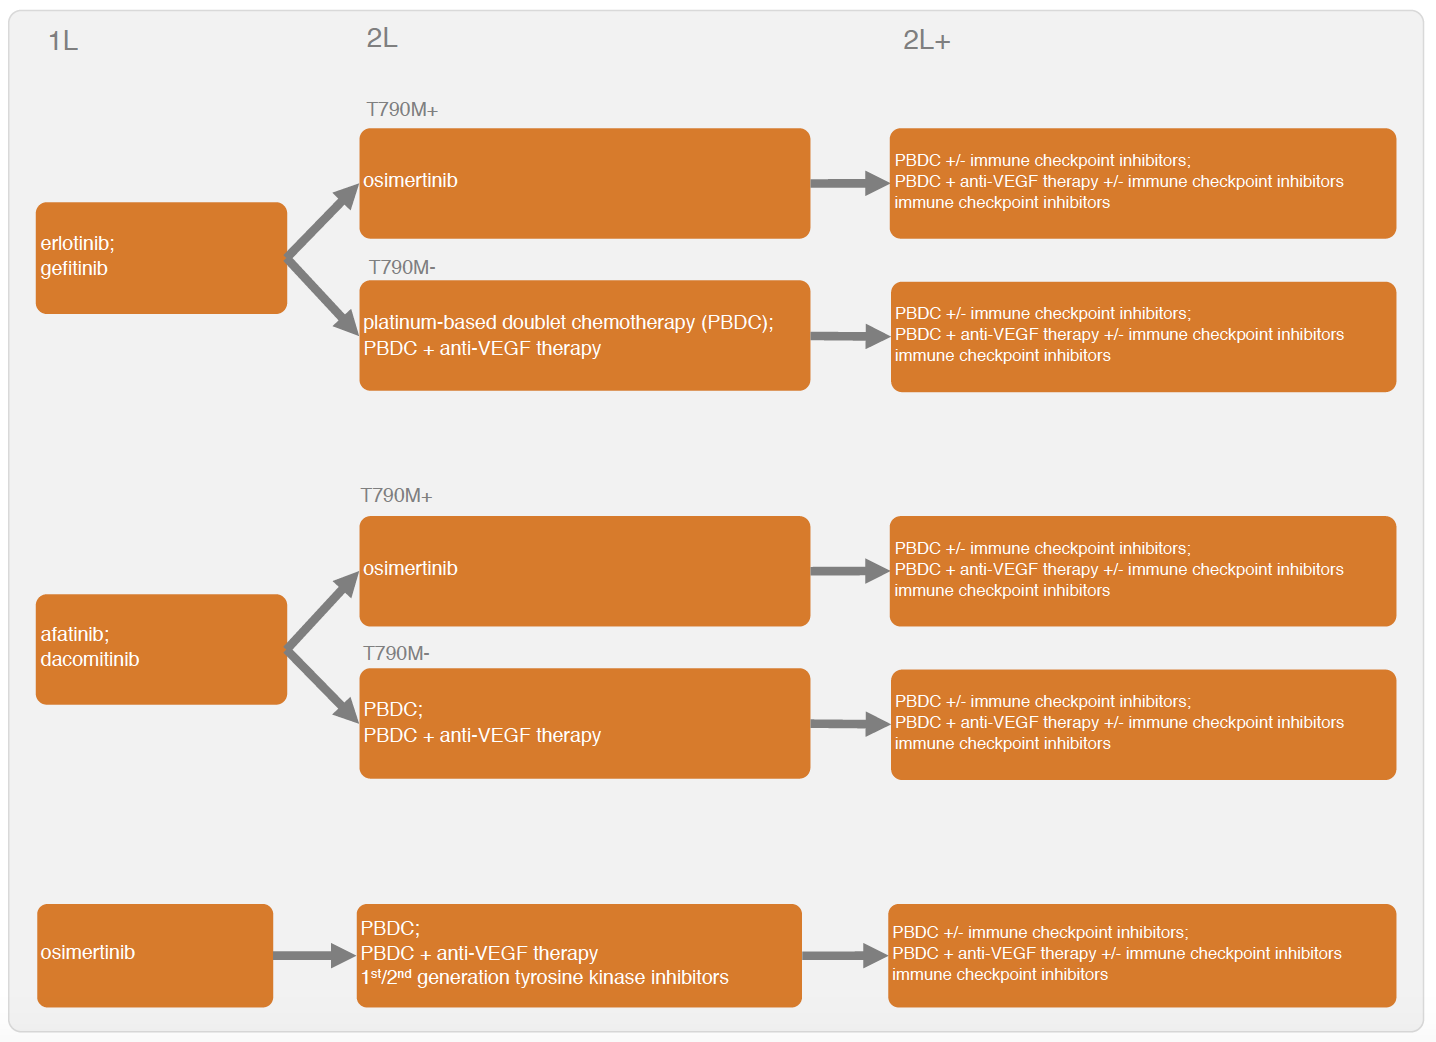
\includegraphics[max size={\textwidth}{\textheight}]{figs/treatment-strategies.png} 
\caption{Sequential treatment strategies of interest to be compared with the model}\label{fig:treatment-strategies}
\end{figure}

The IVI-NSCLC(egfr+) model is suitable for informing decisions for specific (sub)populations, but is not suitable for making predictions at the individual level, nor should it replace the patient-physician shared decision-making process.  Local decision makers can modify the model to perform analysis of value that reflect the local setting while accounting for all scientific uncertainty and help them understand the confidence with which they make decisions. 
 
The IVI-NSCLC(egfr+) model is not a value assessment framework, but a model that simulates the costs, health outcomes, and risks associated with sequential treatment sequences for metastatic EGFR+ NSCLC. It can therefore be used with any value framework preferred by the user. Currently, two methodologies for decision analysis are supported by the model: CEA based on cost per quality adjusted life year (QALY) expressed as net-monetary benefit (NMB) and MCDA \citep{keeney1993decisions}. 

The MCDA was implemented according to \citet{thokala2016multiple} and based on the following criteria: progression free survival (PFS), overall survival (OS), adverse events, expected time on first, second, and third line treatment, utility/quality of life, health care sector costs, productivity losses, route of administration (oral/injection/infusion) and time the medication has been on the market. The assessment of value can be performed from a health care sector perspective by only incorporating health care sector costs, or from a (limited) societal perspective by including productivity losses in addition.

\citet{garrison2017toward} suggest five concepts of value that researchers should consider adding to the standard cost per QALY based CEA: (i) a reduction in uncertainty from a diagnostic test; (ii) insurance value for healthy individuals due to reduction against physical risk; (iii) the value of hope for individuals who become risk-loving and would rather pay for a therapy with a long right survival tail than a therapy with a shorter right survival tail but an equivalent (or shorter) expected life-expectancy; (iv) real option value when a therapy allows an individual to benefit from future medical innovations; and (v) scientific spillovers when the benefits of an innovation cannot be entirely appropriated by the innovator.

The value of hope is most relevant for innovations that increase longevity and might be particularly well suited to the analyses of treatments for NSCLC. Traditionally, CEA focuses on maximizing expected QALYs; however, patients might be willing to take gambles (i.e., they become "risk lovers") and care about the variation in benefits and costs, not simply the means. If patients value hope, they may prefer the treatment with greater variability in survival over the treatment with less variability despite having the same expected survival. In contrast, if patients are risk-averse, they may prefer the latter to avoid an unlucky outcome. Either way, they have a preference for one intervention over its alternative that appear identical based on its average costs and benefits. Patients may place substantial value on a modest chance of a durable survival response, over and above average survival, and decision-makers acting on their behalf may want to consider this aspect when making population level decisions regarding the value of interventions. 

The IVI-NSCLC(egfr+) model allows users to incorporate value of hope into their analyses, while noting that the approach is less well-established than conventional cost-effectiveness analysis. Future versions of the IVI-NSCLC(egfr+) may consider incorporating other value components, such as insurance value.

\subsection{Evaluation of scientific uncertainty}
Decision models can be used to inform efficient use of health care resources, but often lead to scientific disagreements and mistrust among stakeholders. Model inputs are typically informed by a formal evidence synthesis to ensure all relevant evidence is considered. However, decisions regarding the mathematical structure relating model inputs to outputs are frequently made arbitrarily based on the idiosyncratic expertise of the model developer without evaluating the impact on findings. While robustness can be assessed by means of sensitivity analyses, these are typically limited to studying the impacts of varying model inputs. For any given disease, a variety of modeling approaches have typically been proposed in the literature. In order to evaluate the impact of these different approaches on estimates of value in a systematic way, we need flexible open-source models to not only capture the uncertainty in model input parameters (i.e. parameter uncertainty), but also capture alternative model structures (i.e. structural uncertainty). This flexibility facilitates demonstrating the implications of different areas of uncertainty and leads to a better understanding of the reasons why value estimates can vary.


\section{Iterative process}\label{sec:process}
In order for a decision model to remain relevant over time it needs to evolve along with the clinical evidence and scientific insights. An open-source approach facilitates iterative development and collaboration between multiple clinical and methodological experts. We will use a four-step process for the development of flexible decision or simulation models for value assessment:

1.	Public release of the model. The initial release of an OSVP model must be flexible and allow users to choose from a large number of plausible model structures and approaches based on clinical practice and previous modeling efforts.

2.	Invite feedback and suggested improvements to the model in a public comment period.

3.	A panel of experts determines which of the evidence-based suggestions for improvement suggested in Step 2 should be implemented by means of a modified Delphi process.

4.	Revise the model based on the feedback from the technical expert panel in Step 3.
The four-step process is designed to be repeated many times so that the modeling approach and evidence considered can be refined over time. 


\section{Components}\label{sec:components}
Version 1 of the IVI-NSCLC(egfr+) model is designed to provide a starting point for open debate. To facilitate transparency, understanding, debate and collaboration among diverse stakeholders, the IVI-lung model will consist of the following components available in the public domain:

\textbf{Source code:} R and C++ code for the model are available in an IVI GitHub repository. Modelers and programmers may adapt the source code for their own purposes or collaborate to improve the code.

\textbf{R package:} The model will be released as an R-package with documentation available online. Researchers can use the package to run the model for custom analyses. Use of the package is recommended when performing analyses for scientific research.

\textbf{Detailed model documentation:} This document provides extensive technical details on the model structure, statistical methods for parameter estimation, and source data.

\textbf{Expert Model Interface:} For users not well-versed in the programming language, a web application for running the model online is provided. The web application is designed for custom analyses and allows users full control over the treatments, patient population, model structures, parameter values, and simulation settings.

\textbf{Value Tool:} An important aim of OSVP is to obtain feedback from as many relevant stakeholders as possible. A general audience web-application has been developed, allowing those who are not experts in modeling or health economics, to interact with the model.


\section{Model structure}\label{sec:model-structure}
\subsection{Disease model}
The IVI-NSCLC is an individual-level continuous-time state transition model (CTSTM) in which patients can either have stable disease, progressed disease, or have died. Sequential treatment can be incorporated into the CTSTM by expanding the number of health states according to the number of treatment lines. In general, one can define a health state for each treatment line, a health state after progression on the final line, and a death state, so a model with n treatment lines will have n+2 health states. A patient with stable disease moves to the second treatment in a sequence after progression on the first treatment, to the third treatment after progression on the second treatment, and so on. A patient can die at any time. Unfortunately, the evidence base is currently too limited to explicitly model the transition rates by line of treatment according to \autoref{fig:treatment-strategies} and a simplified model structure is needed. Two options are available with the IVI-NSCLC model: The sequence of 1L, 2L, and 2L+ treatment can be represented with a four-state according to \autoref{fig:model-structure-4-states} or a three-state model according to \autoref{fig:model-structure-3-states}. 

The hazard rate, $\ h^{qr} $ \textit{(u)} for a transition from state \textit{q} to state \textit{r} at time \textit{u} follows different parametric distributions including the exponential, Weibull, Gompertz, log-logistic, and fractional polynomial distributions as estimated with a multi-state network meta-analysis (NMA). In the individual-level model, time to each state \textit{r} that can be entered from state \textit{q} is sampled based on time-varying hazard rates and patients' transition to the state with the shortest sampled time.

The parameterization of transitions between health states allows incorporating potentially relevant prognostic factors or effect-modifiers. This would also facilitate including carry-over effects from one line of treatment to the next, once such data becomes available.


\begin{figure}
\centering
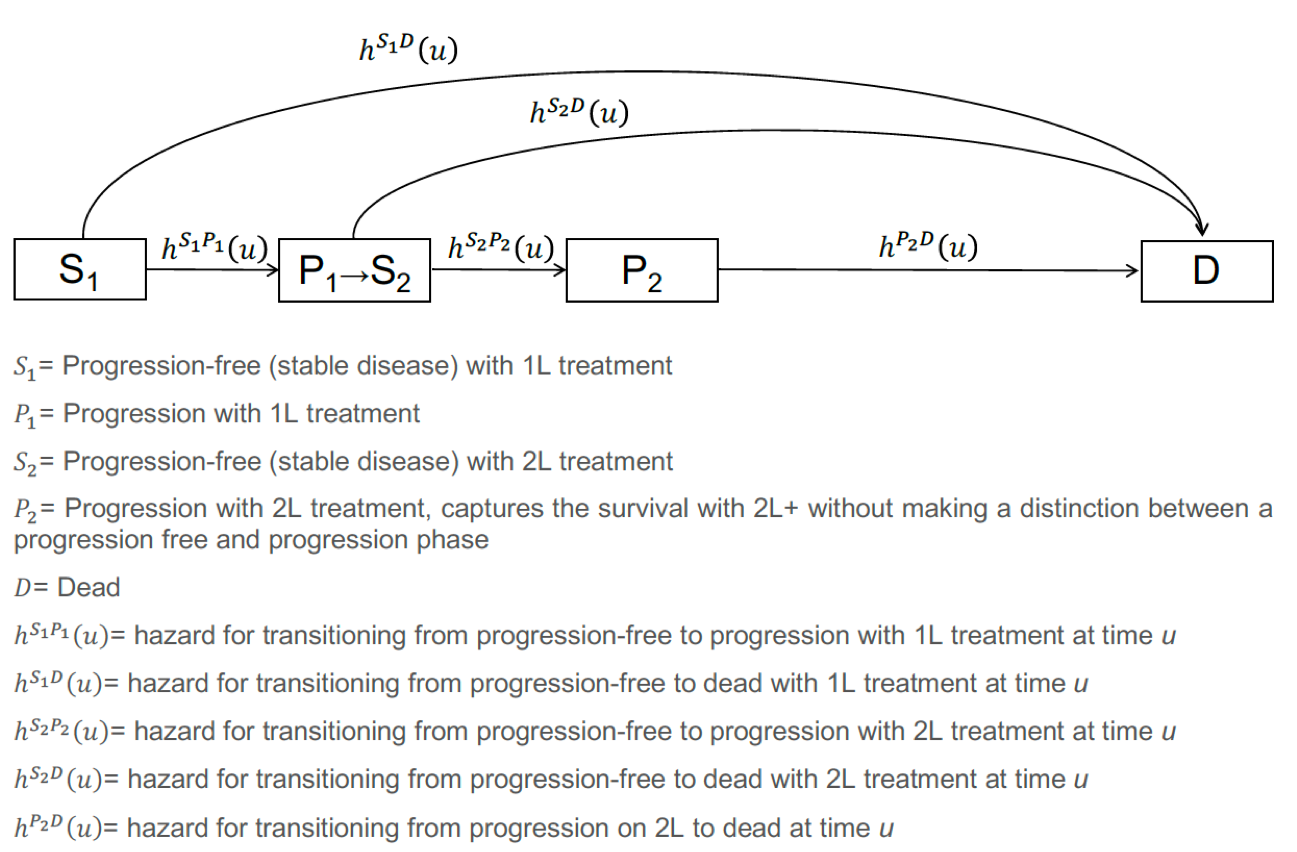
\includegraphics[max size={\textwidth}{\textheight}]{figs/model-structure-4-states.png}
\caption{Model structure with 4 states describing development of disease over time for a sequence starting with 1L, followed by 2L and 2L+ treatment; 2L+ treatment is captured with the L2 progression state}\label{fig:model-structure-4-states}
\end{figure}

\begin{figure}
\centering
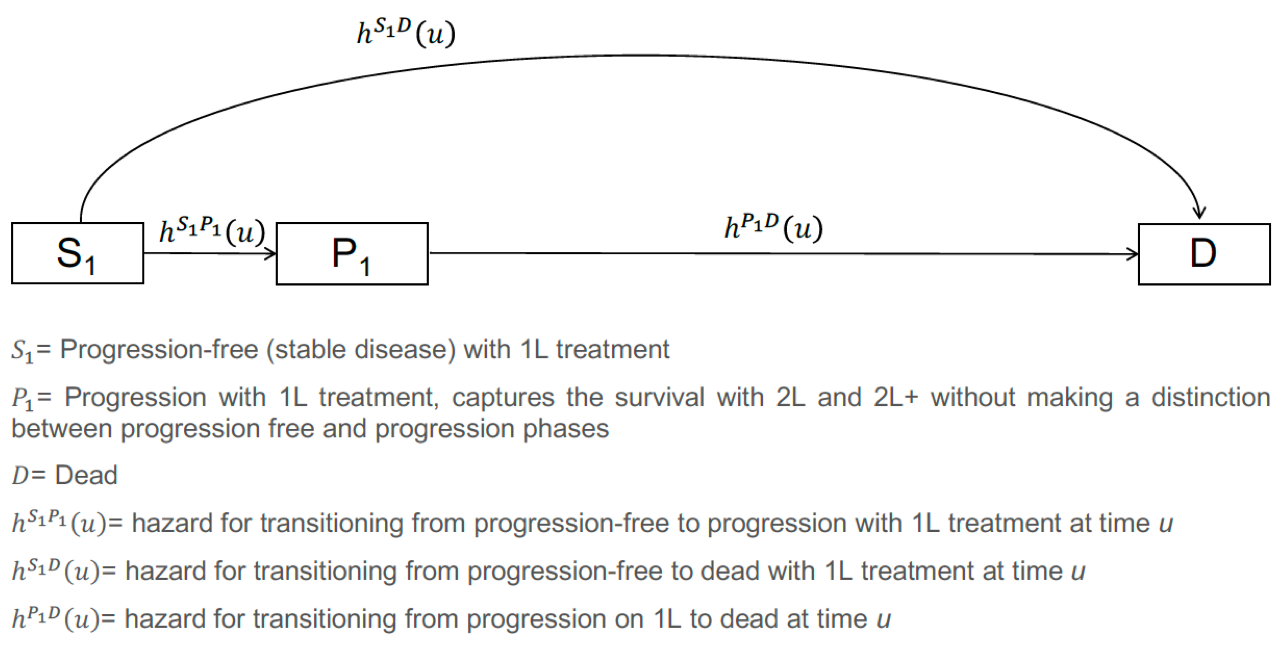
\includegraphics[max size={\textwidth}{\textheight}]{figs/model-structure-3-states.png}
\caption{Alternative model structure with 3 states describing development of disease over time for a treatment sequence starting with 1L until death; 2L and 2L+ treatment is captured with the progression state}\label{fig:model-structure-3-states} 
\end{figure}


\FloatBarrier

\subsection{Adverse events}
The model includes multiple distinct adverse events associated with 1L treatment. For each treatment and each patient, the model samples whether each adverse event occurs from a binomial distribution.

\subsection{Cost and utility}
All non-death health states are associated with utility and cost values. Cost values are separated into distinct categories (e.g., drug acquisition and administration costs, costs due to inpatient hospitalizations, etc.). Because we did not find strong evidence to the contrary, we assumed that utility and cost values remain constant over time within a given health state, but the model is also flexible enough to estimate utility and cost values that vary over time in a general manner. Adverse events cause utility decrements and more serious adverse events--such as those that require hospitalizations--increase health care costs. 

Drug acquisition and administration related costs are modeled based on standard clinical practice. For example, consider a case in which a therapy is dosed daily. Then costs will accrue each day until disease progression and the patient switches to the next treatment in the sequence. Another possible scenario is that dosing is based on fixed cycles. In these cases, costs will accrue until the end of a cycle or until the patient switches treatment due to disease progression. Other scenarios will be considered as required. 

The value of hope is illustrated with the model assuming representative relationships between utility values for each of the health states as a function of time reflecting risk-seeking and risk-averse behavior. 

Adverse events cause utility decrements and more serious adverse events--such as those that require hospitalizations--increase health care costs. 

\subsection{Patient heterogeneity}
The model is sufficiently flexible so that all model parameters (i.e., the parameters of probability distributions characterizing health state transitions, adverse event rates, costs, and utility) can depend on patient characteristics. In other words, we modeled input parameters as a function of covariates so that they can vary across individuals and treatments. That is, a given parameter, $\ a_{jt} $, for individual \textit{j} using treatment \textit{t} is modeled as $ \alpha_{jt} $ = $ \textit{g}^{-1} (X_{jt}\beta) $ where $ \textit{g}^{-1} $ (.) is an inverse transformation function. However, the extent heterogeneity can be modeled depends on the level of detail in the available evidence. We modeled heterogeneity based off of the level of evidence available. 

\subsection{Rationale for individual-level simulation}
Our primary motivation for using an individual-level model relates to the distinction between "clock forward" and "clock reset" approaches to parameter estimation. In the "clock reset" approach, time \textit{u} in $\ h^{qr} $ \textit{(u)} resets to 0 after each transition whereas in the "clock forward" approach, time \textit{u} refers to time since the start of the model. If a "clock forward" approach is used, then health state probabilities can be calculated analytically using the \citet{aalen1978empirical} estimator and a cohort CTSTM can be used; conversely, if a "clock reset" approach is taken, then individual-level simulation-based approaches must be used to estimate health state probabilities \citep{putter2007tutorial}, \citep{de2011mstate}, \citep{jackson2016flexsurv}. In our case, each line specific multi-state NMA is a "clock-forward" model; however, when modeling sequential treatment multiple multi-state NMAs are used so the disease model is a mixture between the two: a "clock forward" model is used for each treatment but time \textit{u} resets each time a patient begins a new treatment. To accommodate a mixture of "clock reset" and "clock forward" approaches, we use an individual-level model. 


\section{Model outcomes}\label{sec:model-outcomes}
The model simulates the health outcomes, risks, and costs associated with alternative treatment strategies in oncology. The model's time horizon can be selected by the user and will default to a lifetime horizon. The health outcomes, risks, and costs will be combined to assess value using two frameworks: CEA and MCDA. Both disaggregated model outcomes and value estimates will be based on mean values (i.e., averages across all simulated patients). An overview of all model outcomes is shown in \autoref{tbl:model-outcomes}. Additional details are provided in the text below.  

\begin{table}[!ht]
\begin{center}
\begin{threeparttable}
\caption{Model outcomes} \label{tbl:model-outcomes}
\begin{tabular}{p{0.3\linewidth}p{0.7\linewidth}}
\hline
\multicolumn{1}{l}{Category} & \multicolumn{1}{l}{Outcomes}\\
\hline
Health outcomes & Health state probabilities; progression free survival \& overall survival; quality-adjusted life-years\\
&\\
Risks & Adverse events (diarrhea, dry skin, elevated alanine transaminase, elevated aspartate transaminase, eye problems, paronychia, pneumonitis, pruritus, rash, stomatitis)\\
&\\
Health care sector costs & Drug acquisition and administration costs; adverse event costs; costs from inpatient hospital stays; costs from hospital outpatient or doctor office visits\\
&\\
Non-health care sector costs & Productivity losses \\
&\\
Value assessment & Cost-effectiveness analysis; multi-criteria decision analysis\\
\hline
\end{tabular}
\scriptsize
\end{threeparttable}
\end{center}
\end{table}

\subsection{Health outcomes}
The primary health outcome is the probability that a patient is in a given health state at a given point in time following treatment initiation. A survival curve was generated from the health state probabilities as one minus the probability that a patient has died. Since the model is an individual patient simulation, life expectancy is just the average time of death across simulated patients. Life-years was calculated as age at death minus age at treatment initiation. QALYs are weighted life-years, with weights equal to the utility values assigned to states.  Discounted QALYs were also calculated using a default discount rate of 3 percent.

\subsection{Risks}
The model calculates the expected number of adverse events per patient as the mean number of adverse events experienced by patients during the simulation. To improve interpretability, this number is reported as the expected number of adverse events per 1,000 patients. Both the expected number of total adverse events and the expected number of adverse events by type are reported.

\subsection{Costs} 
Costs are calculated for multiple categories and separated into health care sector and non-heath care sector costs as recommended by the \citet{sanders2016recommendations}. Health care sector cost categories included drug acquisition and administration costs, adverse events costs, the costs of inpatient hospital stays, and costs from hospital outpatient and doctor office visits. Non-health care sector costs include productivity losses. We used both human-capital approach and friction-cost approach to estimate productivity losses associated with the different treatment sequences. The level of detail regarding productivity related cost estimates that were incorporated is based on the available data in the literature.

\subsection{Value assessment} 
Value can be assessed using two frameworks: CEA and MCDA. If CEA is used for value assessment, then the value of treatment is estimated using the NMB. CEA from a societal perspective includes productivity losses while analyses from a health care sector perspective do not.

With MCDA, the value of each treatment strategy is based on a "total value" score. The score is calculated in three steps. First, a number of distinct criteria are assigned values on a common scale, for instance, ranging from 0 to 100. Second, each criterion is assigned points, say, ranging from 0 to 10, which is, in turn, used to calculate a weight by dividing each criterion's points by the sum of points across all criteria. For example, if there were 3 criteria and each criterion was given a score of 5, then each criterion would receive a weight of 1/3. If, on the other hand, the three criteria were given scores of 2.5, 5, and 7.5, then they would be given weights of 0.167, 0.33, and 0.5, respectively. Third, to aggregate results, we multiplied the value of each criterion on the common scale by its weight and sum the weighted scores across criteria. Future iterations of the model will consider using the Patient Experience Study to inform the baseline weights across attributes. 


\section{Source data and parameter estimation}\label{sec:data}
Key parameters for the model relate to: (i) treatment effects in terms of transitions between the health states; (ii) adverse events; (iii) utilities; (iv) healthcare resource use; and (v) productivity. Parameter estimates for the current version of the IVI-NSCLC(egfr+) model are based on currently available published evidence identified by means of a systematic literature review and synthesized with meta-analysis techniques where appropriate. 

\subsection{Treatment effects for transition rates} \label{subsec:data-transprobs}
Relevant evidence to estimate treatment effects with the alternative TKIs and chemotherapy regimens in terms of transitions between the health states was obtained with a systematic literature review of randomized controlled trials (RCTs) evaluating the efficacy of relevant competing interventions for the treatment of adult patients with metastatic EGFR+ non-squamous NSCLC by line of treatment (i.e. 1L, 2L, and 2L+) in terms of OS and PFS. Details regarding eligibility criteria, search strategies, included studies, extracted information regarding study and patient characteristics, results, and KM curves are provided in \hl{(Appendix X)}. 
The identified evidence base was used to 1) estimate the relative treatment effects for each 1L treatment versus a defined reference treatment; 2) estimate the absolute effects with the corresponding 1L reference treatment; and 3) estimate the absolute treatment effects with 2L treatment options. 

\subsubsection{Relative treatment effects with 1L therapy}
Relative treatment effects of the competing TKIs in comparison to gefitinib for the 1L treatment of EGFR+ NSCLC were estimated by means of a Bayesian network meta-analysis (NMA) using alternative fixed and random effects models. 

RCTs are considered the gold standard to assess treatment effects of medical interventions. For many disease states there are multiple competing interventions to choose from. However, an RCT will rarely include all competing interventions of interest for a particular disease state when there are more than two relevant treatment options available. As such, an individual trial rarely provides all the information needed to guide evidence-based treatment selection. When each RCT compares only a subset of the interventions of interest---it may be possible to represent the evidence base as a network where all trials have at least one intervention in common with another trial. Such a network of trials involving treatments compared directly, indirectly, or both, can be synthesized by means of a network meta-analysis \hl{(add reference)}. As a result we not only get pooled results of available treatment comparisons studied in a head-to-head fashion but also relative treatment effects between interventions not compared directly. In order to ensure that a network meta-analysis are not affected by bias due to differences in prognostic factors between studies, we want to only consider the relative treatment effects of each trial. This implies that all interventions have to be part of one network of trials where each trial has at least one intervention in common with another trial.  

Patients are randomized only within trials, not across trials, so there is a risk that patients participating in different trials differ with respect to demographic, disease or other characteristics. In addition, features of the trials themselves may differ. If these trial or patient characteristics are effect modifiers, i.e. they affect the treatment effects of an intervention versus a control, then there are systematic differences in treatment effects across trials. Systematic differences in known and unknown effect-modifiers among studies comparing the same interventions in direct fashion result in between-study heterogeneity. An imbalance in the distribution of effect modifiers between studies comparing different interventions will result in transitivity or consistency violations and therefore biased indirect comparisons.

The RCTs that were part of one evidence network and were deemed sufficiently similar were included in the NMA. The evidence network for 1L treatments is presented in \autoref{fig:RCT network-1L}. Information regarding the distribution of patients characteristics across the studies in the network  are presented in \hl{(Appendix X)}. 

\begin{figure}
\centering
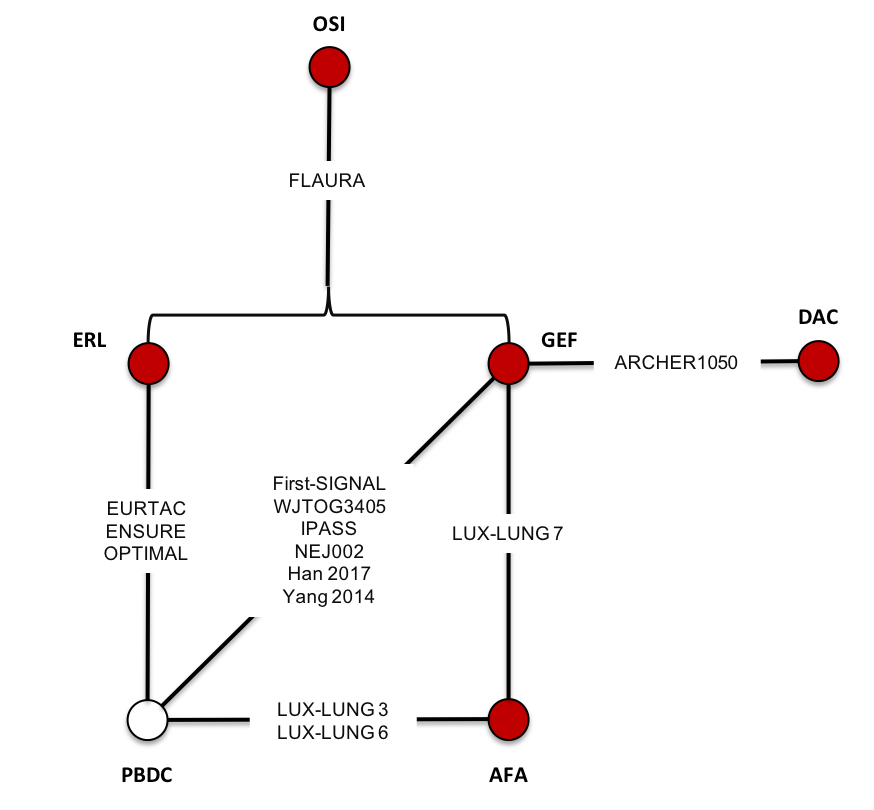
\includegraphics[max size={\textwidth}{\textheight}]{figs/RCT-network-1L.png}
\caption{Network of RCTs to estimate relative treatment effects regarding PFS and OS with 1L therapies}\label{fig:RCT network-1L}
\end{figure}

\FloatBarrier

\subsubsubsection{Network meta-analysis model}
Traditionally, NMAs in oncology are based on separate analyses for OS and PFS, with relative treatment effects estimated using reported hazard ratios (HR). There are two limitations of this approach. First, HR estimates rely on the proportional hazard assumption, which is implausible if the hazard functions of the competing interventions cross \citep{dias2018network}. Second, separate analyses of OS and PFS ignore the structural relationship between stable disease, progression, and death and implicitly assume that transition probabilities for stable to death and progression to death are equal.

We overcome these limitations by introducing a multi-state NMA that explicitly estimates each possible transition in a 3-state model---stable to progression, stable to death, and progression to death--and modeling time-varying hazard rates and relative treatment effects with known parametric survival functions or fractional polynomials. Our approach is illustrated in \autoref{fig:multistate-nma} and expressed mathematically as follows:

\FloatBarrier


\begin{figure}
\centering

\includegraphics[max size={\textwidth}{\textheight}]{figs/multistate-nma.png}
\caption{Relationship between stable disease (S), progression (P) and death (D) as used in the multi-state network meta-analysis model}\label{fig:multistate-nma}
\end{figure}



\begin{equation}\label{eqn:multistate-nma}
\begin{aligned} 
% SP transition
\ln\left(h_{ik}^{SP}(u)\right) &= 
\begin{cases}
\alpha_{1ik} + \alpha_{2ik}u^{p_1} + \alpha_{3ik}u^{p_2} & \text{if } p_1 \neq p_2 \\ 
\alpha_{1ik} + \alpha_{2ik}u^{p} + \alpha_{3ik}u^{p}\ln(u) & \text{if } p_1 = p_2 = p \\ 
\end{cases}\\ 
% SD transition 
\ln\left(h_{ik}^{SD}(u)\right) &=
\alpha_{4ik}\\
% PD transition
\ln\left(h_{ik}^{PD}(u)\right) &=
\alpha_{5ik} + \alpha_{6ik}u^{p_1}\\ 
\\
% Coefficient matrix
\begin{pmatrix}
\alpha_{1ik} \\
\alpha_{2ik} \\
\alpha_{3ik} \\
\alpha_{4ik} \\
\alpha_{5ik} \\
\alpha_{6ik} \\
\end{pmatrix}
&= 
\begin{pmatrix}
\mu_{1ik} \\
\mu_{2ik} \\
\mu_{3ik} \\
\mu_{4ik} \\
\mu_{5ik} \\
\mu_{6ik} \\
\end{pmatrix} 
+
\begin{pmatrix}
\delta_{1,ik} \\
d_{2, t_{ik}} - d_{2, t_{i1}}  \\
0 \\
0  \\
d_{3, t_{ik}} - d_{3, t_{i1}} \\
0 \\
\end{pmatrix} \\\\ 
% Random effects
\delta_{1,ik} &\sim N(d_{1, t_{ik}} - d_{1, t_{i1}}, \sigma_{d_{1}}^{2}) 
\end{aligned}
\end{equation}

where $u^0= \ln(u)$ and ${d_{1,1}}=0$, ${d_{2,1}}=0$, and ${d_{3,1}}=0$
\\

$h_{ik}^{SD}(u)$, $h_{ik}^{PD}(u)$, and $h_{ik}^{SD}(u)$ are the the hazard rate for disease progression, dying post-progression, and dying pre-progression, respectively, in study $i$ for treatment arm $k$ at time $u$. The $\alpha_{\cdot ik}$ are regression coefficients that represent the scale and shape parameters of the log hazard function in study $i$ for treatment arm $k$. The $\mu_{\cdot i}$ reflect the study effects regarding the scale and shape parameters in each study $i$. The $\delta_{1,ik} $ are the study specific true underlying relative treatment effects regarding the scale of the log hazard function for the transition from stable to progression, which are described by a normal distribution with an average effect for treatment $t$ relative to reference treatment 1, ${d_{1,1t}}$, and between study heterogeneity $\sigma_{d_{1}}^{2} $.  ${d_{2,1t}}$ are the treatment specific relative effects regarding the first shape parameter of the log hazard function for the transition from stable to progression relative to the reference treatment 1 (i.e. gefitinib). To facilitate parameter estimation, we assumed that treatment has no effect on the 2nd shape parameter. Transition rates between stable disease and death are likely to be relatively small and therefore assumed to be independent of time and the same for all treatments. ${d_{3,1t}}$ are the treatment specific relative effects regarding the scale parameter of the log-hazard function for the transition from progression to death relative to reference treatment 1 (i.e. gefitinib). 

When $p_{1}=0$ and $\alpha_{3ik}=0$ the log-hazard functions for the transitions between stable disease and progression, and progression and death follow a Weibull distribution. When $p_{1}=1$ and $\alpha_{3ik}=0$ these log-hazard functions follow a Gompertz distribution. When $\{(p_1, p_2) = (0, 0), (0,1)\}$ and $\alpha_{3ik}\neq0$, the log-hazard functions follow a second order fractional polynomial that are extensions of the Weibull and Gompertz model to allow for arc- and bathtub shaped log-hazard functions. 

A fixed effects model is obtained by replacing $\delta_{1,ik} \sim N(d_{1, t_{ik}} - d_{1, t_{i1}}, \sigma^2)$ with $\delta_{1,ik} = d_{1, t_{ik}} - d_{1, t_{i1}}$. 

If it is assumed that treatment has only a direct effect on the transitions from stable to progression, which can be reasonably defended when a particular treatment upon disease progression is discontinued, the model can be simplified by setting $d_{3, t_{i1}}=0$.


\subsubsubsection{Likelihood}
The model parameters were estimated based on the number of patients $r$ in each of the three health states (stable, progression and death) at time $u$ for each arm $k$ of each trial $i$ obtained from the published Kaplan-Meier (KM) curves for time points for which both PFS and OS were reported. Accordingly, a multinomial likelihood was used for the proportion of patients in each of the three health states at any time point for each arm of each trial ($S_{ik}(u)$, $P_{ik}(u)$, and $D_{ik}(u)$) according to: 

\begin{equation} \label{eqn:multinomial_likelihood}
\begin{aligned}
% Likelihood
(r_{ik}^{S}(u),r_{ik}^{P}(u),r_{ik}^{D}(u)) \sim multinomial(S_{ik}(u),P_{ik}(u),D_{ik}(u),n_{ik}(u))
\end{aligned}
\end{equation}

where $n_{ik}(u)=r_{ik}^{S}(u)+r_{ik}^{P}(u)+r_{ik}^{D}(u)$ and $S_{ik}(u)+P_{ik}(u)+D_{ik}(u)=1$
\\

Arbitrary hazard rate functions can be approximated with a set of discontinuous constant hazard rates over successive time intervals. The total follow-up time can be partitioned into $M$ successive non-overlapping intervals indexed by $m= 1, ..., M$. We refer to interval $m$ as $U_{m}$ and write $u \in U_{m}$ to denote $u_{m}\leq u<  u_{m+1}$. The length of $U_{m}$ is $\Delta u_{m} =u_{m+1}-u_{m}$. 

For each interval $m$, the proportions  $S_{ik}(u)$, $P_{ik}(u)$, and $D_{ik}(u)$ are related to the time-varying hazards $\ h_{ik}^{SP} (u) $,$\ h_{ik}^{SD} (u) $, $\ h_{ik}^{PD} (u)$ according to the following set of differential equations \citep{jansen2013multivariate}: 

\begin{equation} \label{eqn:diff_equations}
\begin{aligned}
% Differential equations
S_{ik}(u) &= S_{ik}(u_{m}) e^{-(h_{ikm}^{SP}+h_{ikm}^{SD})(u-u_{m})} \\
P_{ik}(u) &= P_{ik}(u_{m}) e^{-h_{ikm}^{PD}(u-u_{m})}+\frac{S(u_{m})h_{ikm}^{SP}(e^{-(h_{ikm}^{SP}+h_{ikm}^{SD})(u-u_{m})}-e^{-h_{ikm}^{PD}(u-u_{m})})}{h_{ikm}^{PD}-h_{ik}^{SP}-h_{ikm}^{SD}} \\
D_{ik}(u) &= 1-S_{ik}(u) - P_{ik}(u) \\
\end{aligned}
\end{equation}
\\

In order to estimate $h_{ikm}^{SP}$, $h_{ikm}^{SD}$, and $h_{ikm}^{PD}$ for each interval $m$,  data at three time points were used: $u_{m}$, $u_{m+\frac{1}{2}}$, and $u_{m+1}$. The obtained estimates of the hazards for interval $m$ were assigned to the time point corresponding to the mid point of the interval when used in the NMA.
\\

For time points of a trial for which only OS data was reported (and no PFS), the number of patients that survived time interval $m$ ($r_{ikm}^{OS}$) out of the number of patients alive at the beginning of interval ($n_{ikm}^{OS}$) were used for the model parameter estimation. A binomial likelihood was used for the conditional survival probabilities ($p_{ikm}^{OS}$):


\begin{equation} \label{eqn:binomial_likelihood}
\begin{aligned}
% Likelihood
r_{ikm}^{OS} \sim binomial(p_{ikm}^{OS},n_{ikm}^{OS})
\end{aligned}
\end{equation}
\\
The conditional survival probabilities inform $h_{ik}^{SD}(u)$ and $h_{ik}^{PD}(u)$ according to:

\begin{equation} \label{eqn:diff_equations_OS}
\begin{aligned}
% Differential equations OS
p_{ikm}^{OS} &= e^{-(h_{ikm}^{SD}+h_{ikm}^{PD})(u-u_{m})} \\
\end{aligned}
\end{equation}
where the obtained estimates of the hazards for interval $m$ assigned to the time point corresponding to the mid point of the interval when used in the NMA.
\\

\subsubsubsection{Prior distributions}
The following prior distributions for the parameters of the model expressed with \autoref{eqn:multistate-nma} were used:

\begin{equation} \label{eqn:multistate-nma-priors}
\begin{aligned}
% Prior for mu's
\begin{pmatrix}
\mu_{1i}  \\
\mu_{2i}  \\
\mu_{3i}  \\
\mu_{4i}  \\
\mu_{5i}  \\
\mu_{6i}  \\
\end{pmatrix} 
&\sim 
MVN\left(
\begin{pmatrix}
0  \\
0  \\
0  \\
0  \\
0  \\
0 \\
\end{pmatrix}, 
T_\mu
\right) 
\qquad
T_\mu =
\begin{pmatrix}
100 & 0 & 0 & 0 & 0 & 0 \\
0 & 10 & 0 & 0 & 0 & 0 \\
0 & 0 & 10 & 0 & 0 & 0 \\
0 & 0 & 0 & 100 & 0 & 0 \\
0 & 0 & 0 & 0 & 10 & 0 \\
0 & 0 & 0 & 0 & 0 & 10 \\
\end{pmatrix}\\\\
%
% Prior for ds
\begin{pmatrix}
d_{1, 1t}  \\
d_{2, 1t}  \\
d_{3, 1t}  \\
\end{pmatrix} 
&\sim 
MVN\left(
\begin{pmatrix}
0  \\
0  \\
0 \\
\end{pmatrix}, 
T_d
\right) 
\qquad
T_d =
\begin{pmatrix}
2 & 0 & 0  \\
0 & 1 & 0   \\
0 & 0 & 2  \\
\end{pmatrix} \\
%
\\
% Prior for between-study heterogeneity
\sigma_{d_{1}} &= uniform(0.2)  \\
\end{aligned}
\end{equation}

The prior distribution for the probabilities at the beginning of each interval, $u_{m}$ was: 

\begin{equation} \label{eqn:multinomial-prior}
\begin{aligned}
% Prior for probabilities at beginning of interval
(S_{ik}(u_{m}),P_{ik}(u_{m}),D_{ik}(u_{m})) \sim Dirichlet(0,0,0) \\
\end{aligned}
\end{equation}


\subsubsubsection{Model selection}
The residual deviance and the deviance information criterion (DIC) were used to compare the goodness-of-fit of the competing NMA models, i.e. fixed and random effects Weibull, Gompertz, and fractional polynomial models (See \hl{(Appendix X)}).\citep{dias2018network}. The DIC provides a measure of model fit that penalizes model complexity. In general, a more complex model results in a better fit to the data, demonstrating a smaller residual deviance. The model with the better trade-off between fit and parsimony has a lower DIC. A difference in the DIC of about 10 points is considered meaningful. 


\subsubsubsection{Estimated time-varying hazard ratios}
To be added

\begin{figure}[h]
\centering
%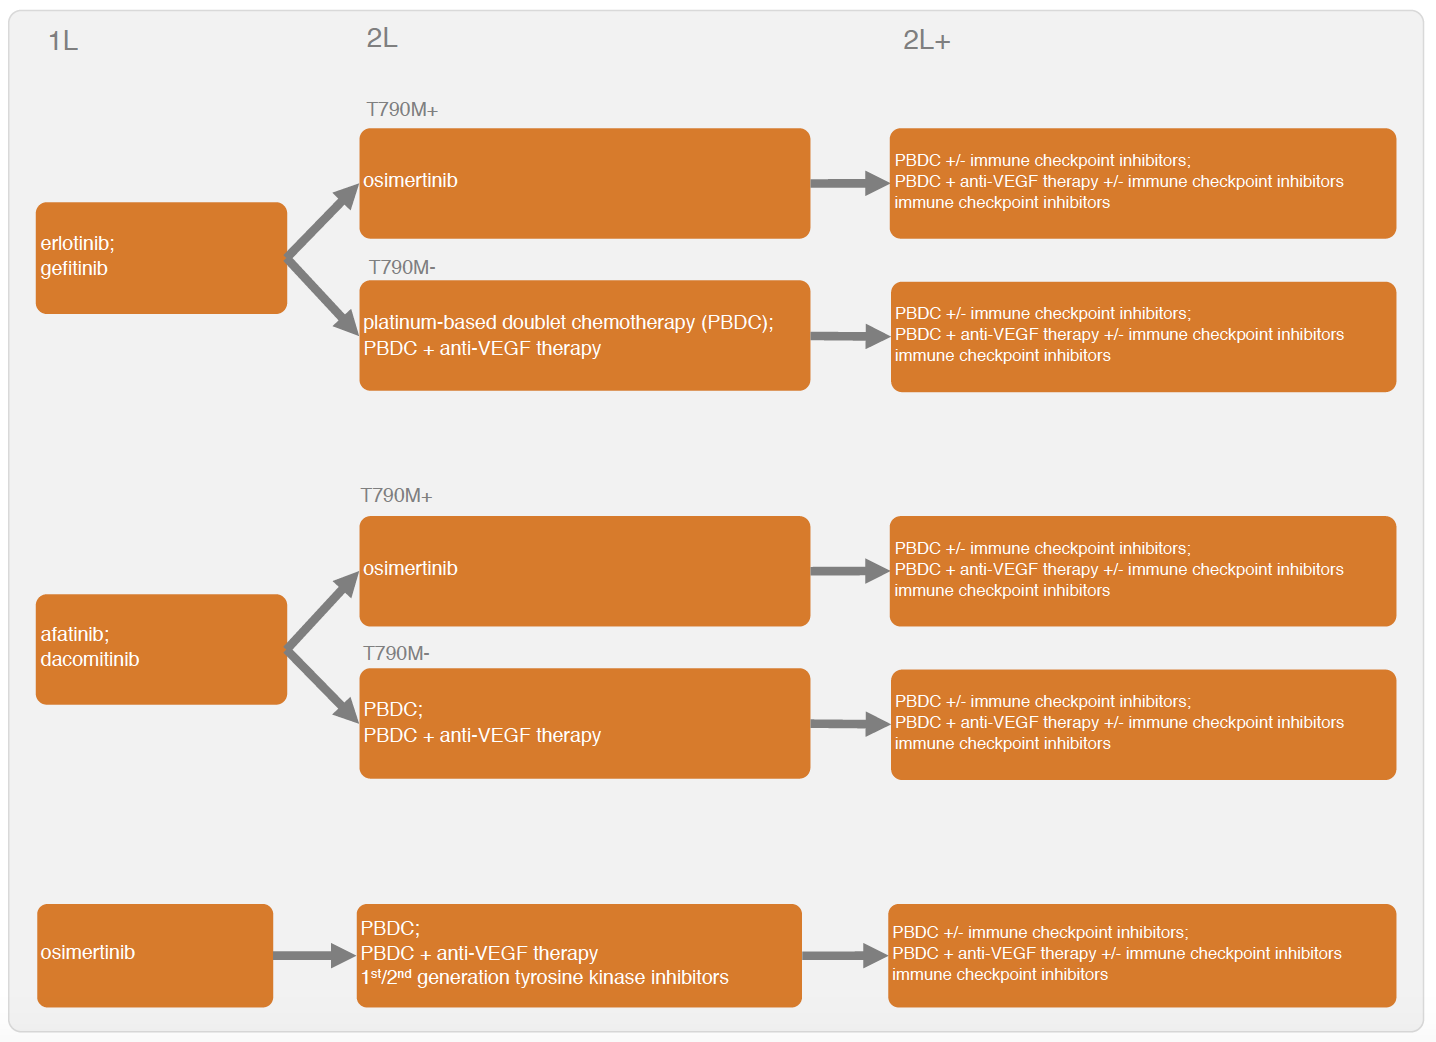
\includegraphics[max size={\textwidth}{\textheight}]{figs/treatment-strategies.png} 
\caption{First line estimates of hazard ratios from stable to progression relative to gefitinib from the multi-state network meta-analysis}\label{fig:hr-1L}
\end{figure}


\subsubsection{Absolute effects with 1L reference treatment}
Absolute effects with 1L therapy with the reference intervention, i.e. gefitinib, were estimated with the multi-state meta-analysis model expressed in \autoref{eqn:multistate-ma} with likelihoods and transformations according to \autoref{eqn:multinomial_likelihood}, \autoref{eqn:diff_equations}, \autoref{eqn:binomial_likelihood}, and \autoref{eqn:diff_equations_OS} based on the reported KM curves of all the gefitinib treatment arms of the available RCTs.

\begin{equation}\label{eqn:multistate-ma}
\begin{aligned} 
% SP transition
\ln\left(h_{i}^{SP}(u)\right) &= 
\begin{cases}
M_{1} + M_{2}u^{p_1} + M_{3}u^{p_2} & \text{if } p_1 \neq p_2 \\ 
M_{1} + M_{2}u^{p} + M_{3}u^{p}\ln(u) & \text{if } p_1 = p_2 = p \\ 
\end{cases}\\ 
% SD transition 
\ln\left(h_{i}^{SD}(u)\right) &=
M_{4}\\
% PD transition
\ln\left(h_{i}^{PD}(u)\right) &=
M_{5} + M_{6}u^{p_1}\\ 
\\
\end{aligned}
\end{equation}

where $u^0= \ln(u)$
\\

$h_{i}^{SD}(u)$, $h_{i}^{PD}(u)$, and $h_{i}^{SD}(u)$ are the underlying hazard rates for disease progression, dying post-progression, and dying pre-progression, respectively, in study $i$ at time $u$. The $M_{\cdot}$ represent the pooled scale and shape parameters describing the log hazard functions over time. As before, when $p_{1}=0$ and $M_{3}=0$ the log-hazard functions for the transitions between stable disease and progression, and progression and death follow a Weibull distribution. When $p_{1}=1$ and $M_{3}=0$ these log-hazard functions follow a Gompertz distribution. When $\{(p_1, p_2) = (0, 0), (0,1)\}$ and $M_{3}\neq0$, the log-hazard functions follow a second order fractional polynomial to allow for arc- and bathtub shaped log-hazard functions. 

\autoref{fig:hazards-gef-1L} shows the hazard functions for the transitions between stable, progression, and death with gefitinib for each fitted model.

The posterior distributions of $M_{\cdot}$ along with the parameters representing the relative treatment effects of each TKI relative to gefitinib ($d_{1, t}$), were used to simulate a posterior distribution for PFS and OS as displayed in \autoref{fig:surv-1L} for each 1L treatment and each fitted model. 


\begin{figure}[h]
\centering
%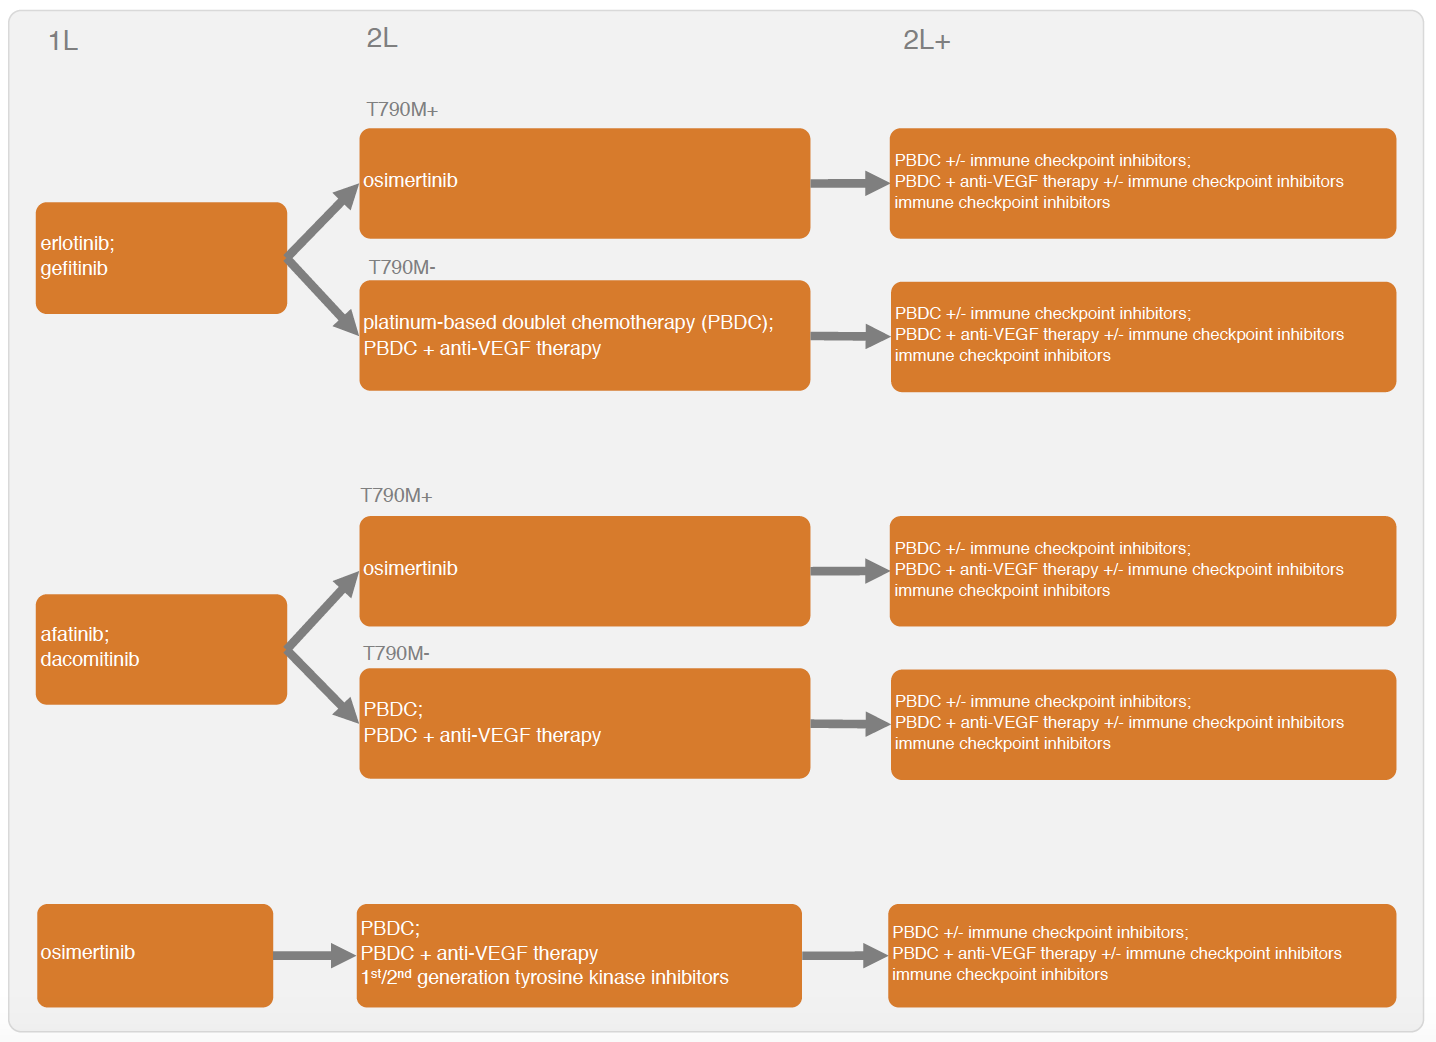
\includegraphics[max size={\textwidth}{\textheight}]{figs/treatment-strategies.png} 
\caption{First line estimates of hazard rates over time for transitions between S, P and D with gefitinib from the multi-state meta-analysis}\label{fig:hazards-gef-1L}
\end{figure}


\begin{figure}[h]
\centering
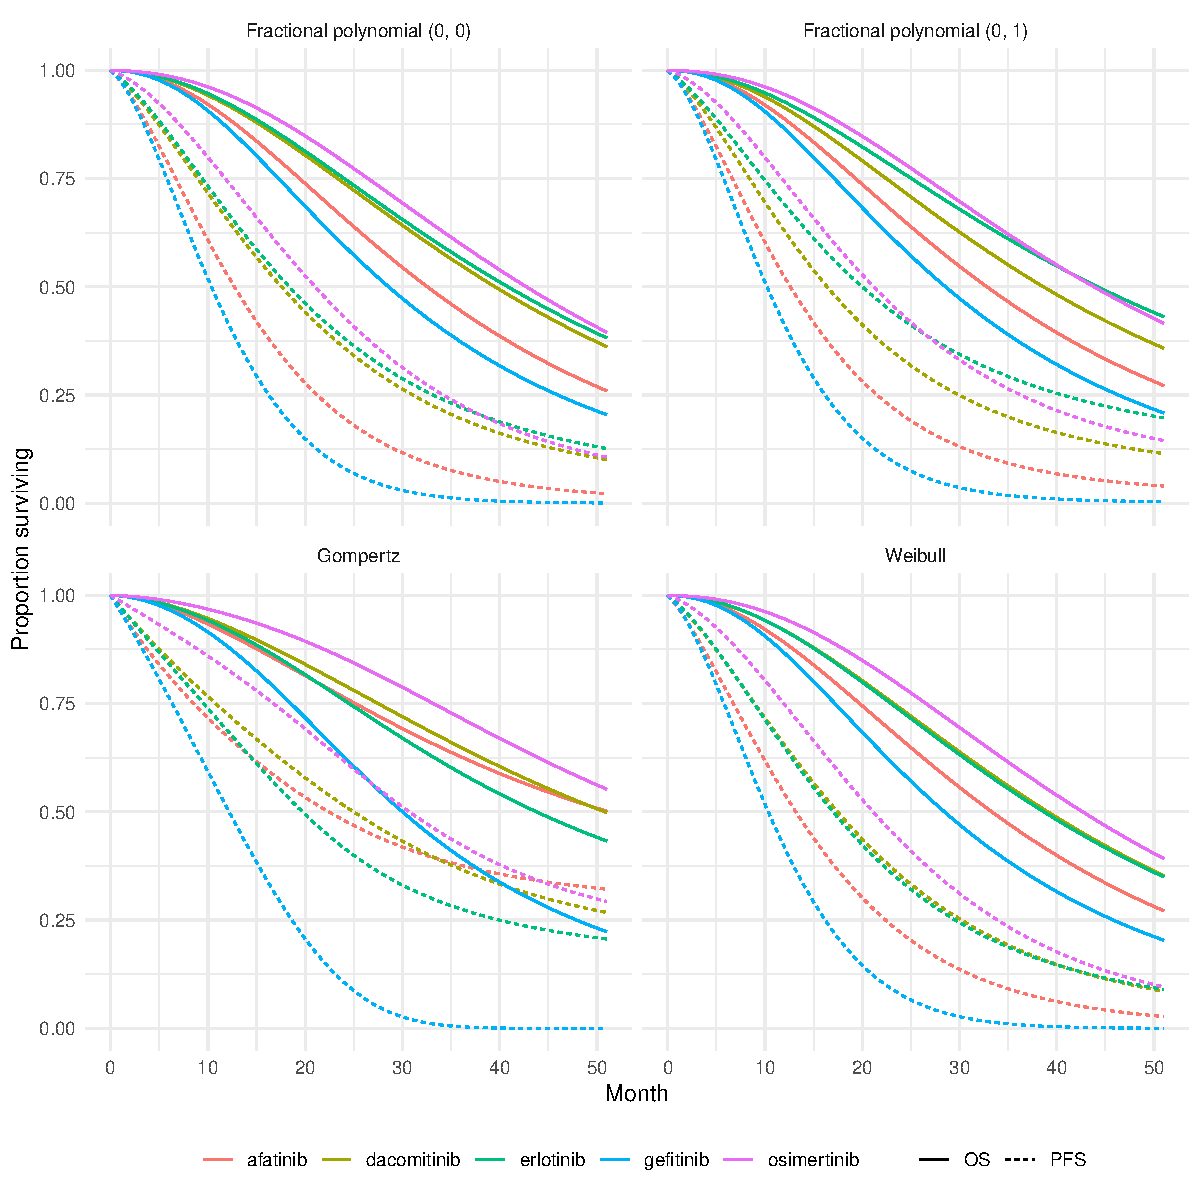
\includegraphics[max size={\textwidth}{\textheight}]{figs/surv-1L.pdf} 
\caption{First line estimates of progression-free survival and overall survival for the competing interventions obtained with the multi-state (network) meta-analysis}\label{fig:surv-1L}
\begin{minipage}{\linewidth}
\footnotesize
Notes: The simulated posterior distribution of the parameters of the Bayesian multi-state NMA was used to simulate a distribution of progression-free survival and overall survival curves. The curves in the figure are posterior means. Curves with credible intervals are shown in the appendix.
\end{minipage}
\end{figure}

\FloatBarrier


\subsubsection{Absolute effects with 2L therapy}
For the 2L treatment options, the available number of RCTs among patients who progressed on 1L TKI were limited. For T790M positive patients, the transition rates with osimertinib were estimated based on data from two RCTs according to \autoref{eqn:multistate-ma}.  Regarding other possible treatments, there was only data available for PBDC from three RCTs, which were used to estimate transition rates according to \autoref{eqn:multistate-ma} as well. In the absence of RCT evidence, these estimates were assumed to be representative of the other 2L treatment regimens presented in \autoref{fig:treatment-strategies} for both an all-comer population and a T790M mutation negative population. \autoref{fig:hazards-2L} shows the hazard functions for the transitions between stable, progression, and death for each fitted model and \autoref{fig:surv-2L} shows the corresponding PFS and OS curves.

\FloatBarrier



\begin{figure}[h]
\centering
%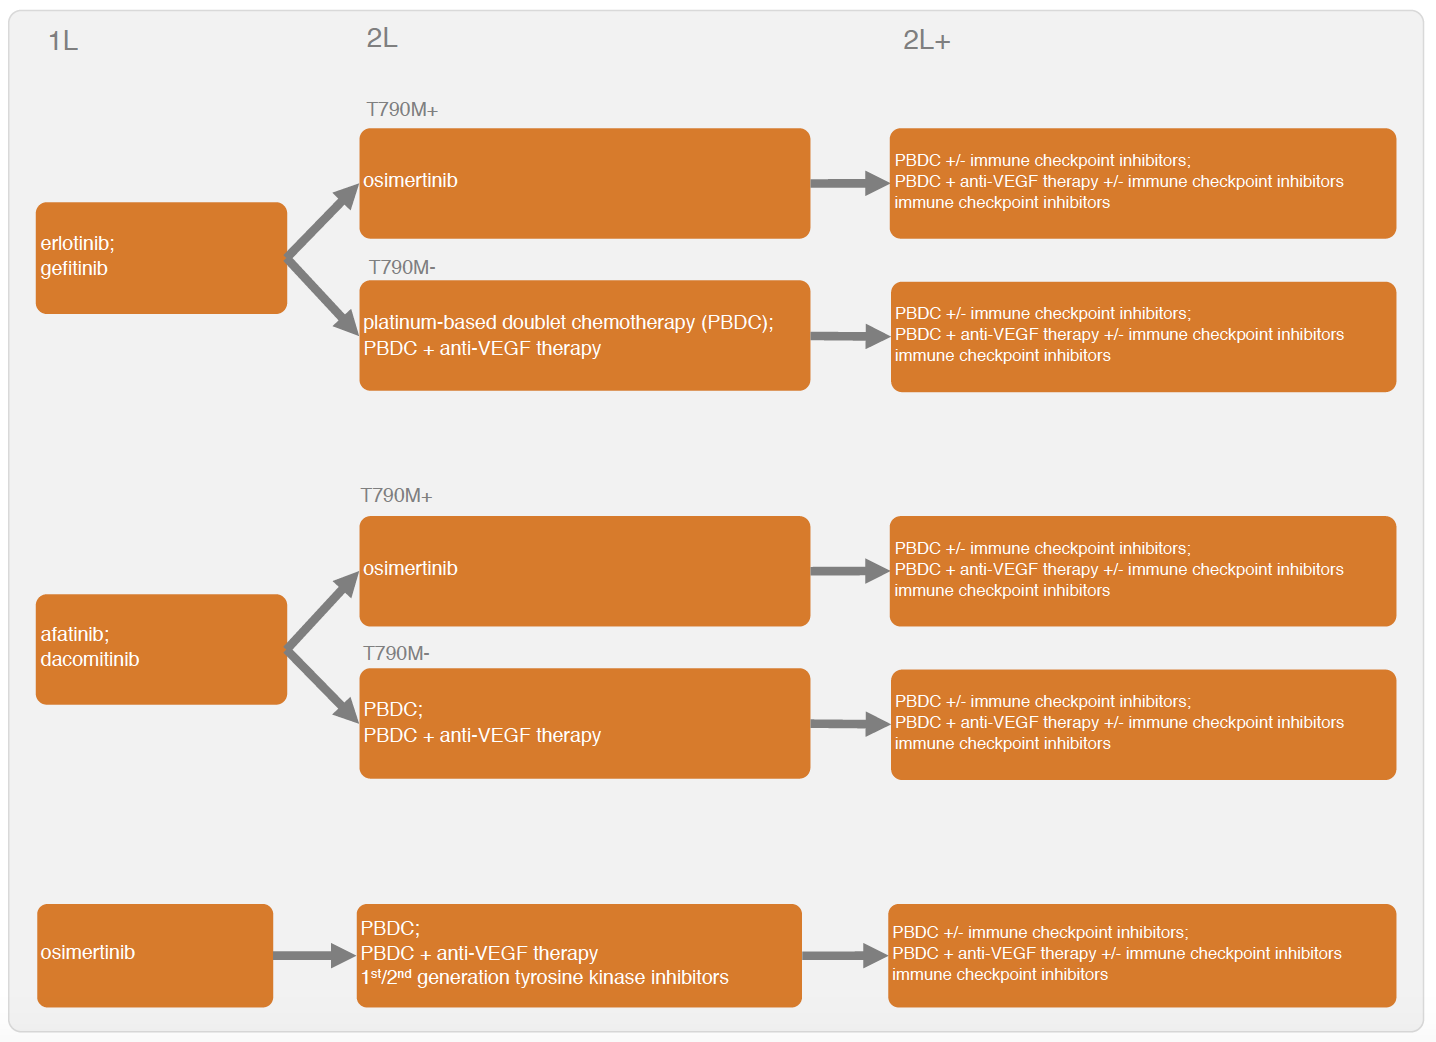
\includegraphics[max size={\textwidth}{\textheight}]{figs/treatment-strategies.png} 
\caption{Second line estimates of hazard rates over time for transitions between S, P and D from the multi-state meta-analysis}\label{fig:hazards-2L}
\end{figure}



\begin{figure}
\centering
\begin{subfigure}{\textwidth}
\centering
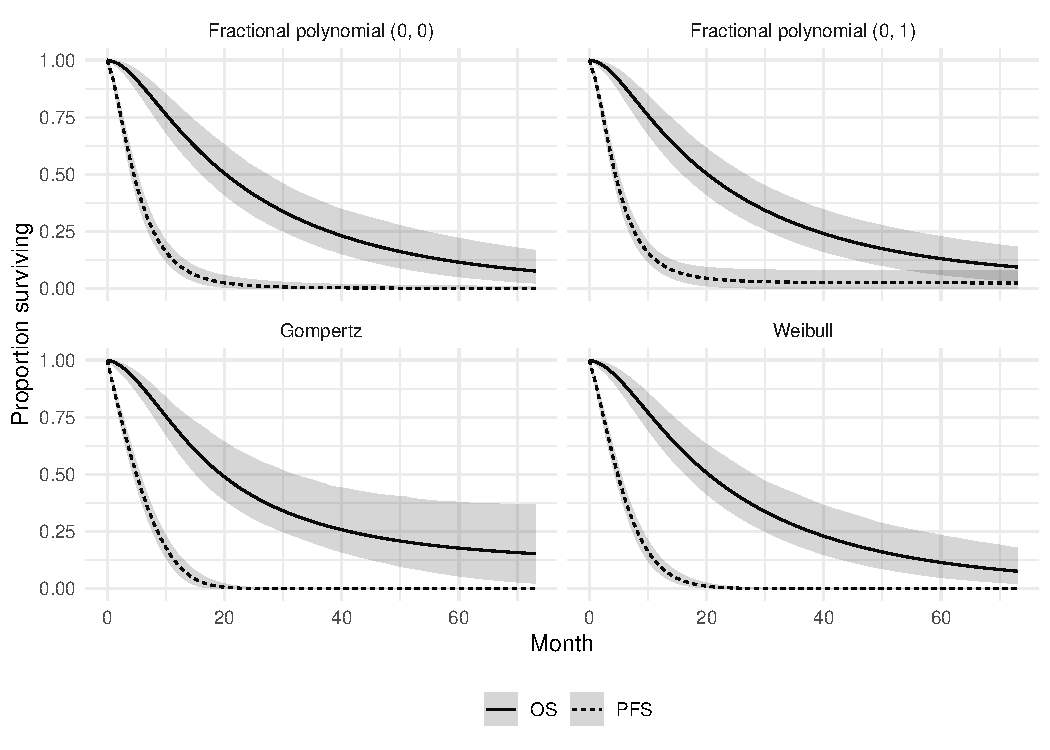
\includegraphics[max size={.8\textwidth}{.8\textheight}]{figs/surv-2L-pbdc.pdf}
\caption{Platinum based doublet chemotherapy} \label{subfig:surv-2L-pbdc}
\end{subfigure}
\begin{subfigure}{\textwidth}
\centering
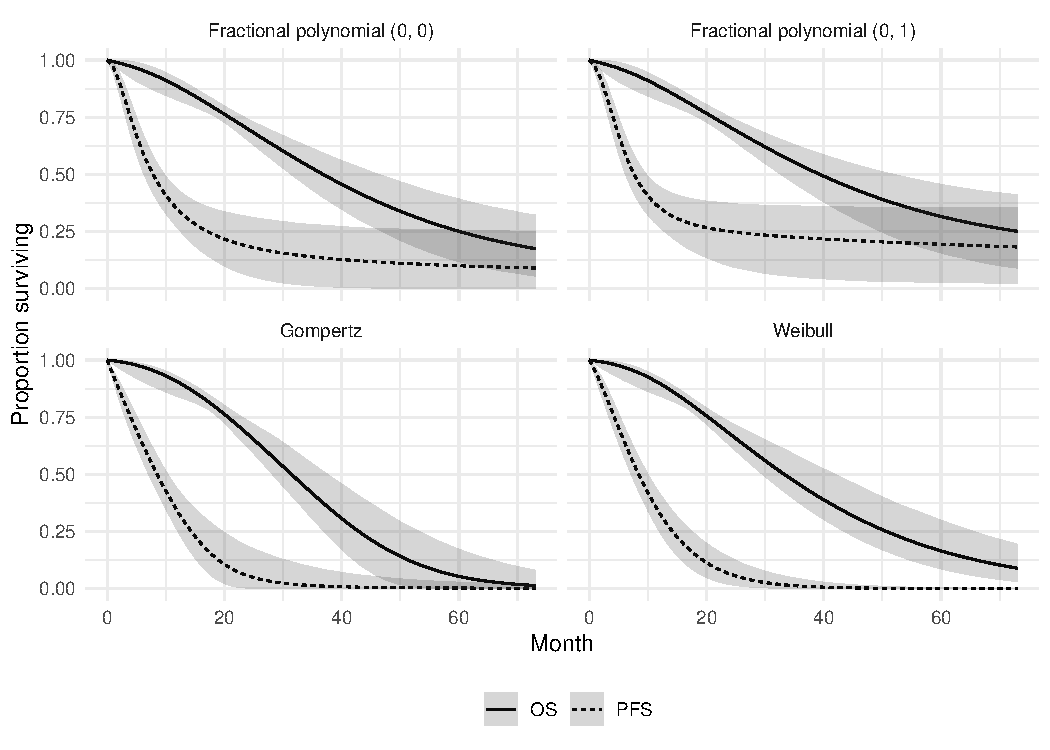
\includegraphics[max size={.8\textwidth}{.8\textheight}]{figs/surv-2L-t790m-osi.pdf}
\caption{Osimertinib among T790M positive patients} \label{subfig:surv-2L_t790m-osi}
\end{subfigure}
\caption{Second line estimates of progression-free survival and overall survival from the multi-state meta-analysis}\label{fig:surv-2L}
\begin{minipage}{\linewidth}
\footnotesize
Notes: The simulated posterior distribution of the parameters of the Bayesian multi-state NMA was used to simulate a distribution of progression-free survival and overall survival curves. The solid lines are posterior means and the shaded region denotes the 95 percent credible interval.
\end{minipage}
\end{figure}

\subsubsection{Software}
The parameters of the different models were estimated using a Markov Chain Monte Carlo (MCMC) method implemented in the JAGS software package. All JAGS analyses were run using \R{} statistical software \citep{team2014r}.

\subsubsection{Use of meta-analysis results in economic model}
Informed by model fit criteria, we used treatment effect estimates obtained with the fixed and random effects, Weibull and fractional polynomial models without a treatment effect for progression to death for the economic model.  When a 3-state economic model is used, the 1L NMA is used to directly simulate disease progression. However, if a 4-state model is used, then both 1L and 2L estimates are incorporated. In particular, the 1L results are used to simulate the transition from $S_1$ to $P_1 \rightarrow S_2$ and the 2L results are used to simulate the transition from $P_1 \rightarrow S_2$ to $P_2$, $P_2$ to $D$, and $P_1 \rightarrow S_2$ to $D$ (see \autoref{fig:model-structure-4-states}). 




\subsection{Adverse events}\label{subsec:data-aes}
The identified RCTs also provided the evidence base to estimate treatment specific adverse eent probabilities. Since adverse events in nearly all RCTs were reported as the number of patients experiencing the event, the NMA was performed on the proportion of patients experiencing the event of interest with a binomial likelihood and logit link \citep[Chapter~2]{dias2018network}. \hl{Add details about pooling and the priors...}

\subsection{Utilities}\label{subsec:data-utility}
Health state utilities based on public literature are reported in \autoref{tbl:state-utility}. We assume that utilities do not vary across treatment strategies. We use estimates from \citet{nafees2017health}, a global study of patients with metastatic NSCLC that used health states representative of 1L treatment to derive utility values. Estimates are based on the "global" analysis that pooled estimates across 6 countries (Australia, China, France, Korea, Taiwan, and the UK) for patients with stable disease and no side effects. Utilities for patients with progressed disease are based on \citet{nafees2008health}, a study representative of metastatic NSCLC patients on 2L treatment. Estimates are from predictions using the mixed model among patients with no adverse events. Utility in the P1/S2 state is estimated using patients that have not yet progressed while on 2L, while estimates in the P2 state are among the progressed 2L patients. 

\begin{table}[!ht]
\begin{center}
\begin{threeparttable}
\caption{Utility by health state} \label{tbl:state-utility}
\begin{tabularx}{\textwidth}{@{\extracolsep{\fill}}lrrl}
\hline
\multicolumn{1}{l}{Health state} & \multicolumn{1}{l}{Mean} & \multicolumn{1}{l}{Standard error} & \multicolumn{1}{l}{Reference} \\
\hline
\ExpandableInput{tables/state-utility.txt}
\hline
\end{tabularx}
\scriptsize
\end{threeparttable}
\end{center}
\end{table}

Adverse even disutilities are displayed in \autoref{tbl:ae-disutility}. When we cannot identify a disutility for an adverse event, we assume that the disutility is equivalent to the disutility from the "most similar" adverse event. Elevated alanine transaminase and elevated aspartate transaminase are assumed to have no effect on utility since they are based on test results and are not medical conditions.      

\begin{table}[!ht]
\begin{center}
\begin{threeparttable}
\caption{Disutility due to adverse events} \label{tbl:ae-disutility}
\begin{tabularx}{\textwidth}{@{\extracolsep{\fill}}lrrl}
\hline
\multicolumn{1}{l}{Adverse event} & \multicolumn{1}{l}{Mean} & \multicolumn{1}{l}{Standard error} & \multicolumn{1}{l}{Reference} \\
\hline
\ExpandableInput{tables/ae-disutility.txt}
\hline
\end{tabularx}
\scriptsize
\end{threeparttable}
\end{center}
\end{table}

\subsection{Health care sector costs}\label{subsec:data-costs}
\subsubsection{Treatment costs}
Treatment costs are a function of drug acquisition and drug administration costs. Dosage for each drug based on Federal Drug Administration (FDA) labels is presented in \autoref{tbl:dosage}. Patients using PBDC are, by default, assumed to use a combination of cisplatin and pemetrexed, although this can be adjusted in the \pkg{R} package. At a given treatment line, patients continue to take a drug until disease progression or the end of a treatment cycle. For example, a patient using erlotinib at 1L would take a 150 mg tablet each day until disease progression, at which point they would begin to use the 2L drug. Conversely, a patient using PBDC at 2L would discontinue cisplatin and pemetrexed after completing 6 21-day cycles. 

\begin{table}[!ht]
\begin{center}
\begin{threeparttable}
\caption{Drug dosage} \label{tbl:dosage}
\begin{tabularx}{\textwidth}{@{\extracolsep{\fill}}lp{0.7\linewidth}}
\hline
\multicolumn{1}{l}{Drug} & \multicolumn{1}{l}{Dosage} \\
\hline
\ExpandableInput{tables/dosage.txt}
\hline
\end{tabularx}
\scriptsize
\end{threeparttable}
\end{center}
\end{table}

In some cases, patients might be required to use multiple dosage forms to obtain the recommended dosage. In these cases, we assume that patients use the cheapest possible combination of dosage forms. For instance, dosage for nivolumab is 240 mg every 2 weeks, so patients are assumed to use 2 100mg vials and 1 40mg vials. 

Dosing with cisplatin depends on body weight. The mean body surface area (BSA) in the United States is $1.6m^2$ for women and $1.9m^2$ for men, which implies a dose of of 120 mg for women of and 142.5 mg for men. The model assumes that there is no vial sharing, so patients use 1 100mg vial and 1 50 mg vial of cisplatin.  

Wholesale acquisition costs (WACs) are shown in \autoref{tbl:acq-costs}. Drug acquisition costs in the model are equal to the WACs adjusted for discounts and rebates. These discounts can be applied to uniquely to each drug in the \pkg{R} package, but are, by default, assumed to range from 20\% to 30\%. When historical data was available, we used the most recently available WAC from either ProspectoRx or AnalySource. There was no historical data for dacomitinib, so we used the publicly announced WAC of \$12,400 per month.  

\begin{table}[!ht]
\begin{center}

\begin{threeparttable}
\caption{Wholesale acquisition costs} \label{tbl:acq-costs}
\begin{tabularx}{\textwidth}{@{\extracolsep{\fill}}llr}
\hline
\multicolumn{1}{l}{Drug} & \multicolumn{1}{l}{Strength} & \multicolumn{1}{l}{Acquisition cost} \\
\hline
\ExpandableInput{tables/acq_costs.txt}
\hline
\end{tabularx}
\scriptsize
\end{threeparttable}
\end{center}
\end{table}

\autoref{tbl:admin-costs} reports drug administration costs. Drug administration costs are based on US Current Procedures Terminology (CPT) codes and accrued each time a patient takes a drug. 

\begin{table}[!ht]
\begin{center}
\begin{threeparttable}
\caption{Drug administration costs} \label{tbl:admin-costs}
\begin{tabularx}{\textwidth}{@{\extracolsep{\fill}}lrl}
\hline
\multicolumn{1}{l}{Drug} & \multicolumn{1}{l}{Administration cost} & \multicolumn{1}{l}{Source} \\
\hline
\ExpandableInput{tables/admin_costs.txt}
\hline
\end{tabularx}
\scriptsize
\end{threeparttable}
\end{center}
\end{table}

\subsubsection{Inpatient and outpatient costs}

\begin{table}[!ht]
\begin{center}
\begin{threeparttable}
\caption{Monthly inpatient medical costs} \label{tbl:inpt-costs}
\begin{tabularx}{\textwidth}{@{\extracolsep{\fill}}lrrl}
\hline
\multicolumn{1}{c}{Health state} & \multicolumn{1}{l}{Mean} & \multicolumn{1}{l}{Standard error} & \multicolumn{1}{l}{Reference}  \\
\hline
\ExpandableInput{tables/inpt_costs.txt}
\hline
\end{tabularx}
\scriptsize
\end{threeparttable}
\end{center}
\end{table}

\begin{table}[!ht]
\begin{center}
\begin{threeparttable}
\caption{Monthly outpatient medical costs} \label{tbl:op-costs}
\begin{tabularx}{\textwidth}{@{\extracolsep{\fill}}lrrl}
\hline
\multicolumn{1}{c}{Health state} & \multicolumn{1}{l}{Mean} & \multicolumn{1}{l}{Standard error} & \multicolumn{1}{l}{Reference}  \\
\hline
\ExpandableInput{tables/op_costs.txt}
\hline
\end{tabularx}
\scriptsize
\end{threeparttable}
\end{center}
\end{table}


\subsubsection{Adverse event costs}
\begin{table}[!ht]
\begin{center}
\begin{threeparttable}
\caption{Costs of adverse events} \label{tbl:ae-costs}
\begin{tabularx}{\textwidth}{@{\extracolsep{\fill}}lrrrl}
\hline
\multicolumn{1}{c}{Adverse event} & \multicolumn{1}{l}{Mean} & \multicolumn{1}{l}{Lower} &  \multicolumn{1}{l}{Upper} & \multicolumn{1}{l}{Reference}  \\
\hline
\ExpandableInput{tables/ae_costs.txt}
\hline
\end{tabularx}
\scriptsize
\end{threeparttable}
\end{center}
\end{table}


\subsection{Productivity}\label{subsec:data-productivity}
Productivity costs are currently estimated using the human capital approach (HCA), which measures lost productivity using work time lost. The approach is rooted in economic theory as time away from work is valued at the market wage, which, in a competitive market, reflects the societal value of work. The HCA contrasts with the friction cost approach (FCA), which only measures productivity losses during the time (i.e., the friction period) required to replace workers leaving employment due to illness. A practical limitation of the FCA is that it is difficult to reliably estimate the friction period, which depends on the unemployment rate and consequently varies considerably across individuals and over time. In general, the HCA tends to overestimate productivity losses while the FCA may underestimate them. 

Similar to \citet{hanly2012breast}, time lost from work in the model stems from three sources: temporary disability, permanent disability, and premature death. Temporary disability is measured using the mean duration of absence from work due to sick leave. A central estimate from the literature of the number of missed work days due to cancer is $\MissedDaysEst$ \citep{mehnert2011employment}, which we, by default, vary by 20\% in either direction in the PSA. Permanent disability is measured as the average reduction in work hours among cancer survivors. \citet{short2008long} estimate an average reduction of $\HoursReductionLower$ to $\HoursReductionUpper$ hours per week, which is inclusive of survivors who stopped working completely and similar across males and females. Work lost from premature mortality is the time from death (within the simulation) until retirement age (age 65). 

Wages stratified by gender and employment status are reported in \autoref{tbl:wages}. Estimates of both the weekly wage and the proportion of individuals by employment status are from the U.S. Bureau of Labor Statistics. Productivity costs are computed by multiplying time lost from work (in weeks) by the weekly wage. 

\begin{table}[!ht]
\begin{center}
\begin{threeparttable}
\caption{Weekly wages by gender and employment status} \label{tbl:wages}
\begin{tabularx}{\textwidth}{@{\extracolsep{\fill}}lrr}
\hline
 \multicolumn{1}{l}{Employment status} & \multicolumn{1}{l}{Percentage} &  \multicolumn{1}{l}{Weekly wage} \\
\hline
 \multicolumn{3}{c}{\textit{Women}}\\
\ExpandableInput{tables/wages_female.txt} \\
 \multicolumn{3}{c}{\textit{Men}}\\
\ExpandableInput{tables/wages_male.txt}
\hline
\end{tabularx}
\scriptsize
\end{threeparttable}
\end{center}
\end{table}


\subsection{Value of hope}\label{subsec:data-voh}
As described in more detail in \autoref{app:value-of-hope}}, the value of hope depends on the form of the utility function and the estimate of relative risk aversion. Following \citet{shafrin2017patient}, we use the constant relative risk aversion utility function $u(x) = x^\eta$ where $\eta = 1.39$, which was estimated among patients with NSCLC. 

\section{Simulation and uncertainty analysis}\label{sec:uncertainty-analysis}
\subsection{Parameter uncertainty} \label{subsec:psa}
Parameter uncertainty is quantified using probabilistic sensitivity analysis (PSA), which propagates uncertainty in the model input parameters throughout the model by randomly sampling the input parameters from suitable probability distributions \citep{baio2015probabilistic}, \citep{claxton2005probabilistic}.Probability distributions are determined according to the distributional properties of the statistical estimates, which, in turn, depend on the statistical techniques used, and the distributions of the underlying data. \autoref{tbl:psa-distributions} displays the probability distribution that we used for the model parameters. When conducting a CEA, the results of the PSA are summarized using standard measures from the literature including cost-effectiveness planes, cost-effectiveness acceptability curves, and estimates of the expected value of perfect information \citep{black1990plane}, \citep{van1994costs}, \citep{briggs1999bayesian}. Furthermore, all point estimates from a CEA or MCDA are reported along with 95 percent confidence intervals. 

\begin{table}[!ht]
\begin{center}
\begin{threeparttable}
\caption{Probability distributions for probabilistic sensitivity analysis} \label{tbl:psa-distributions}
\begin{tabular}{p{0.5\linewidth}p{0.5\linewidth}}
\hline
\multicolumn{1}{l}{Parameter(s)} & \multicolumn{1}{l}{Distribution}\\
\hline
\multicolumn{2}{@{}l}{\textbf{Health state transitions}} \\
Bayesian multi-state NMA & Simulated posterior distribution\\
&\\
\multicolumn{2}{@{}l}{\textbf{Adverse events}} \\
Bayesian NMA for adverse events & Simulated posterior distribution\\
&\\
\multicolumn{2}{@{}l}{\textbf{Utility}} \\
Health state utility & Normal\\
&\\

Adverse event disutilities & Normal\\
&\\
\multicolumn{2}{@{}l}{\textbf{Health care sector costs}} \\
Drug acquisition and administration cost & Fixed \\
&\\
Discounts and rebates applied to drug acquisition cost & Uniform \\
&\\
Inpatient costs & Gamma \\
&\\
Outpatient costs & Gamma \\
&\\
Adverse event costs & Normal\\
&\\
\multicolumn{2}{@{}l}{\textbf{Productivity costs}} \\
Missed work days & Uniform\\
&\\
Reduction in hours worked & Uniform\\


\hline
\end{tabular}
\scriptsize
\end{threeparttable}
\end{center}
\end{table}

\subsection{Structural uncertainty}
Health state probabilities are typically very sensitive to the parametric distributions used in a survival models. We explore this sensitivity by providing options to choose from a number of different distributions. As discussed in \autoref{subsec:data-transprobs} these included the Weibull, Gompertz, and two second order fractional polynomial models $\{(p_0, p_1) = (0, 0), (0,1)\}$. 
Furthermore, both  4-state (\autoref{fig:model-structure-4-states}) and 3-state (\autoref{fig:model-structure-3-states}) model structures can be used. [Need to add detail.]


\subsection{Implementation} 
The individual-level CTSTM was implemented using the R package \href{https://innovationvalueinitiative.github.io/hesim/}{\pkg{hesim}} developed by IVI. The package provides a general framework for integrating parameter estimates from a statistical model with different types of simulation models for economic evaluation. Parameter uncertainty is propagated throughout \textit{hesim} models using PSA. Specifically, we randomly drew all input parameters as described in \autoref{subsec:psa} and simulated the CTSTM for each randomly sampled parameter set. All computationally intensive steps in \pkg{hesim} simulation models are written in C++ so the simulations are fast enough to be run with a PSA in web applications.

\begin{appendices}
\setcounter{table}{0}
\renewcommand{\thetable}{A\arabic{table}}
\setcounter{figure}{0}
\renewcommand{\thefigure}{A\arabic{figure}}
\setcounter{equation}{0}
\renewcommand{\theequation}{A\arabic{equation}}

\section{Systematic Literature Review}\label{app:slr}

\subsection{Treatment effects for transition rates}
Details regarding eligibility criteria defining the scope of the studies considered relevant are outlined in \autoref{tbl:picos-tx-effects-1L}, \autoref{tbl:picos-tx-effects-2L}, and \autoref{tbl:picos-tx-effects-2LP}. 


\begin{table}[!ht]
\begin{center}
\begin{threeparttable}
\caption{PICOS criteria for review of treatment effects (metastatic 1L population)} \label{tbl:picos-tx-effects-1L}
\begin{tabular}{p{0.3\linewidth}p{0.7\linewidth}}
\hline
\multicolumn{1}{l}{PICOS} &  \multicolumn{1}{l}{Criteria}\\
\hline
Population & Adult patients with metastatic non-squamous NSCLC who are EGFR positive and without prior treatment for their disease.\\
&\\
Interventions & The following drugs as monotherapy or in combination with other drugs 
\begin{itemize}
\item erlotinib
\item afatinib
\item gefitinib
\item osimertinib
\item dacomitinib
\end{itemize} \\
Comparators & 
\begin{itemize}
\item placebo
\item best supportive care (BSC), defined as whichever therapy was judged to be appropriate by the treating physician.
\item any intervention of interest
\item any treatment that facilitates an indirect comparison
\end{itemize} \\
Outcomes & 
\begin{itemize}
\item OS
\item PFS
\item TTP
\end{itemize} \\
Study design & RCTs \\
&\\
Other & English language\\
\hline
\end{tabular}
\scriptsize Note: Trials where the overall study population is an all-comer population, but subgroup results are reported for the target population of interest are included. A trial or subgroup where the study population is a mixture of non-squamous and squamous patients is included if over 90\% is non-squamous. 
\end{threeparttable}
\end{center}
\end{table}


\begin{table}[!ht]
\begin{center}
\begin{threeparttable}
\caption{PICOS criteria for review of treatment effects (metastatic 2L population)} \label{tbl:picos-tx-effects-2L}
\begin{tabular}{p{0.3\linewidth}p{0.7\linewidth}}
\hline
\multicolumn{1}{l}{PICOS} &  \multicolumn{1}{l}{Criteria}\\
\hline
Population & Adult patients with metastatic non-squamous NSCLC who are EGFR+ positive and
who have experienced progression after one line of prior treatment.\\
&\\
Interventions & The following drugs as monotherapy or in combination with other drugs 
\begin{itemize}
\item erlotinib
\item afatinib
\item gefitinib
\item osimertinib
\item dacomitinib
\item nivolumab
\item pembrolizumab
\item atezolizumab
\item bevacizumab
\item platinum-based doublet therapy
\end{itemize} \\
Comparators & 
\begin{itemize}
\item placebo
\item best supportive care (BSC), defined as whichever therapy was judged to be appropriate by the treating physician.
\item any intervention of interest
\item any treatment that facilitates an indirect comparison
\end{itemize} \\
Outcomes & 
\begin{itemize}
\item OS
\item PFS
\item TTP
\end{itemize} \\
Study design & RCTs \\
&\\
Other & English language\\
\hline
\end{tabular}
\scriptsize Note: Trials where the overall study population is an all-comer population, but subgroup results are reported for the target population of interest are included. A trial or subgroup where the study population is a mixture of non-squamous and squamous patients is included if over 90\% is non-squamous.  
\end{threeparttable}
\end{center}
\end{table}

\begin{table}[!ht]
\begin{center}
\begin{threeparttable}
\caption{PICOS criteria for review of treatment effects (metastatic 2L+ population)} \label{tbl:picos-tx-effects-2LP}
\begin{tabular}{p{0.3\linewidth}p{0.7\linewidth}}
\hline
\multicolumn{1}{l}{PICOS} &  \multicolumn{1}{l}{Criteria}\\
\hline
Population & Adult patients with metastatic non-squamous NSCLC who are EGFR+ positive and
who have experienced progression after two or more prior prior treatments.\\
&\\
Interventions & The following drugs as monotherapy or in combination with other drugs 
\begin{itemize}
\item nivolumab
\item pembrolizumab
\item atezolizumab
\item bevacizumab
\item platinum-based doublet therapy
\end{itemize} \\
Comparators & 
\begin{itemize}
\item placebo
\item best supportive care (BSC), defined as whichever therapy was judged to be appropriate by the treating physician.
\item any intervention of interest
\item any treatment that facilitates an indirect comparison
\end{itemize} \\
Outcomes & 
\begin{itemize}
\item OS
\item PFS
\item TTP
\end{itemize} \\
Study design & RCTs \\
&\\
Other & English language\\
\hline
\end{tabular}
\scriptsize Note: Trials where the overall study population is an all-comer population, but subgroup results are reported for the target population of interest are included. A trial or subgroup where the study population is a mixture of non-squamous and squamous patients is included if over 90\% is non-squamous.  
\end{threeparttable}
\end{center}
\end{table}



\subsection{Utilities}
Health state utility values (EQ-5d, HUI2, HUI-3, SF-6D) for the different health states were used in the model as well as disutility estimates associated with adverse events identified by focusing on review or overview studies. Furthermore, published mapping algorithms that allow a non-preference-based measure (generic or disease-specific measure) to be mapped onto a generic preference-based measure are of interest, as well as mapping algorithms between different generic preference-based health state utility values (e.g. between SF-6D and EQ5D) will be searched for. See Appendix Table 4 for study selection criteria.

\subsection{Resource use, productivity, and cost}
Relevant evidence regarding resource use, productivity and cost estimates were identified by means of a review of published CEA modelling studies in NSCLC relevant for the US setting.  See Appendix Table 5 for study selection criteria.

\subsection{Study identification}
Relevant studies were identified by searching the following databases using predefined search strategies: Medical Literature Analysis and Retrieval System Online (MEDLINE), Excerpta Medica database (EMBASE), and Cochrane Central Register of Controlled Trials. The study design filters recommended by the Scottish Intercollegiate Guidelines Network (SIGN) for MEDLINE and EMBASE were used to identify clinical trials. The search included terms related to the generic and brand name of the interventions of interest. The US National Institutes of Health Clinical Trial Registry and EU Clinical Trials Registry were also searched to identify completed clinical trials not yet published to identify any completed or ongoing trials that meet the criteria with results available.

For utility studies, and CEA studies providing evidence on healthcare utilization and costs, the following additional databases were searched in addition: NHS Economic Evaluation Database (NHS EED), Health Economic Evaluations Database (HEED), THe Health Economics Research Centre-maintained mapping algorithm database, and The University of Sheffield's ScHARRHUD database of health utilities' evidence.

Where there were gaps in the identified evidence, the search was expanded to include the grey literature, such as reports published by NICE.

\subsection{Study selection}
Two reviewers, working independently, reviewed all abstracts and proceedings identified in each of the searches according to the selection criteria, with the exception of outcome criteria in the efficacy and safety searches, which were only applied during the screening of full-text publications. All studies identified as eligible studies during abstract screening were then screened at a full-text stage by the same two reviewers. The full-text studies identified at this stage were included for data extraction. Following reconciliation between the two investigators, a third reviewer was included to reach consensus for any remaining discrepancies. The process of study identification and selection is summarized with Preferred Reporting Items for Systematic Reviews and Meta-Analyses (PRISMA) flow diagrams (including reasons for exclusion at both the abstract and full text screening stage). 

\subsection{Data collection}
For the clinical studies, two reviewers, working independently, extracted data on study characteristics, interventions, patient characteristics, and outcomes for the final list of included studies. Following reconciliation between the two reviewers, a third reviewer was included to reach consensus on any remaining discrepancies. For all outcomes of interest, information regarding point estimates, variability and uncertainty was obtained. For PFS and OS, hazard ratios and associated information regarding uncertainty were extracted. If results were reported as forest plots, the point estimate and 95\$ percent\ confidence interval were extracted using DigitizeIt software version 2.1.4 (Bormisoft - Informer Technologies, Inc.). Kaplan Meier curves will also be digitzed using DigitizeIt and the proportion of patients free of the event over time will be extracted and the number of patients at risk over time. Adverse events were collected, if reported. Data collected included number and percent of patients with: any grade 3 or 4 adverse event, any grade 3 or 4 treatment related adverse event, any serious adverse event, any treatment related serious adverse event, and death within 30 days of last treatment. The duration over which safety outcomes were reported were also captured. Discontinuation due to adverse events were also examined. 

For utility and cost-effectiveness studies, relevant information for the model was extracted from the source publications and checked by a second-reviewer. 

\subsection{Limitations}
Despite the strengths of the proposed SLR, some limitations are applicable to all SLRs that should be acknowledged. As the evidence base is continually growing, any trials published after the search date will not be captured. Further, any trials that are published close to the search date but are not yet indexed in the databases at the time of the search will not be captured by the search of MEDLINE, EMBASE, and Cochrane Central Register of Controlled Trials. As with any literature review, this SLR is limited by the use of published data. There is a risk of publication bias as some clinical studies fail to be published while others are published only in abstract form, which presents limited information. Finally, the search and selection were restricted to trials published in English.

\section{Network meta-analysis for transition rates}

\subsection{Kaplan-Meier curves}
\iffalse
\begin{figure}
\centering
\begin{subfigure}{\textwidth}
\centering
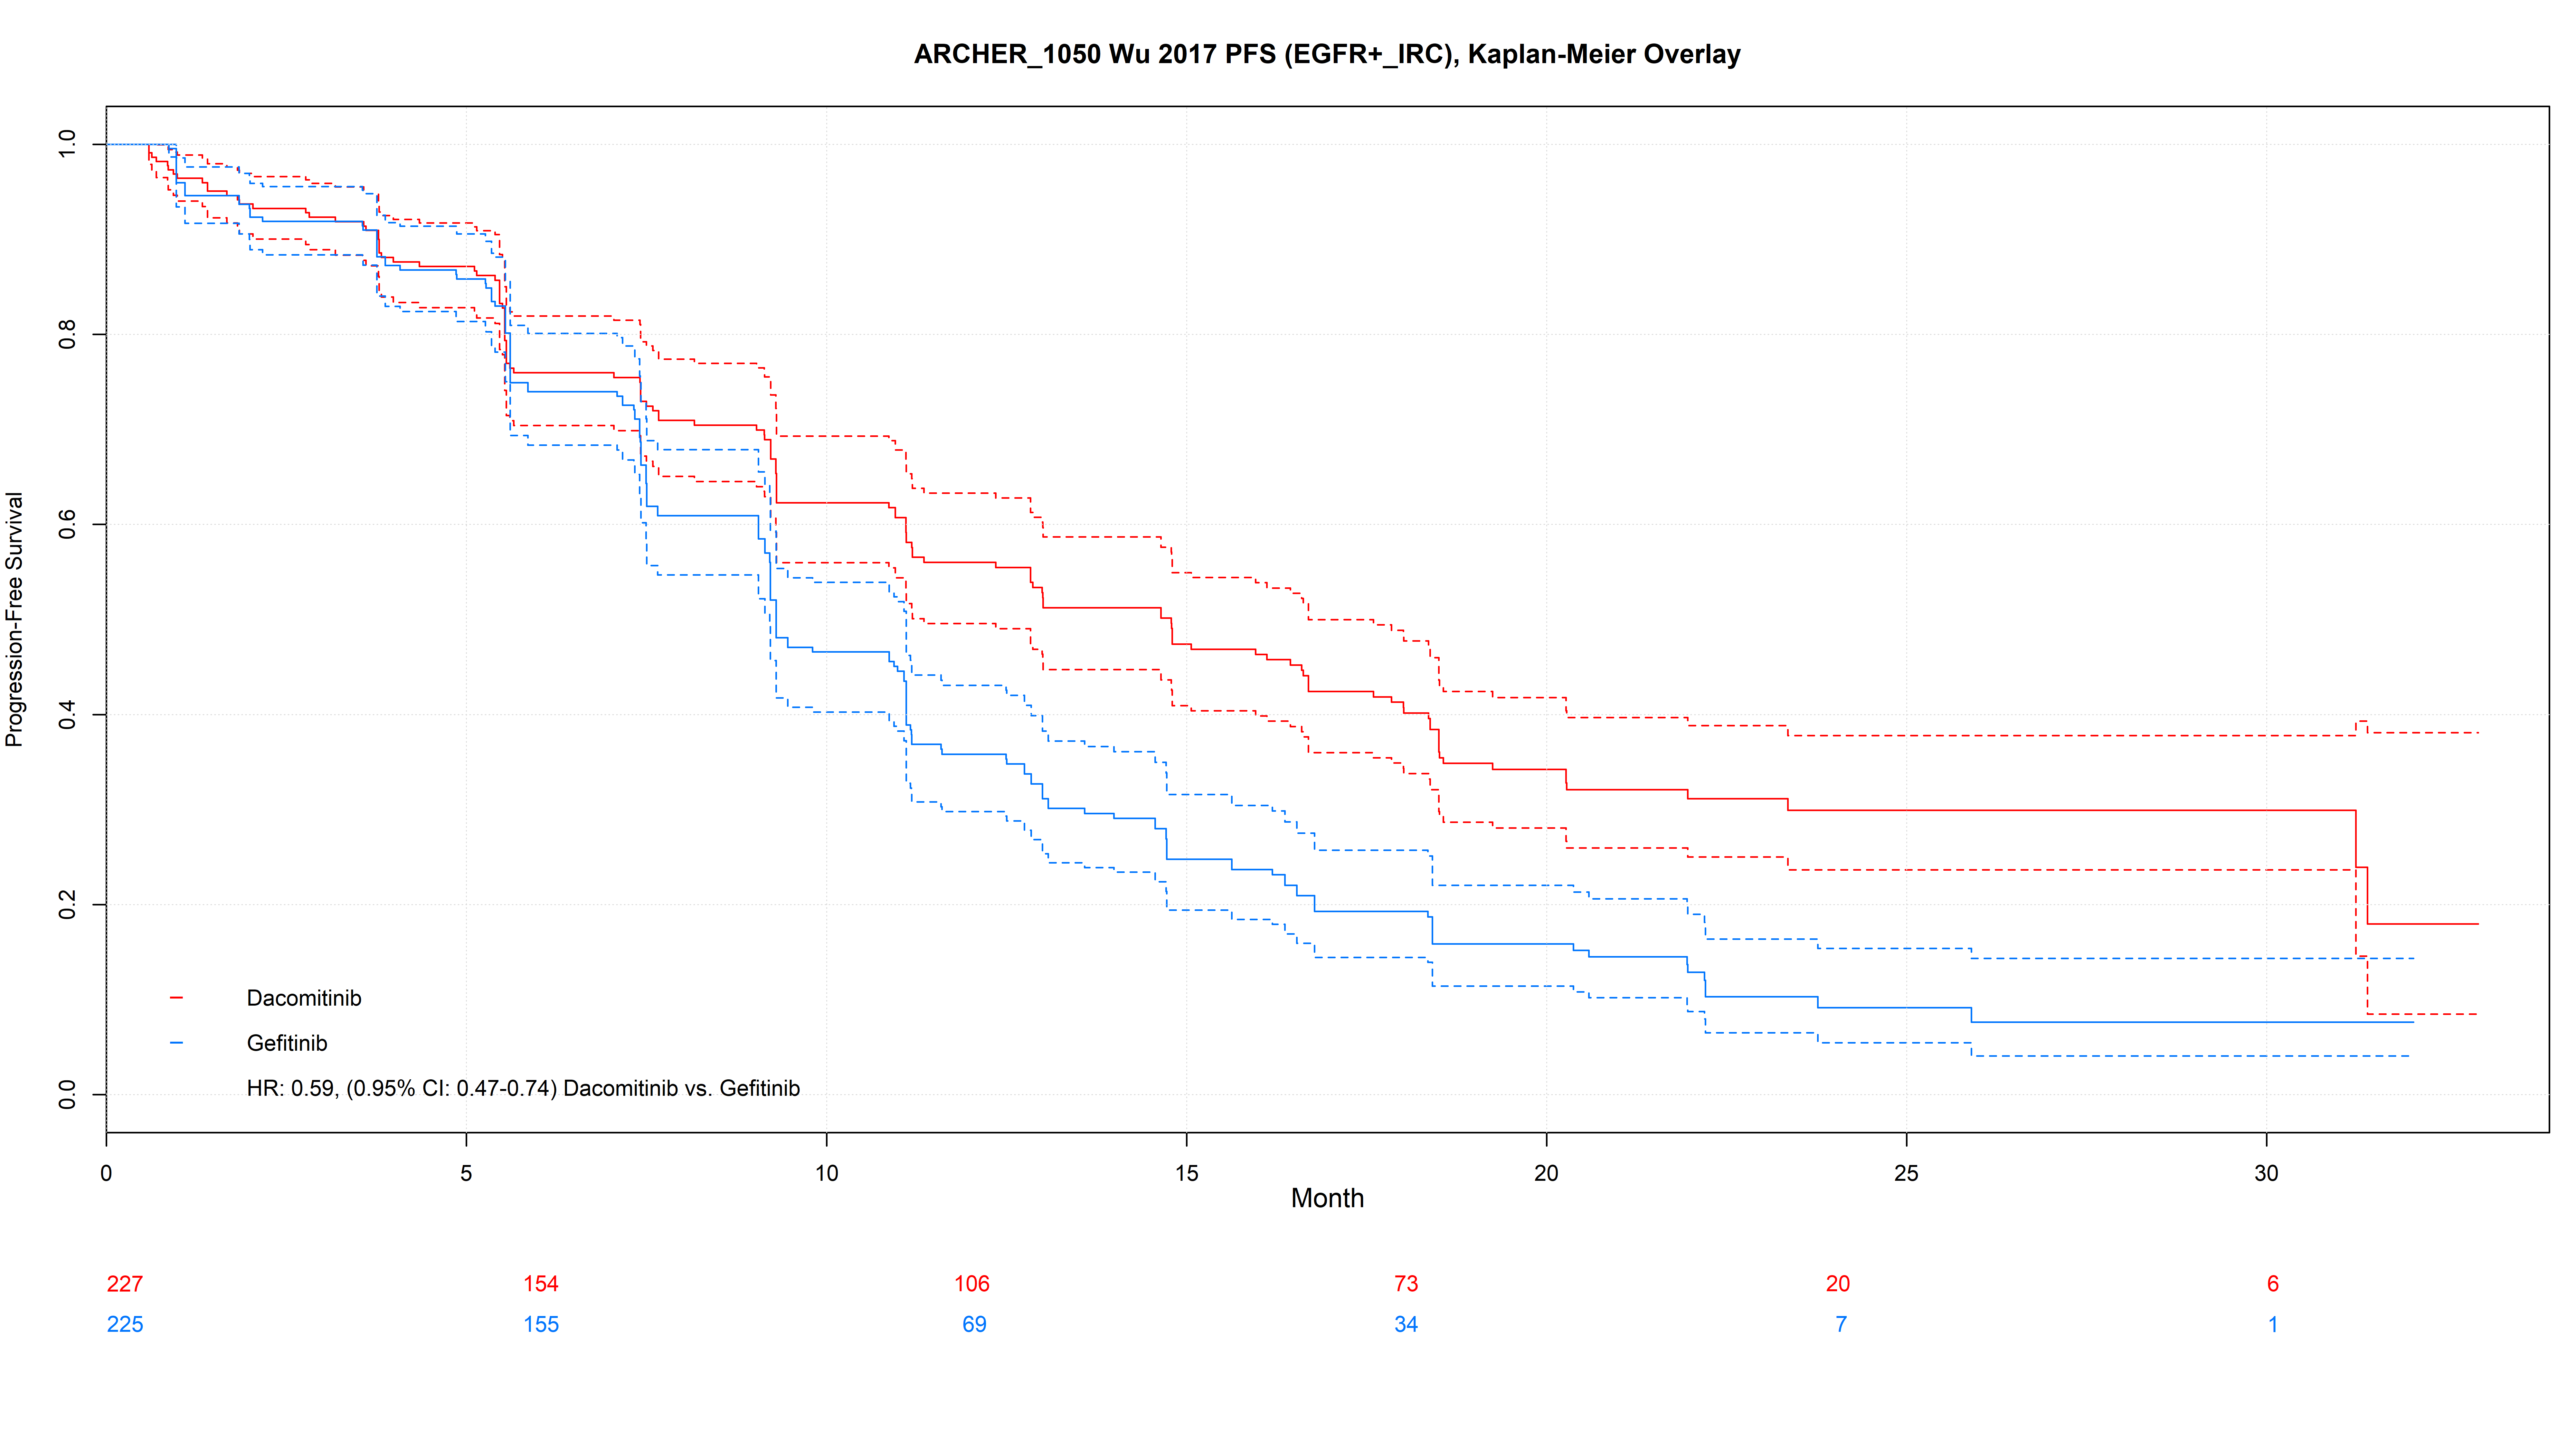
\includegraphics[max size={\textwidth}{\textheight}]{figs/km-plots/ARCHER_1050 Wu 2017 PFS (EGFR+_IRC) Kaplan Meier.png}
\end{subfigure}
\begin{subfigure}{\textwidth}
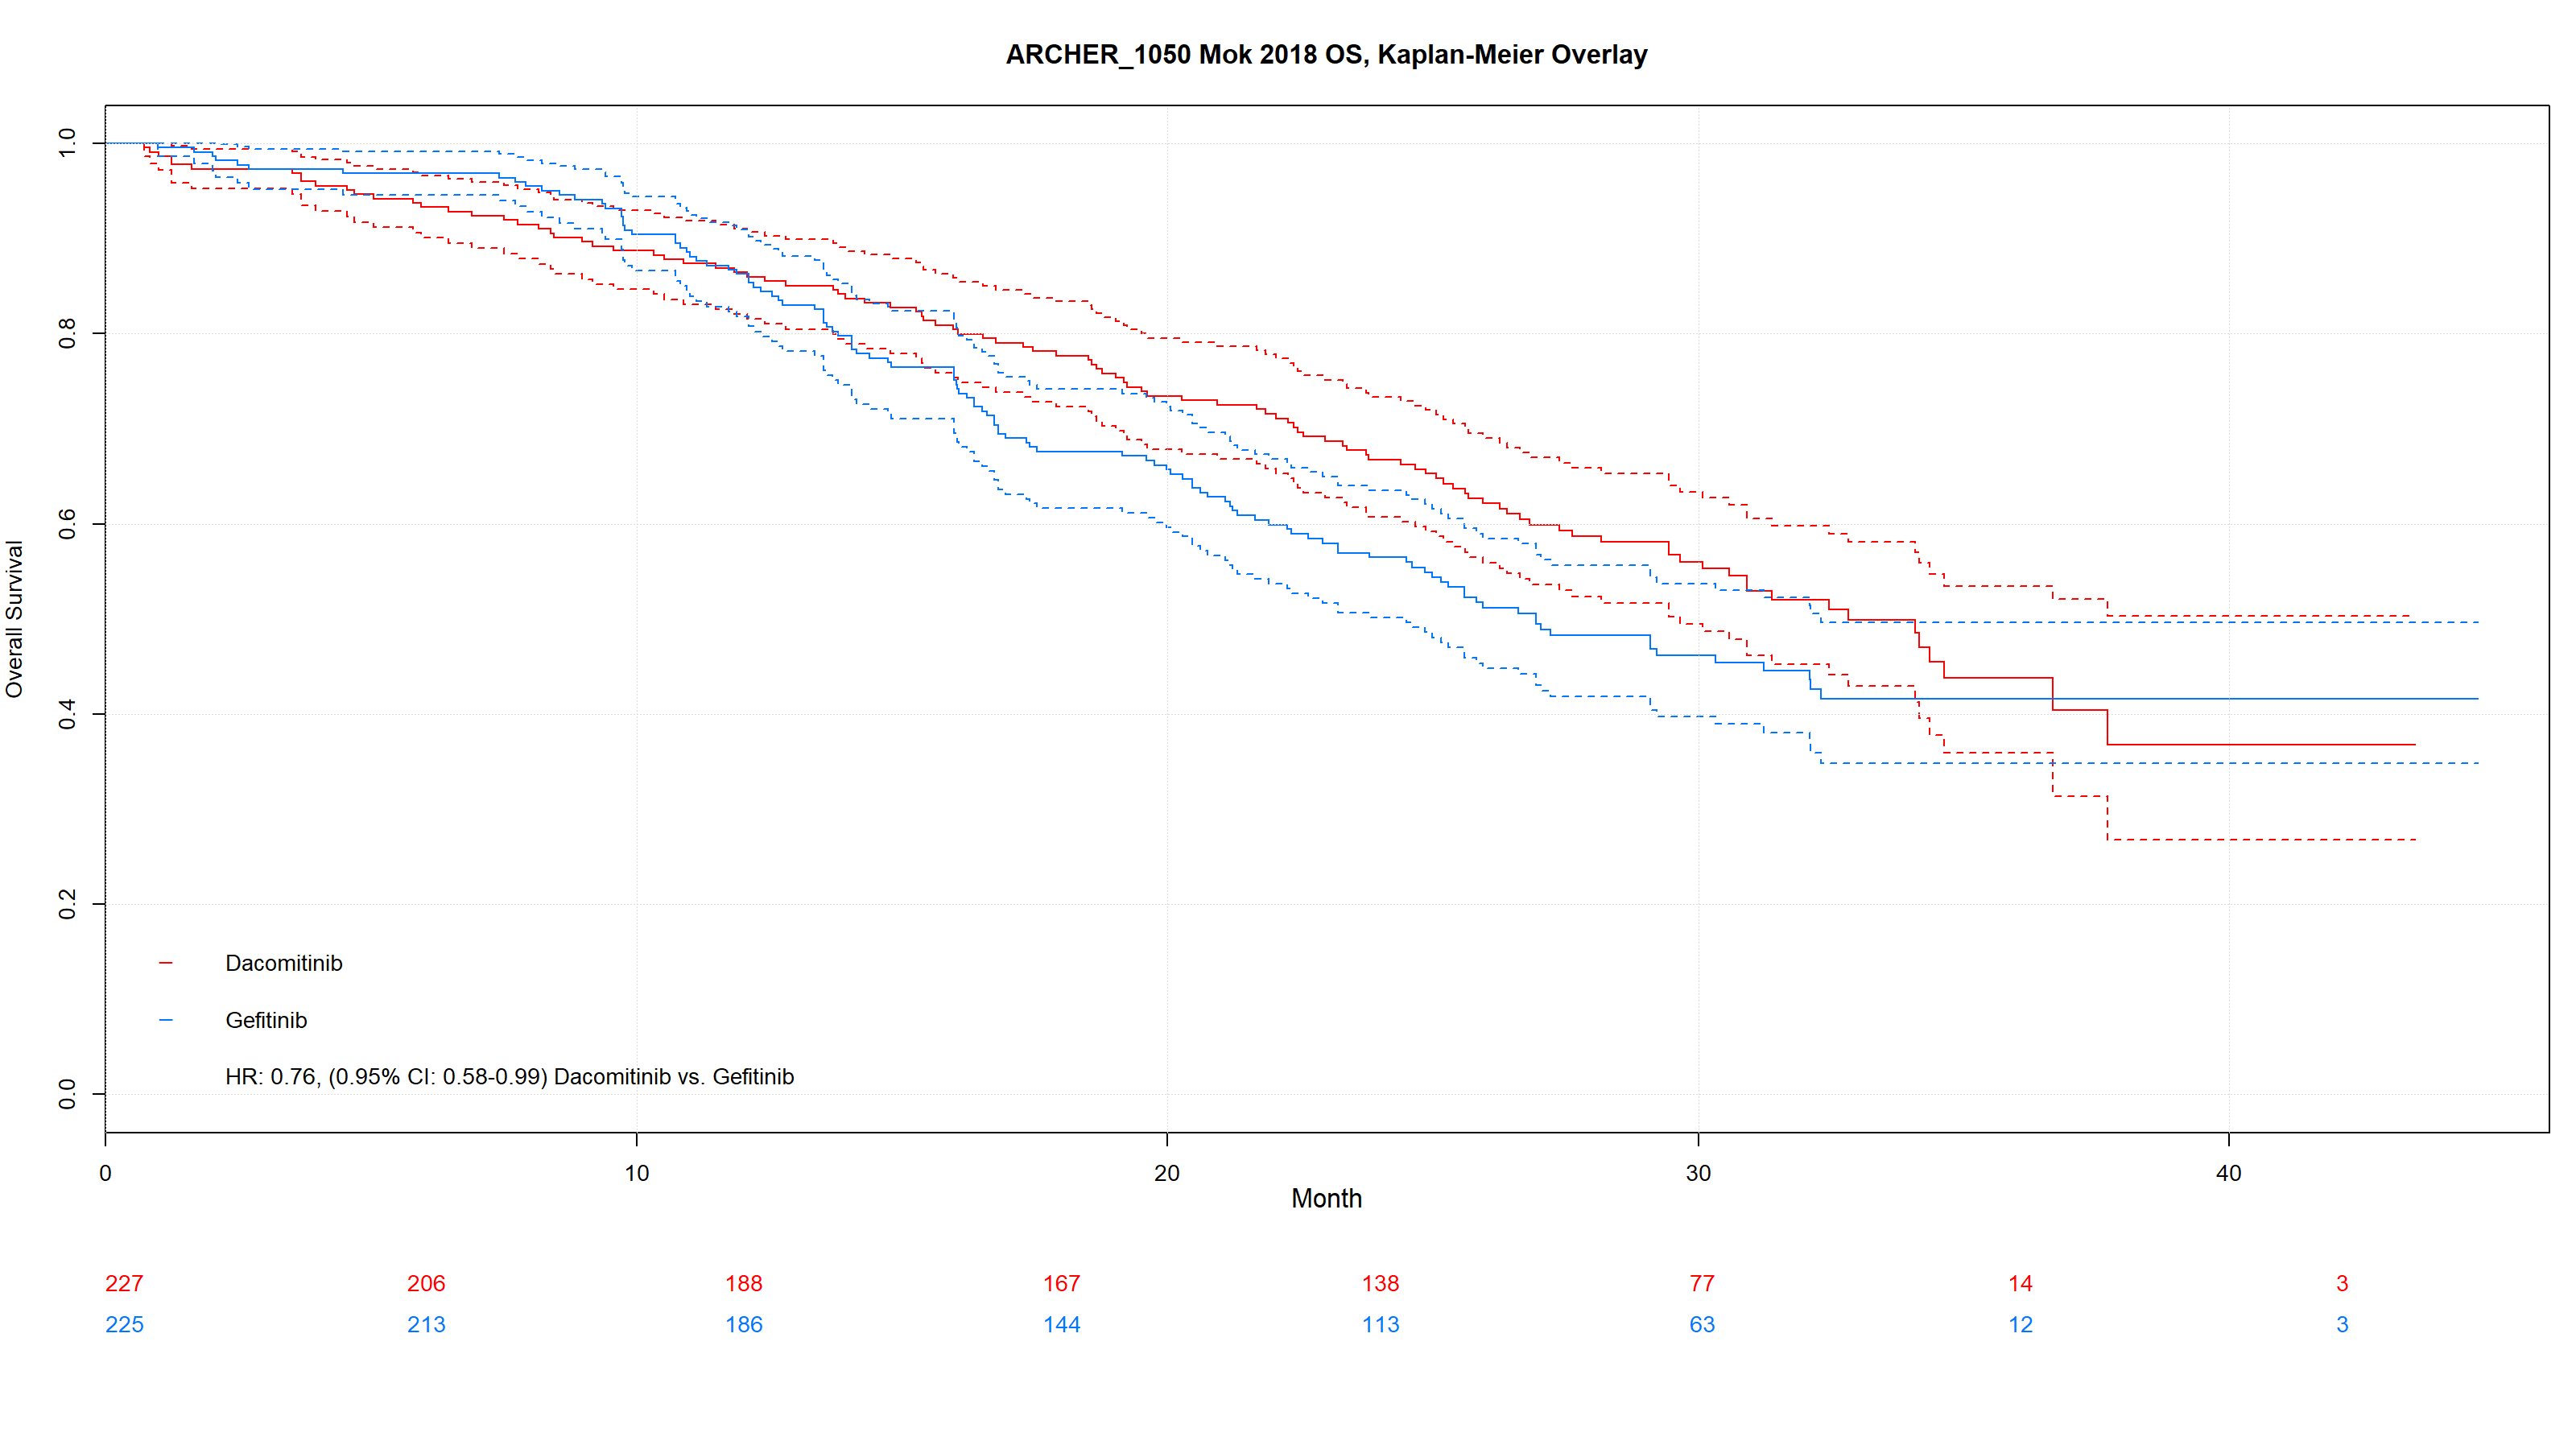
\includegraphics[max size={\textwidth}{\textheight}]{figs/km-plots/ARCHER_1050 Mok 2018 OS Kaplan Meier.png}
\end{subfigure}
\centering
\caption{ARCHER-1050, progression-free survival and overall survival}\label{fig:ARCHER-1050}
\end{figure}


\begin{figure}
\centering
\begin{subfigure}{\textwidth}
\centering
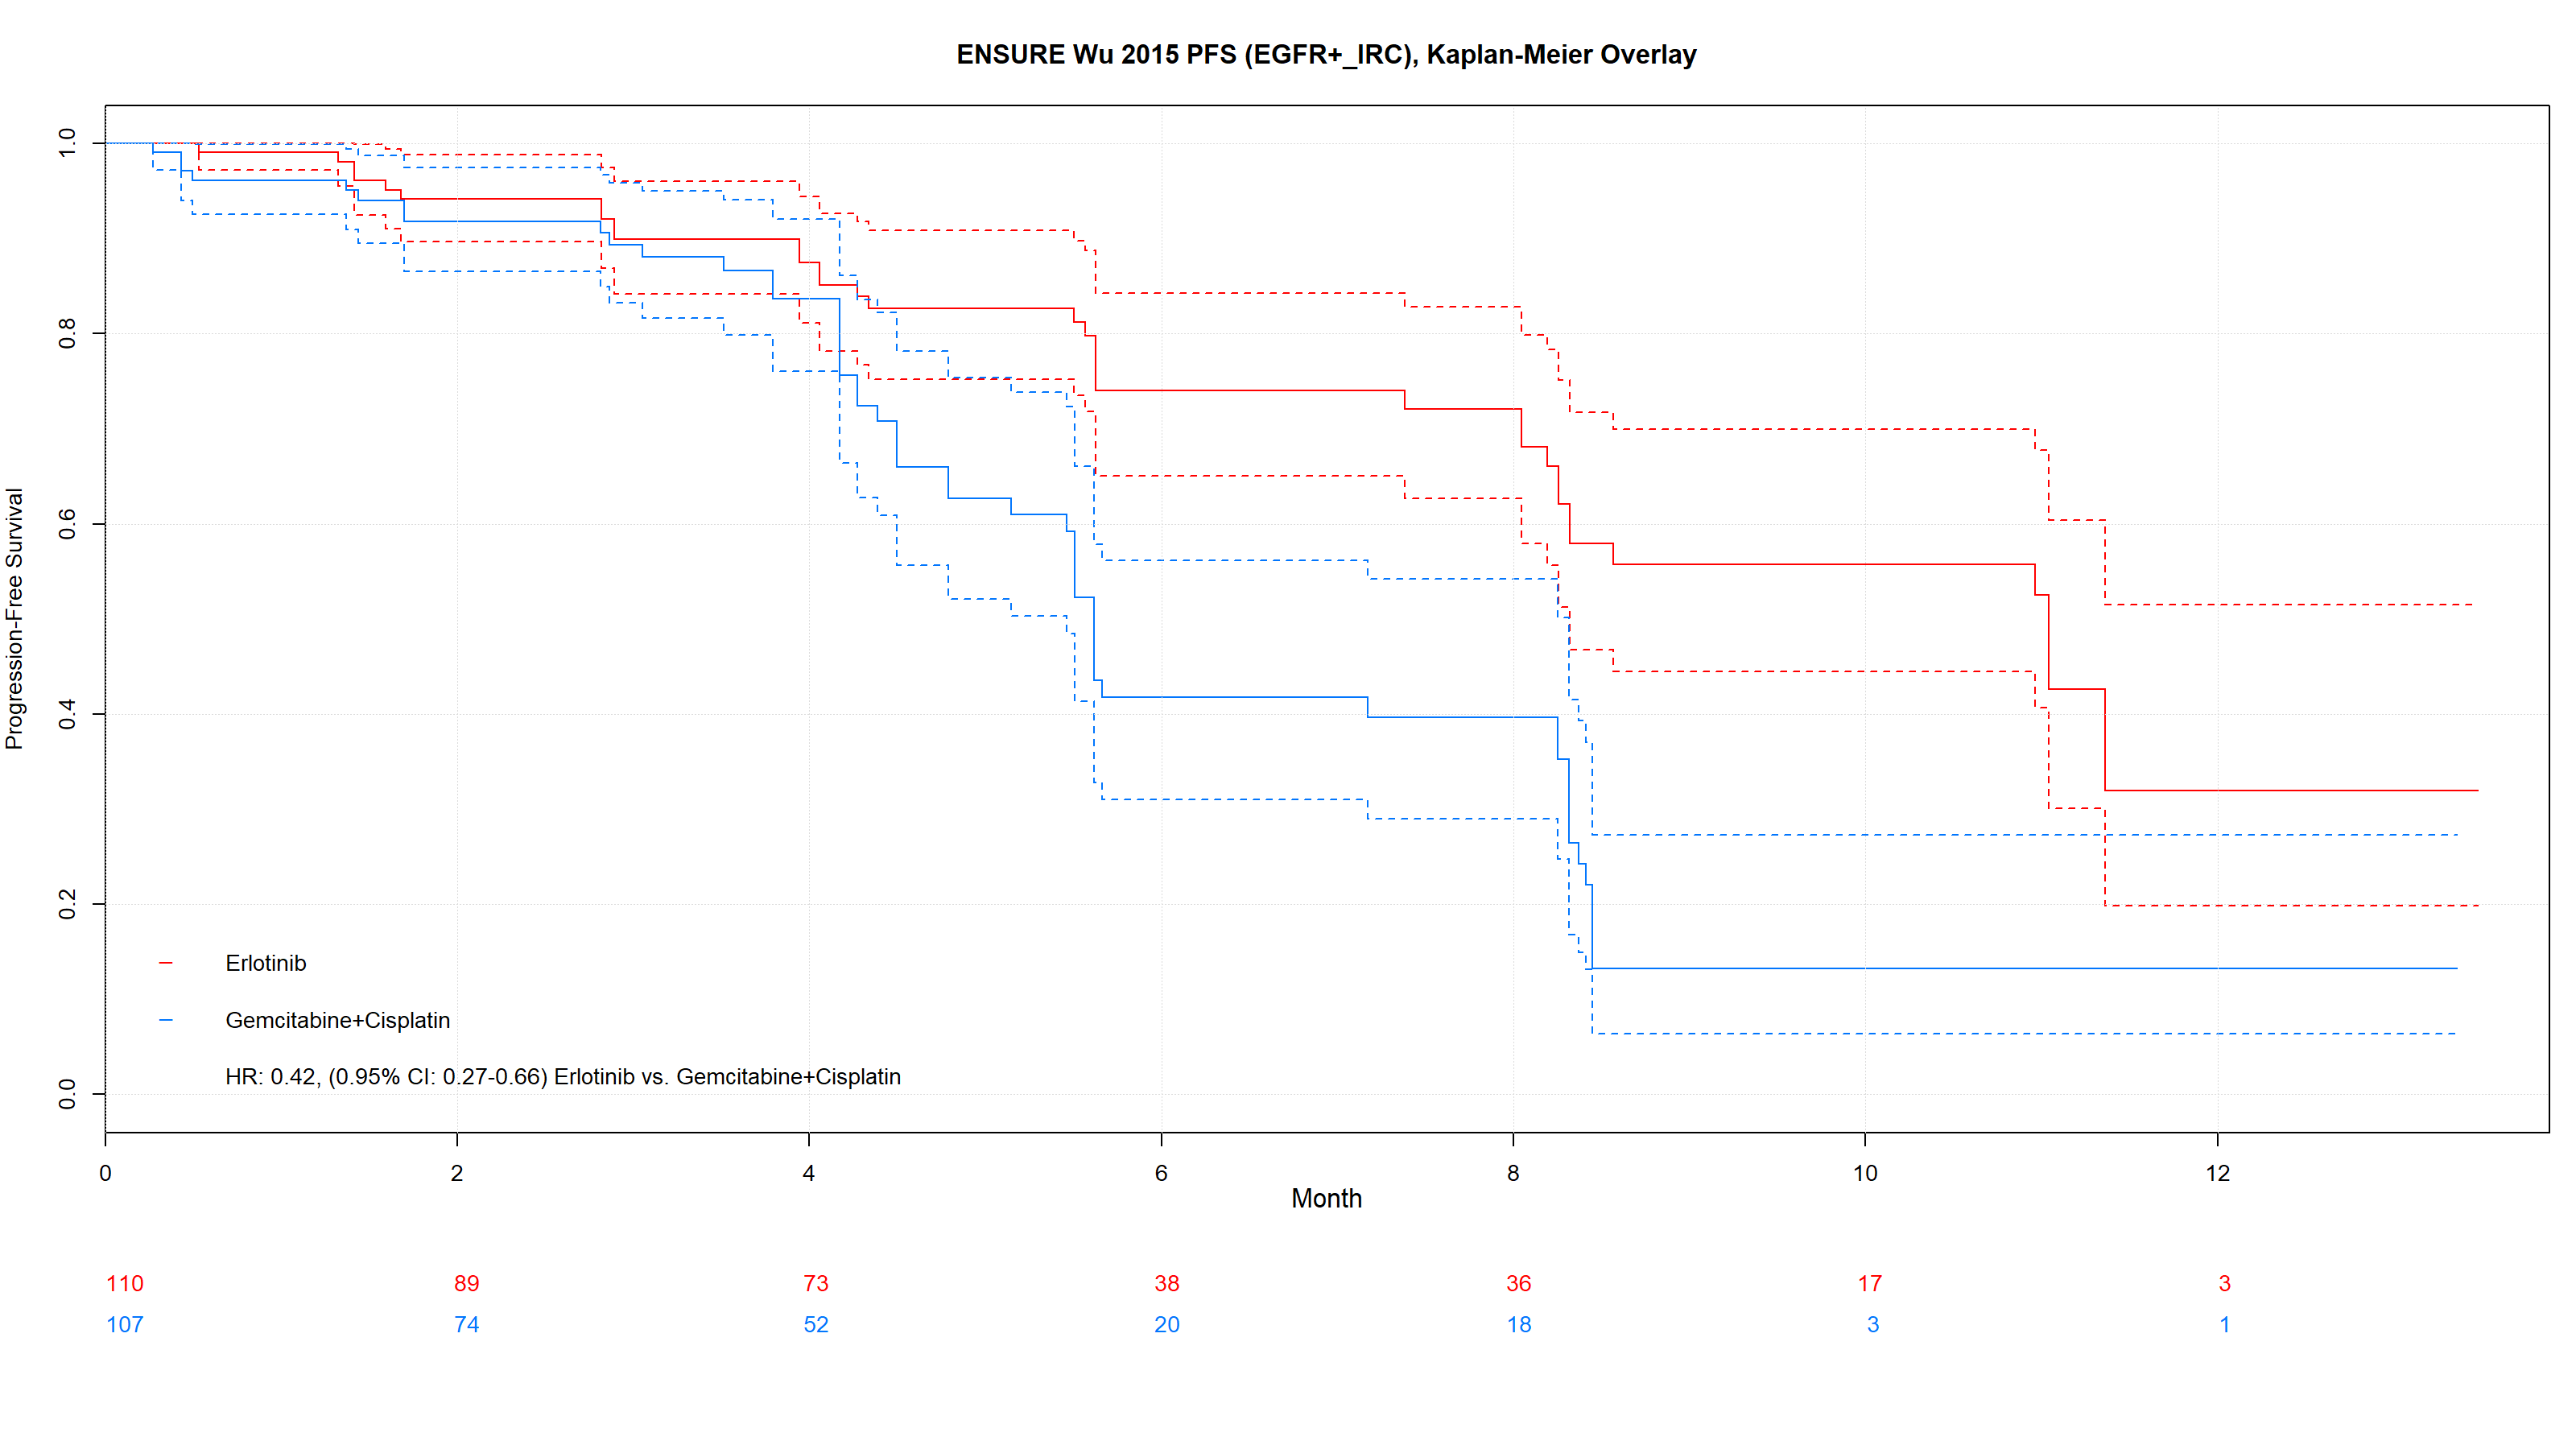
\includegraphics[max size={\textwidth}{\textheight}]{figs/km-plots/ENSURE Wu 2015 PFS (EGFR+_IRC) Kaplan Meier.png}
\end{subfigure}
\begin{subfigure}{\textwidth}
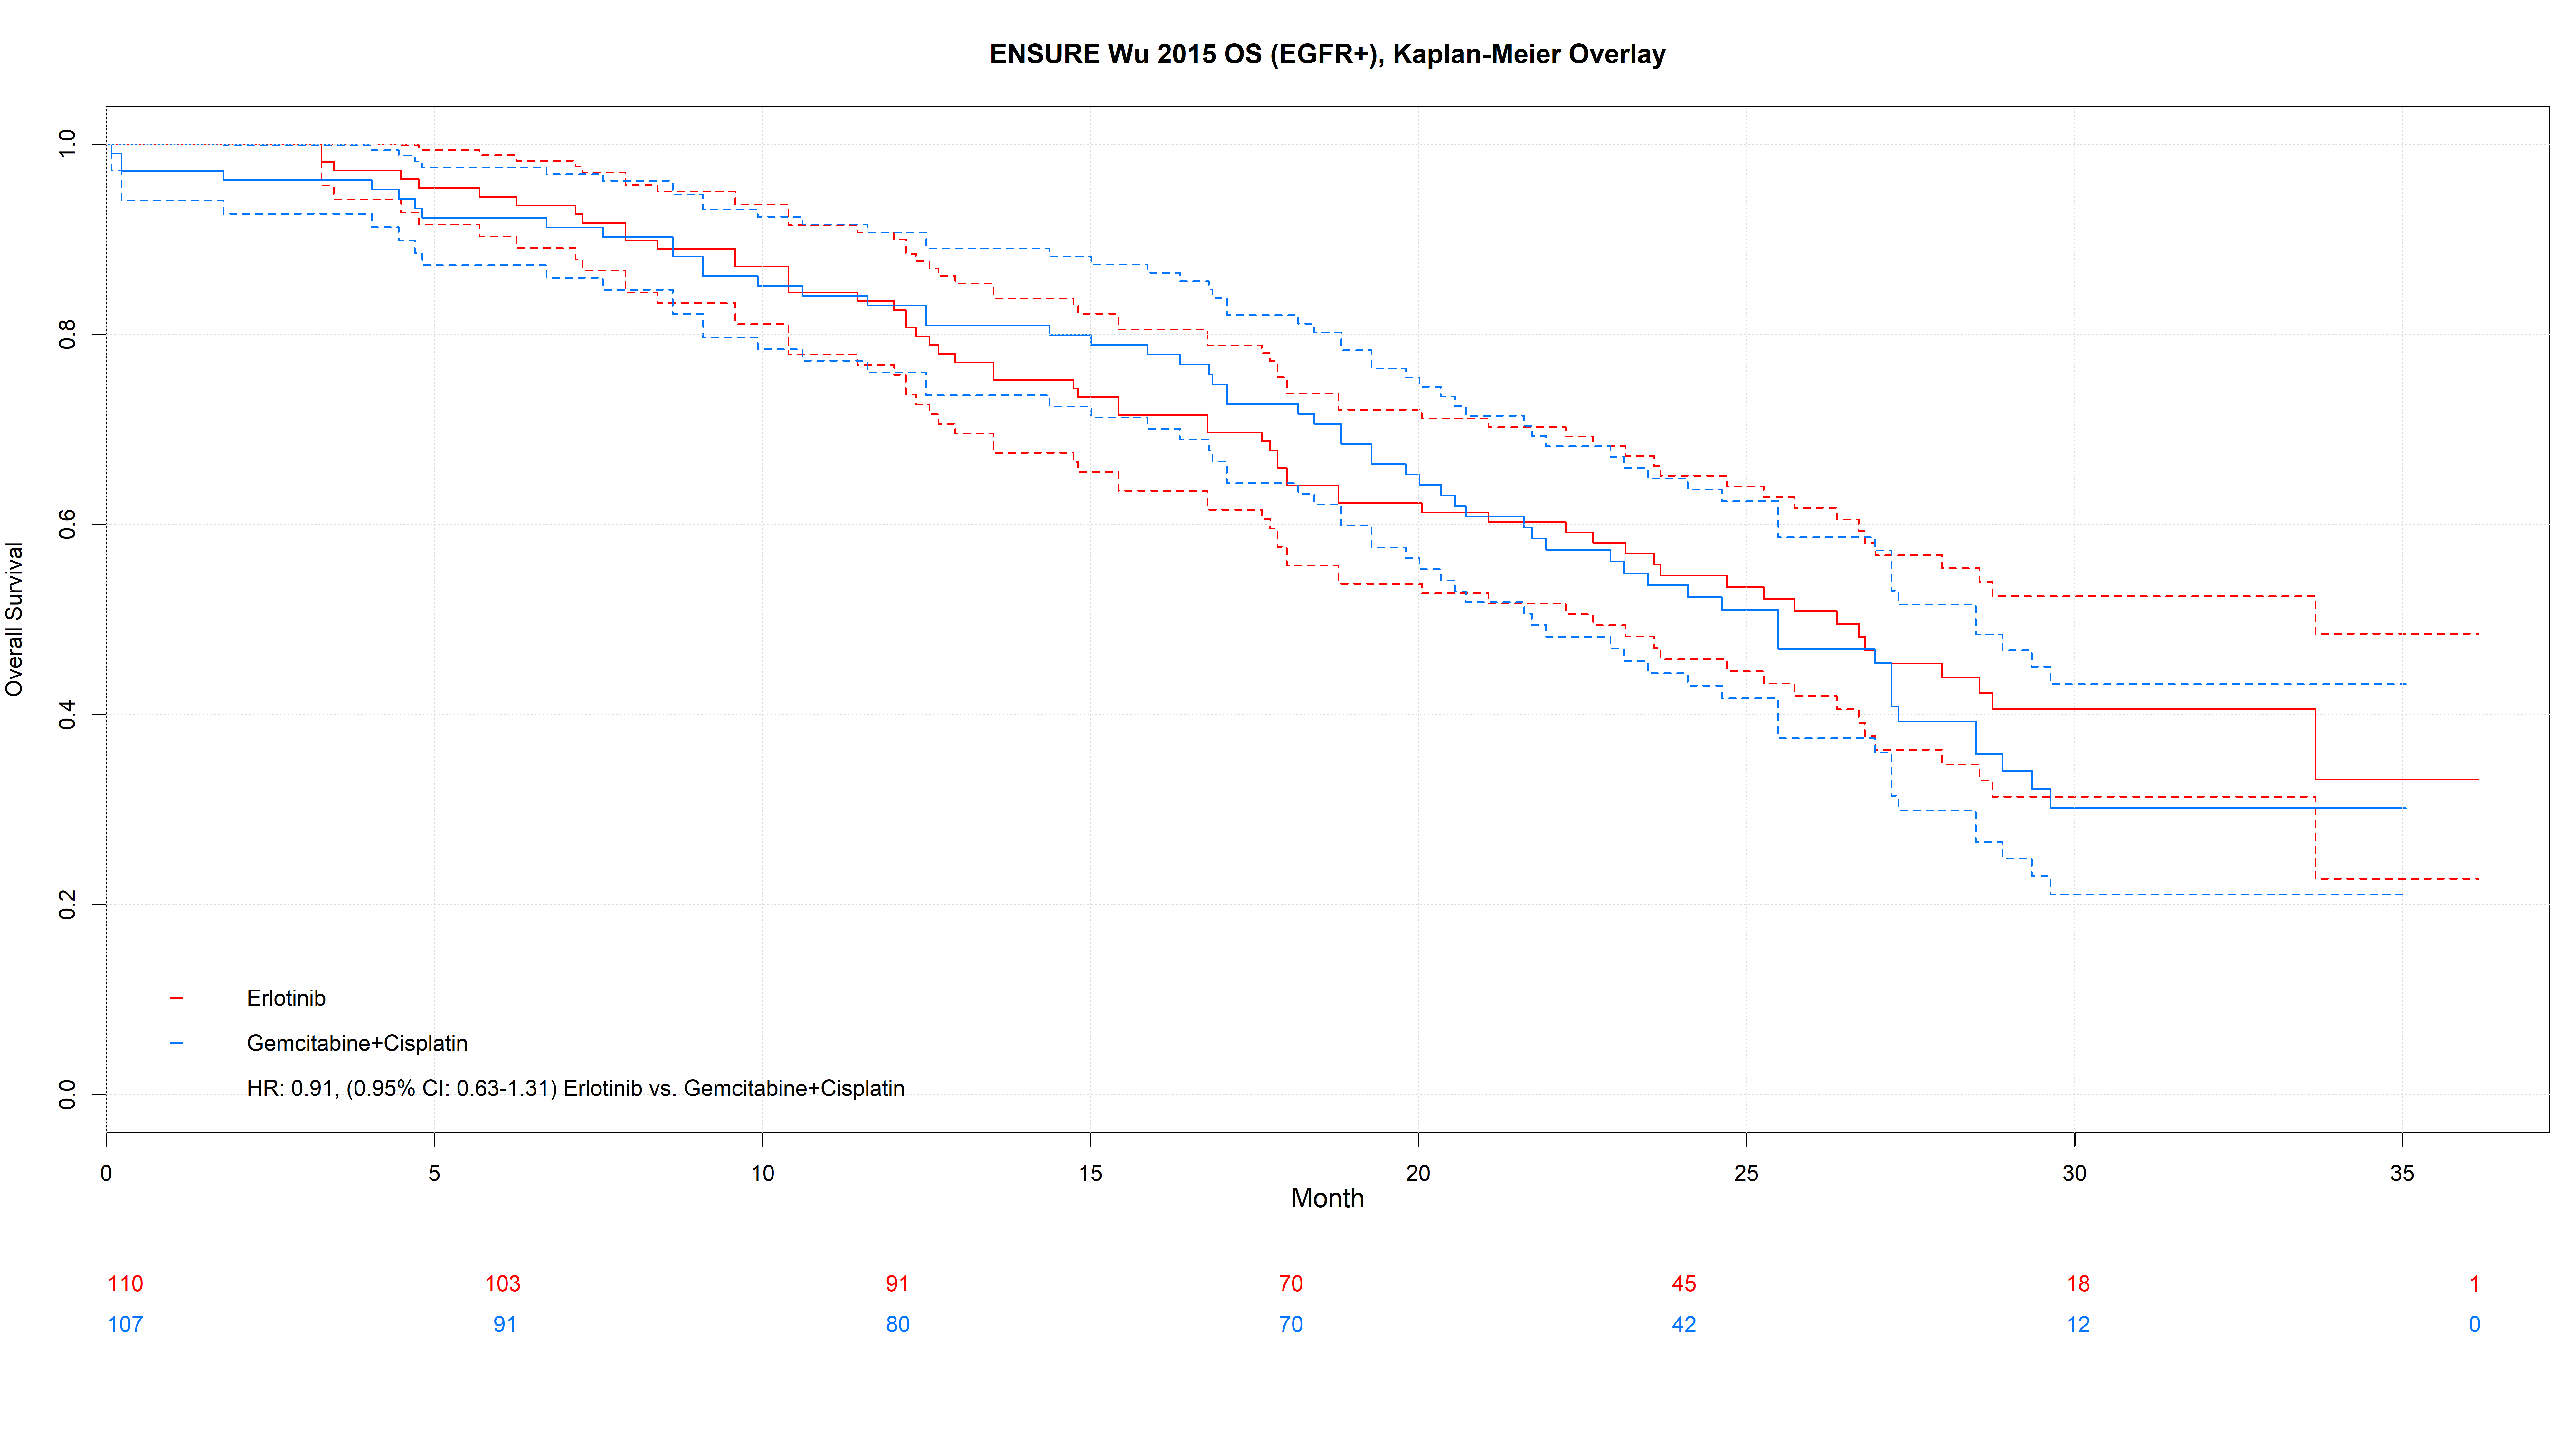
\includegraphics[max size={\textwidth}{\textheight}]{figs/km-plots/ENSURE Wu 2015 OS (EGFR+) Kaplan Meier.png}
\end{subfigure}
\centering
\caption{ENSURE, progression-free survival and overall survival}\label{fig:ENSURE}
\end{figure}


\begin{figure}
\centering
\begin{subfigure}{\textwidth}
\centering
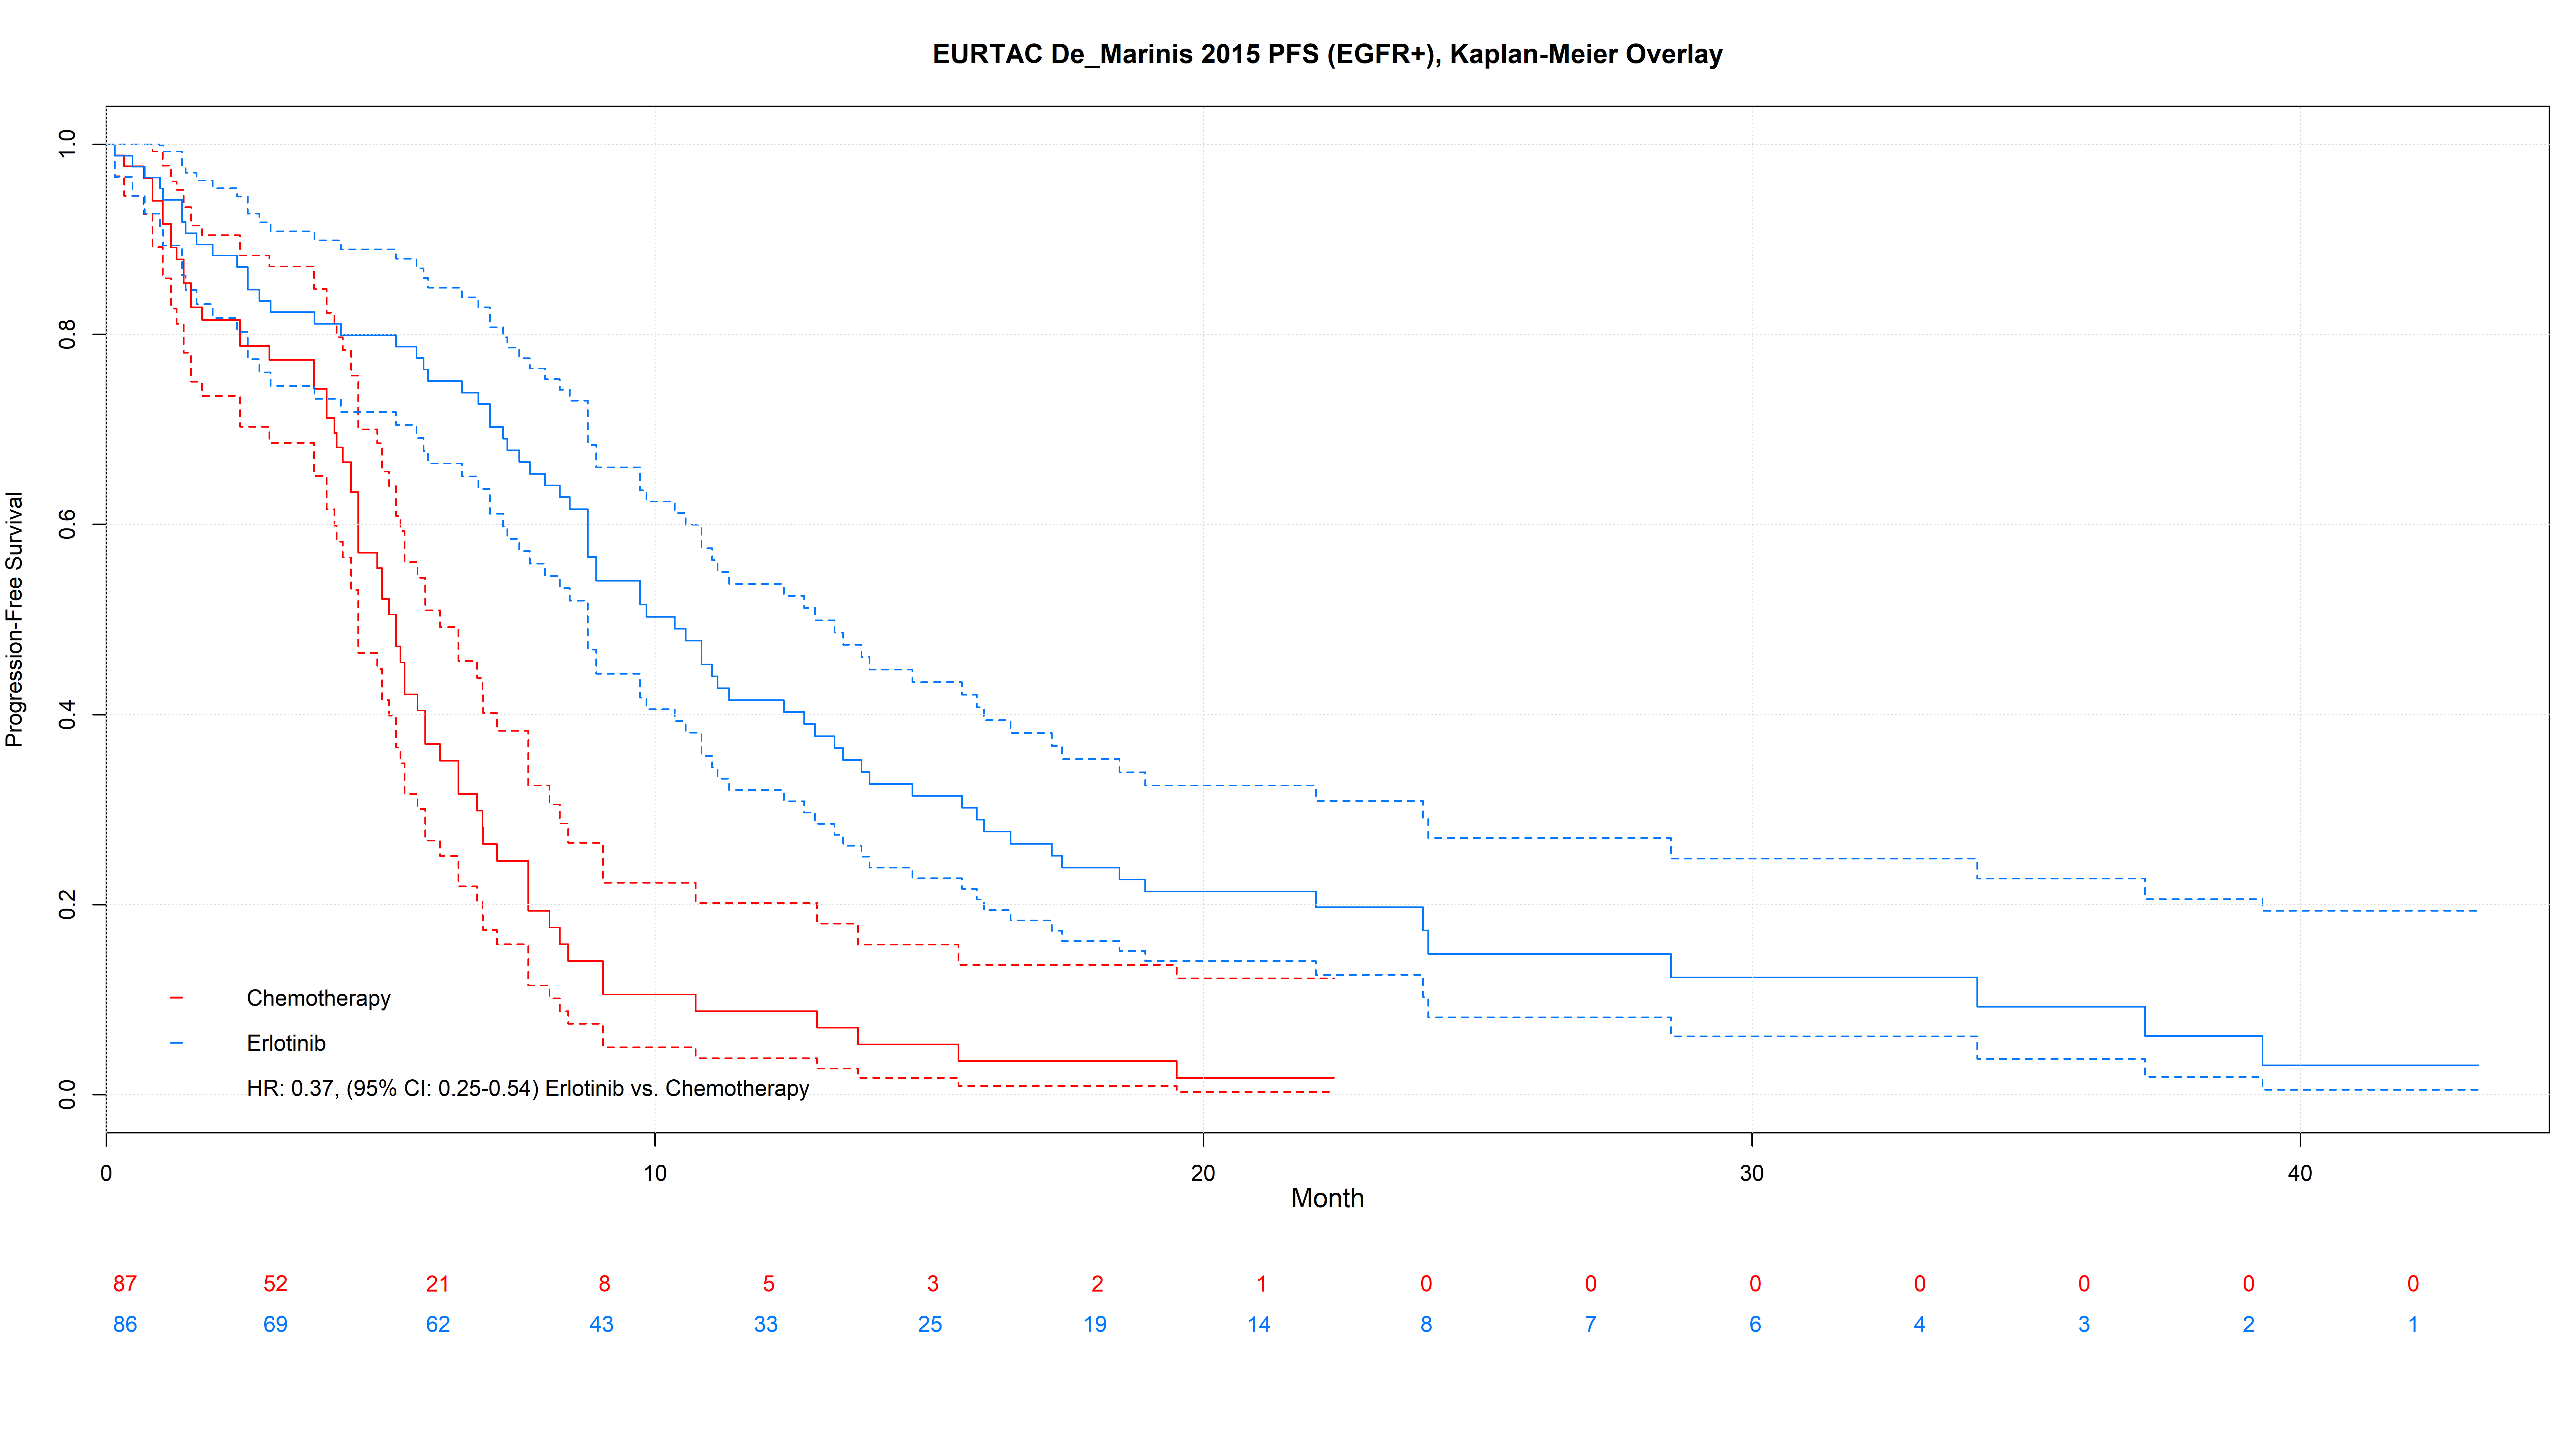
\includegraphics[max size={\textwidth}{\textheight}]{figs/km-plots/EURTAC De_Marinis 2015 PFS (EGFR+) Kaplan Meier.png}
\end{subfigure}
\begin{subfigure}{\textwidth}
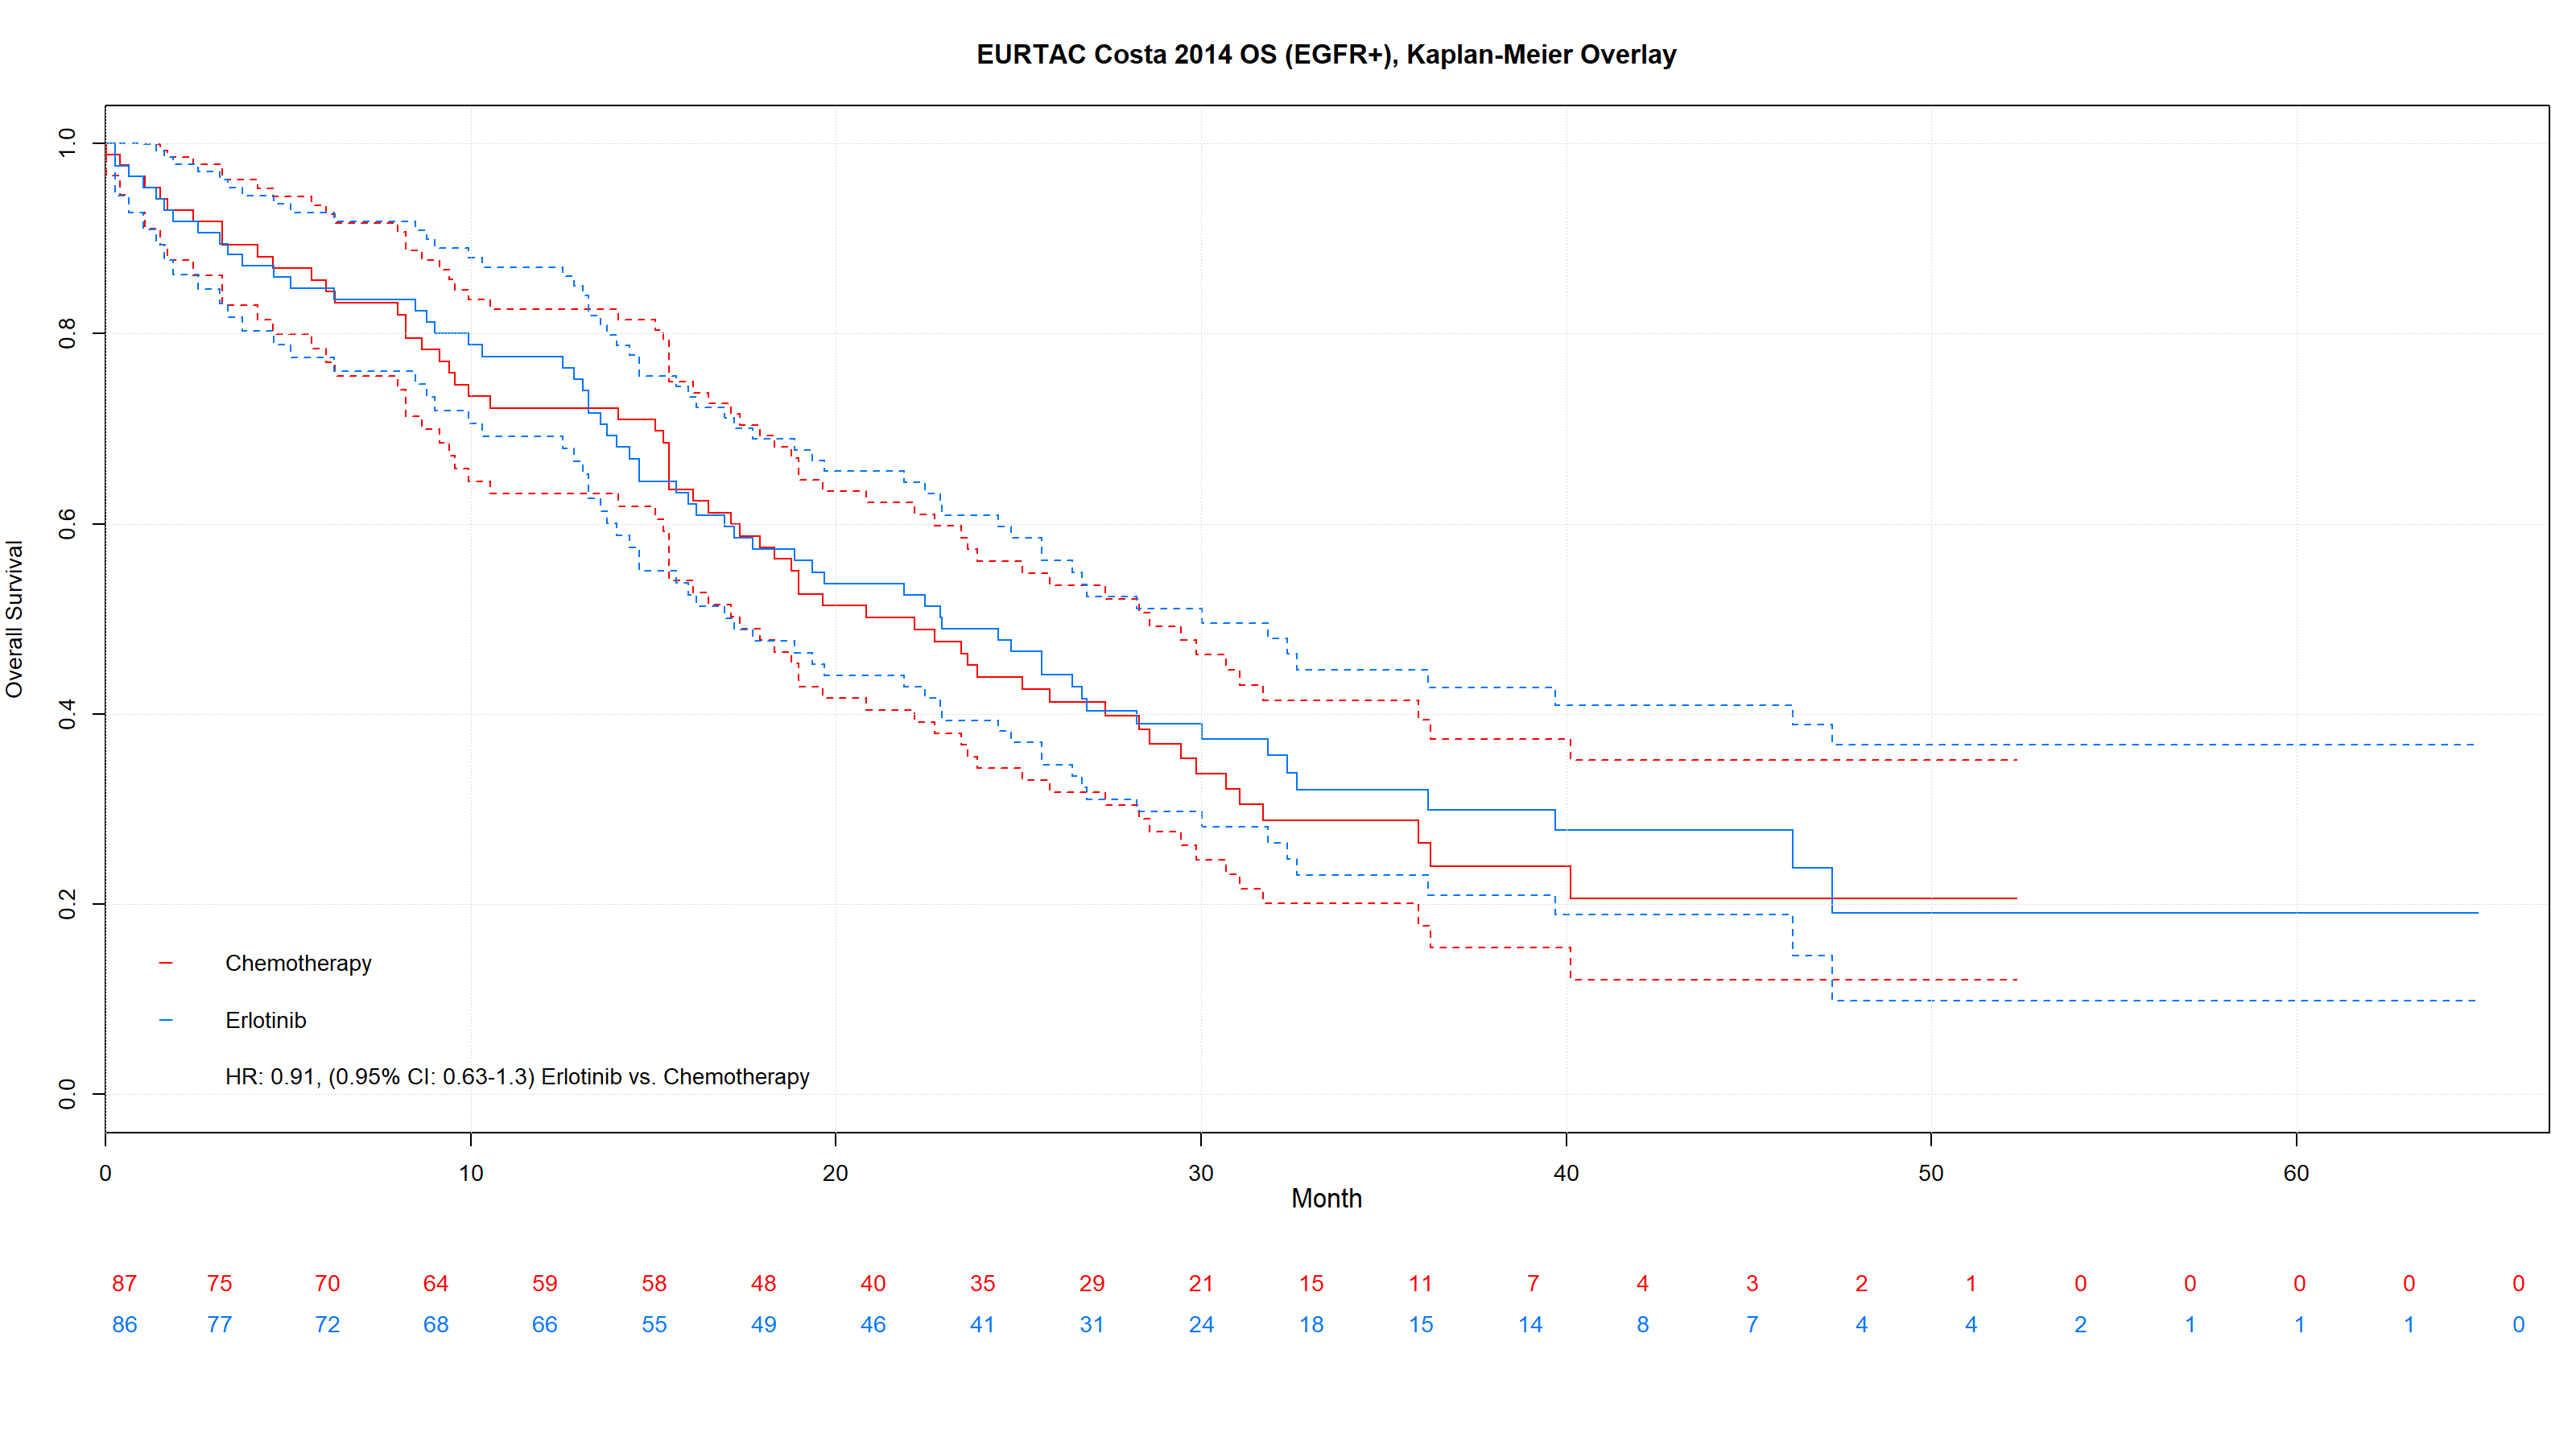
\includegraphics[max size={\textwidth}{\textheight}]{figs/km-plots/EURTAC Costa 2014 OS (EGFR+) Kaplan Meier.png}
\end{subfigure}
\centering
\caption{EURTAC, progression-free survival and overall survival}\label{fig:EURTAC}
\end{figure}


\begin{figure}
\centering
\begin{subfigure}{\textwidth}
\centering
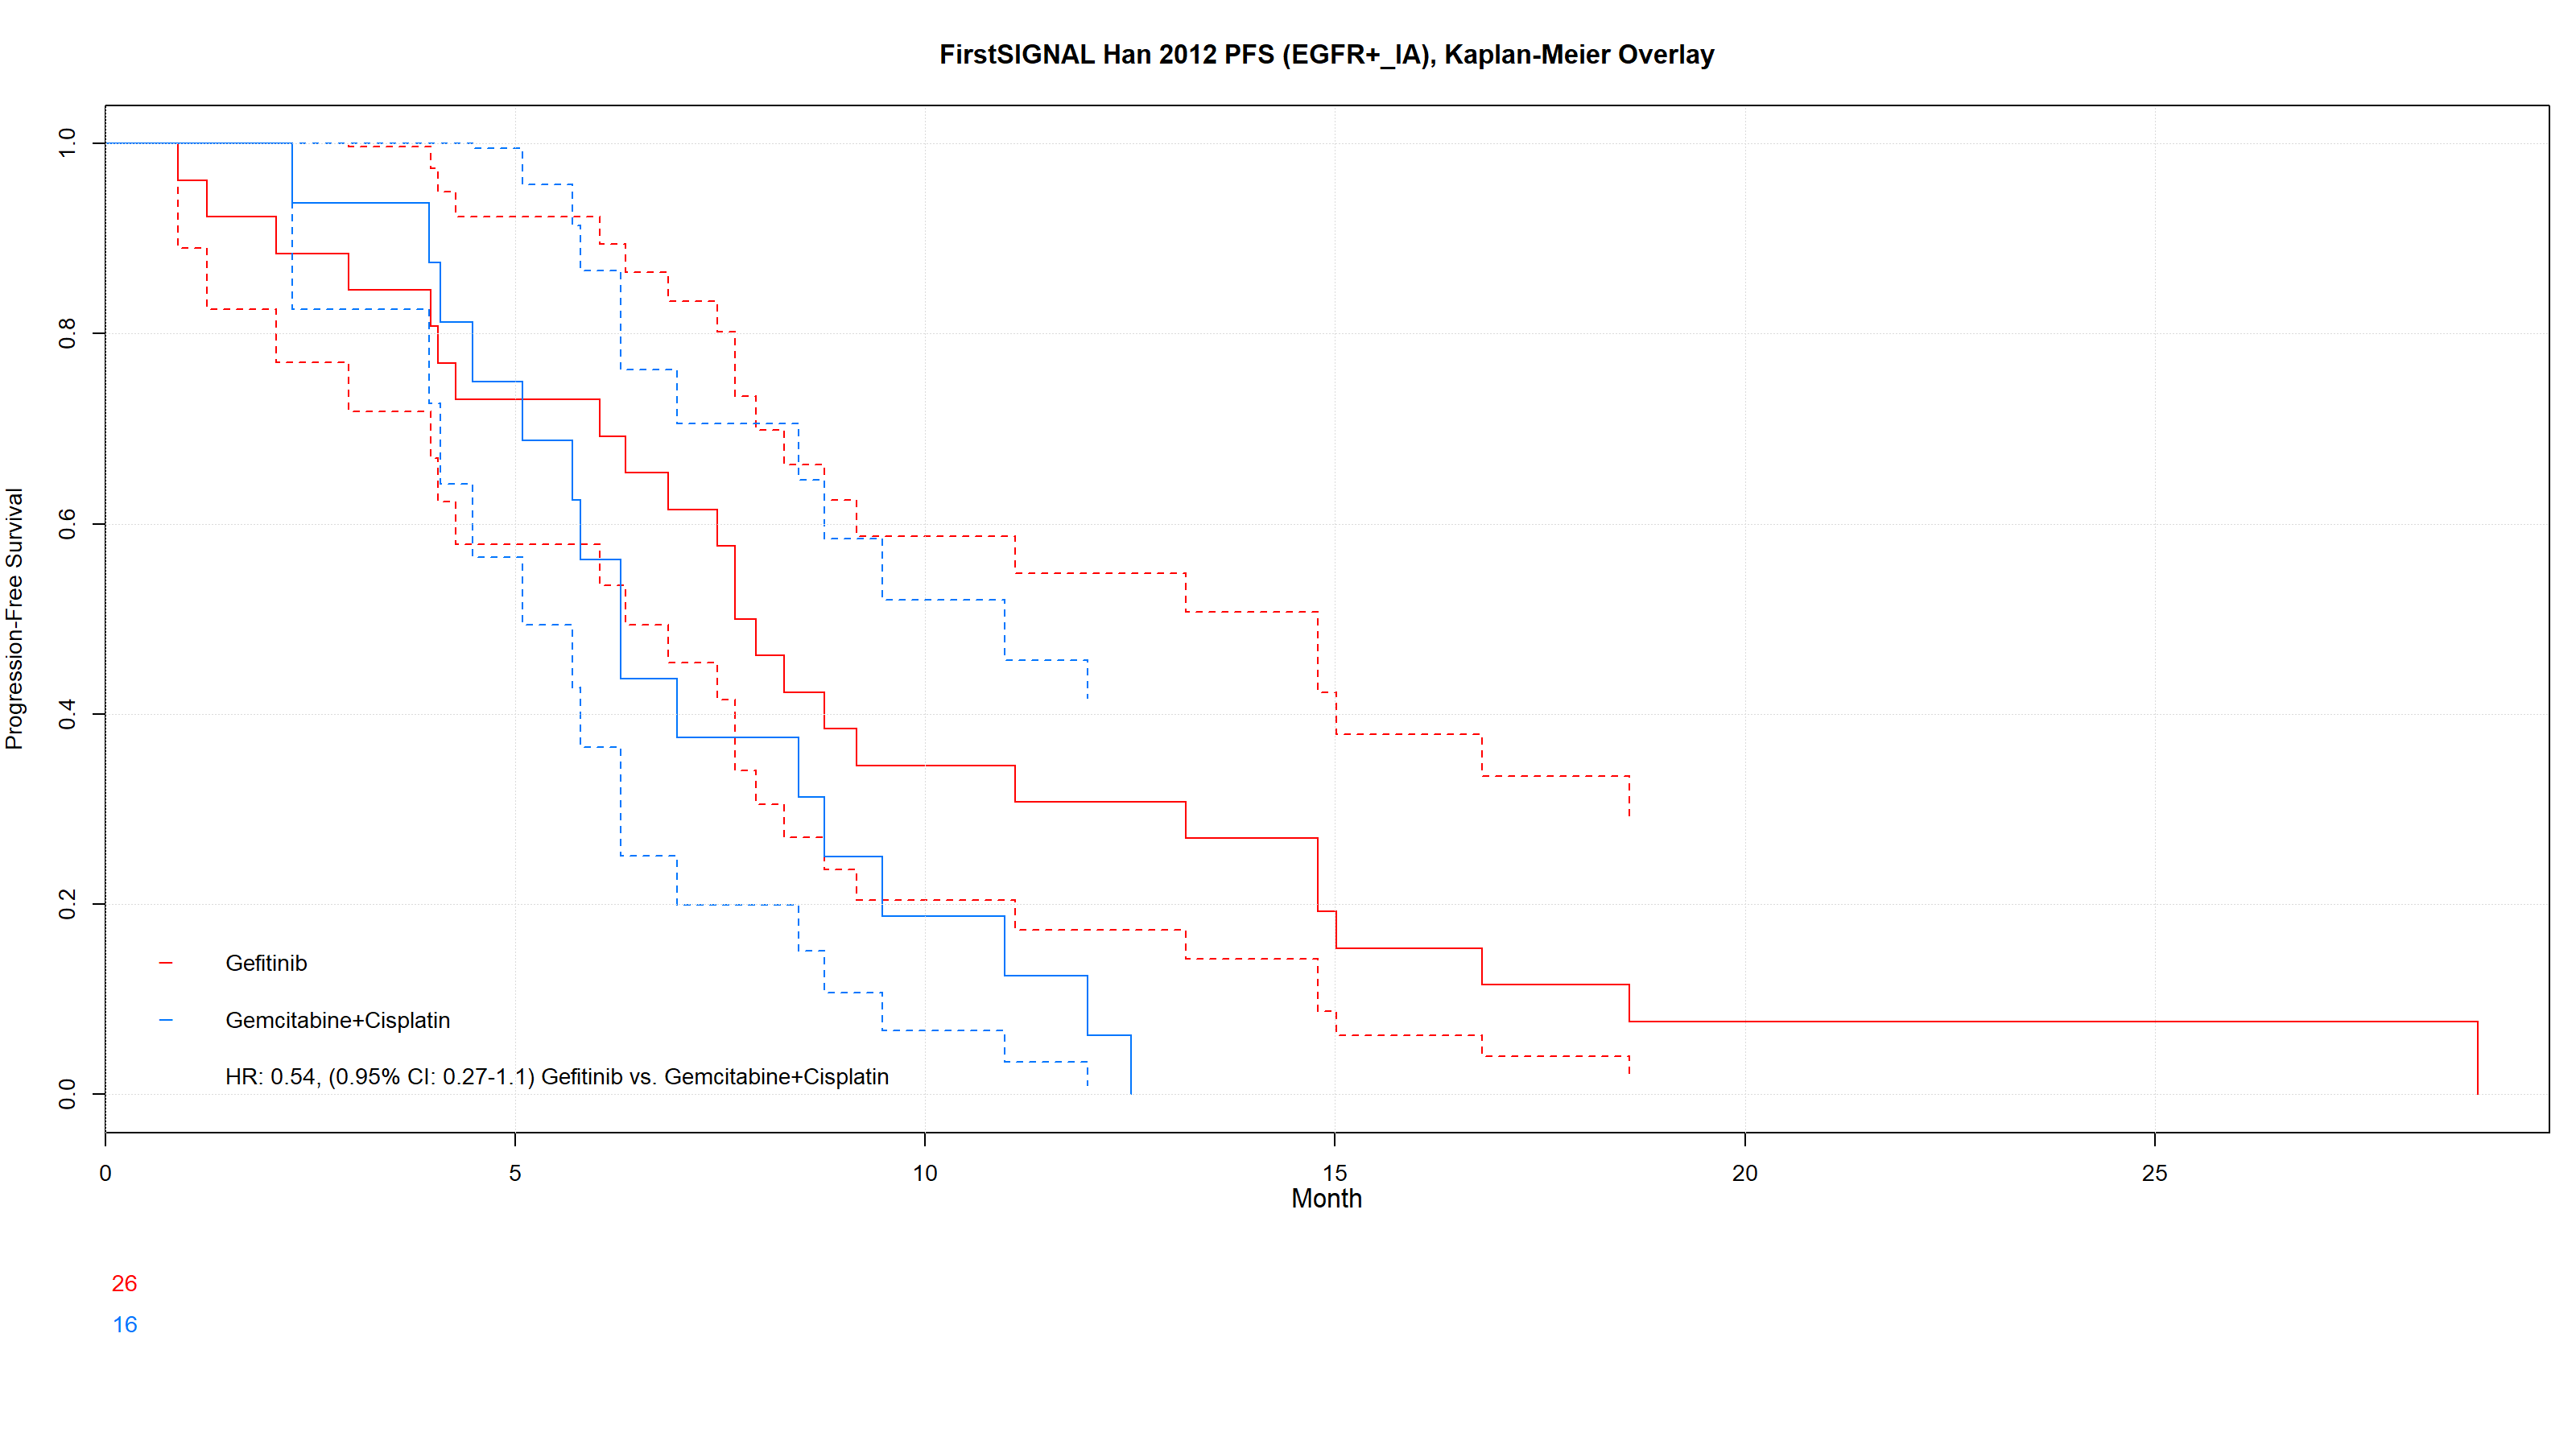
\includegraphics[max size={\textwidth}{\textheight}]{figs/km-plots/FirstSIGNAL Han 2012 PFS (EGFR+_IA) Kaplan Meier.png}
\end{subfigure}
\begin{subfigure}{\textwidth}
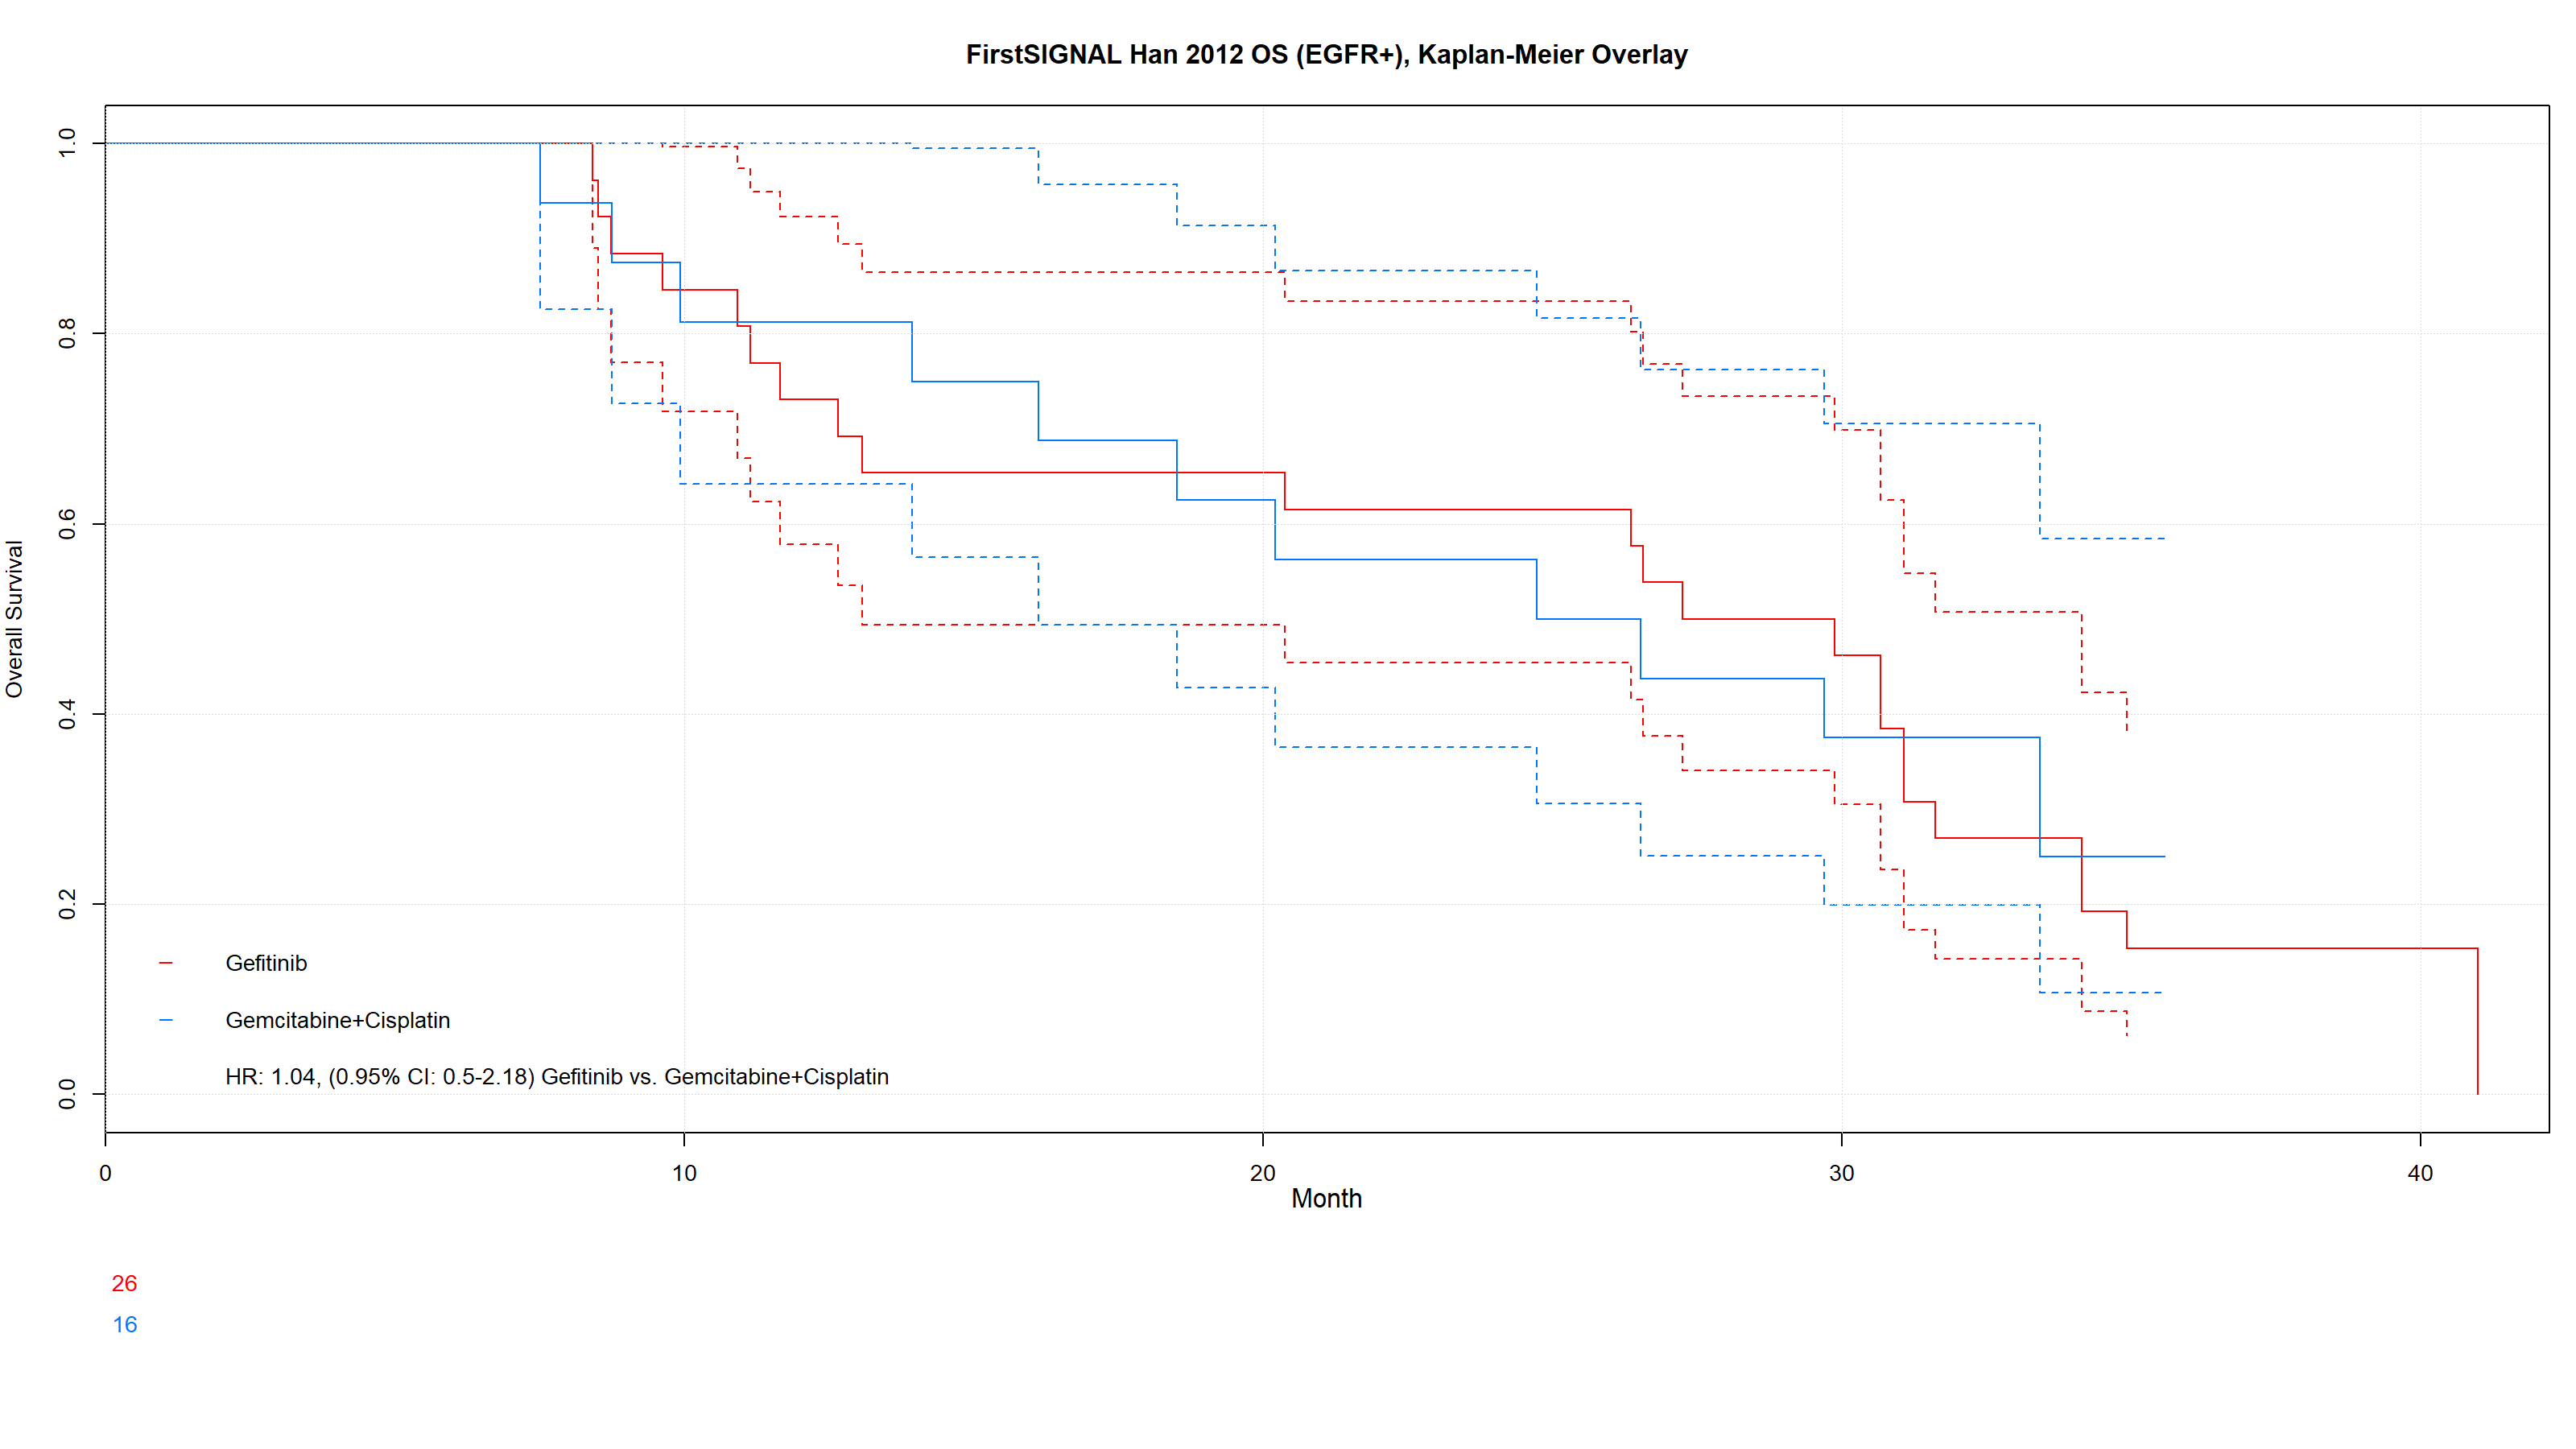
\includegraphics[max size={\textwidth}{\textheight}]{figs/km-plots/FirstSIGNAL Han 2012 OS (EGFR+) Kaplan Meier.png}
\end{subfigure}
\centering
\caption{FirstSIGNAL, progression-free survival and overall survival}\label{fig:firstSIGNAL}
\end{figure}


\begin{figure}
\centering
\begin{subfigure}{\textwidth}
\centering
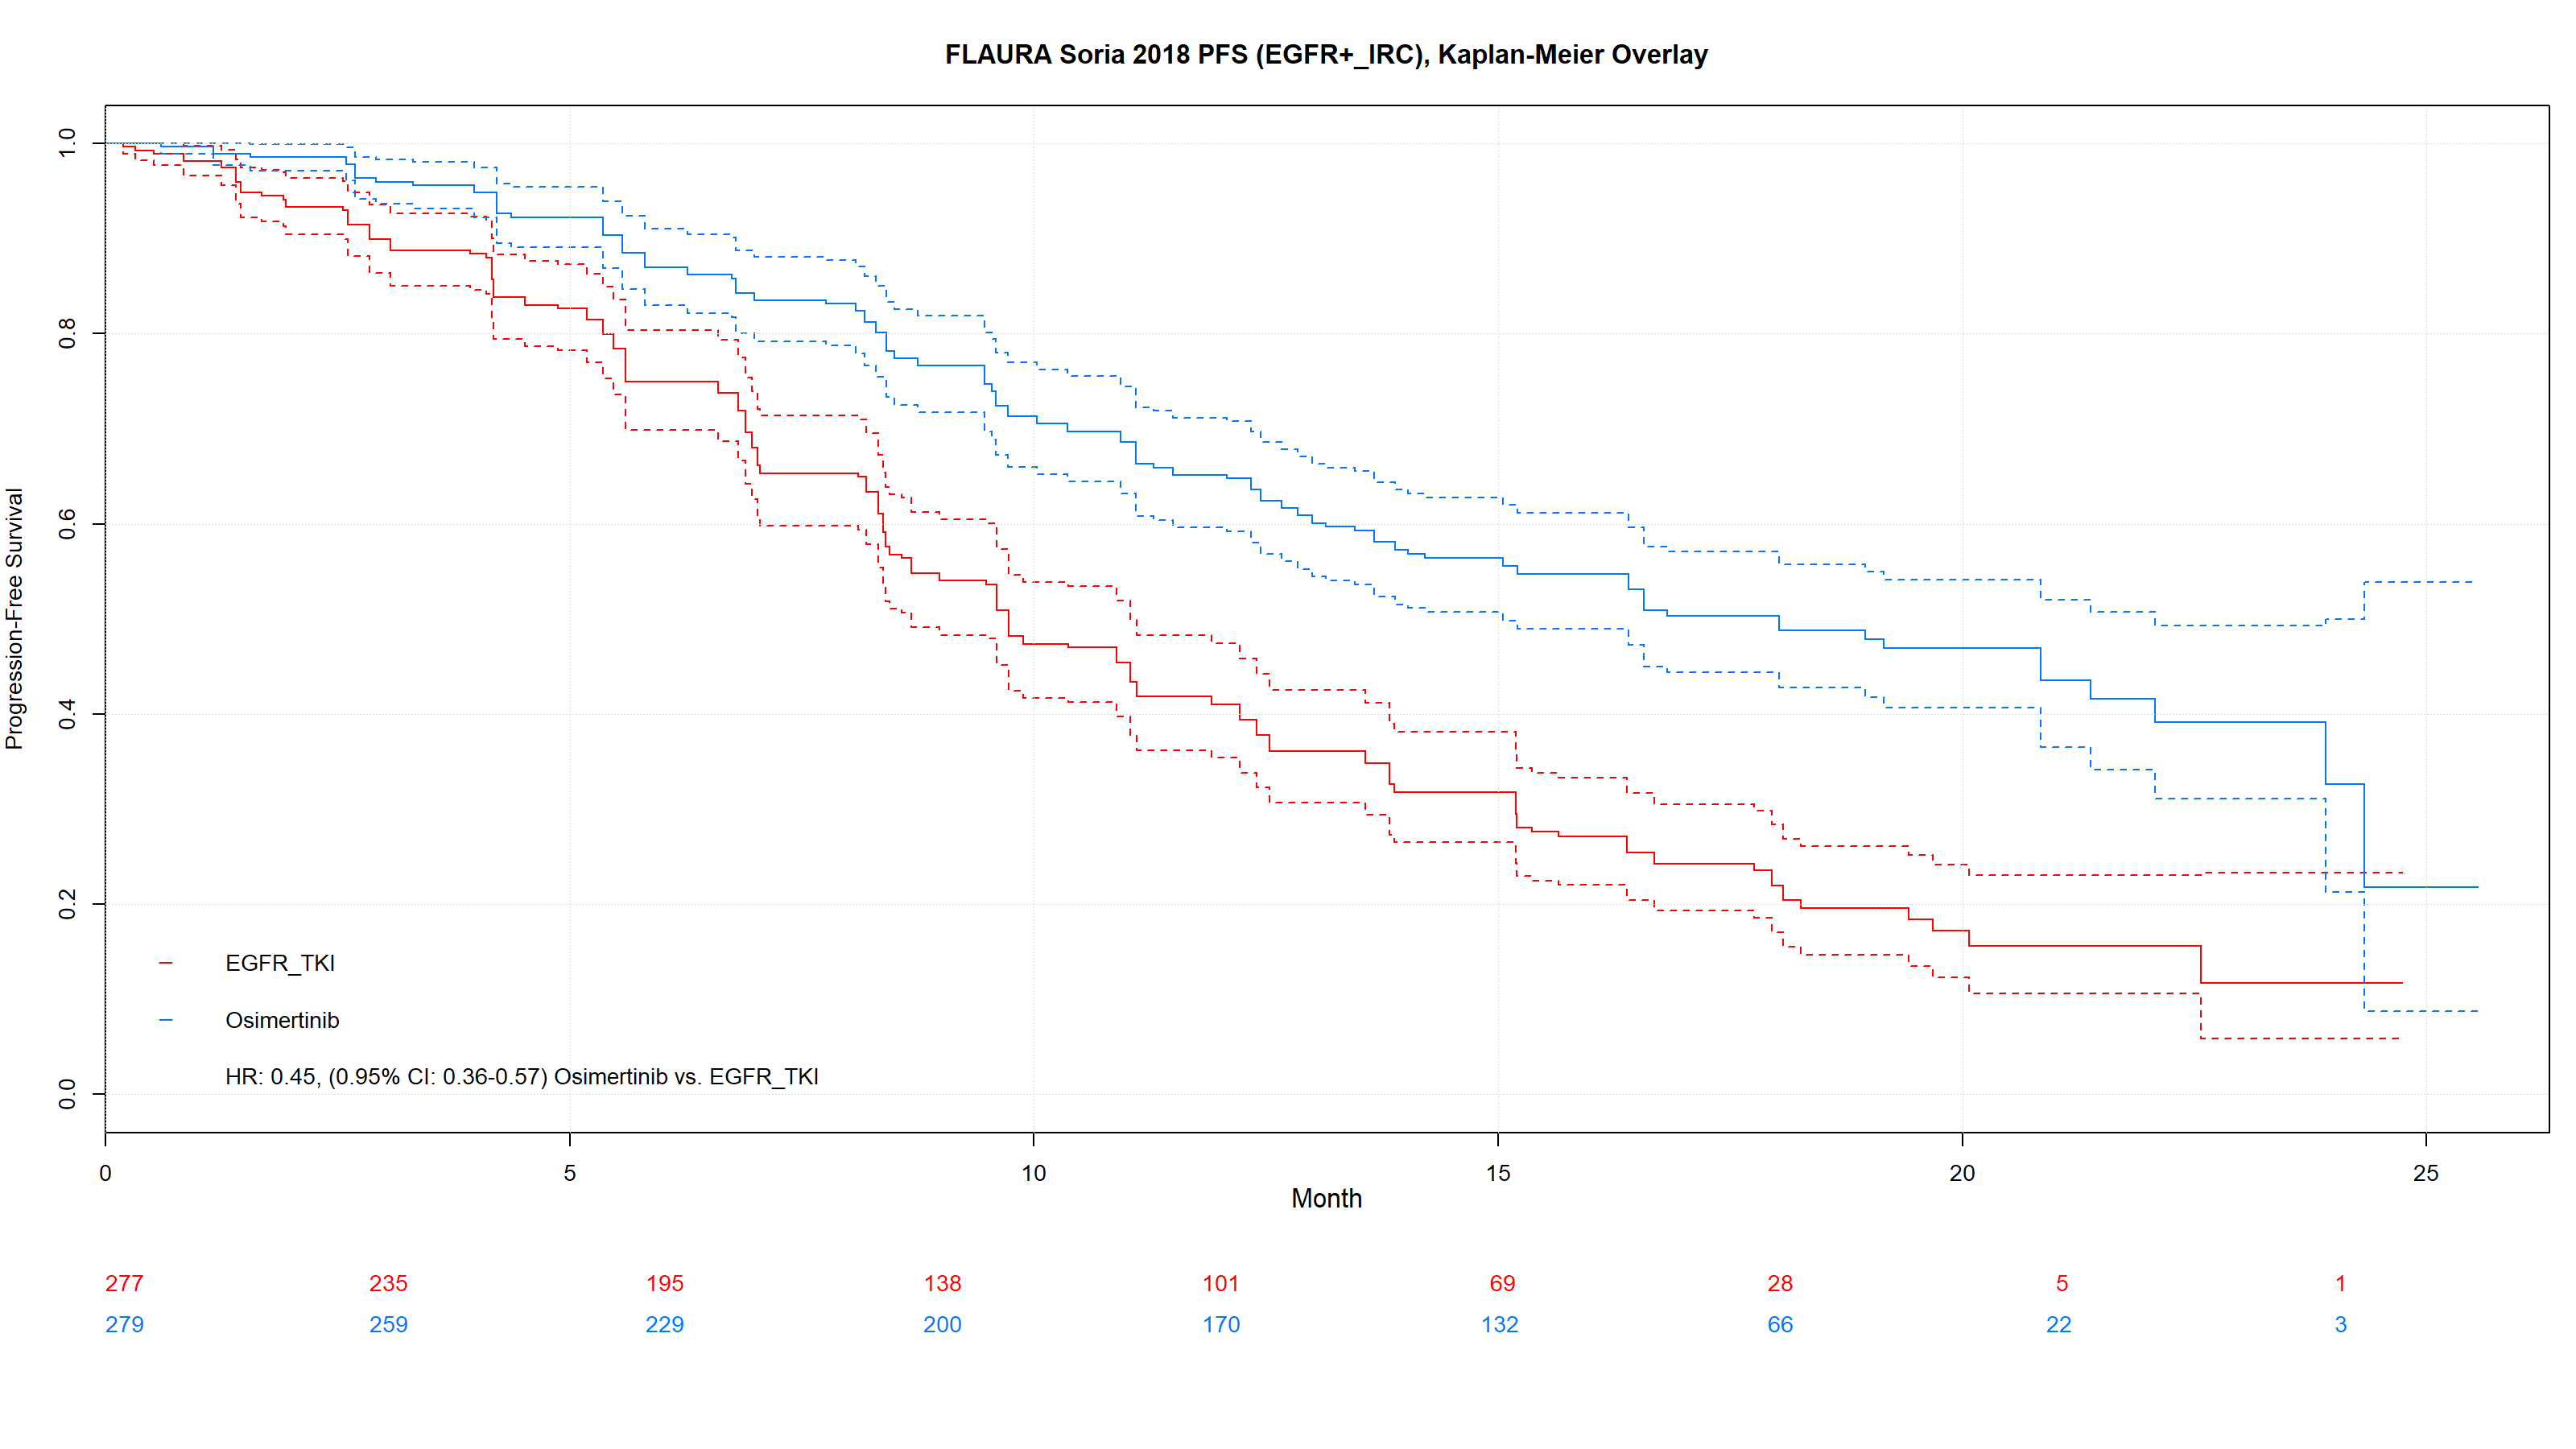
\includegraphics[max size={\textwidth}{\textheight}]{figs/km-plots/FLAURA Soria 2018 PFS (EGFR+_IRC) Kaplan Meier.png}
\end{subfigure}
\begin{subfigure}{\textwidth}
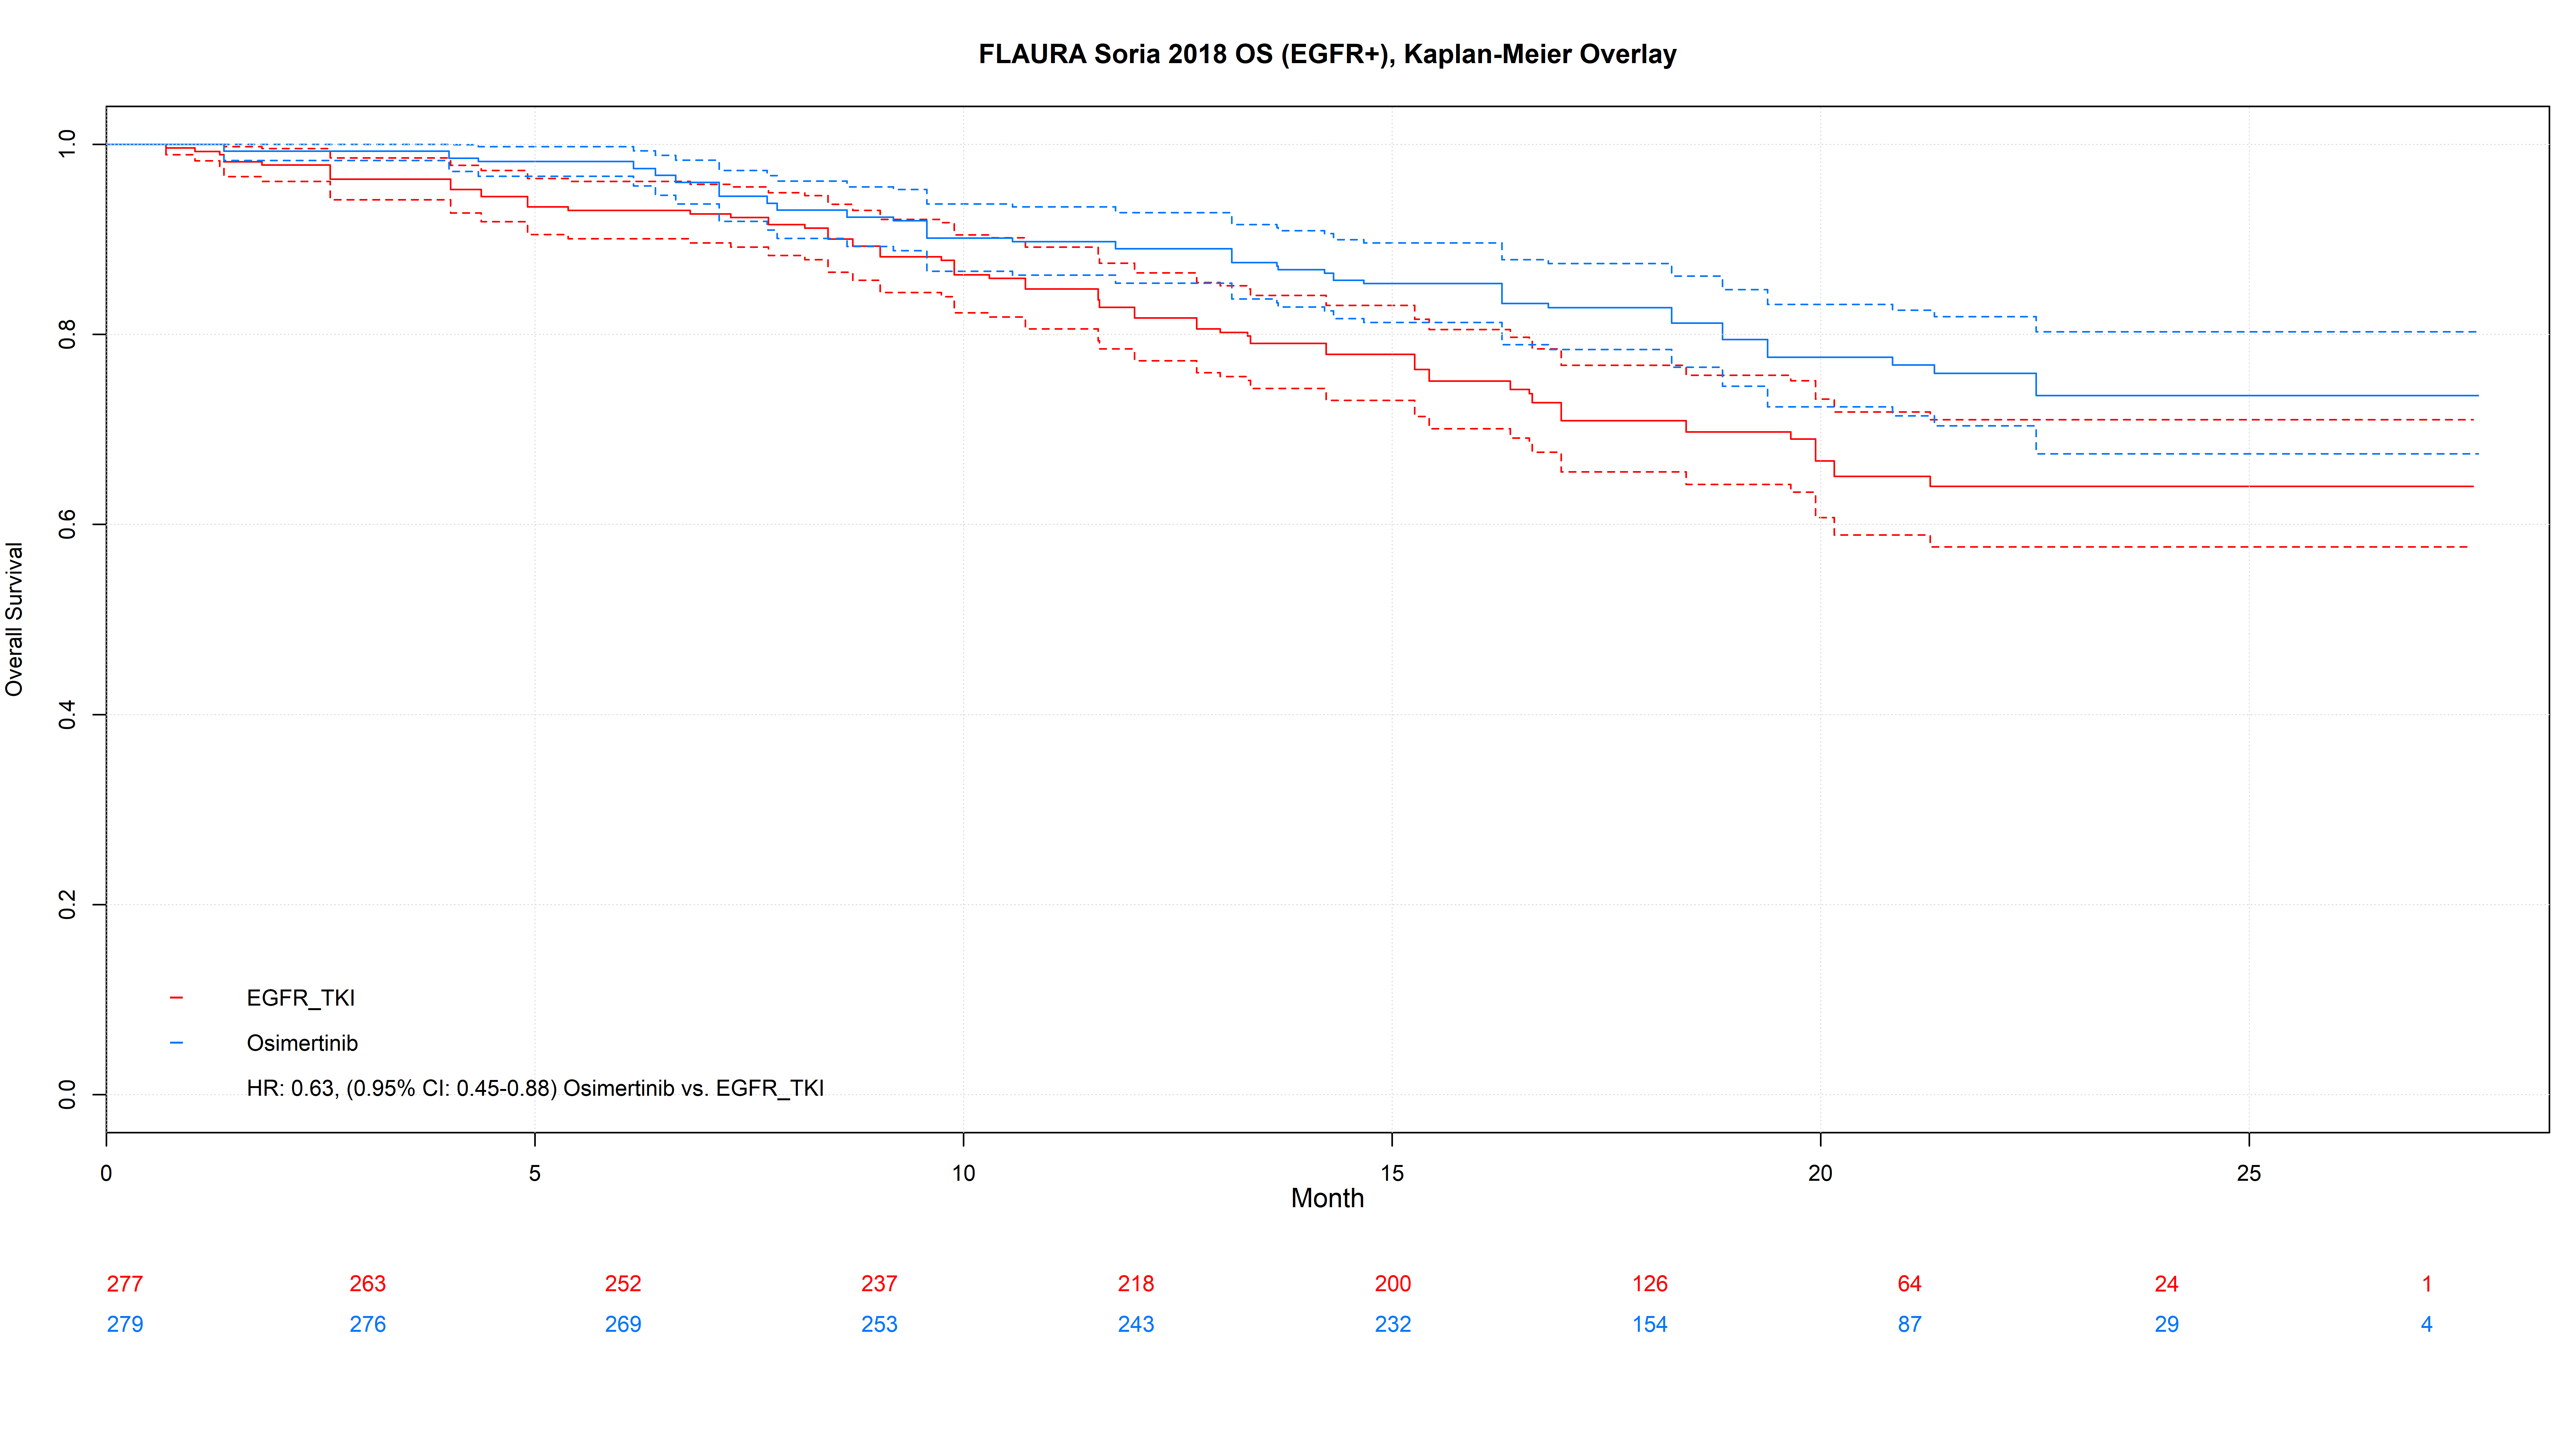
\includegraphics[max size={\textwidth}{\textheight}]{figs/km-plots/FLAURA Soria 2018 OS (EGFR+) Kaplan Meier.png}
\end{subfigure}
\centering
\caption{FLAURA, progression-free survival and overall survival}\label{fig:FLAURA}
\end{figure}


\begin{figure}
\centering
\begin{subfigure}{\textwidth}
\centering
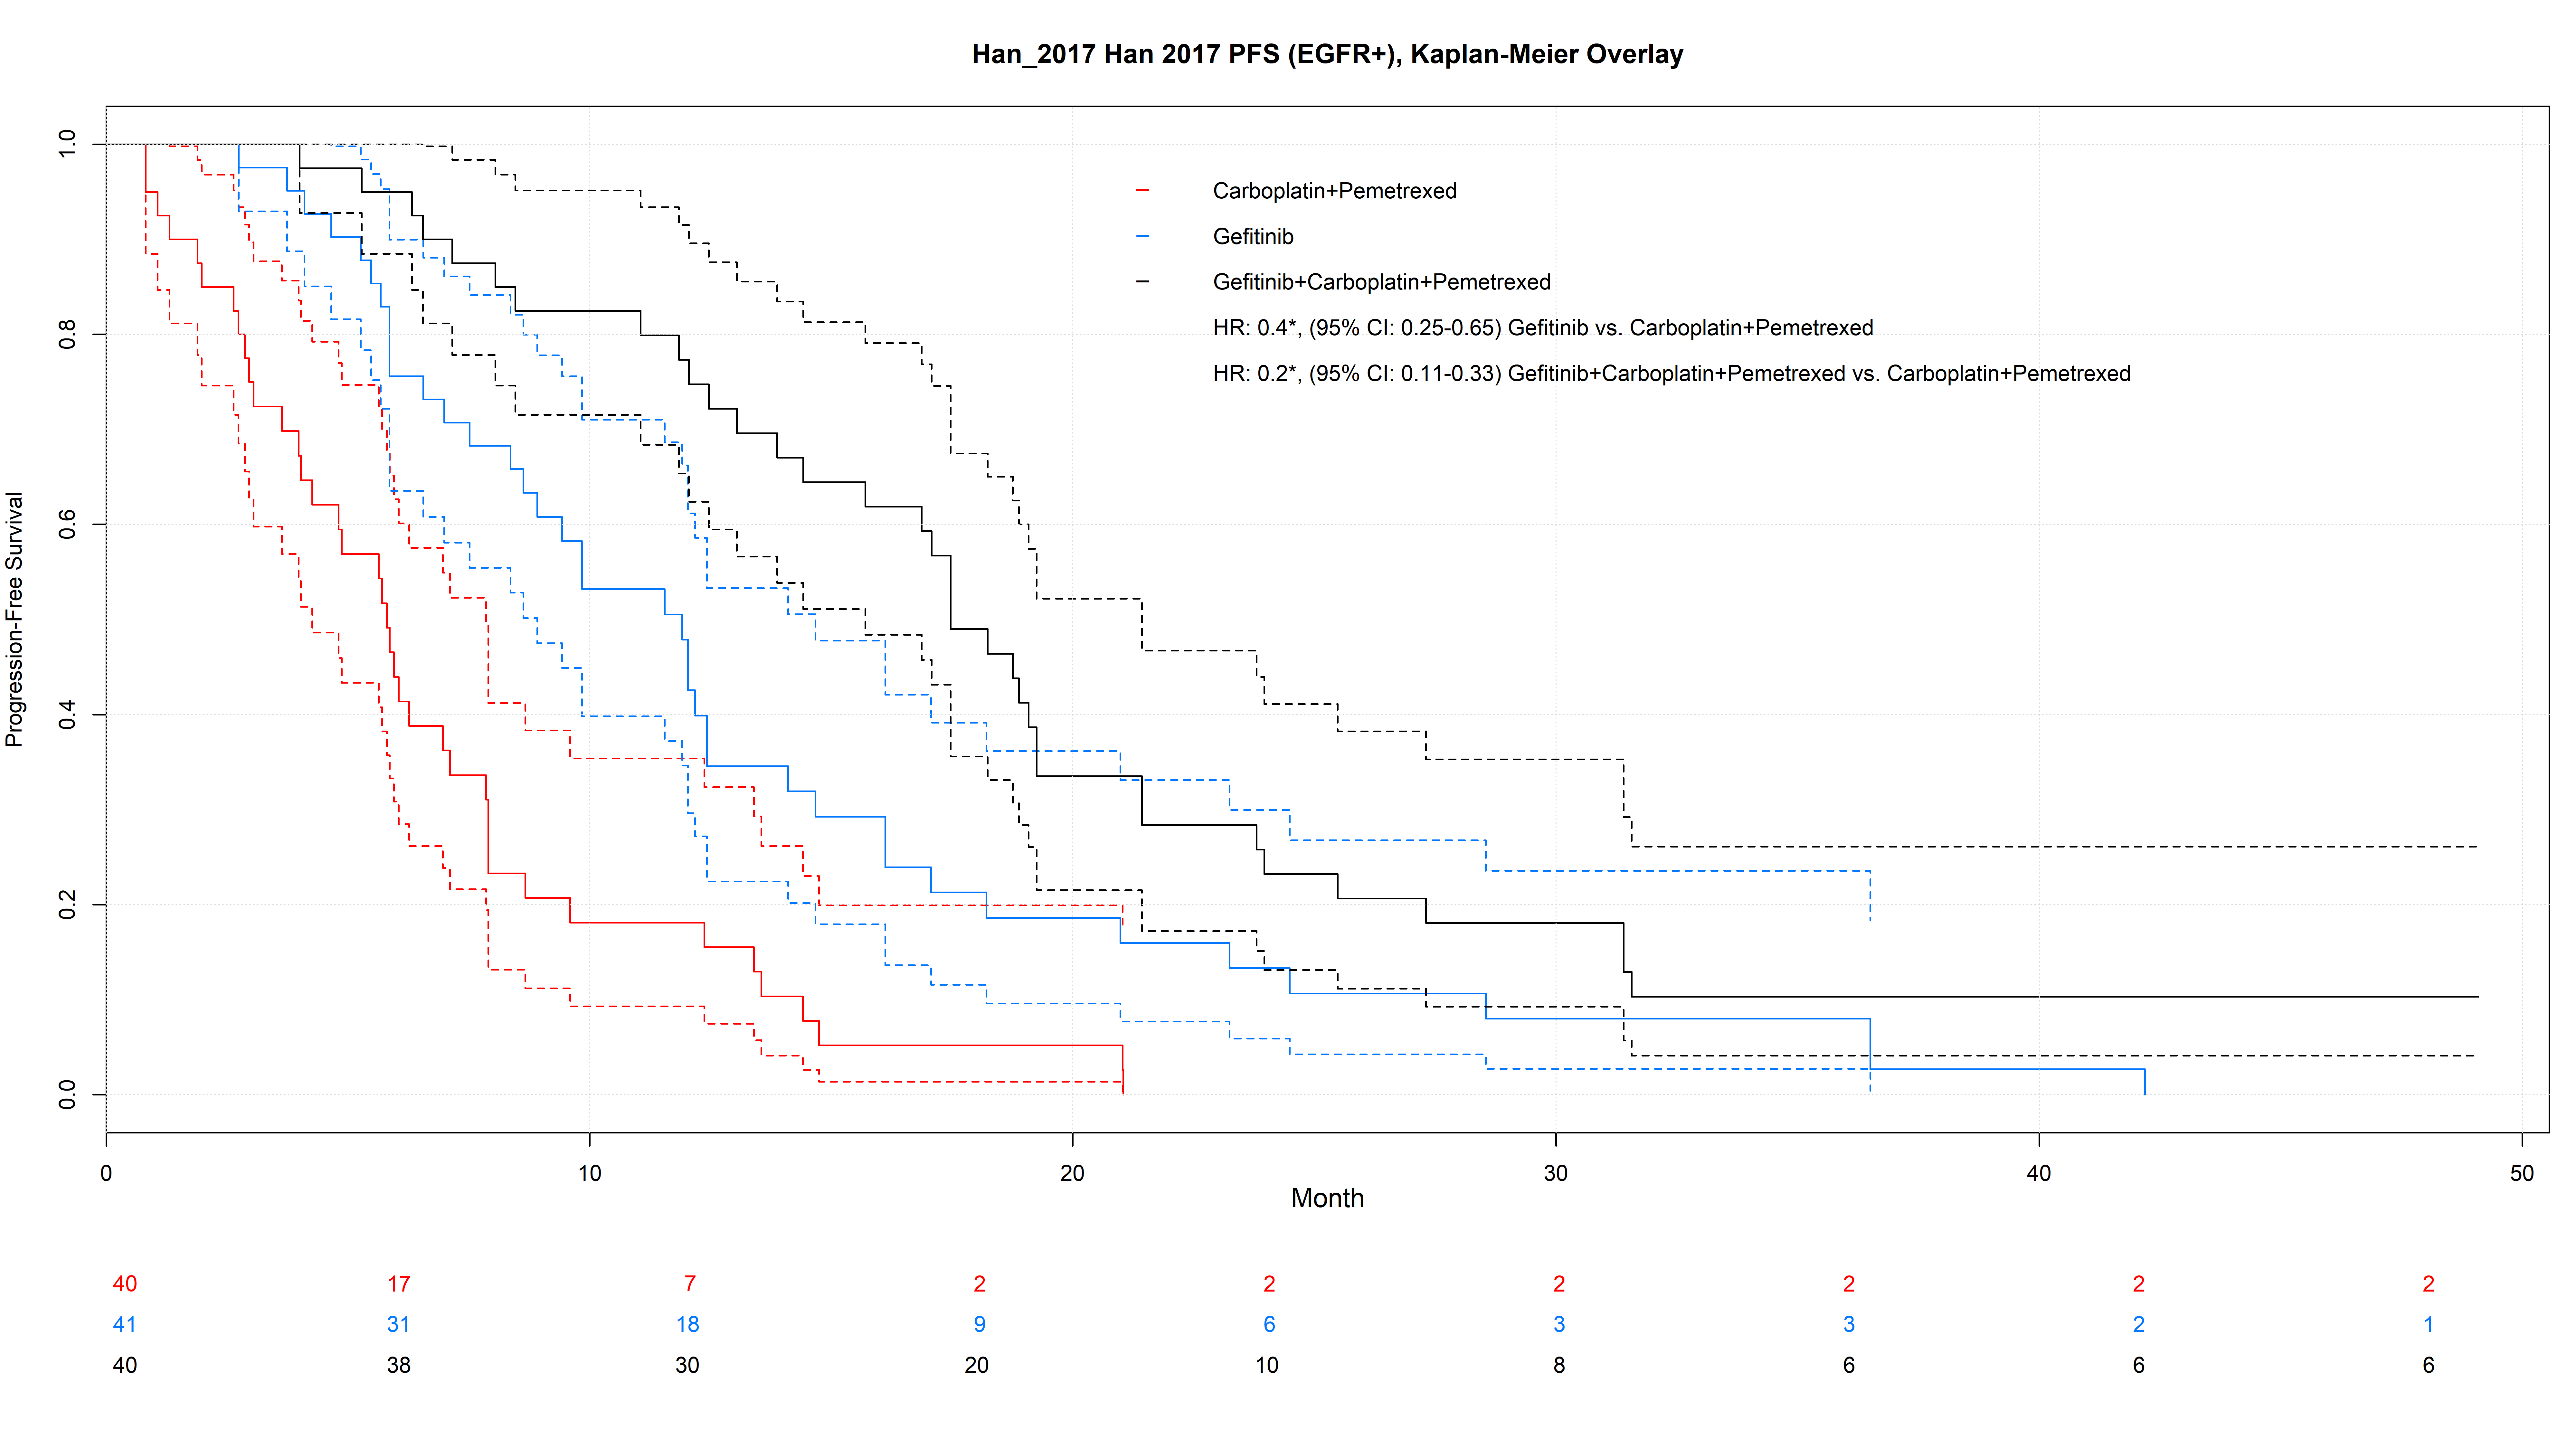
\includegraphics[max size={\textwidth}{\textheight}]{figs/km-plots/Han_2017 Han 2017 PFS (EGFR+) Kaplan Meier.png}
\end{subfigure}
\begin{subfigure}{\textwidth}
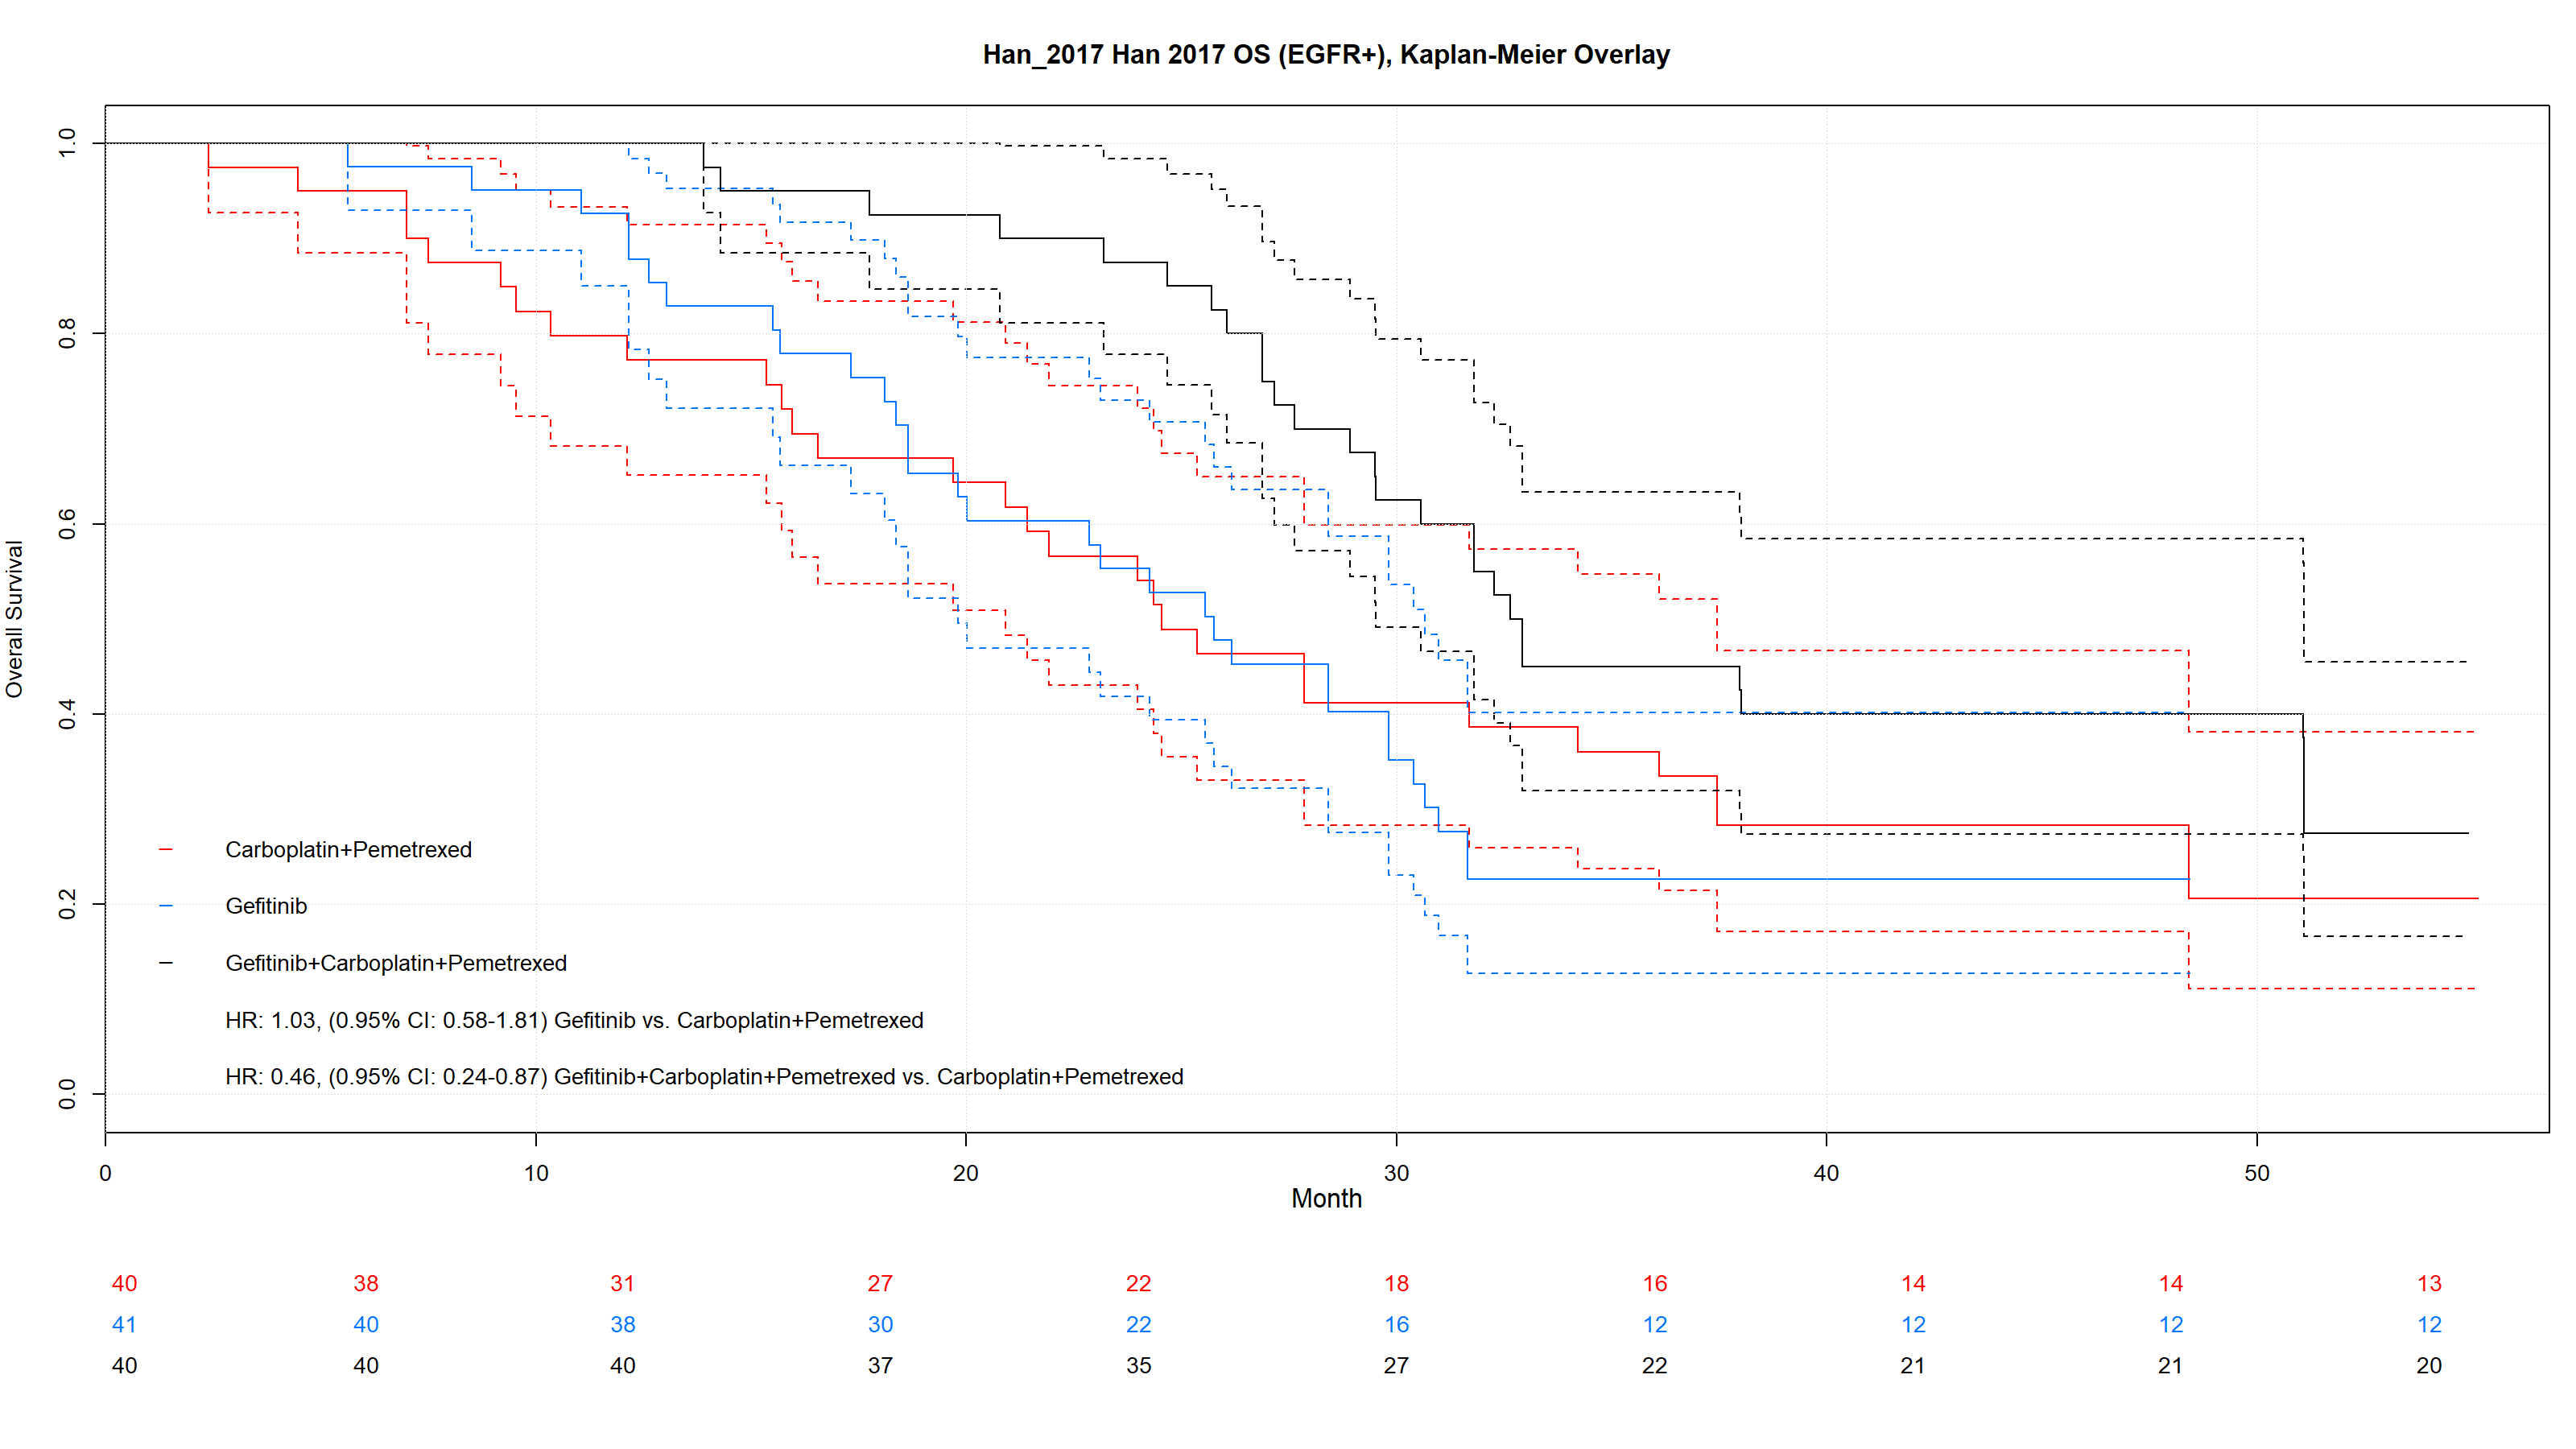
\includegraphics[max size={\textwidth}{\textheight}]{figs/km-plots/Han_2017 Han 2017 OS (EGFR+) Kaplan Meier.png}
\end{subfigure}
\centering
\caption{Han 2017, progression-free survival and overall survival}\label{fig:Han-2017}
\end{figure}


\begin{figure}
\centering
\begin{subfigure}{\textwidth}
\centering
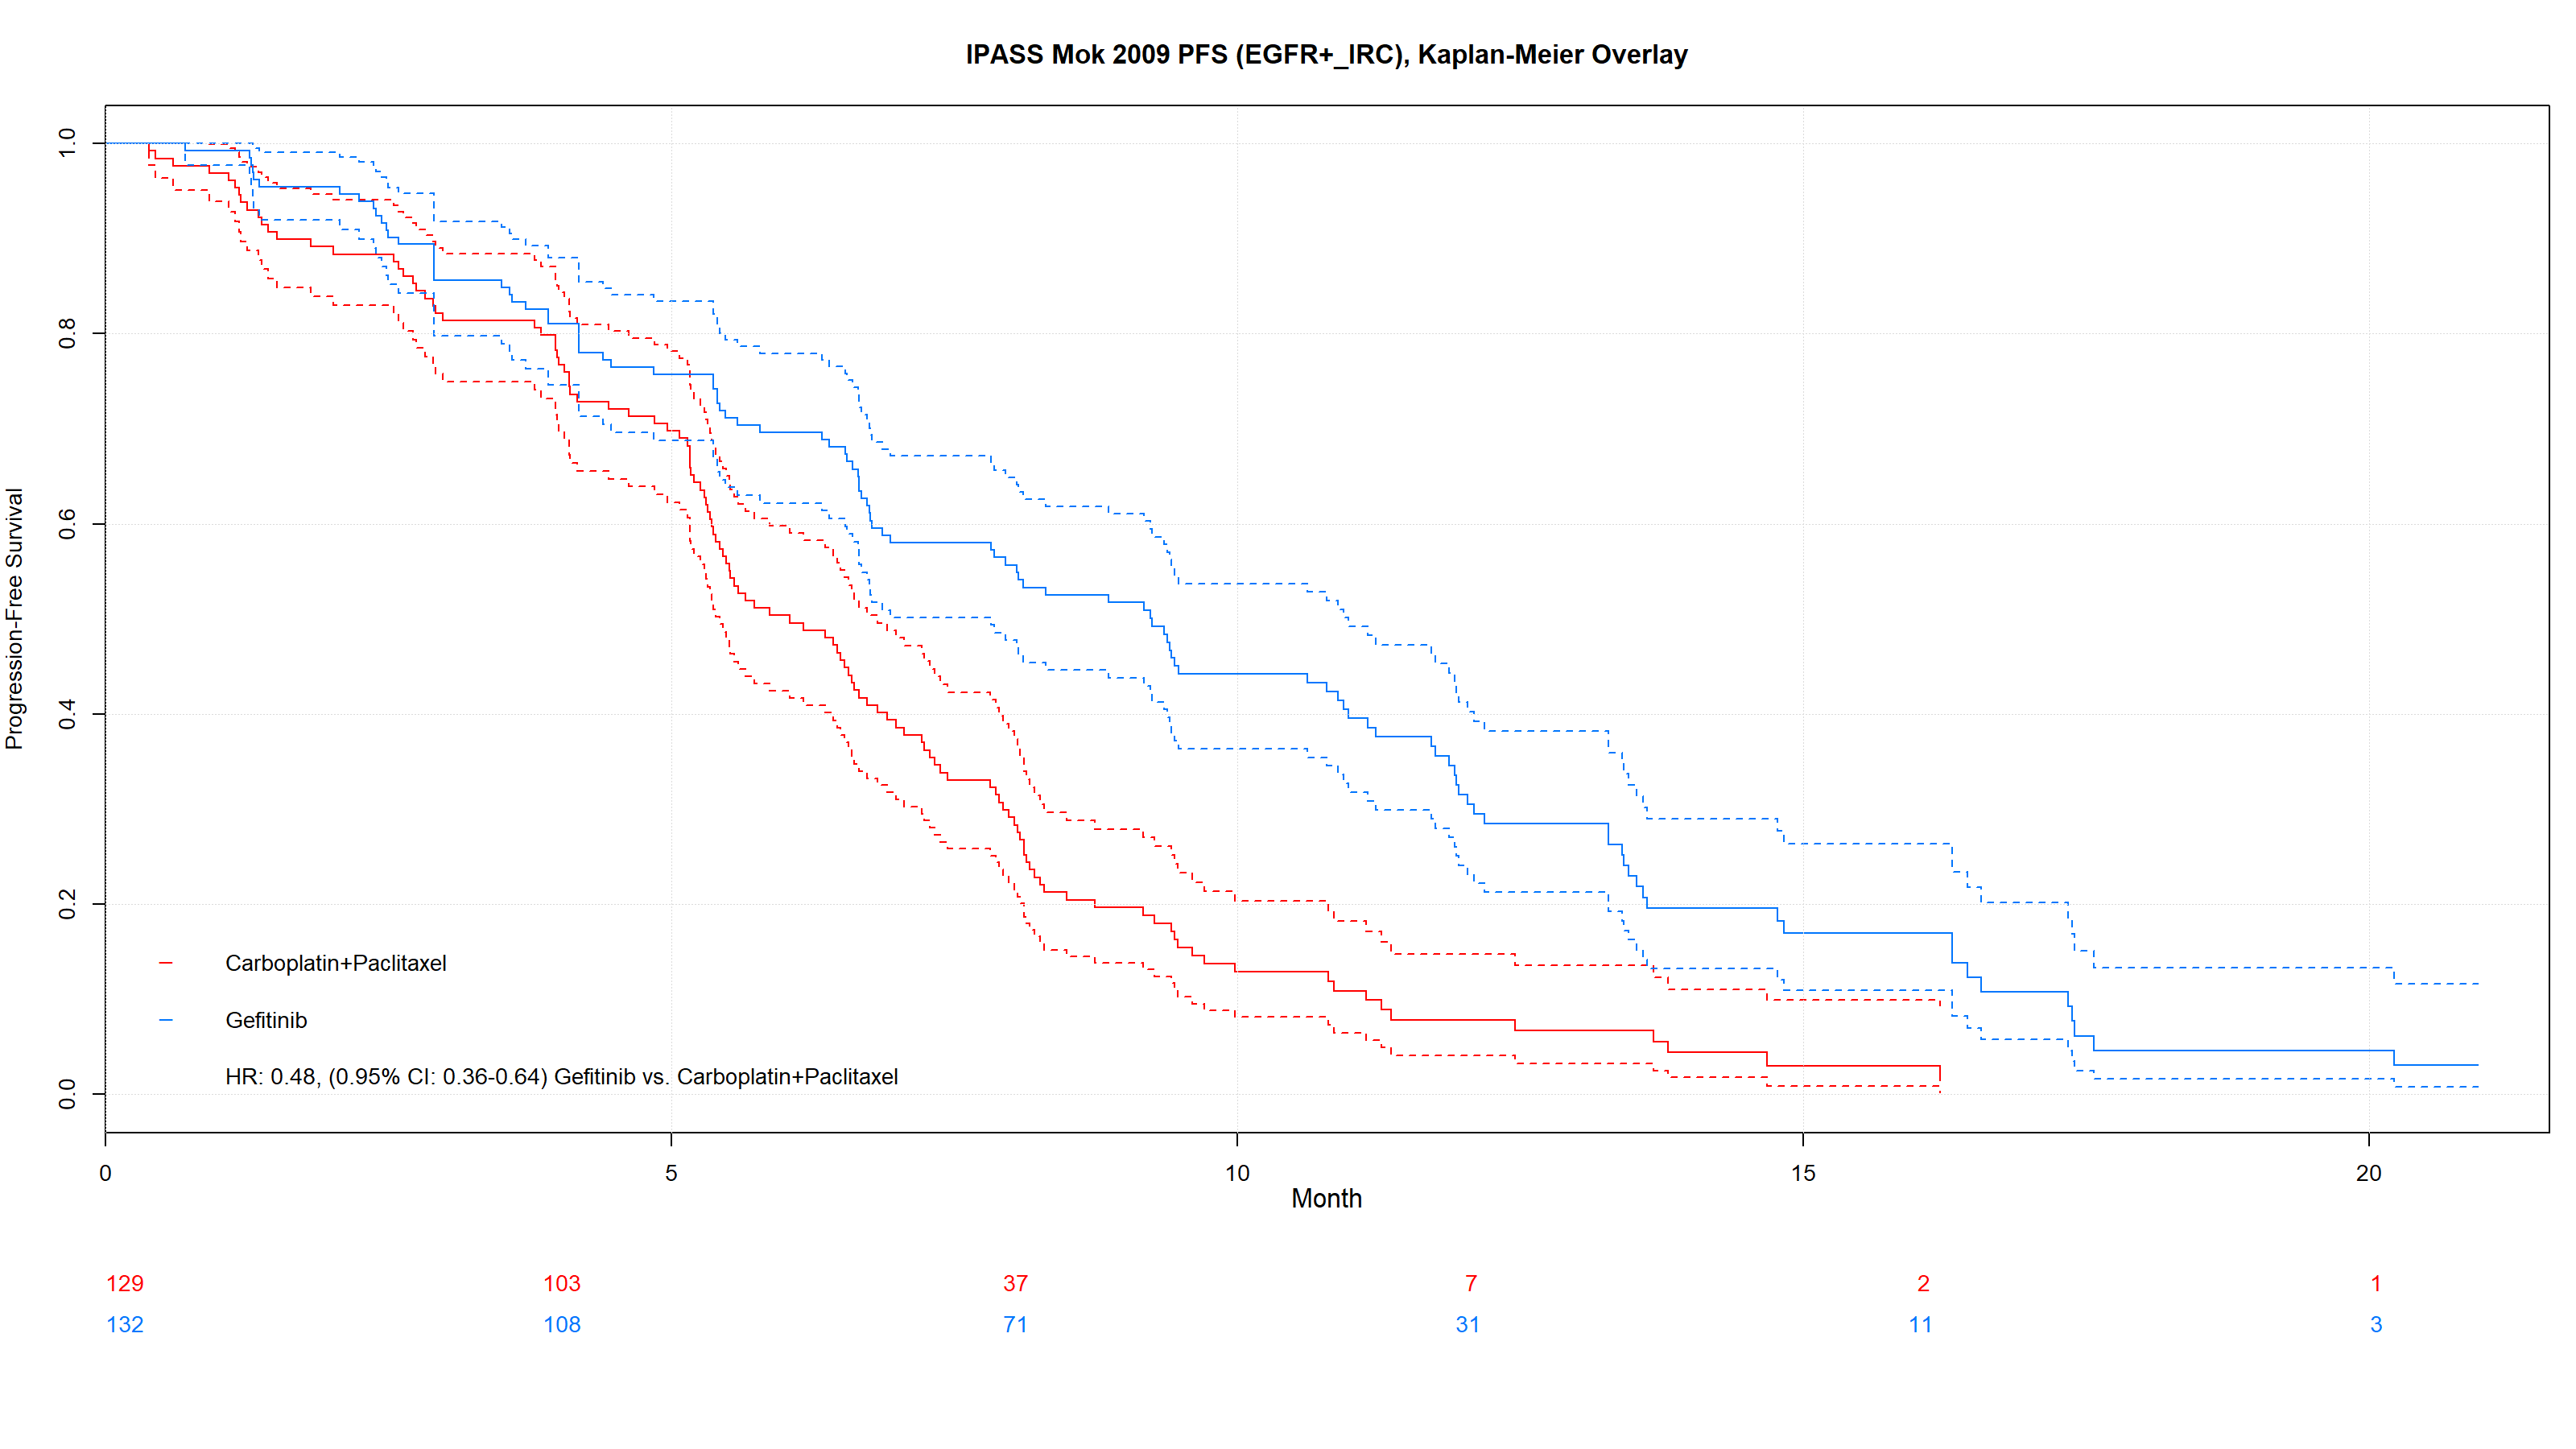
\includegraphics[max size={\textwidth}{\textheight}]{figs/km-plots/IPASS Mok 2009 PFS (EGFR+_IRC) Kaplan Meier.png}
\end{subfigure}
\begin{subfigure}{\textwidth}
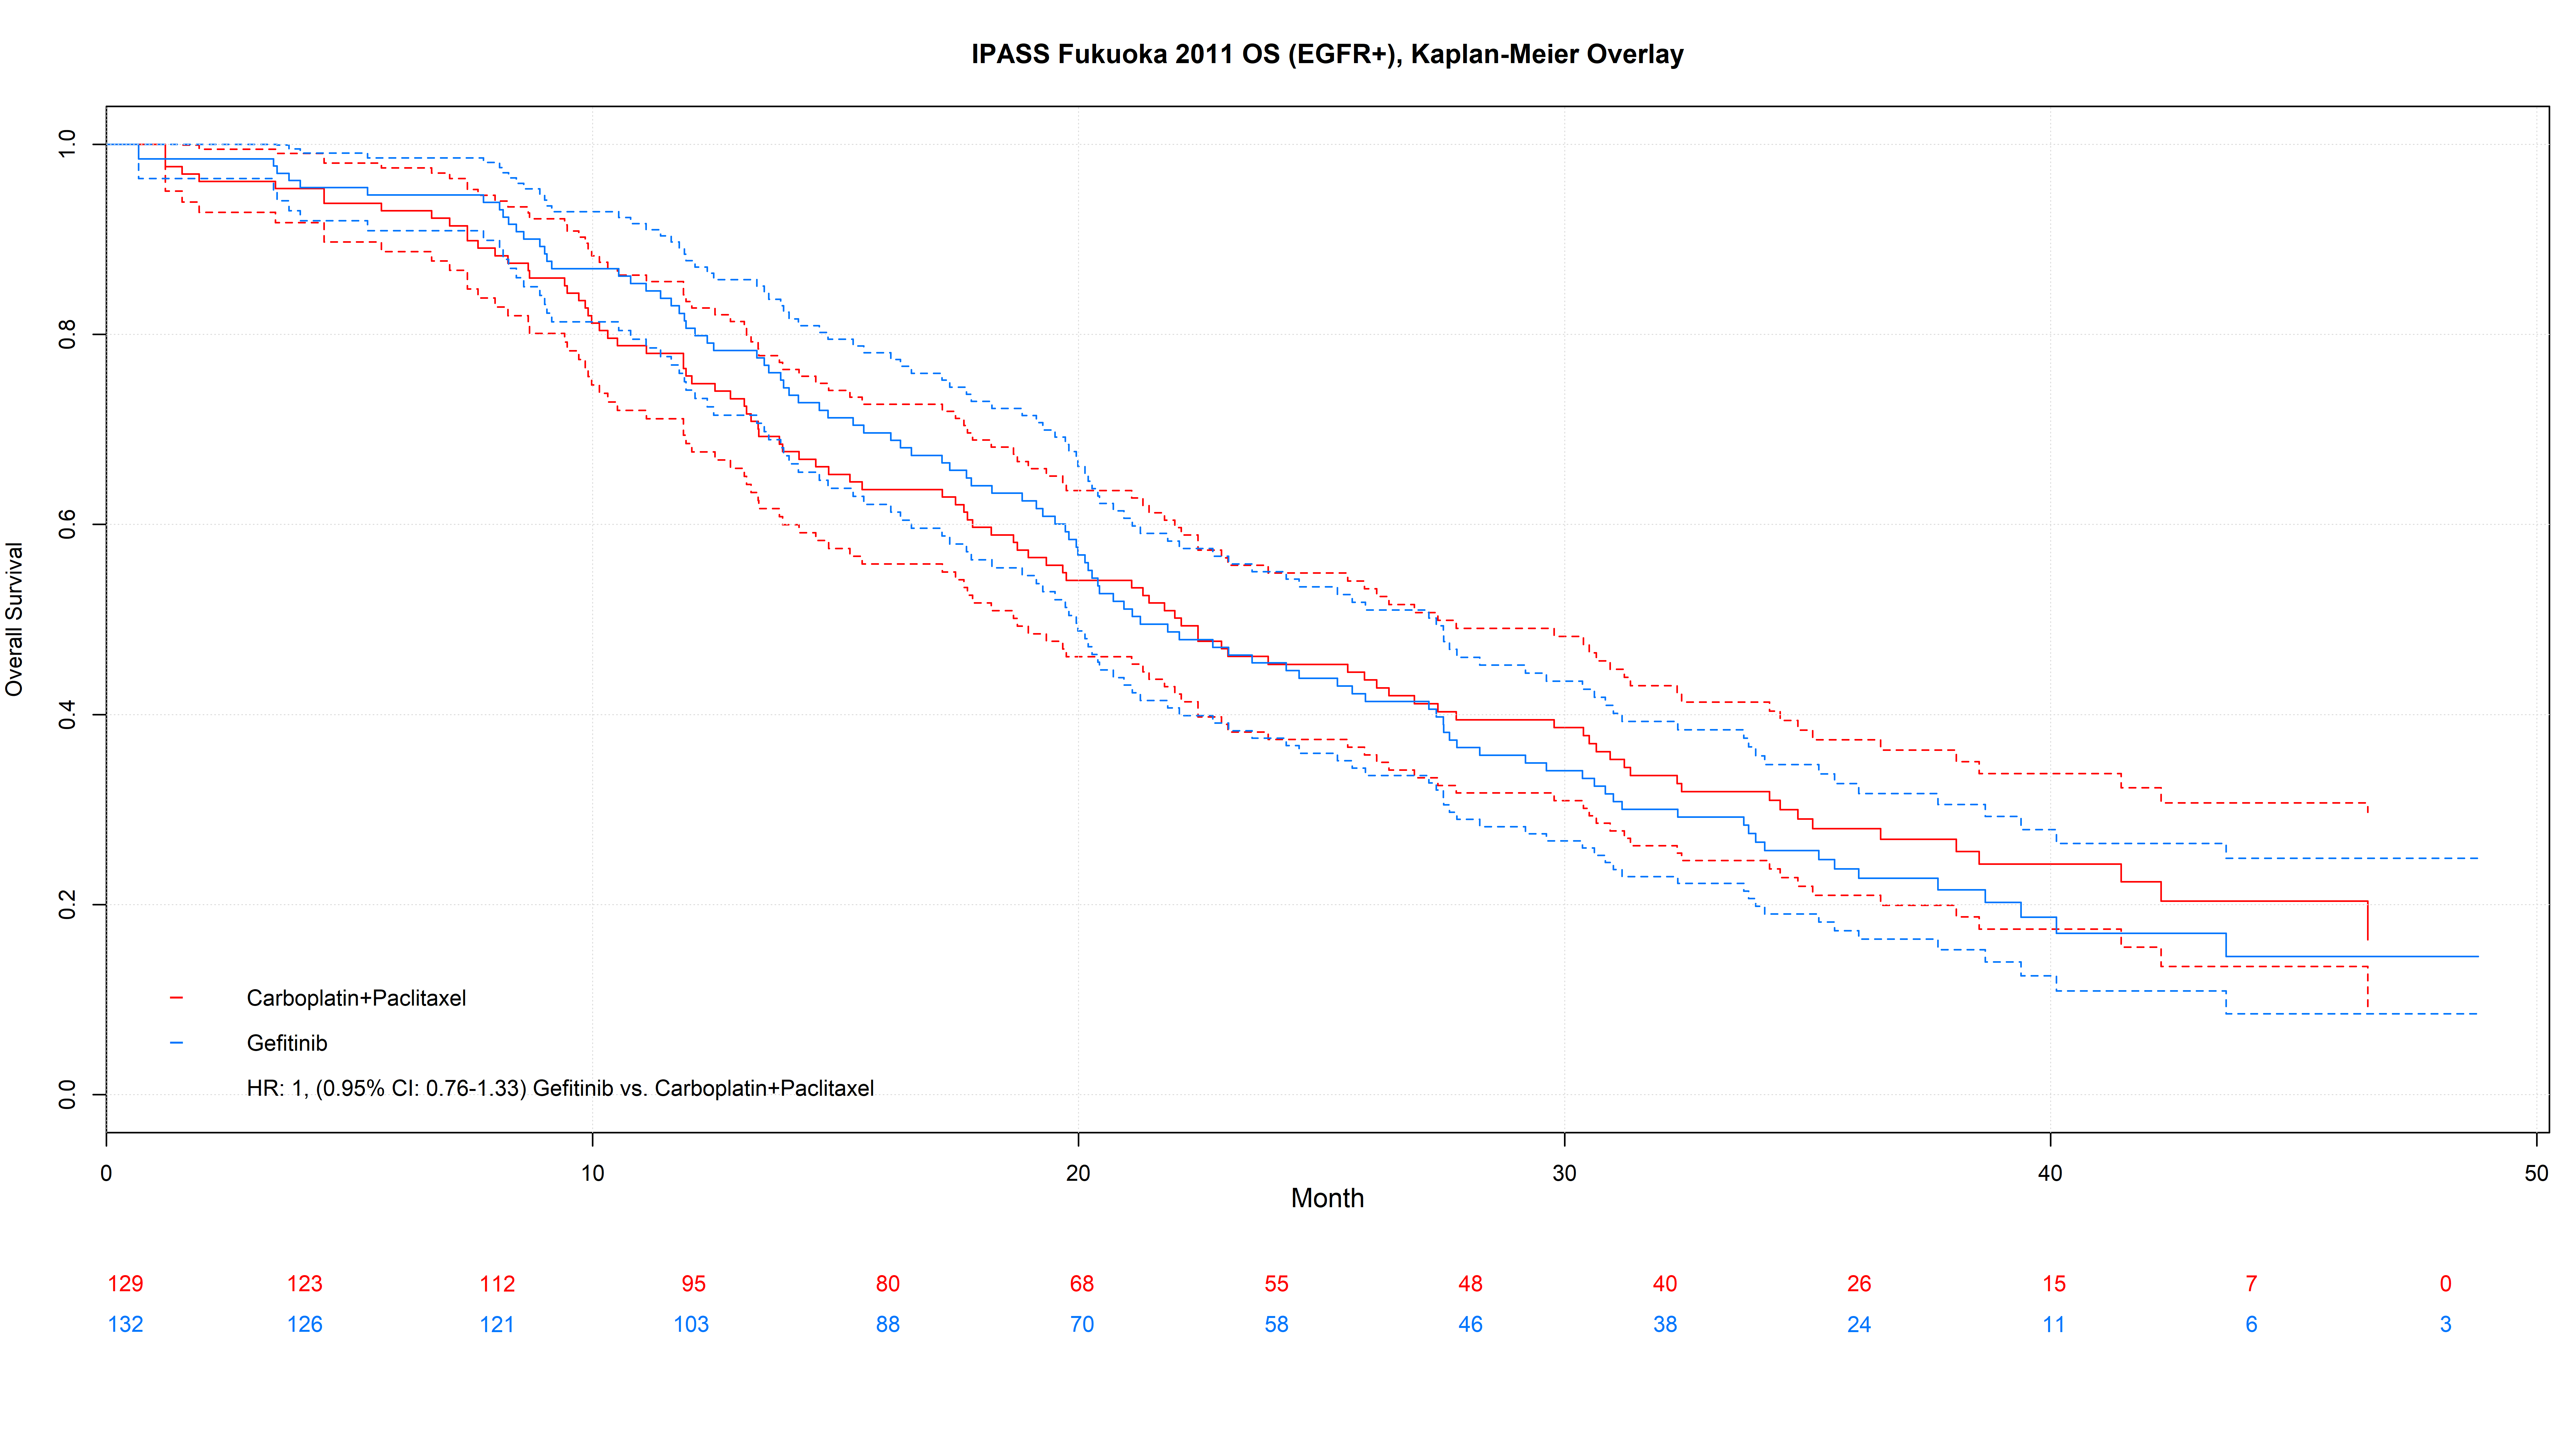
\includegraphics[max size={\textwidth}{\textheight}]{figs/km-plots/IPASS Fukuoka 2011 OS (EGFR+) Kaplan Meier.png}
\end{subfigure}
\centering
\caption{IPASS, progression-free survival and overall survival}\label{fig:IPASS}
\end{figure}


\begin{figure}
\centering
\begin{subfigure}{\textwidth}
\centering
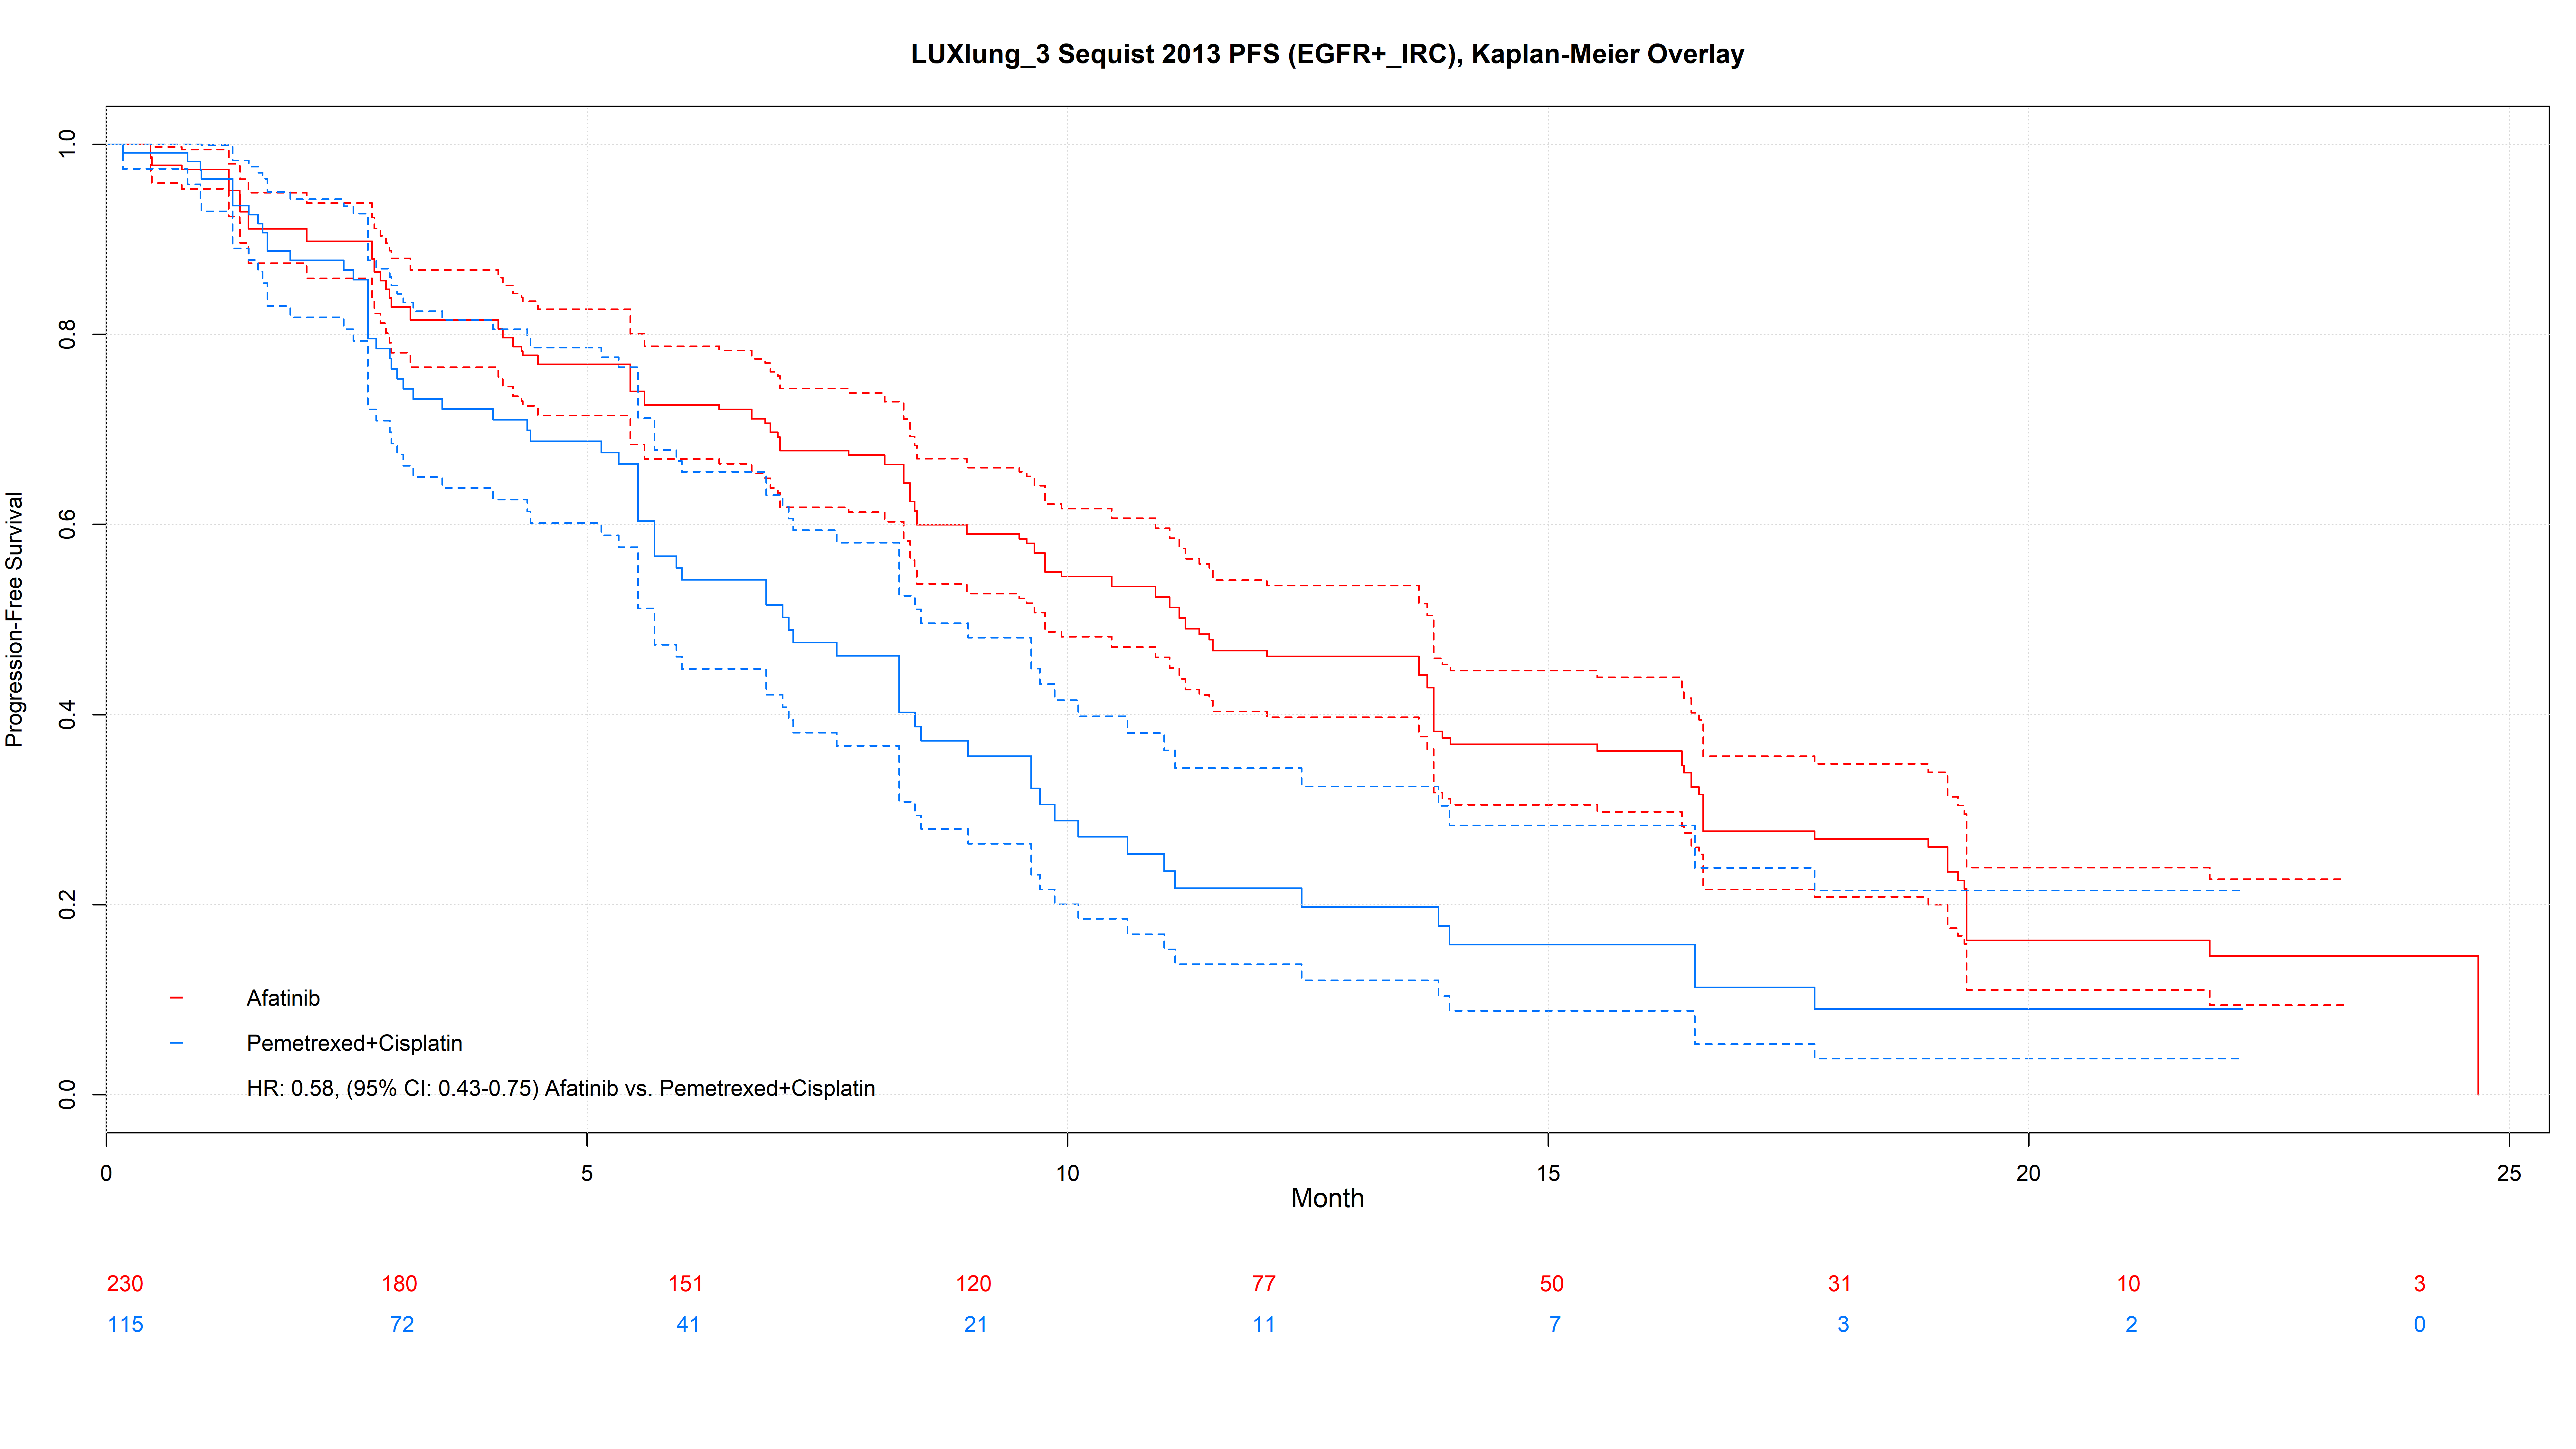
\includegraphics[max size={\textwidth}{\textheight}]{figs/km-plots/LUXlung_3 Sequist 2013 PFS (EGFR+_IRC) Kaplan Meier.png}
\end{subfigure}
\begin{subfigure}{\textwidth}
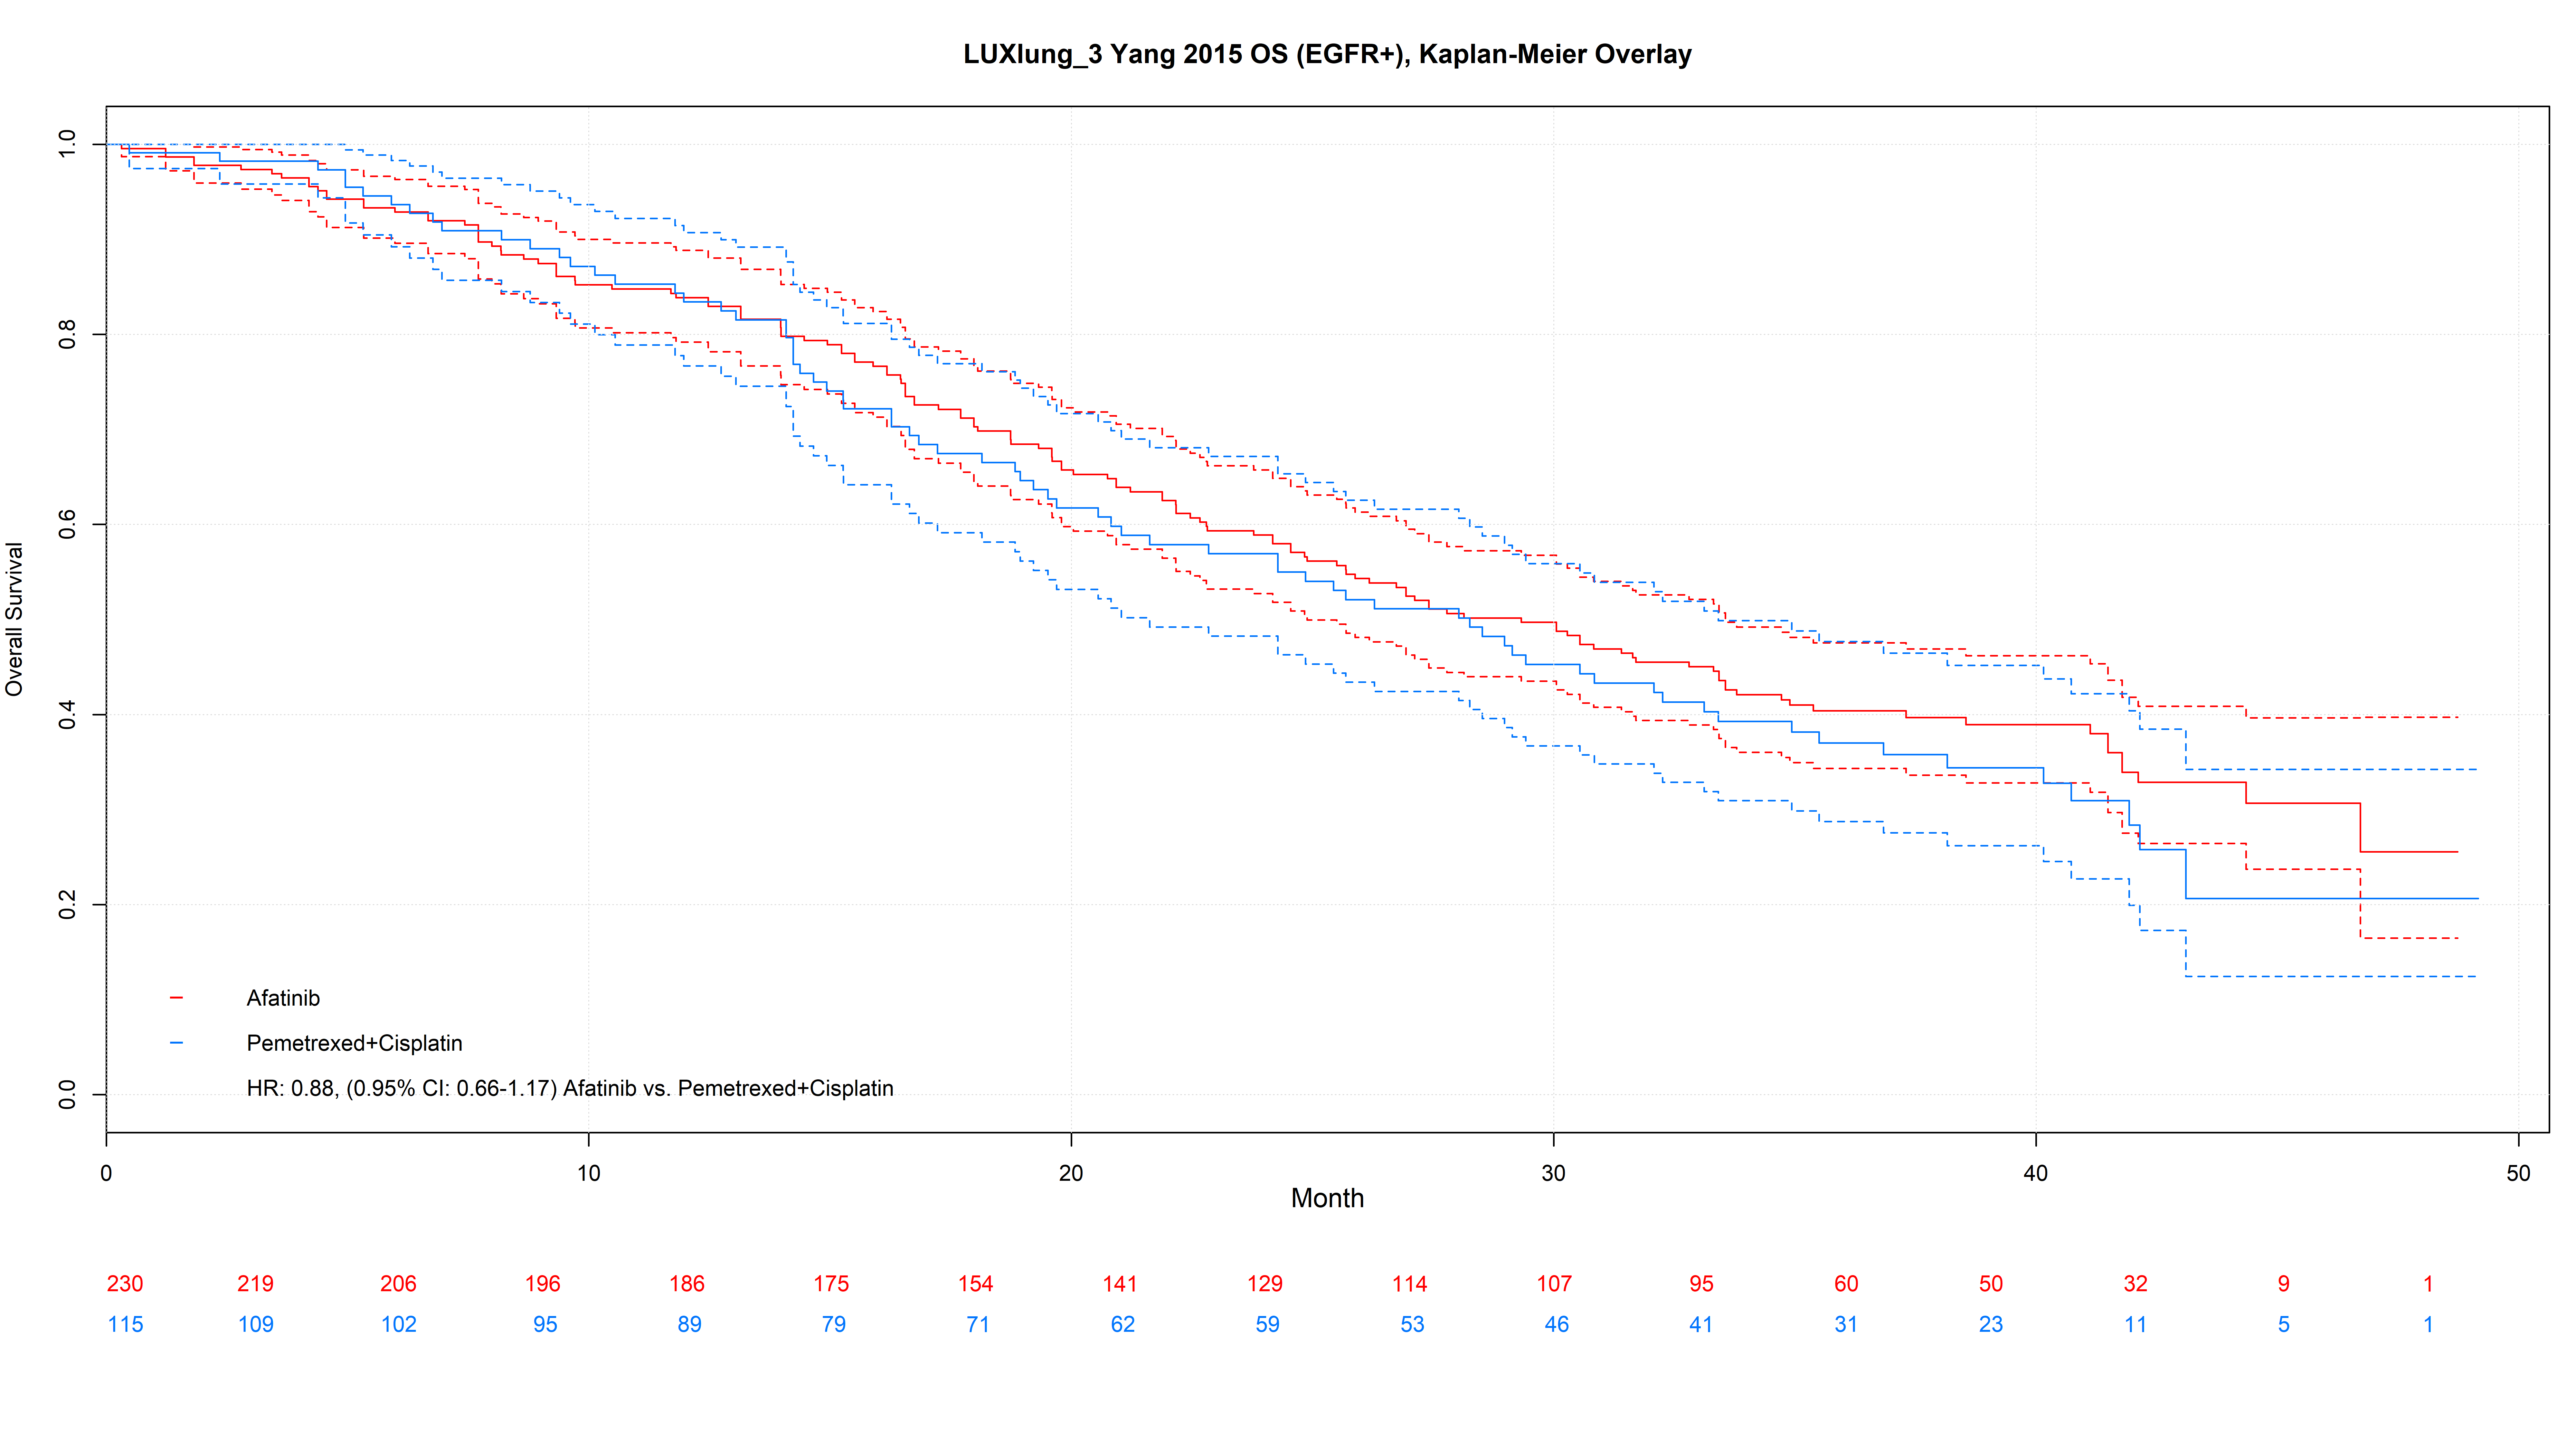
\includegraphics[max size={\textwidth}{\textheight}]{figs/km-plots/LUXlung_3 Yang 2015 OS (EGFR+) Kaplan Meier.png}
\end{subfigure}
\centering
\caption{LUX-LUNG 3, progression-free survival and overall survival}\label{fig:LUX-LUNG 3}
\end{figure}


\begin{figure}
\centering
\begin{subfigure}{\textwidth}
\centering
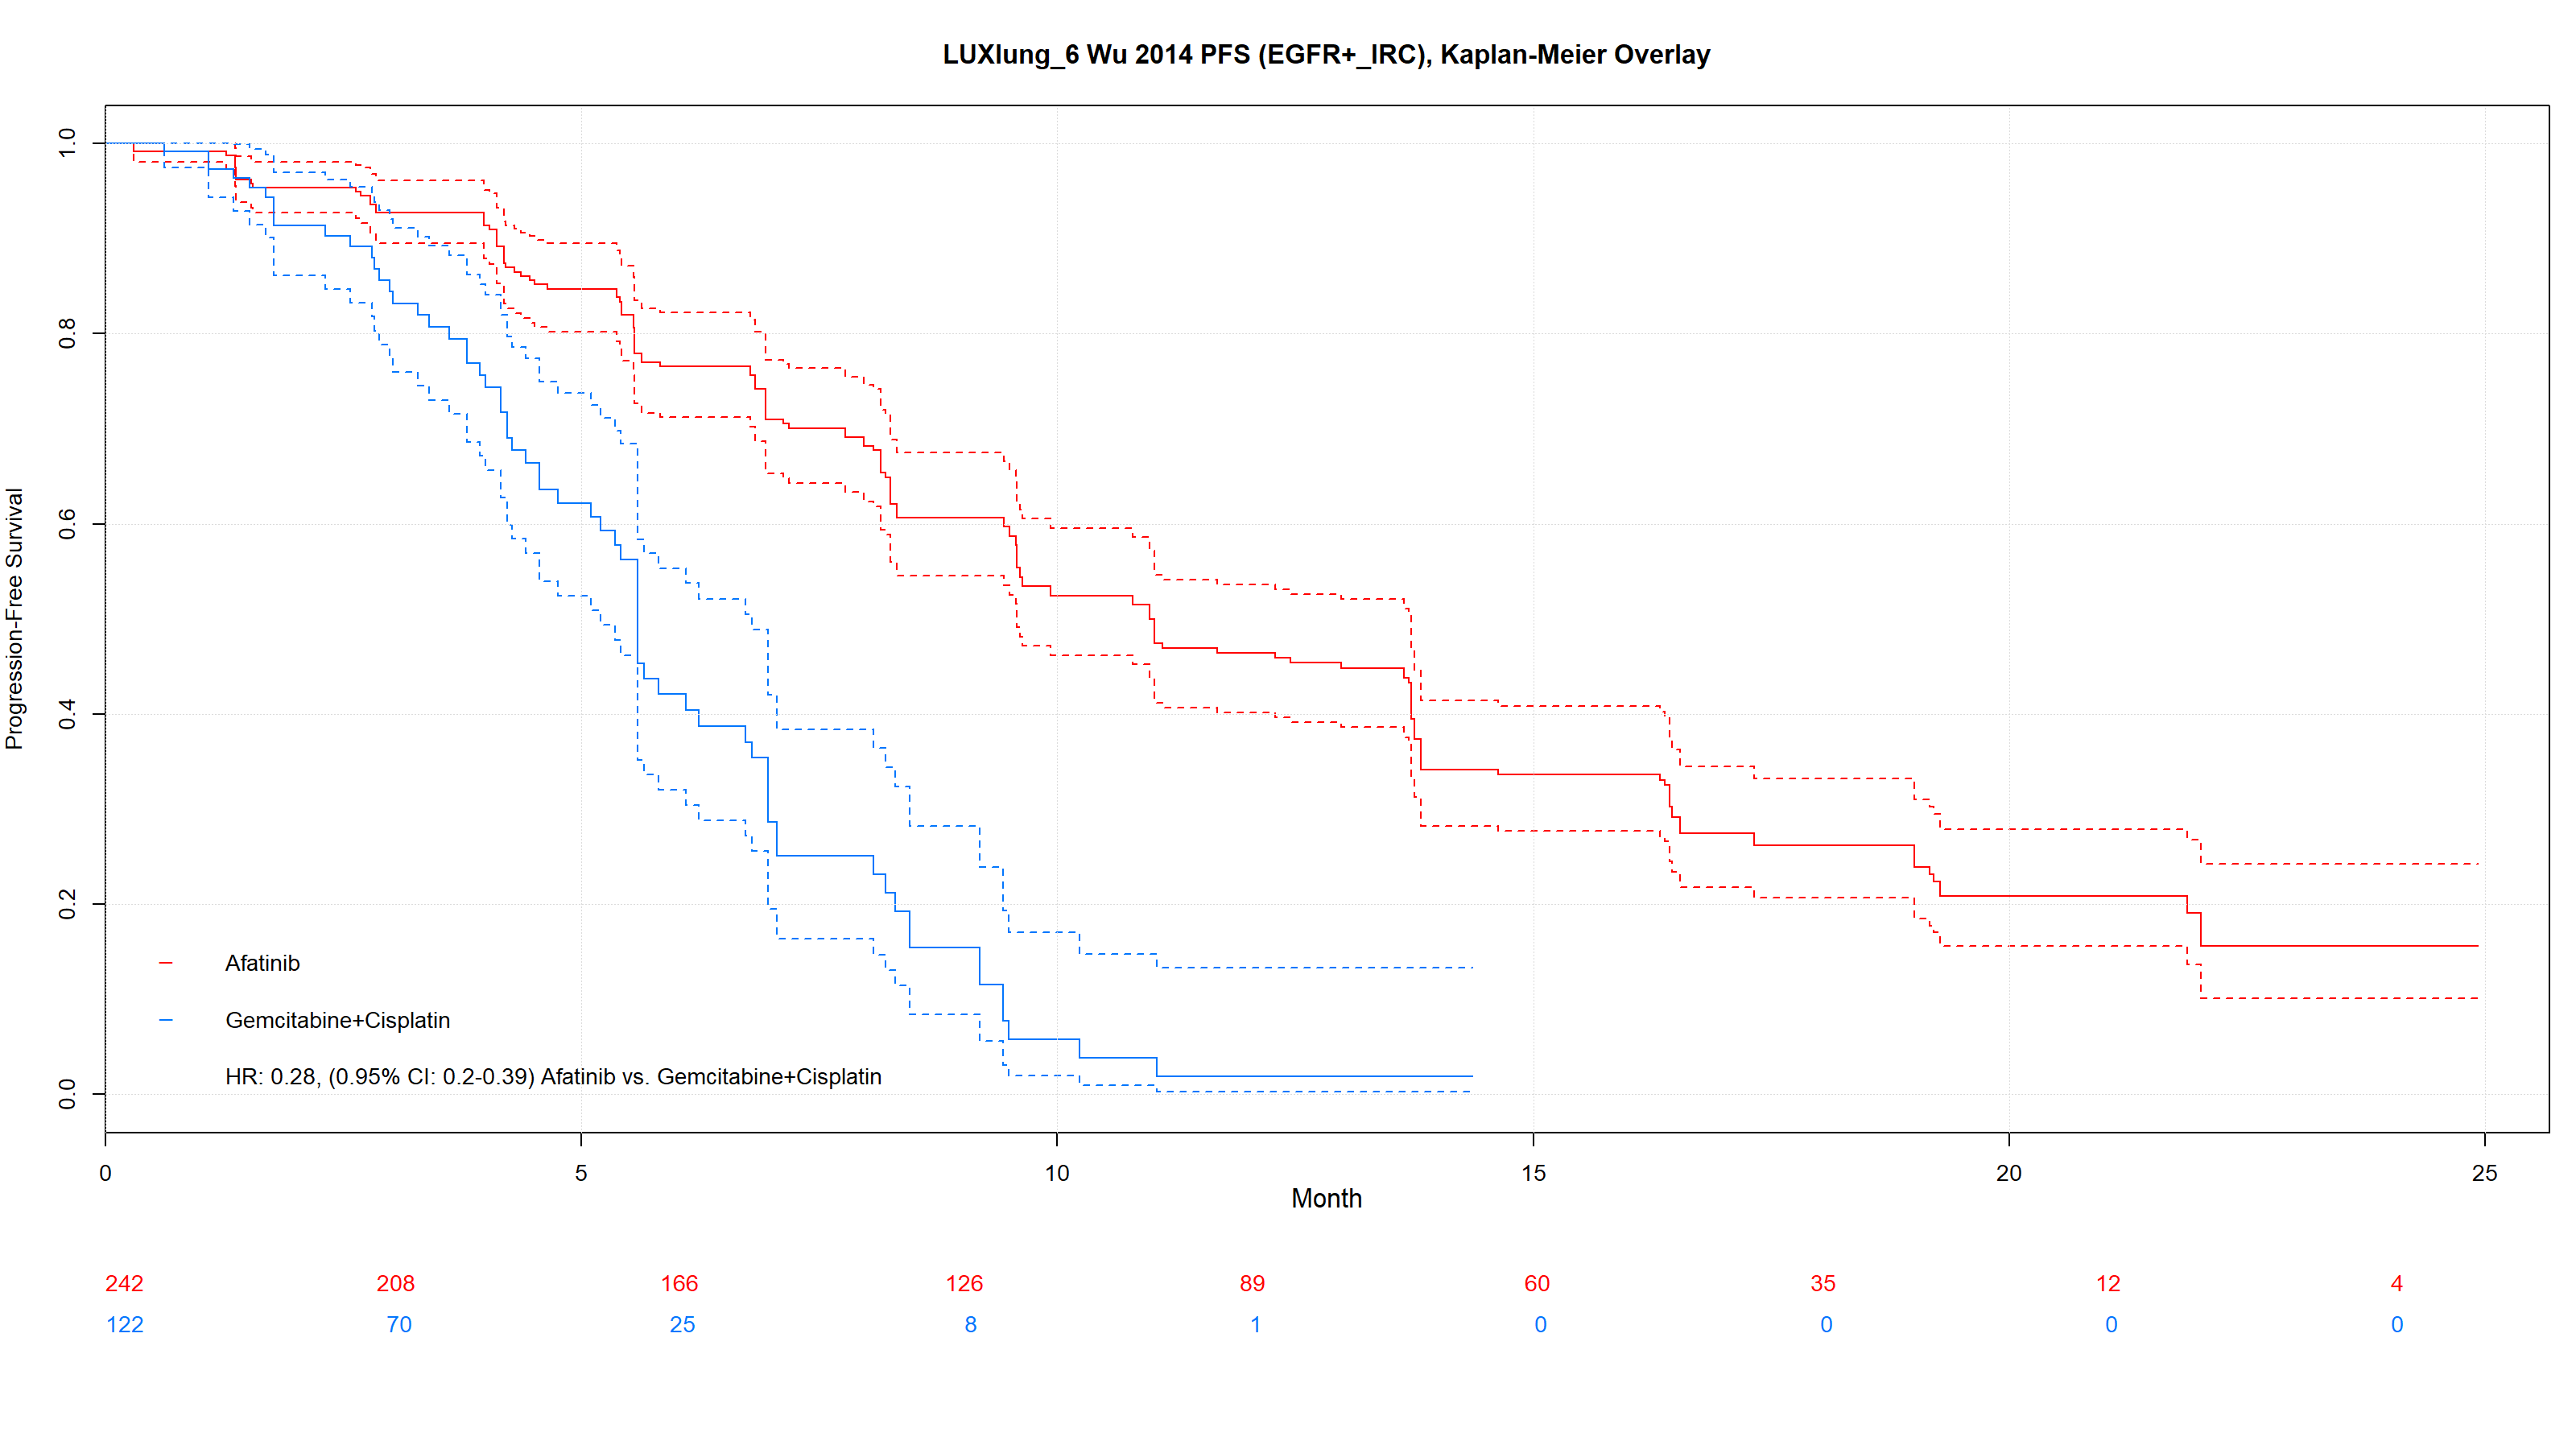
\includegraphics[max size={\textwidth}{\textheight}]{figs/km-plots/LUXlung_6 Wu 2014 PFS (EGFR+_IRC) Kaplan Meier.png}
\end{subfigure}
\begin{subfigure}{\textwidth}
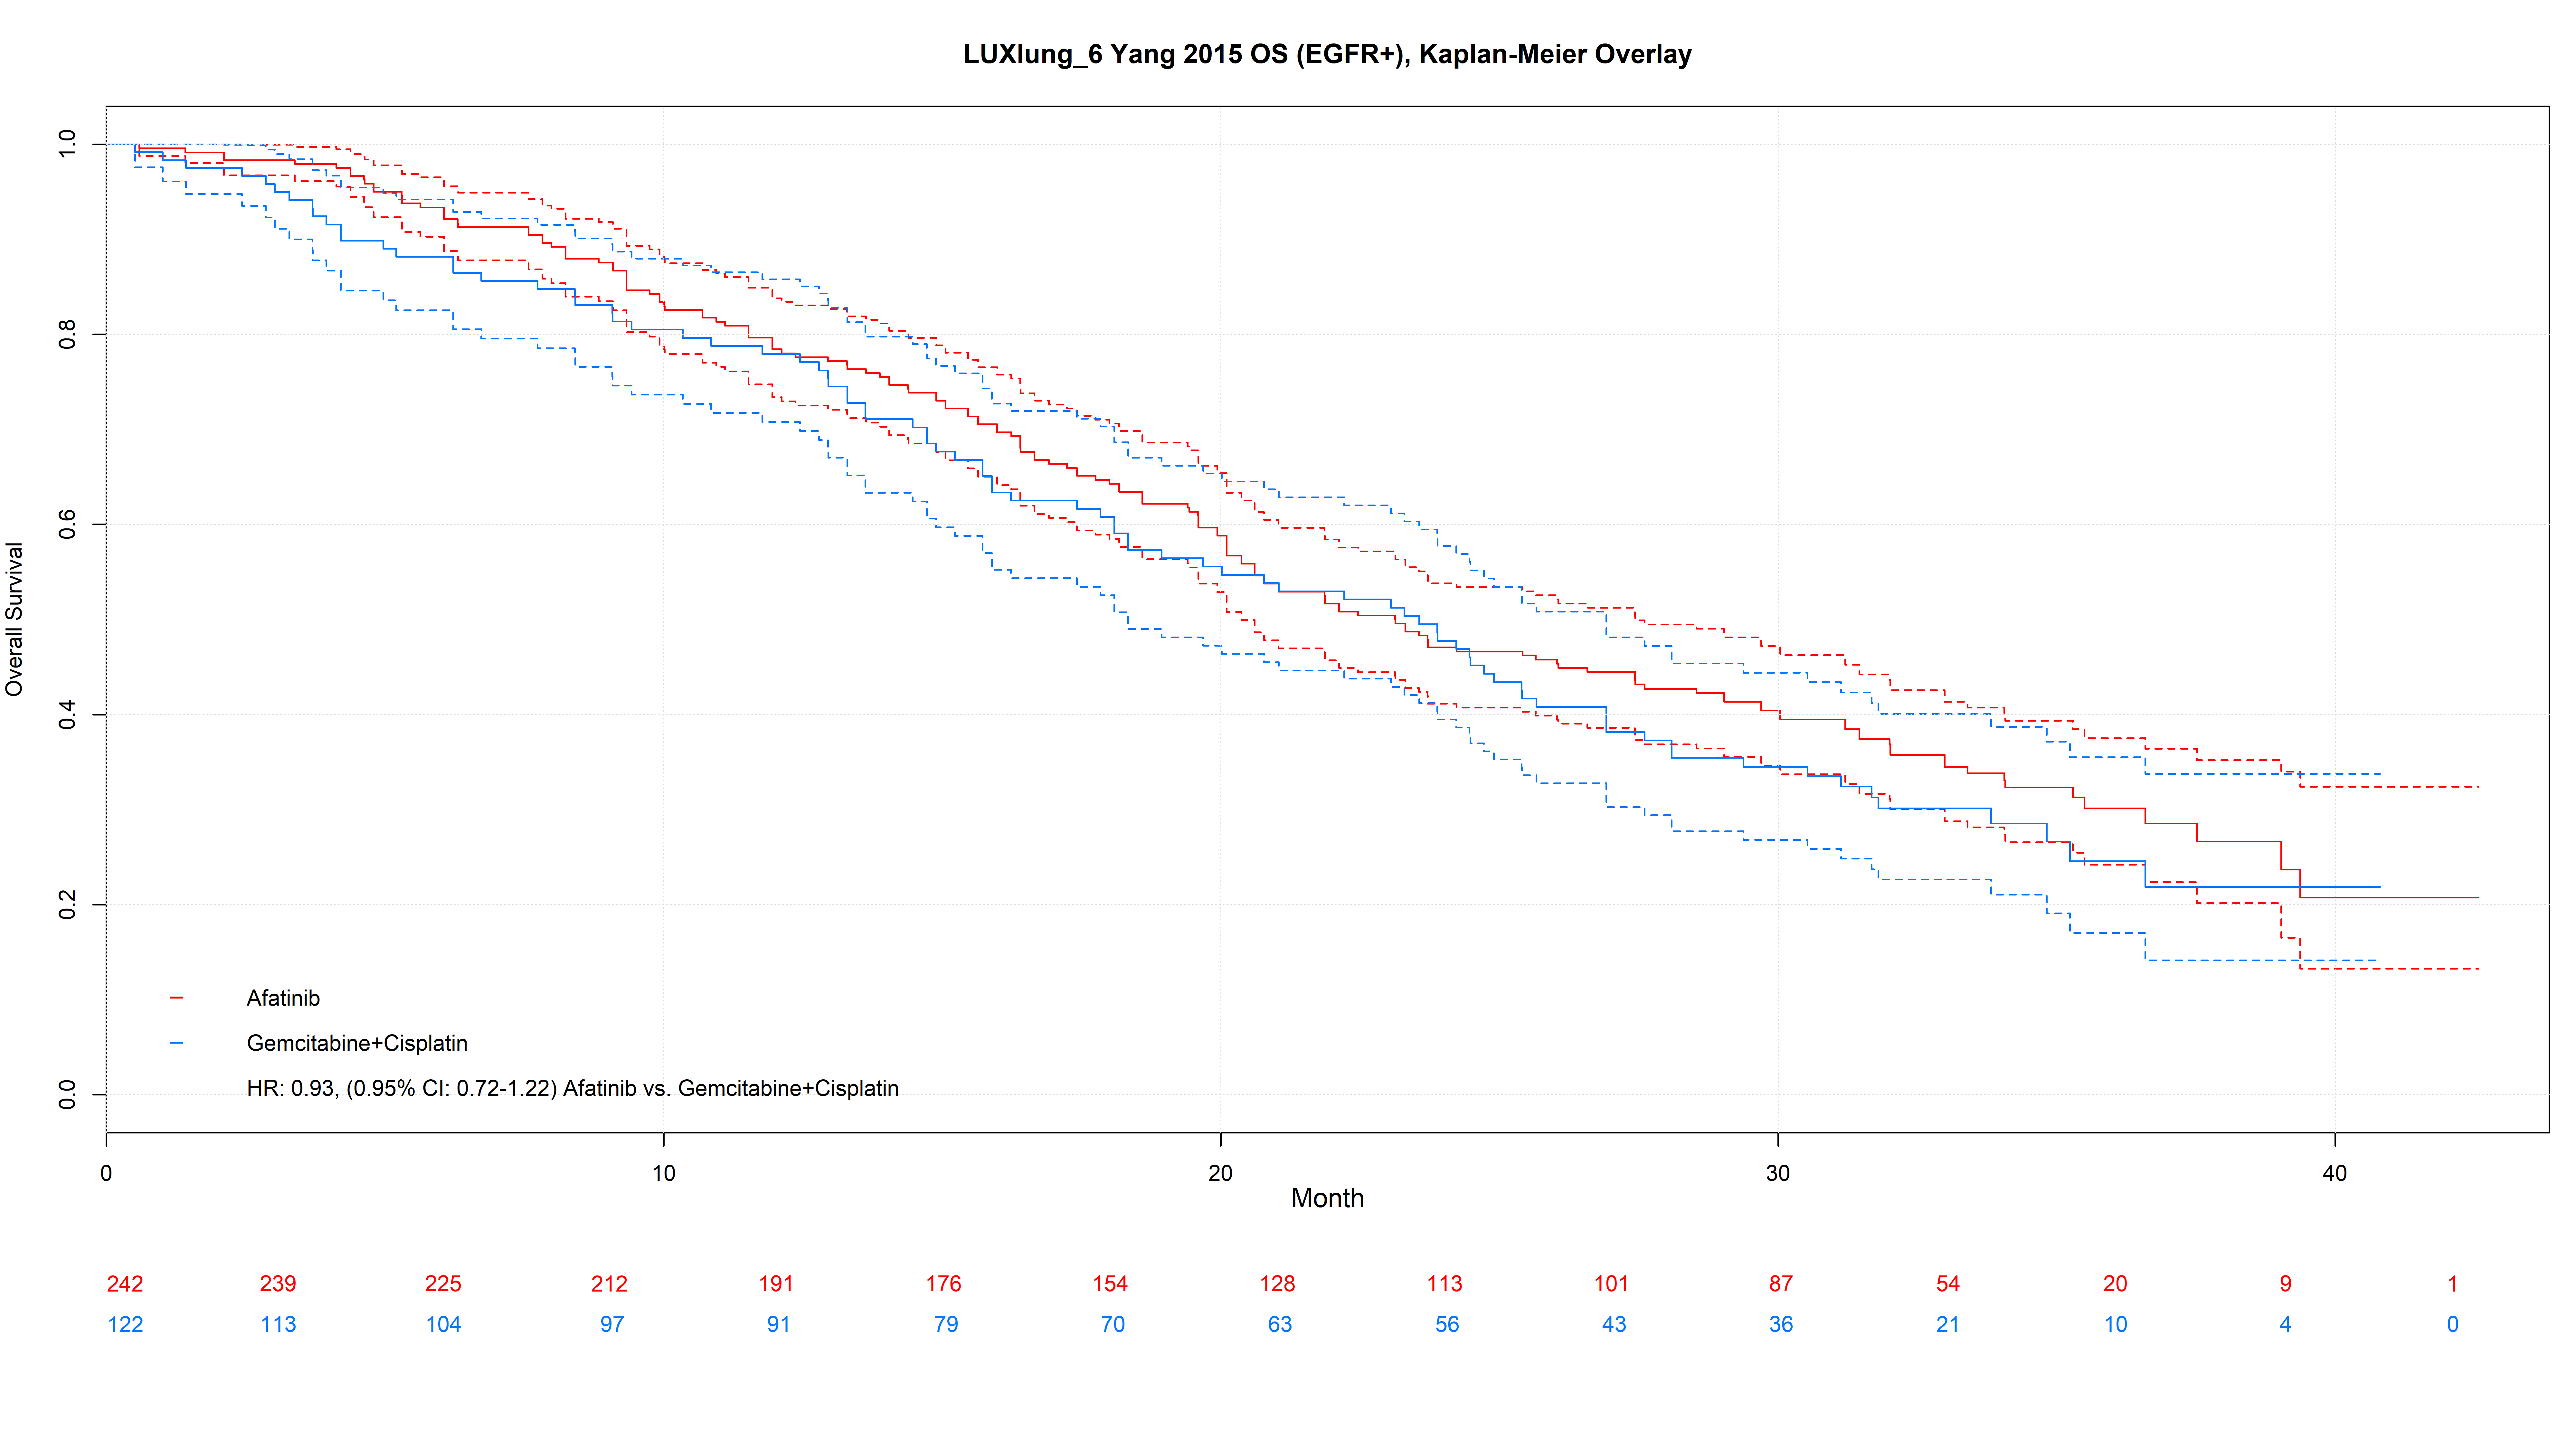
\includegraphics[max size={\textwidth}{\textheight}]{figs/km-plots/LUXlung_6 Yang 2015 OS (EGFR+) Kaplan Meier.png}
\end{subfigure}
\centering
\caption{LUX-LUNG 6, progression-free survival and overall survival}\label{fig:LUX-LUNG 6}
\end{figure}


\begin{figure}
\centering
\begin{subfigure}{\textwidth}
\centering
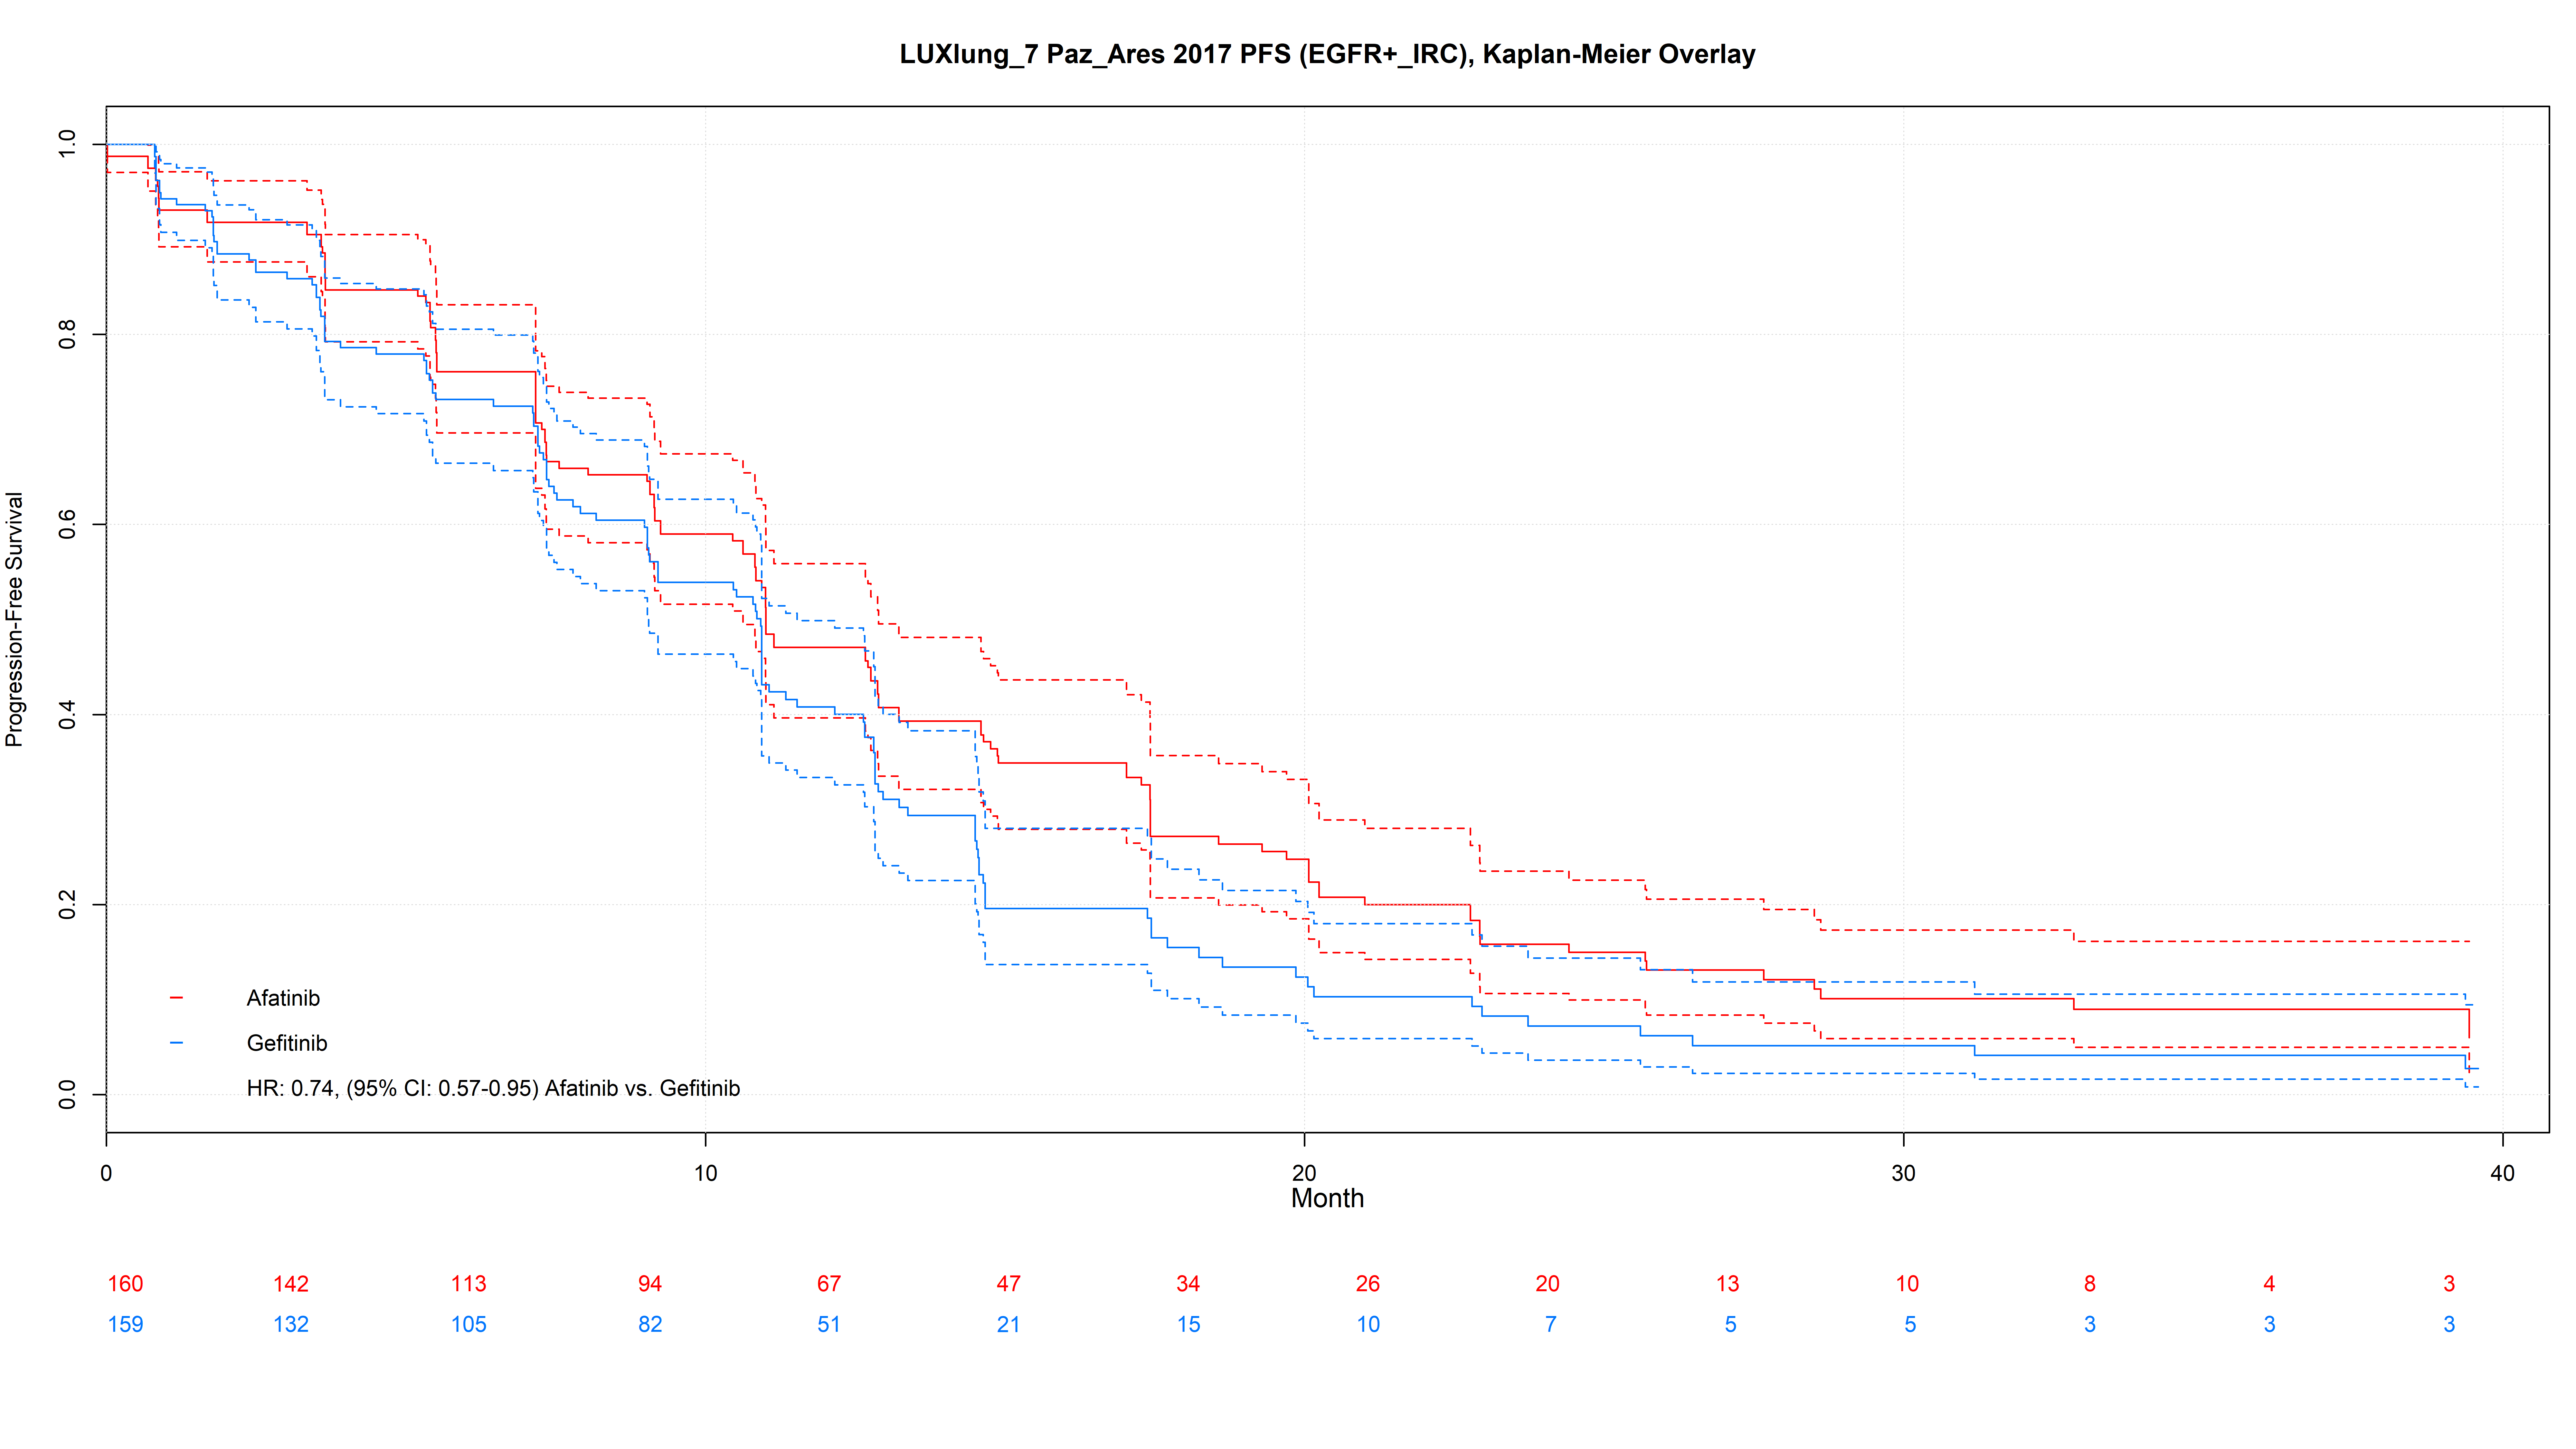
\includegraphics[max size={\textwidth}{\textheight}]{figs/km-plots/LUXlung_7 Paz_Ares 2017 PFS (EGFR+_IRC) Kaplan Meier.png}
\end{subfigure}
\begin{subfigure}{\textwidth}
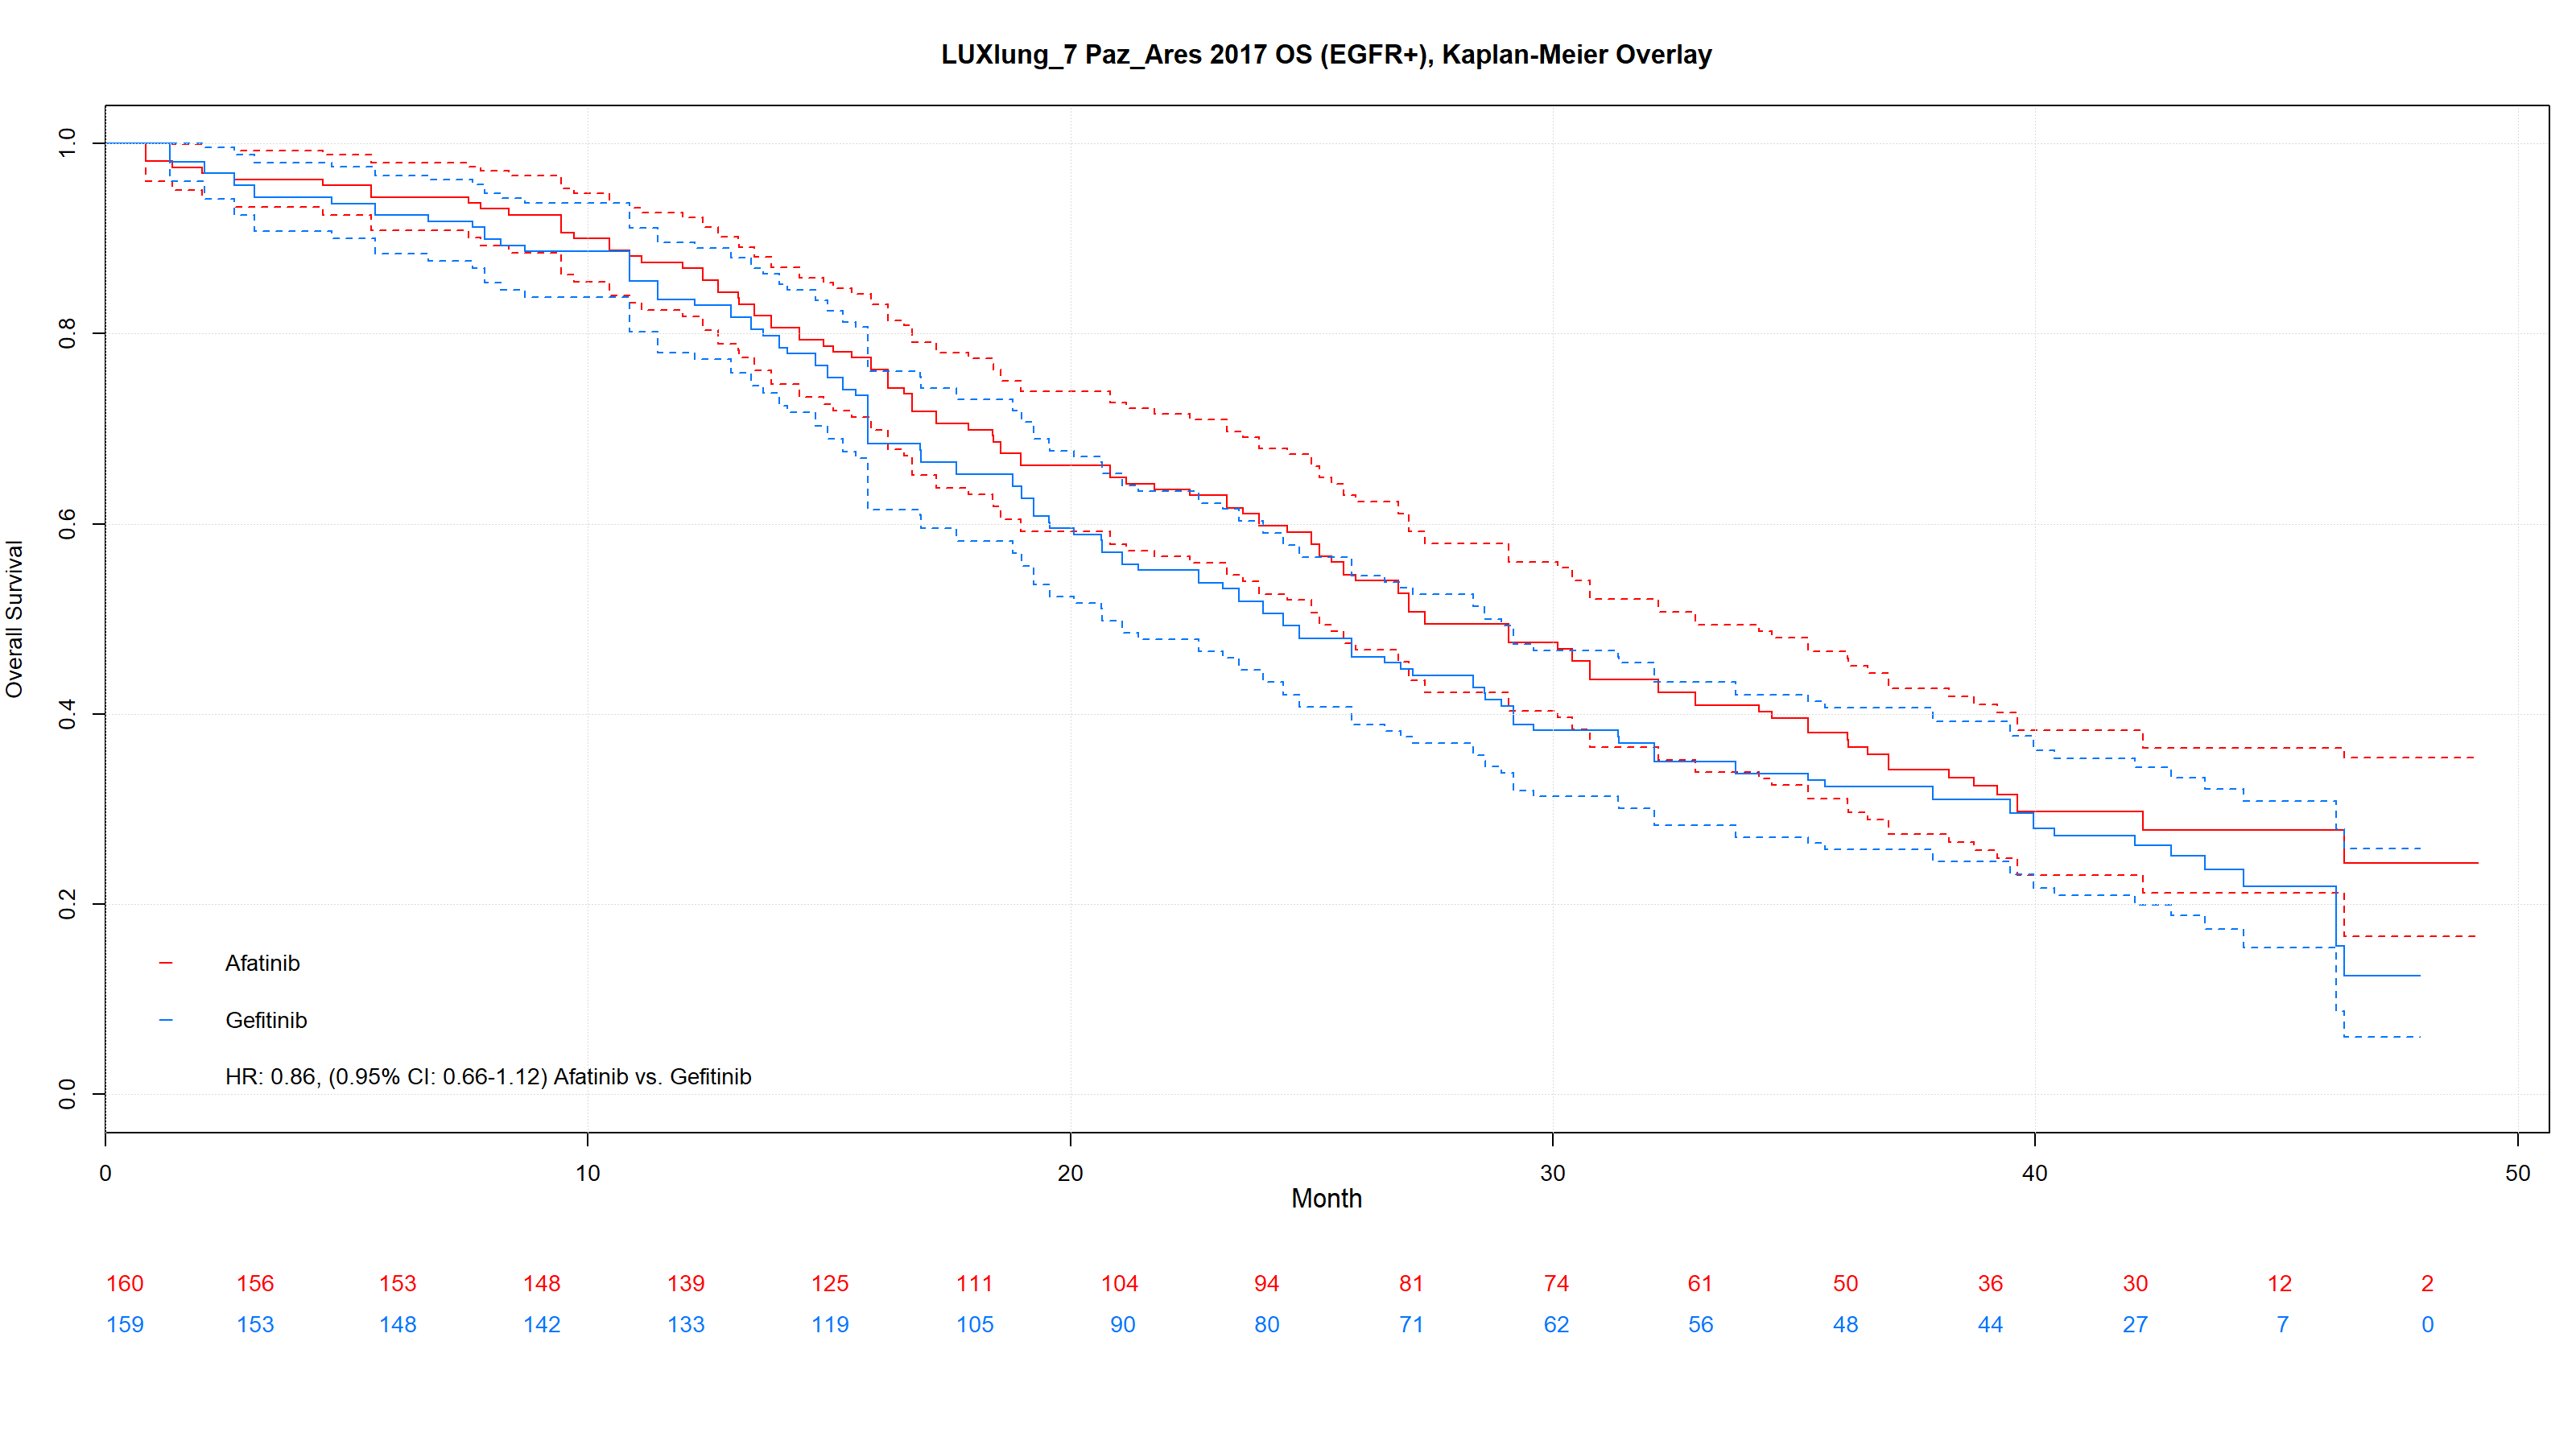
\includegraphics[max size={\textwidth}{\textheight}]{figs/km-plots/LUXlung_7 Paz_Ares 2017 OS (EGFR+) Kaplan Meier.png}
\end{subfigure}
\centering
\caption{LUX-LUNG 7, progression-free survival and overall survival}\label{fig:LUX-LUNG 7}
\end{figure}


\begin{figure}
\centering
\begin{subfigure}{\textwidth}
\centering
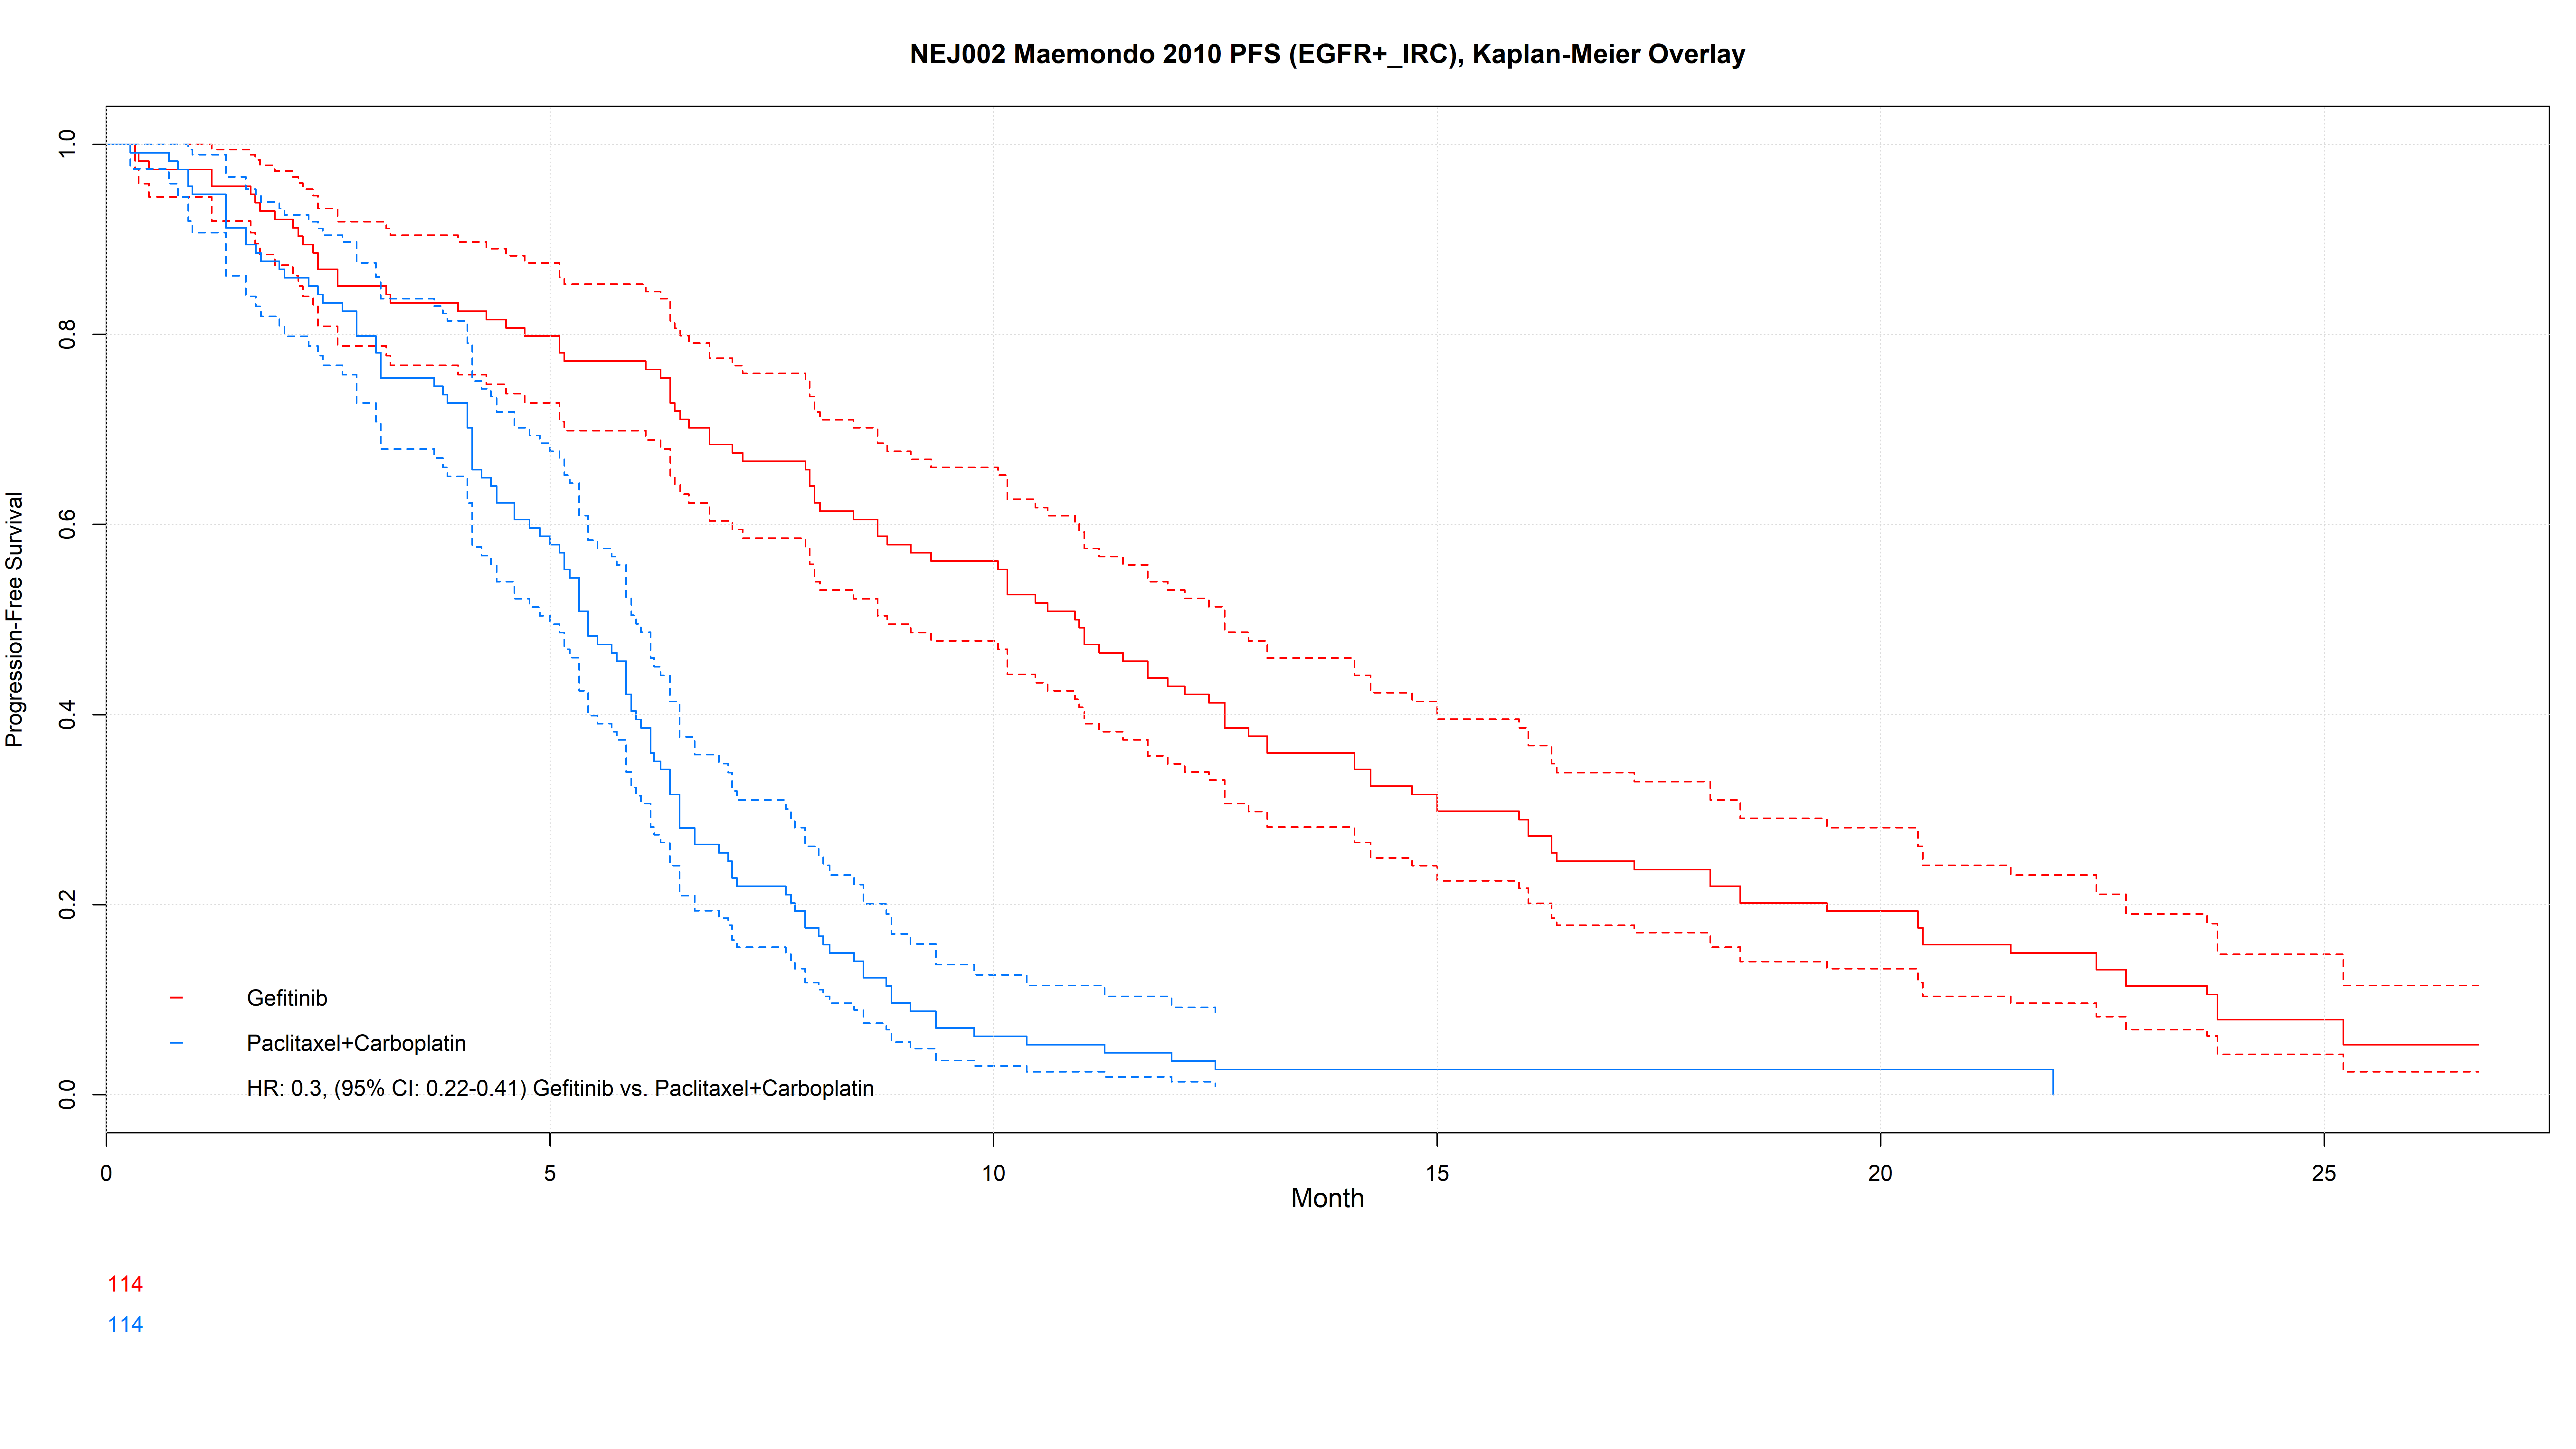
\includegraphics[max size={\textwidth}{\textheight}]{figs/km-plots/NEJ002 Maemondo 2010 PFS (EGFR+_IRC) Kaplan Meier.png}
\end{subfigure}
\begin{subfigure}{\textwidth}
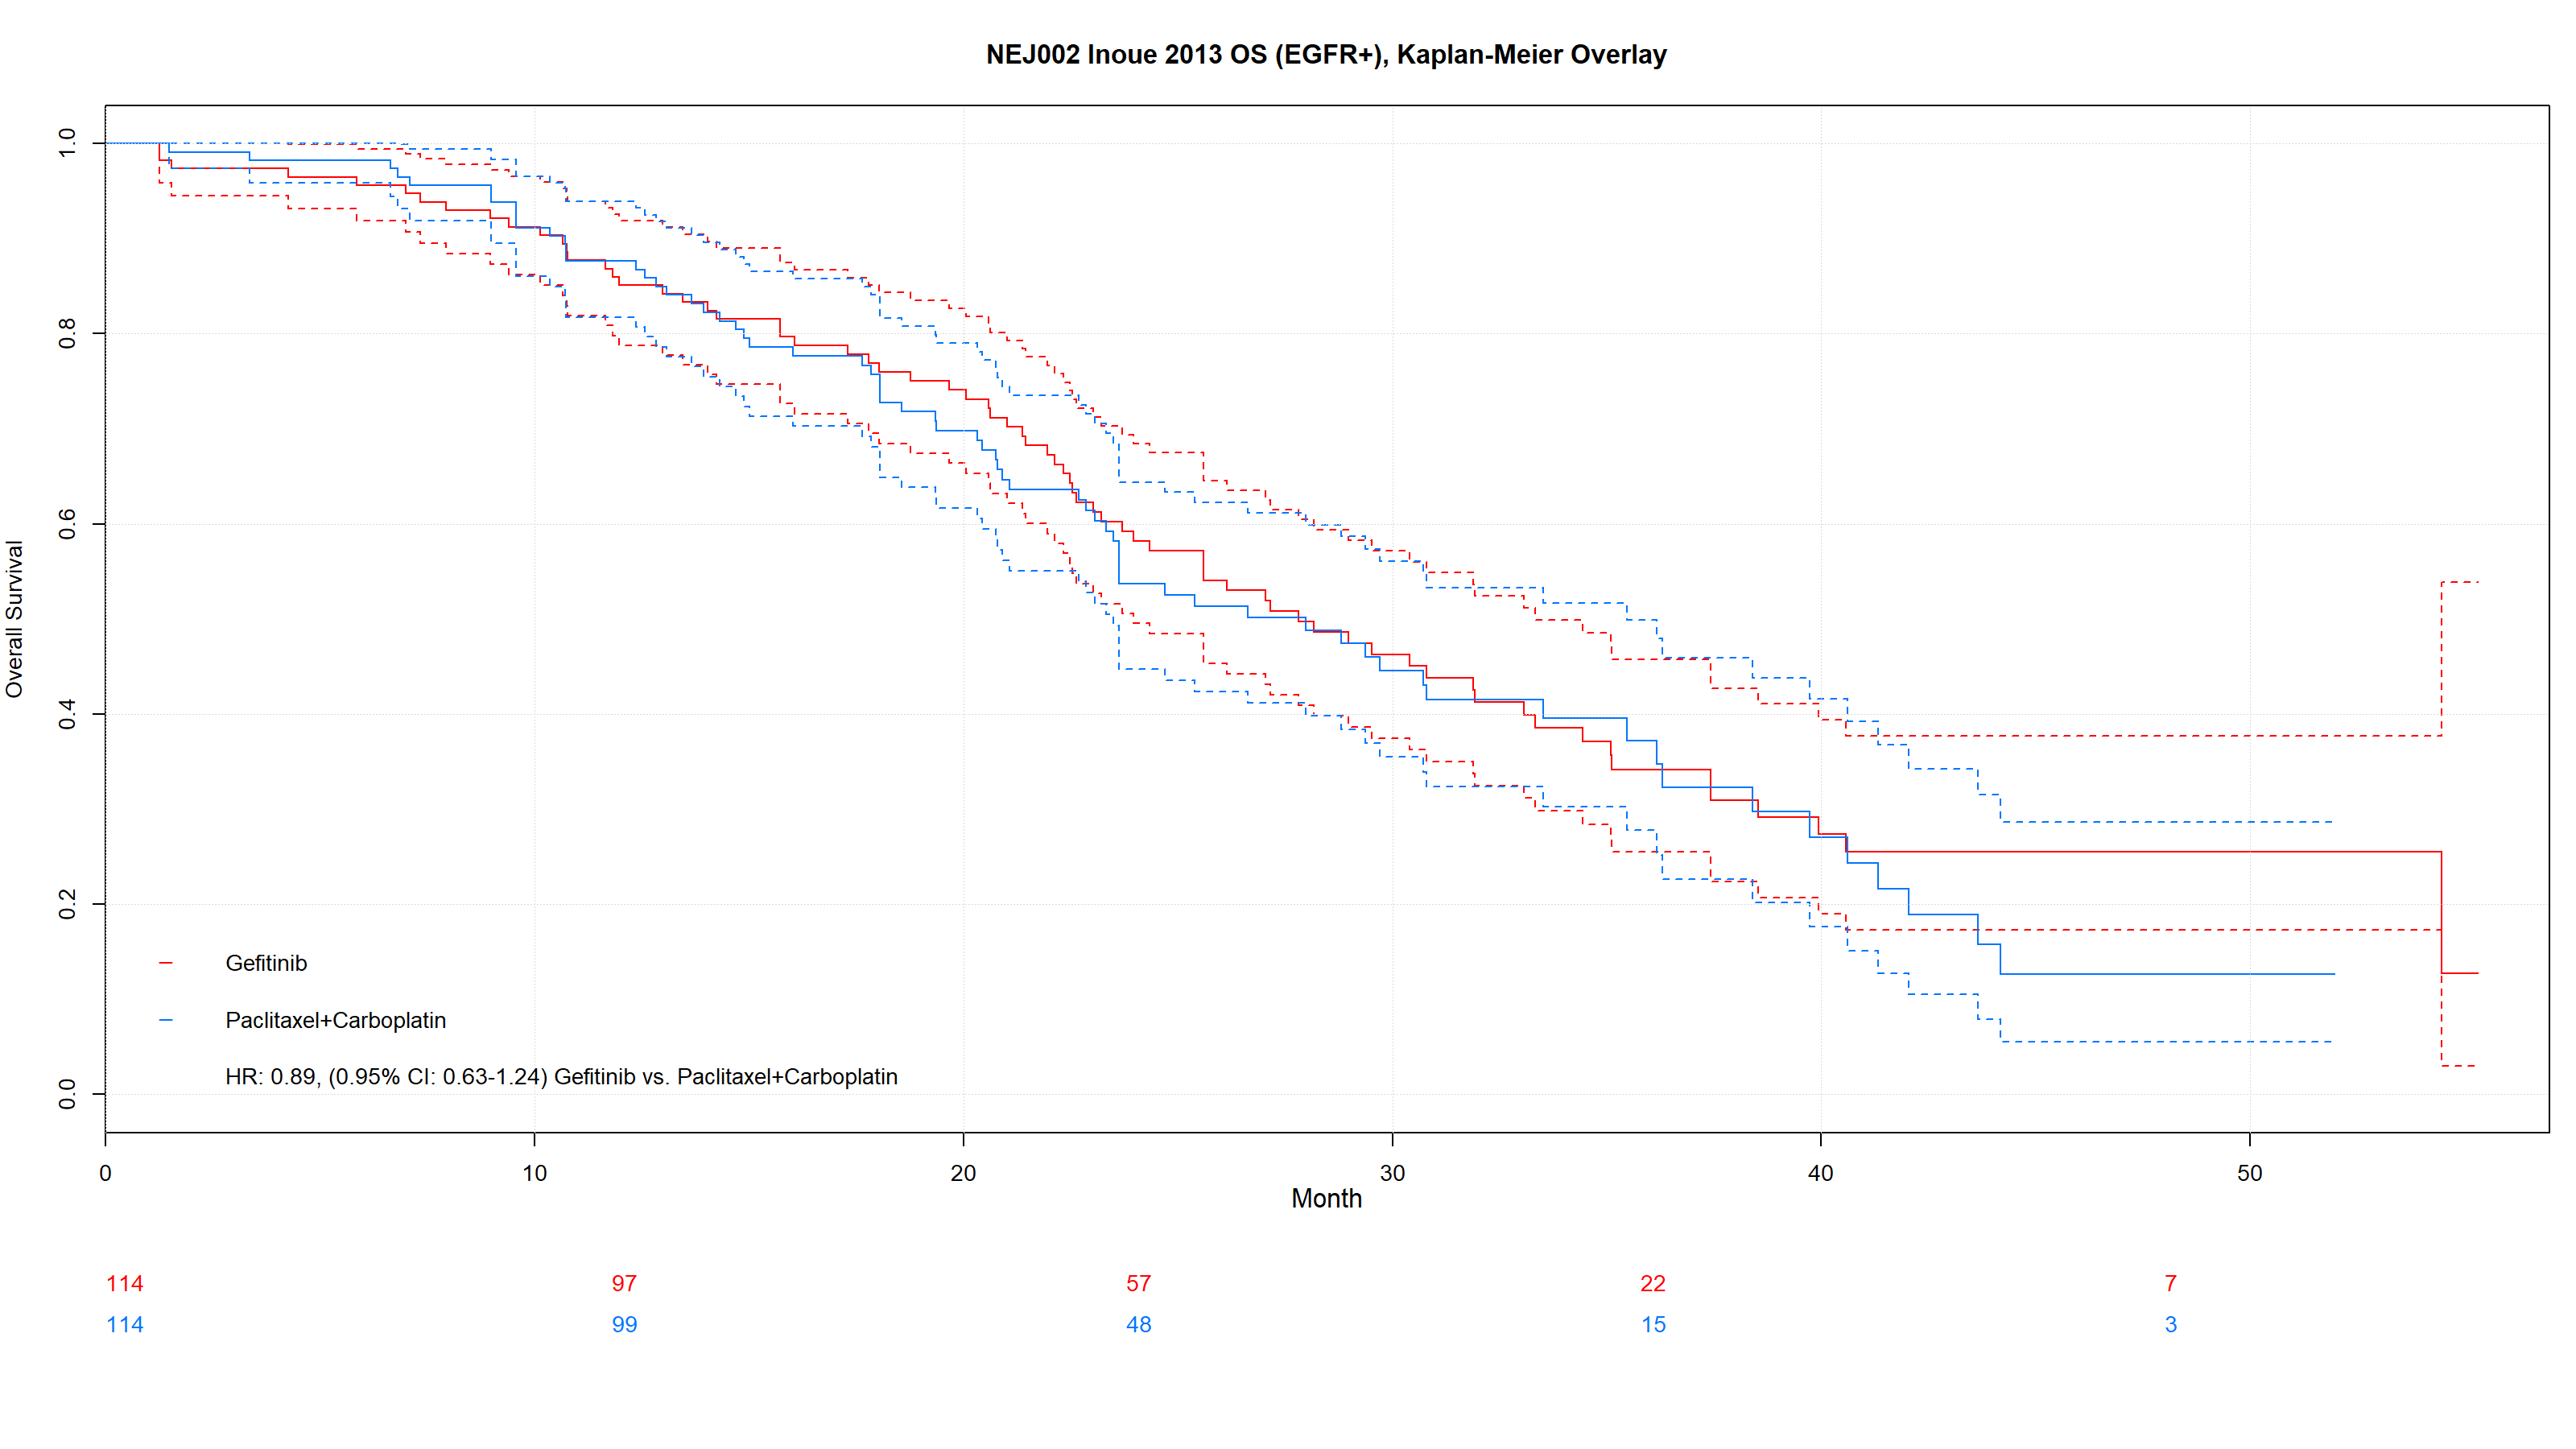
\includegraphics[max size={\textwidth}{\textheight}]{figs/km-plots/NEJ002 Inoue 2013 OS (EGFR+) Kaplan Meier.png}
\end{subfigure}
\centering
\caption{NEJ002, progression-free survival and overall survival}\label{fig:NEJ002}
\end{figure}


\begin{figure}
\centering
\begin{subfigure}{\textwidth}
\centering
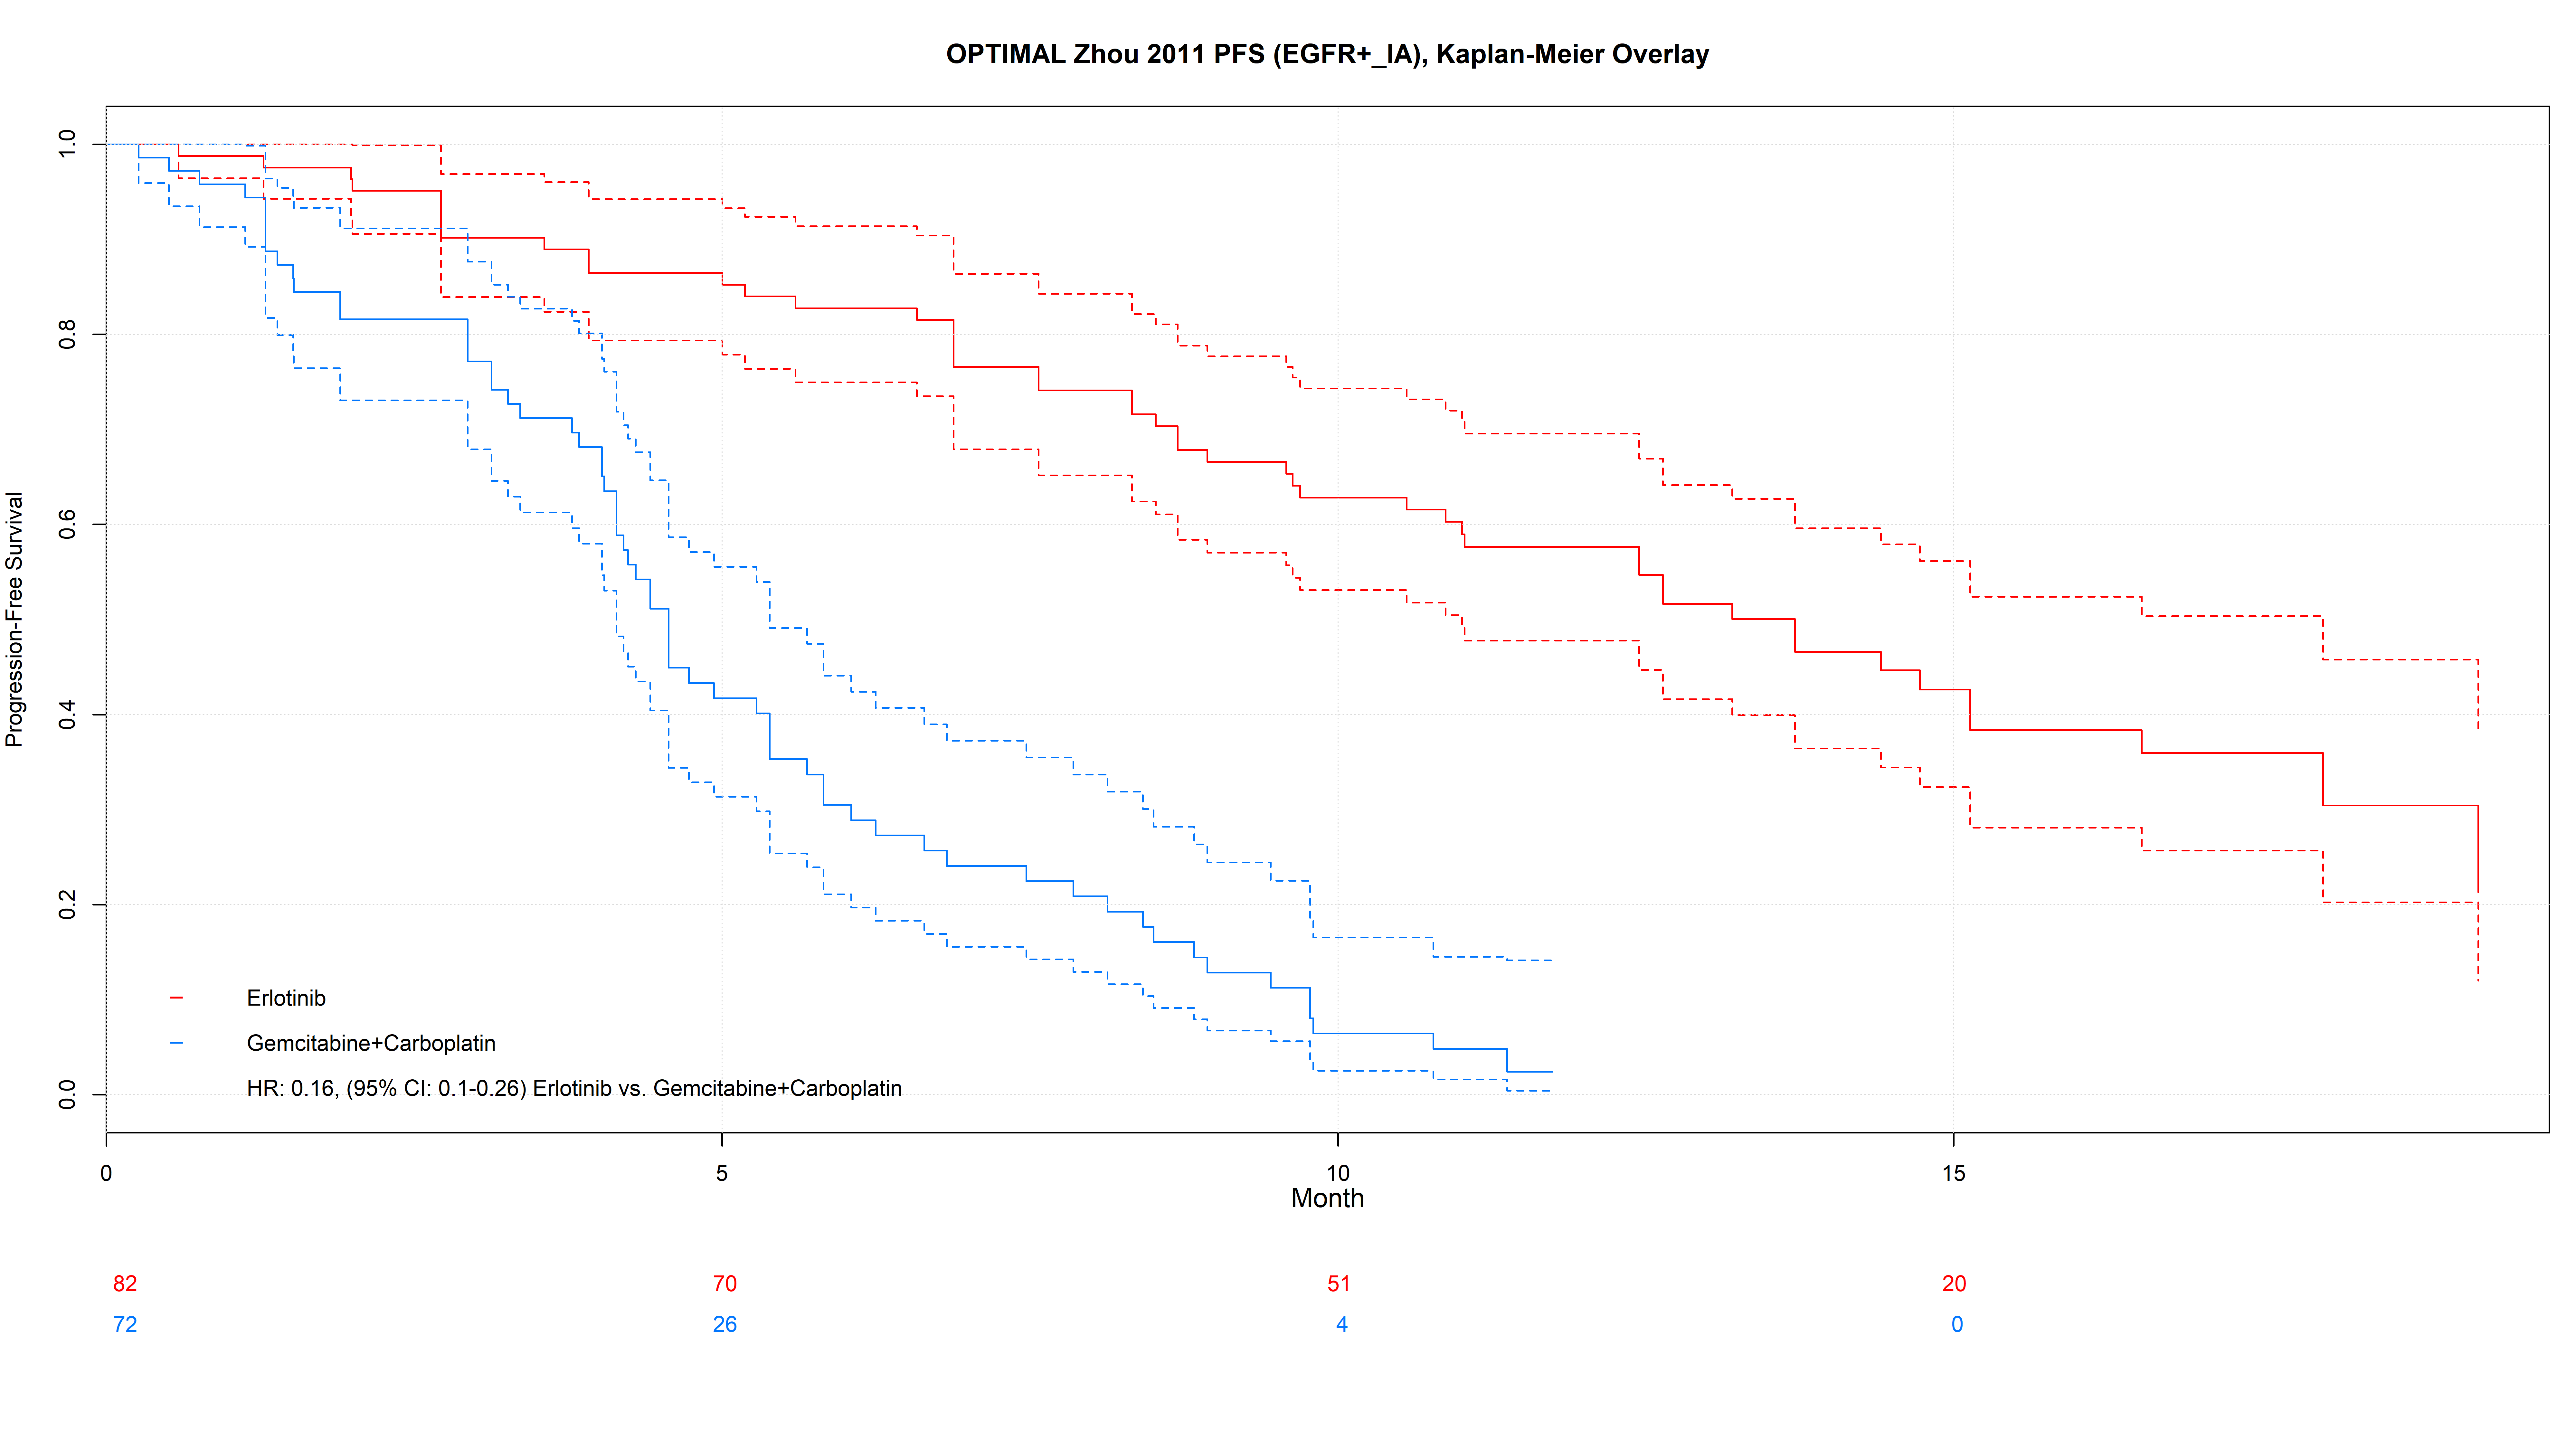
\includegraphics[max size={\textwidth}{\textheight}]{figs/km-plots/OPTIMAL Zhou 2011 PFS (EGFR+_IA) Kaplan Meier.png}
\end{subfigure}
\begin{subfigure}{\textwidth}
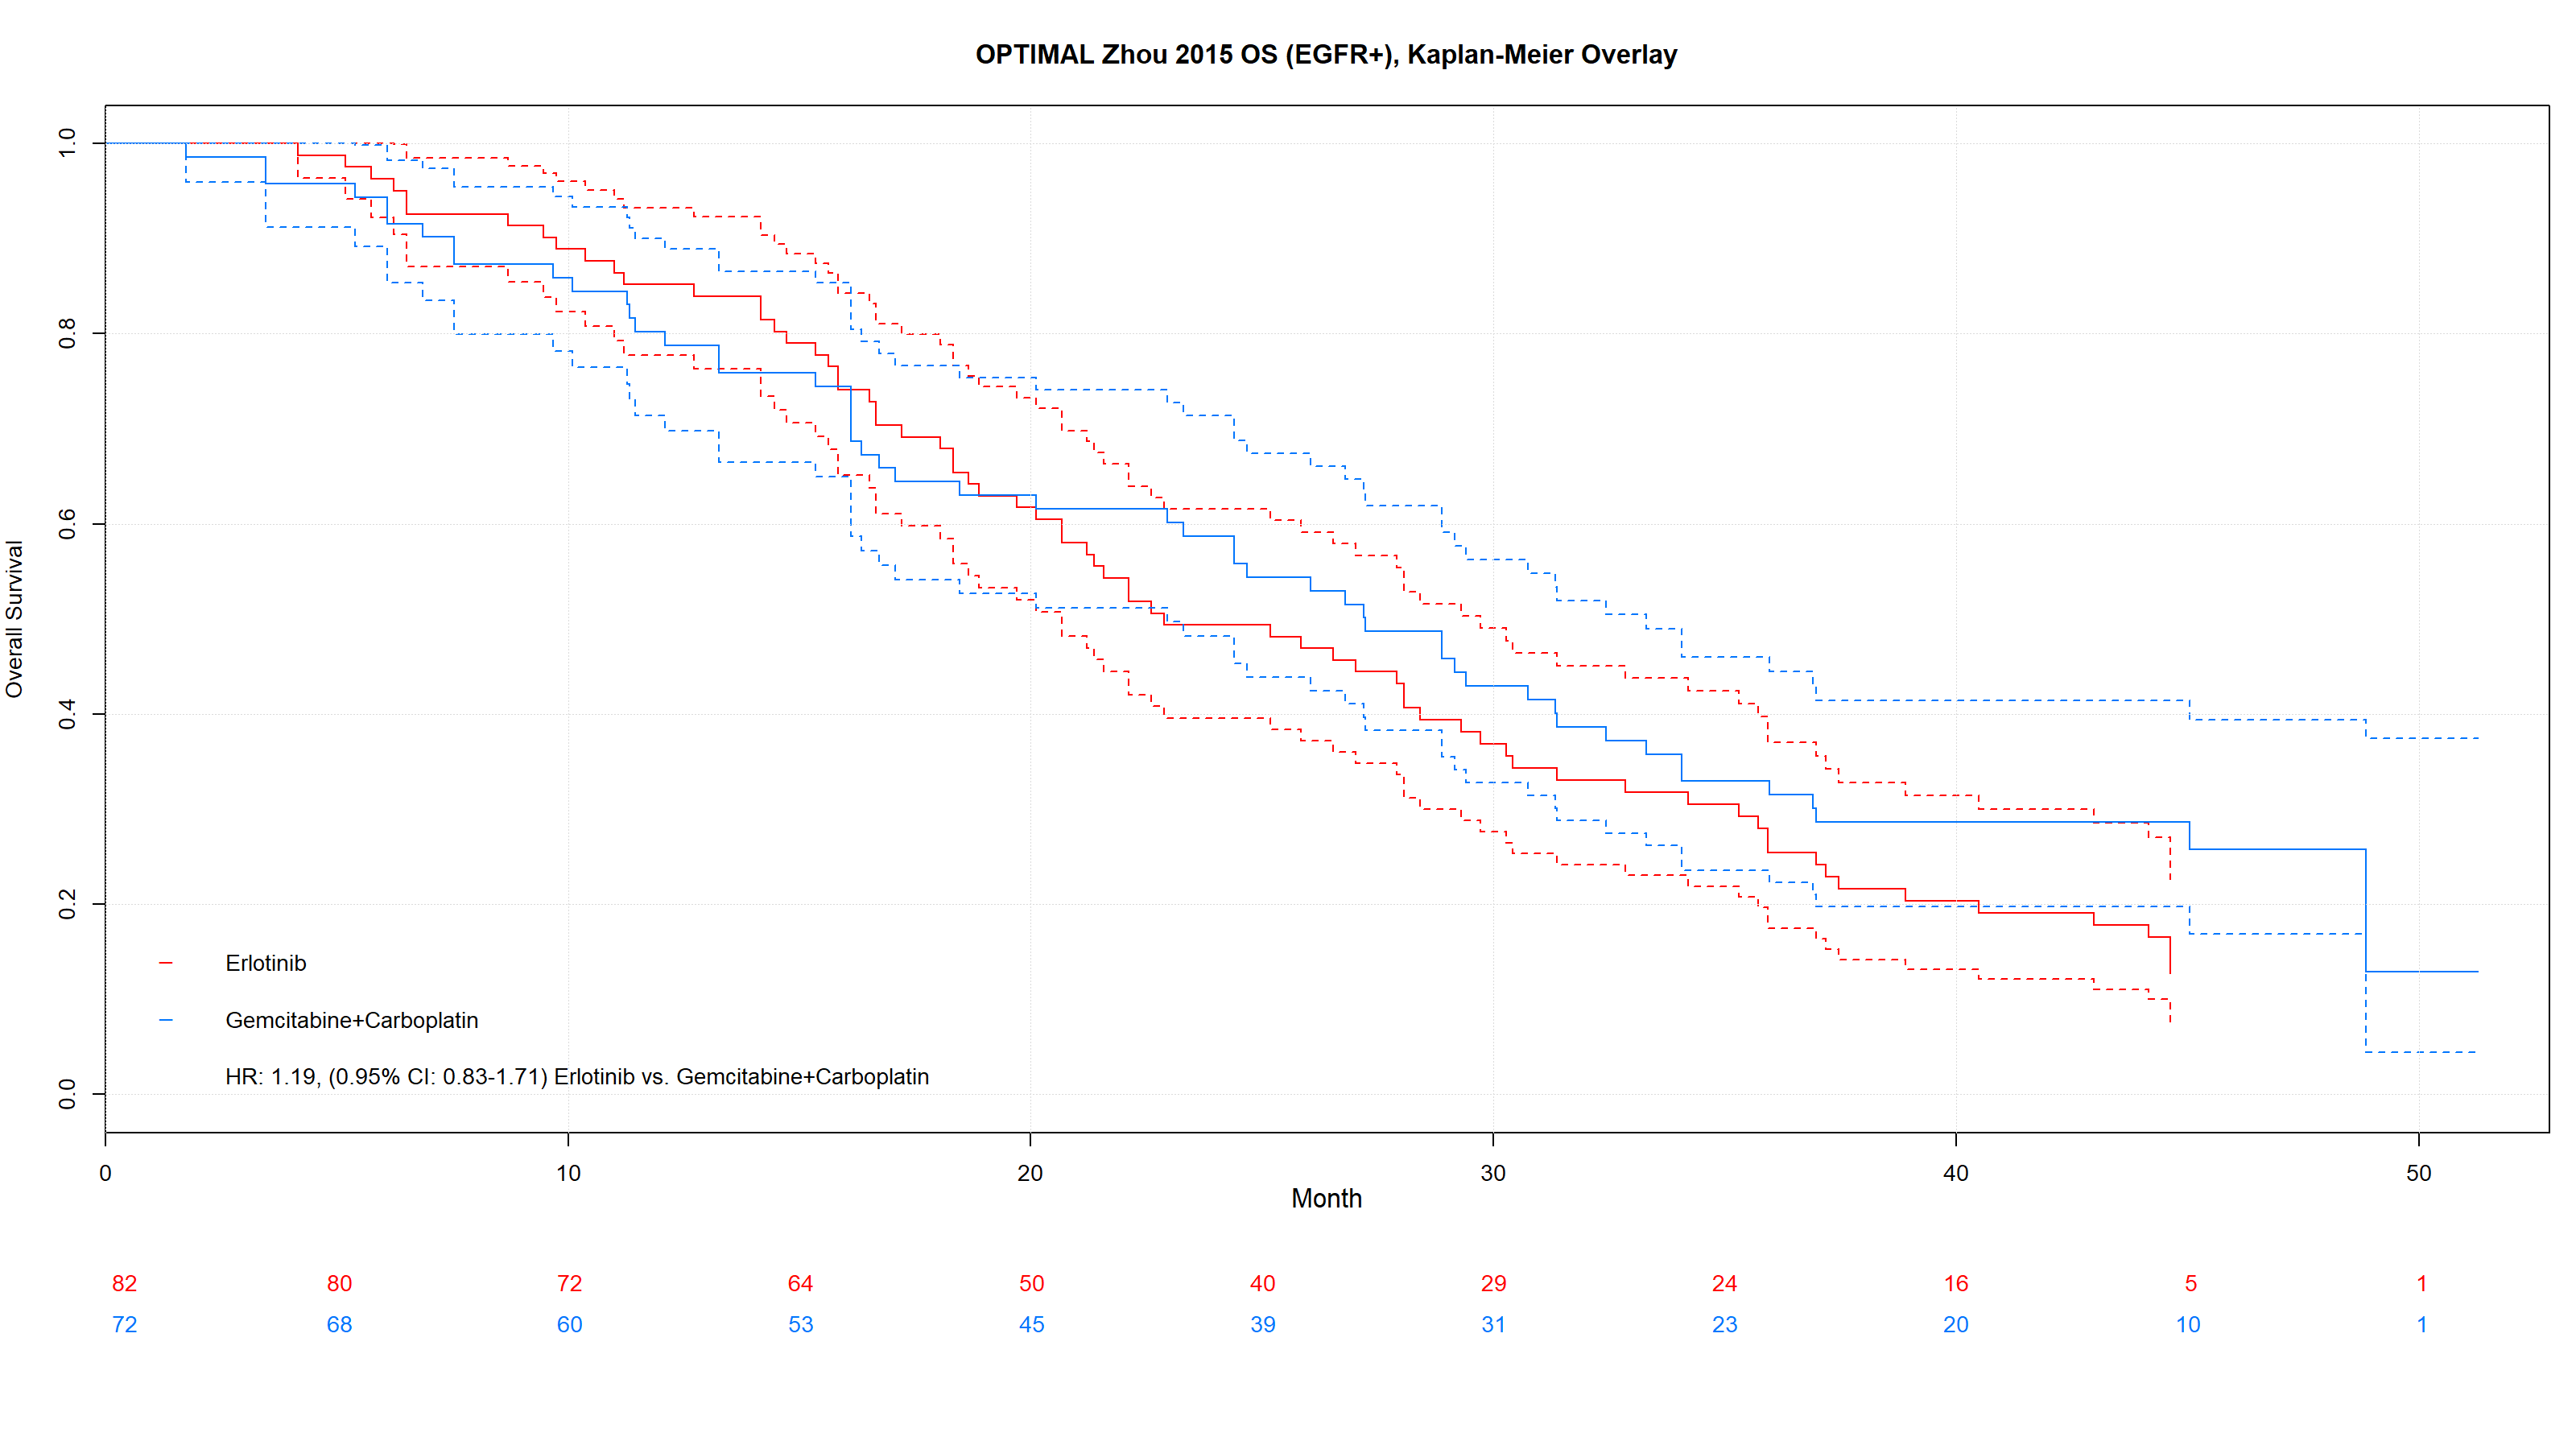
\includegraphics[max size={\textwidth}{\textheight}]{figs/km-plots/OPTIMAL Zhou 2015 OS (EGFR+) Kaplan Meier.png}
\end{subfigure}
\centering
\caption{OPTIMAL, progression-free survival and overall survival}\label{fig:OPTIMAL}
\end{figure}


\begin{figure}
\centering
\begin{subfigure}{\textwidth}
\centering
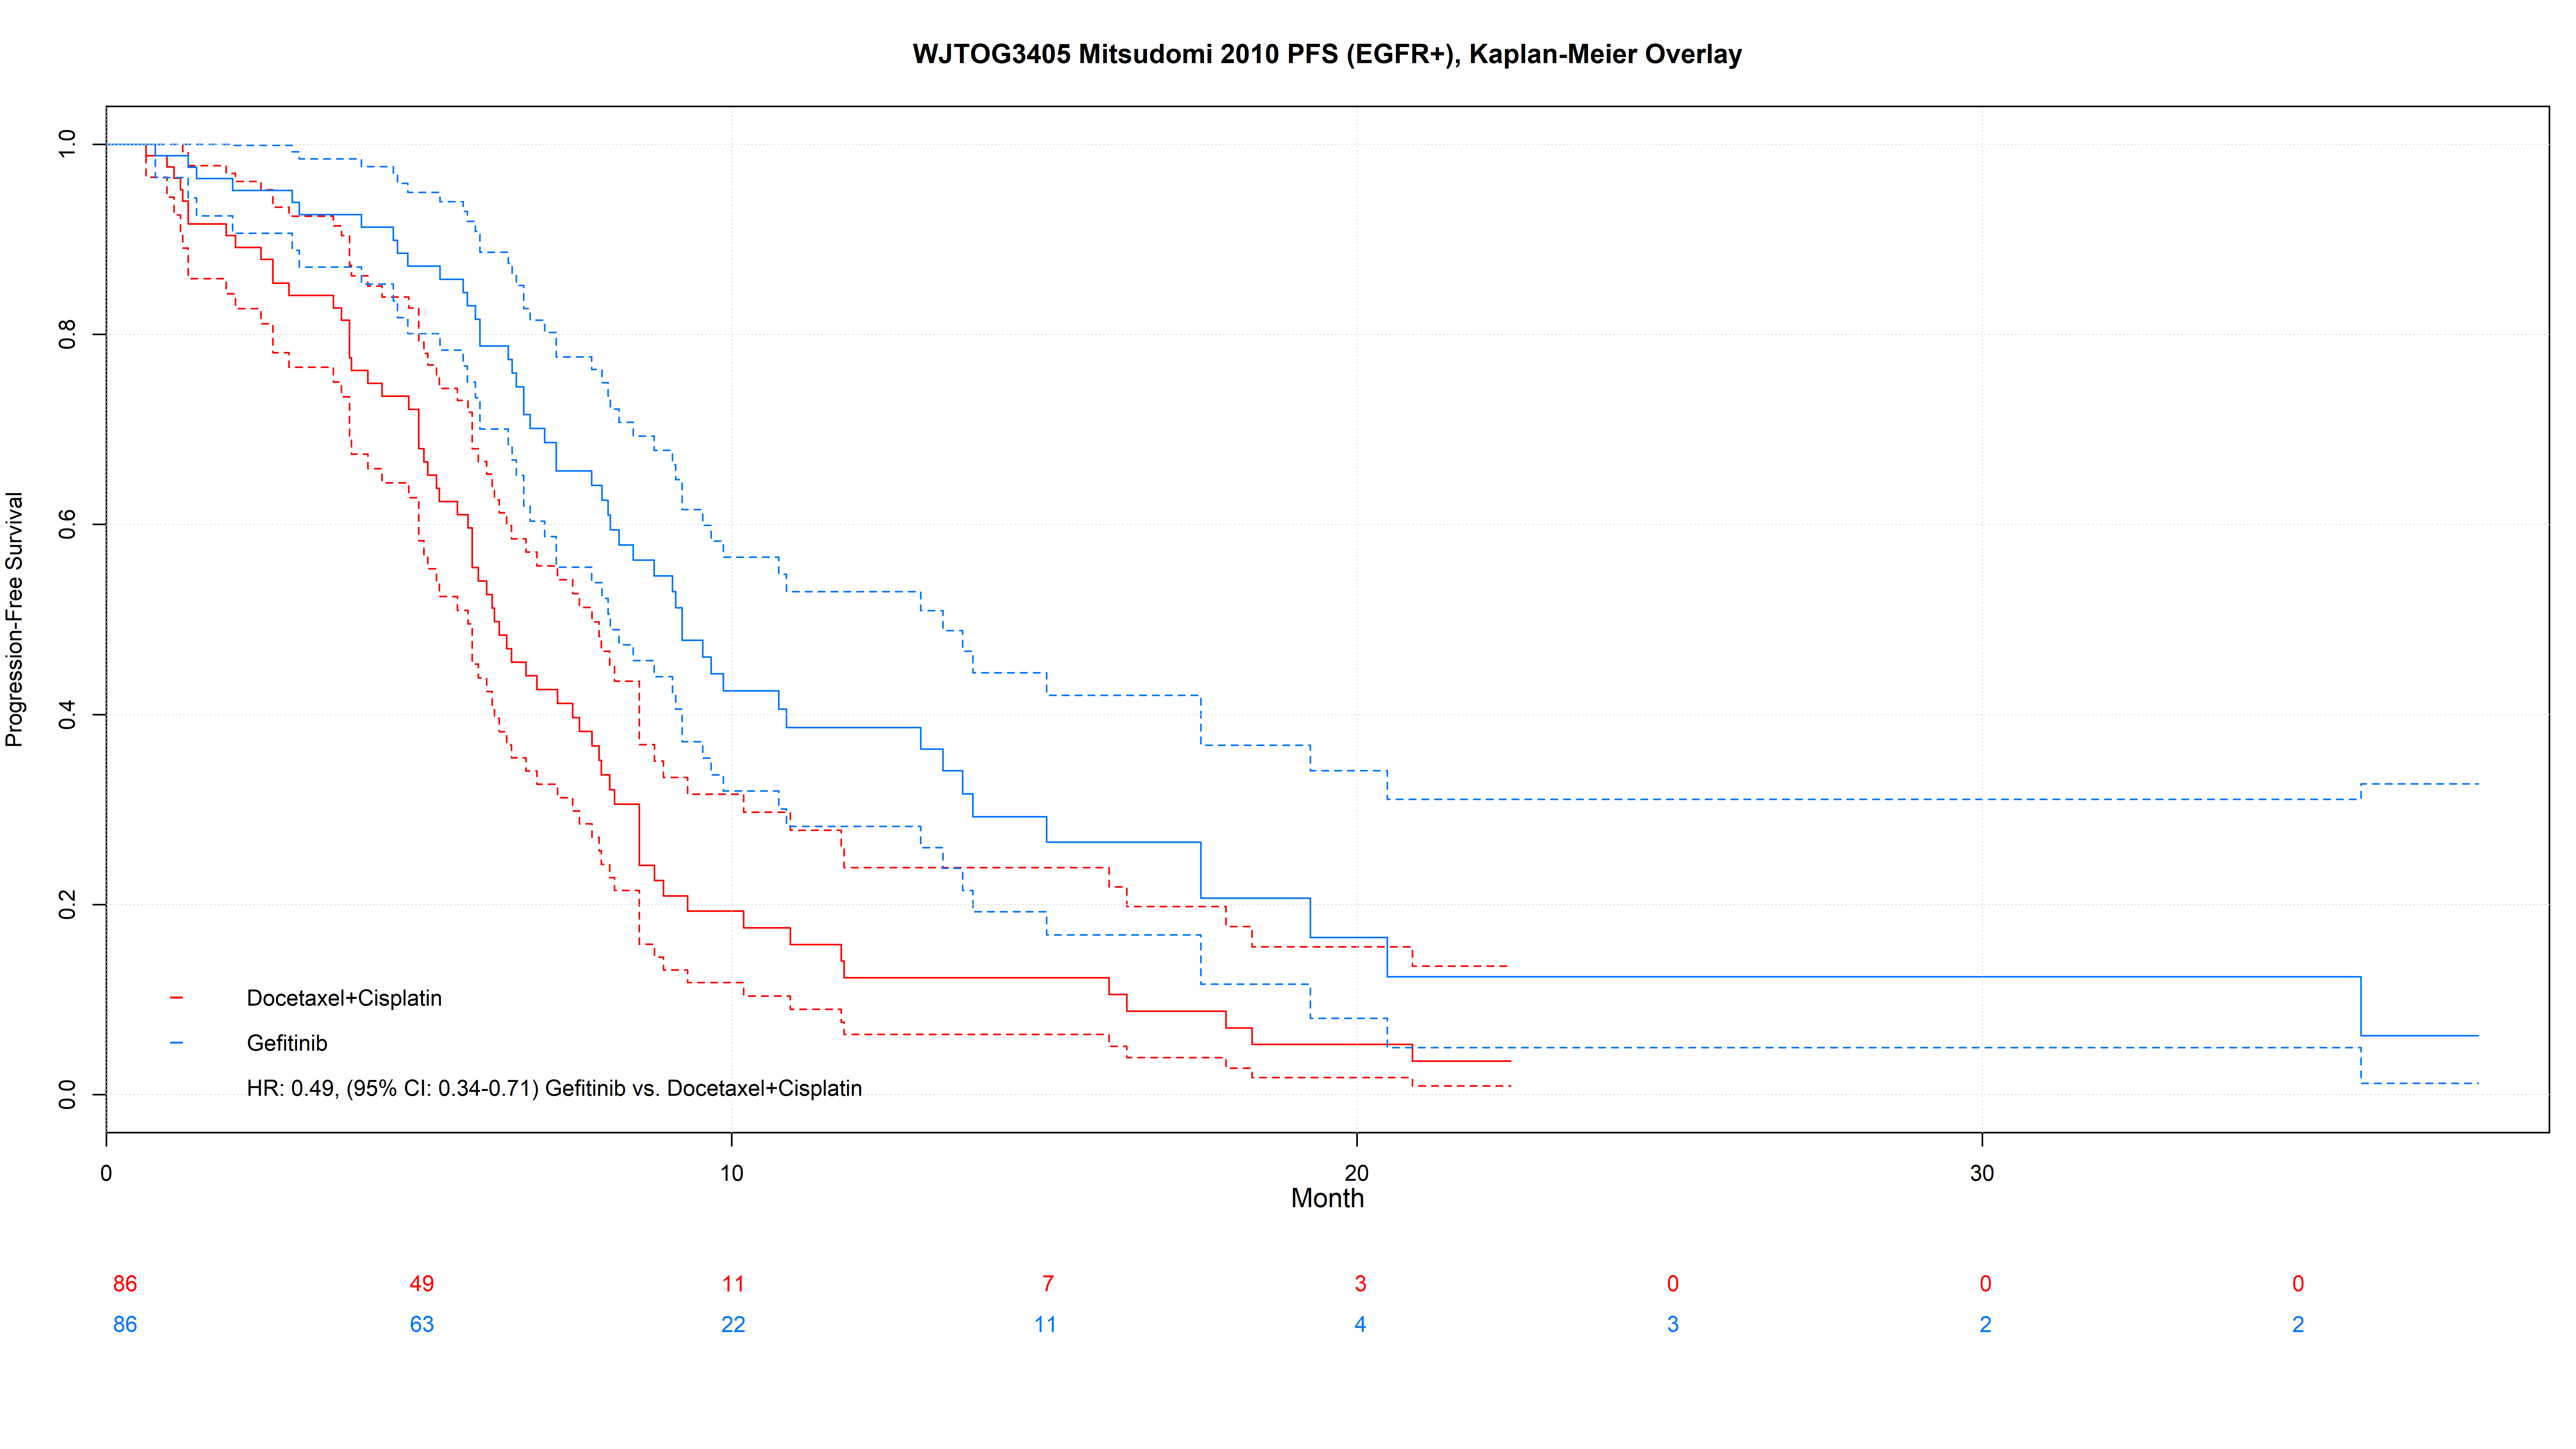
\includegraphics[max size={\textwidth}{\textheight}]{figs/km-plots/WJTOG3405 Mitsudomi 2010 PFS (EGFR+) Kaplan Meier.png}
\end{subfigure}
\begin{subfigure}{\textwidth}
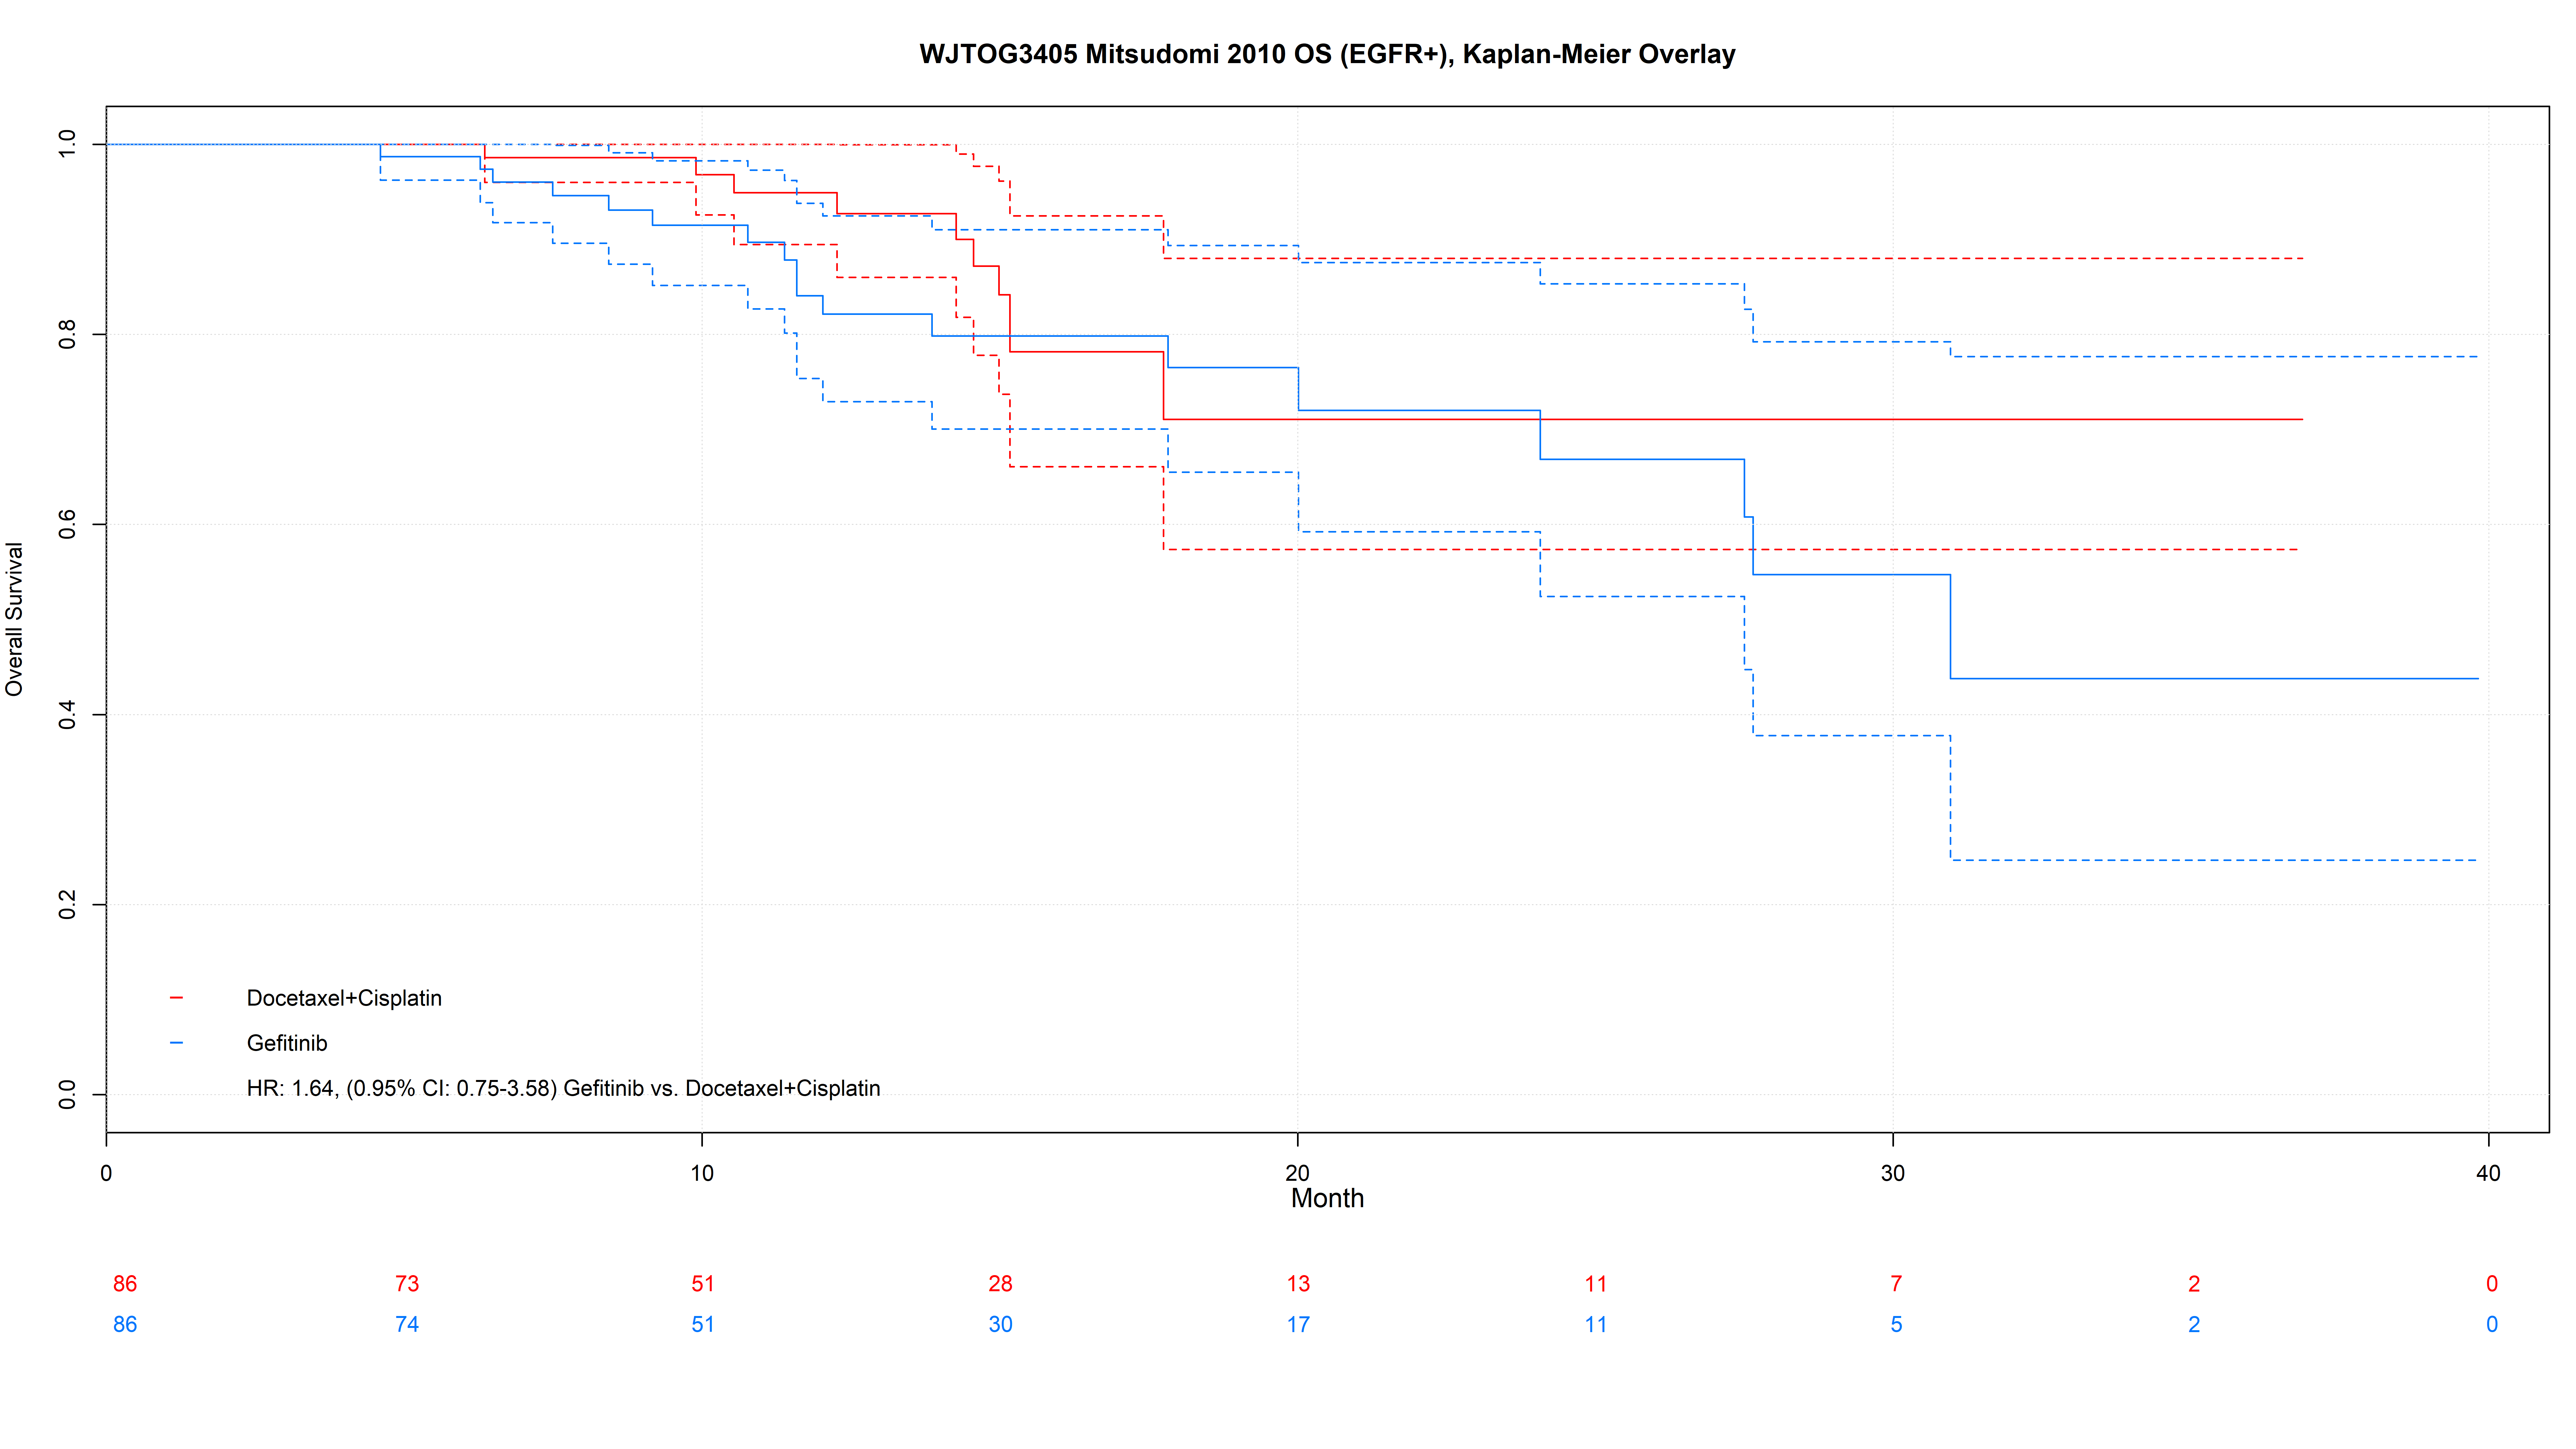
\includegraphics[max size={\textwidth}{\textheight}]{figs/km-plots/WJTOG3405 Mitsudomi 2010 OS (EGFR+) Kaplan Meier.png}
\end{subfigure}
\centering
\caption{WJTOG3405, progression-free survival and overall survival}\label{fig:WJTOG3405}
\end{figure}


\begin{figure}
\centering
\begin{subfigure}{\textwidth}
\centering
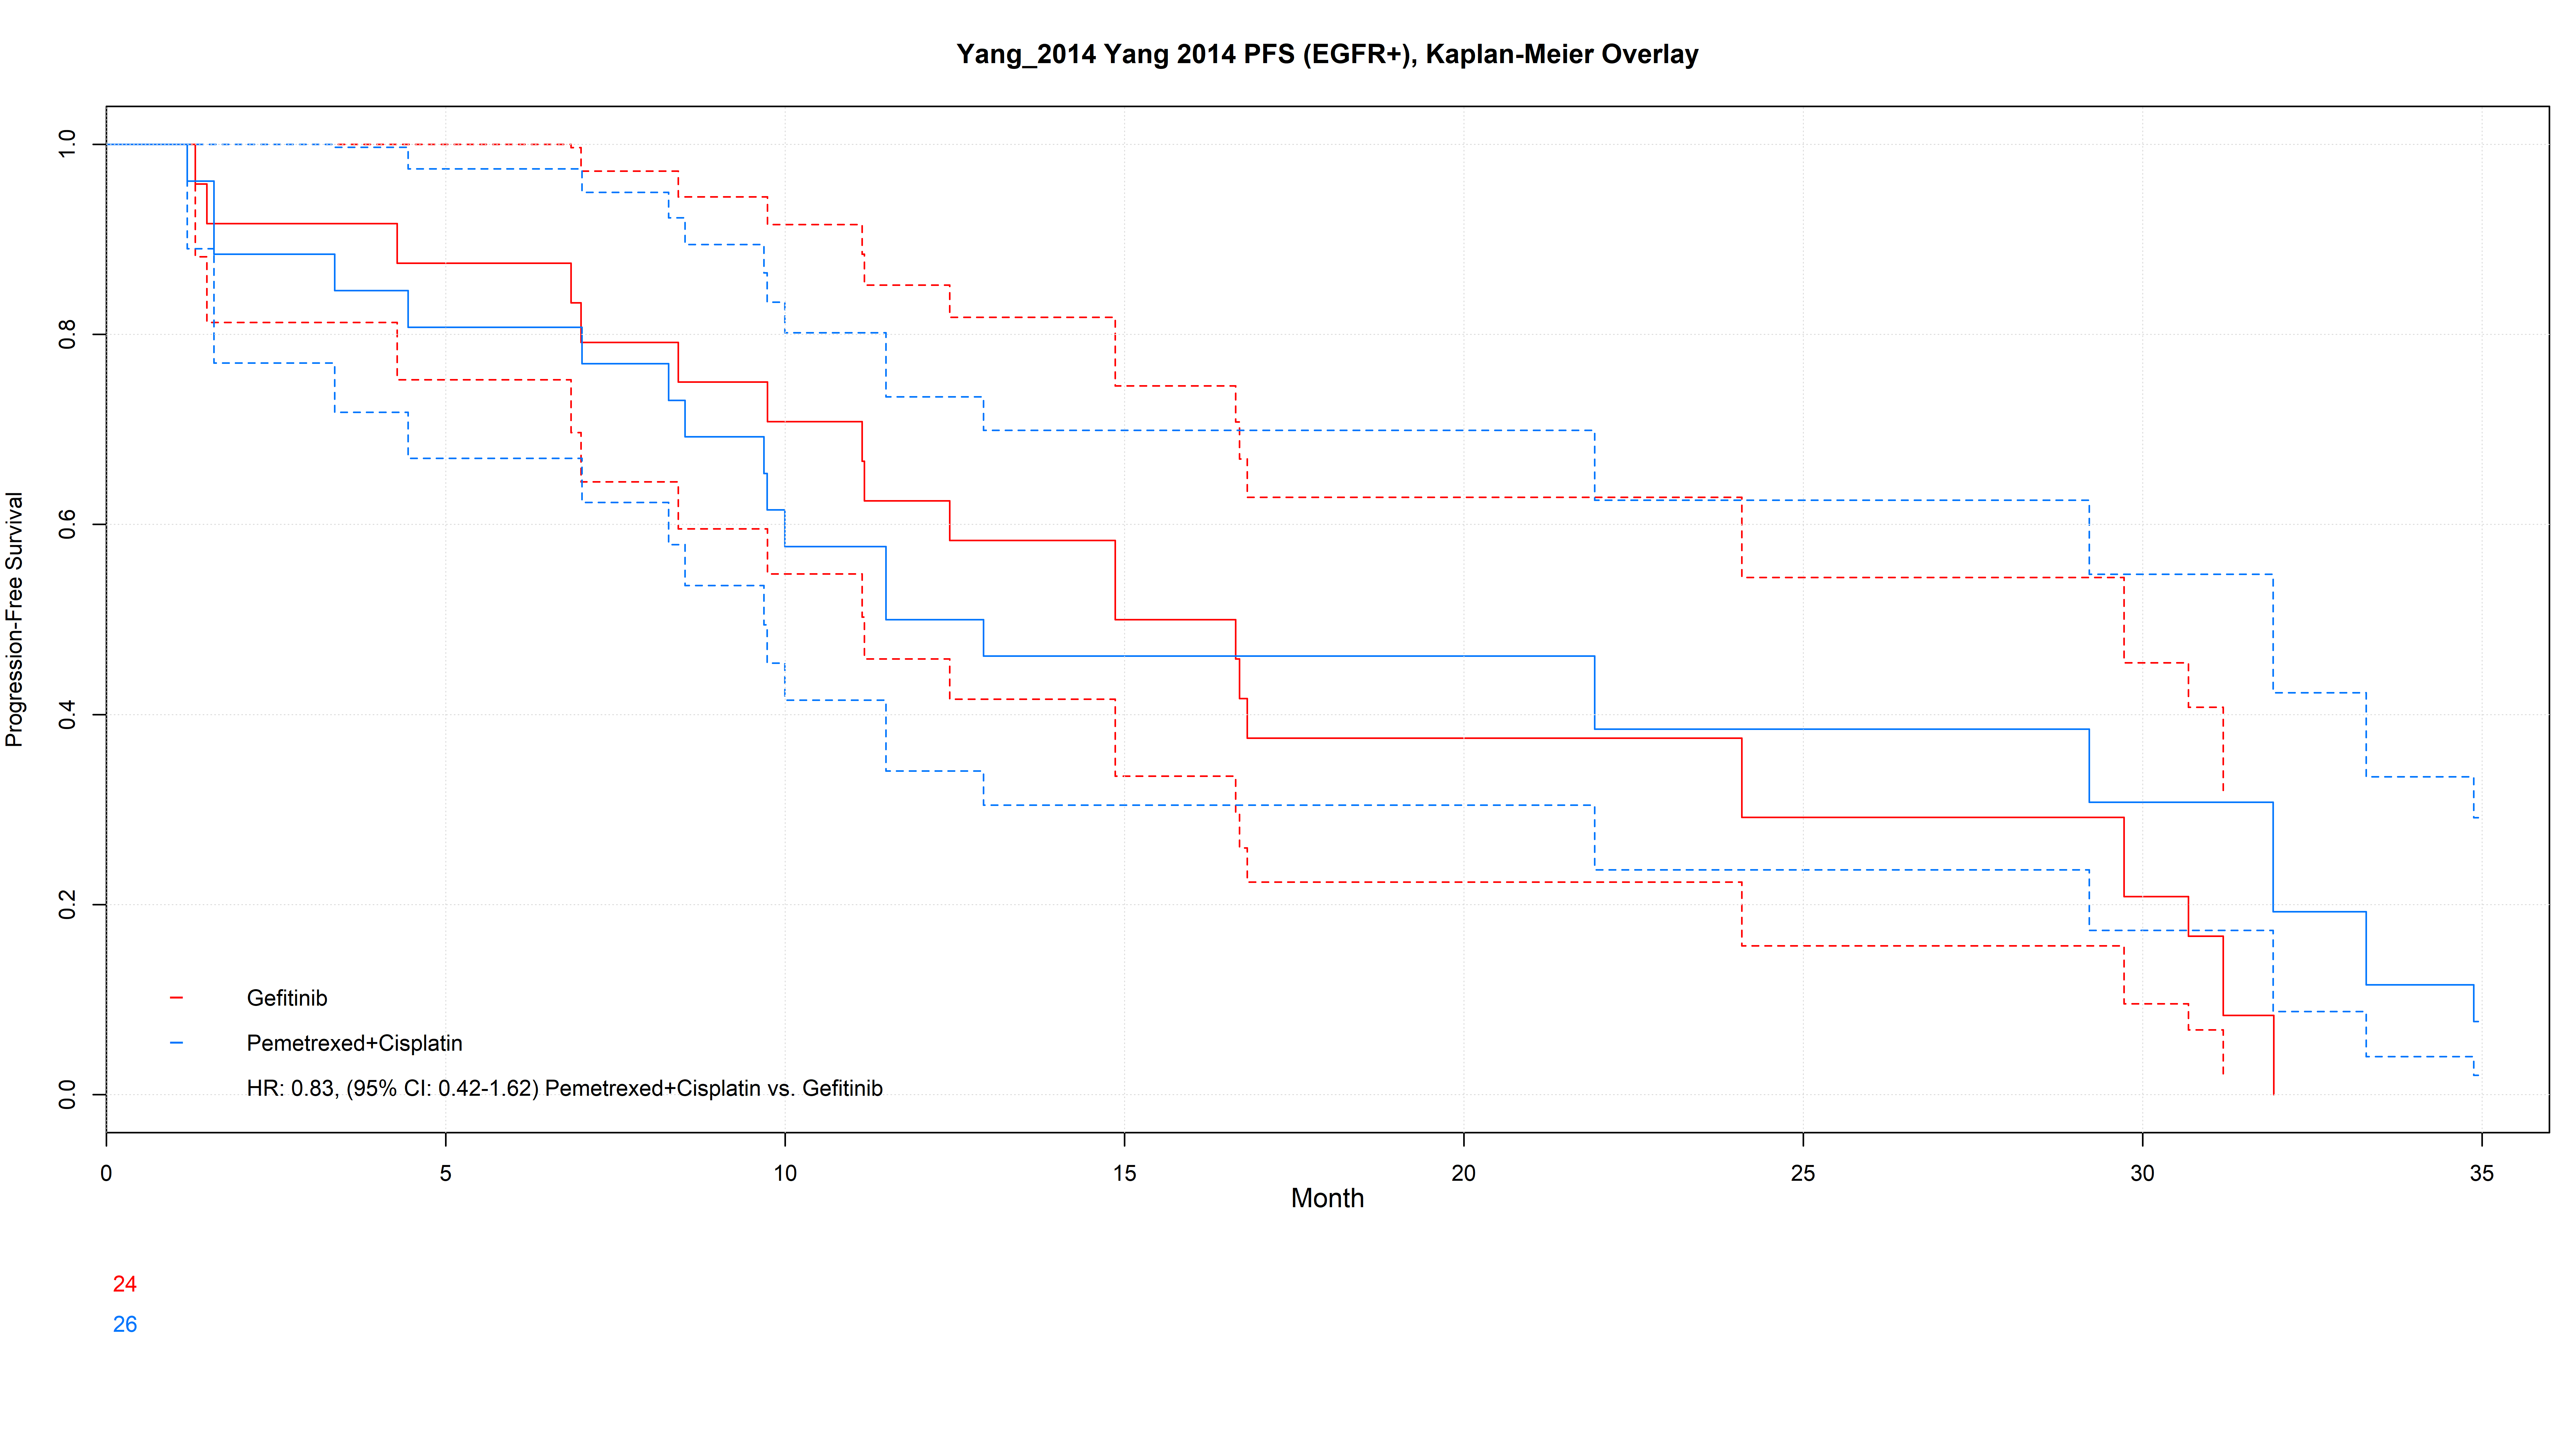
\includegraphics[max size={\textwidth}{\textheight}]{figs/km-plots/Yang_2014 Yang 2014 PFS (EGFR+) Kaplan Meier.png}
\end{subfigure}
\begin{subfigure}{\textwidth}
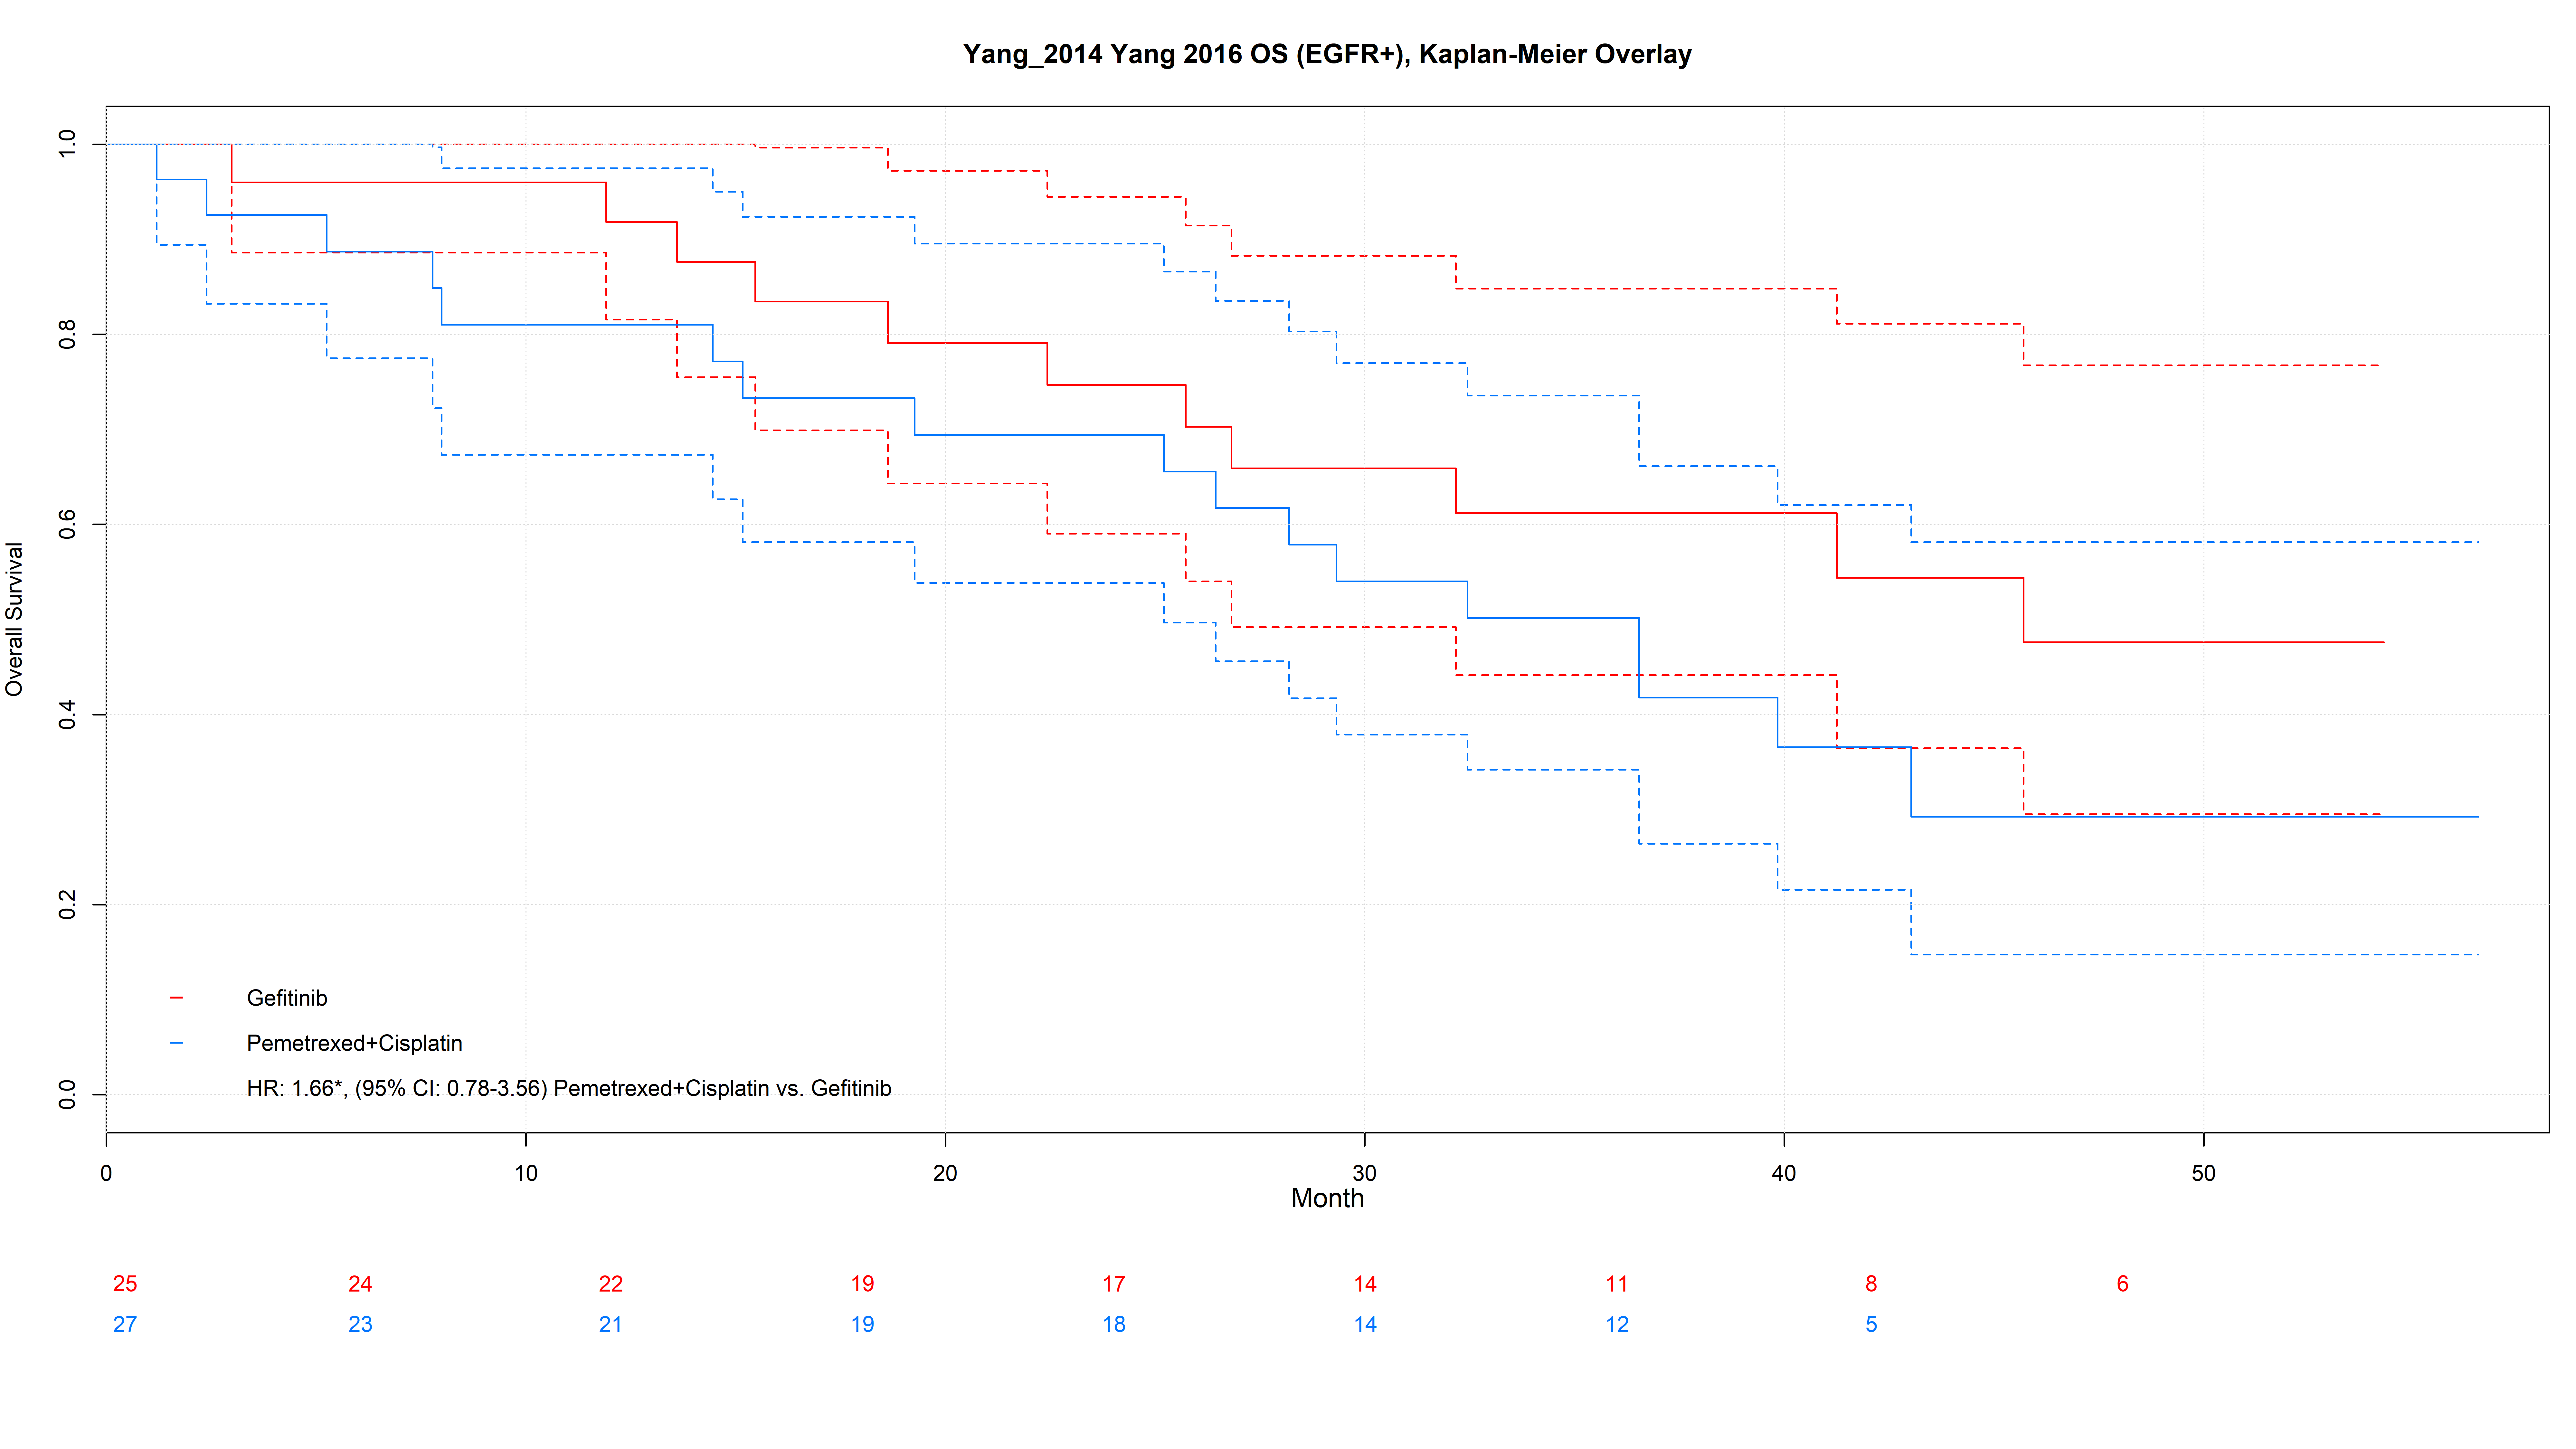
\includegraphics[max size={\textwidth}{\textheight}]{figs/km-plots/Yang_2014 Yang 2016 OS (EGFR+) Kaplan Meier.png}
\end{subfigure}
\centering
\caption{Yang 2014, progression-free survival and overall survival}\label{fig:Yang 2014}
\end{figure}
\fi

\section{Value of hope} \label{app:value-of-hope}
The value of hope measures the value patients place on tail-of-the-curve survival gains above and beyond what they place on increases in expected survival. It is computed for a given treatment strategy $k$ relative to a reference treatment $1$ by first estimating the certainty equivalent, or the life-years a patient would need to obtain to be indifference between treatment $k$ and the reference treatment (treatment $1$). To facilitate CEA, we work with QALYs rather than life-years. We assume a constant relative risk aversion utility function for QALYs $x$ of the form,

\begin{equation}\label{eqn:value-of-hope}
u(x) = x^\eta,
\end{equation}

where $\eta$ is a measure of risks aversion with $\eta > 1$ implying that a patient is risk loving and $\eta < 1$ that a patient is risk averse. Using survey data from patients, \citet{shafrin2017patient} estimate $\eta = 1.39$ for NSCLC patients. The certainty equivalent, $\alpha_{k1}$, for treatment $k$ relative to the reference treatment is computed by solving,

\begin{equation}
\int u(x + \alpha_{k1}) f_k(x) dx = V_1,
\end{equation}    

where $f_k(x)$ is the distribution of QALYs for treatment $k$ and $V_1 = \int u(x)f_1(x) dx$ is expected utility for the reference treatment. In the model, $f_k(x)$ and $f_1(x)$ are estimated using the distribution of QALYs from the individual-level simulation. We solve for $\alpha_{k1}$ using the \R{} root finding algorithm $\lstinline[columns=fixed]{uniroot}$. 

The value of hope, $\theta$, is the difference between the certainty equivalent and differences in expected survival,

\begin{equation}
\theta = \alpha_{k1} - \left[E_k(x) - E_1(x) \right],
\end{equation}     

where $E_k(x)$ and $E_1(x)$ are mean QALYs for treatment $k$ and the reference arm, respectively. 

Note that since the algorithm is computationally intensive, we do not currently use the PSA to compute a distribution for $\theta$. Instead, we estimate a point estimate using the distribution of QALYs across all PSA iterations. Future work could speed up the algorithm so that it is fast enough for PSA by rewriting it in a compiled language such as \CPP{}.  

\end{appendices}
\pdfbookmark[1]{References}{References}
\bibliography{references}


\end{document}